%-----------------------------------------------------------------------
%
% filename = nube.tex
%
% First version: February 2012
% Last revision: April 2012
%
%-----------------------------------------------------------------------

\documentclass[twocolumn,aps,showpacs,showkeys,prd,superscriptaddress,byrevtex, amsmath]{revtex4-1}


%%%%%%%%%%%%%%%%%%%%%%%%%
%%%   LOAD PACKAGES   %%%
%%%%%%%%%%%%%%%%%%%%%%%%%
 
\usepackage{amssymb}
\usepackage{amsmath}
\usepackage{verbatim}
\usepackage{mathrsfs}
\usepackage{amsfonts}
\usepackage{latexsym}
\usepackage{epsfig}
\usepackage{color}
\usepackage{graphicx,subfigure}
\usepackage{units}
\usepackage{slashbox}
\usepackage{aas_macros}



%%%%%%%%%%%%%%%%%%%%%%%%%
%%%   BEGIN DOCUMENT  %%%
%%%%%%%%%%%%%%%%%%%%%%%%%

\begin{document}


%%%%%%%%%%%%%%%%%%
%%%   MACROS   %%%
%%%%%%%%%%%%%%%%%%

\renewcommand{\t}{\times}
\newcommand{\sg}[1]{\textcolor{blue}{SG: #1}}
\newcommand{\tf}[1]{\textcolor{red}{TF: #1}}

\long\def\symbolfootnote[#1]#2{\begingroup%
\def\thefootnote{\fnsymbol{footnote}}\footnote[#1]{#2}\endgroup}


%%%%%%%%%%%%%%%%%
%%%   TITLE   %%%
%%%%%%%%%%%%%%%%%

\title{Magnetized accretion disks around Kerr black holes with scalar hair - I. Constant angular momentum disks} 

\author{Sergio Gimeno-Soler}
\affiliation{Departamento de
  Astronom\'{\i}a y Astrof\'{\i}sica, Universitat de Val\`encia,
  C/ Dr. Moliner 50, 46100, Burjassot (Val\`encia), Spain}

\author{Jos\'e A. Font}
\affiliation{Departamento de
  Astronom\'{\i}a y Astrof\'{\i}sica, Universitat de Val\`encia,
  C/ Dr. Moliner 50, 46100, Burjassot (Val\`encia), Spain}
\affiliation{Observatori Astron\`omic, Universitat de Val\`encia, C/ Catedr\'atico 
  Jos\'e Beltr\'an 2, 46980, Paterna (Val\`encia), Spain}

\author{Carlos Herdeiro}
\affiliation{Departamento de F\'{\i}sica da Universidade de Aveiro and CIDMA, Campus de Santiago, 
3810-183 Aveiro, Portugal}

\author{Eugen Radu}
\affiliation{Departamento de F\'{\i}sica da Universidade de Aveiro and CIDMA, Campus de Santiago, 
3810-183 Aveiro, Portugal}


%%%%%%%%%%%%%%%%
%%%   DATE   %%%
%%%%%%%%%%%%%%%%

\date{\today}


%%%%%%%%%%%%%%%%%%%%
%%%   ABSTRACT   %%%
%%%%%%%%%%%%%%%%%%%%

\begin{abstract} 
Testing the true nature of black holes -- the no-hair hypothesis -- will become increasingly more precise in the next few years as new observational data is collected in both the gravitational wave channel and the electromagnetic channel. In this work we consider numerically generated spacetimes of Kerr black holes with synchronised scalar hair and build stationary models of magnetized constant angular momentum thick disks around them. We study the dependence of the morphology and properties of the accretion tori on the type of black hole considered, from purely Kerr black holes with varying degrees of  spin parameter to Kerr black holes with scalar hair with different ADM mass and horizon angular velocity. \tf{To be completed.}
\end{abstract}



%%%%%%%%%%%%%%%%
%%%   PACS   %%%
%%%%%%%%%%%%%%%%

\pacs{
95.30.Sf, % relativity and gravitation
04.70.Bw, 
04.40.Nr, 
04.25.dg
}


%%%%%%%%%%%%%%%%%%%%%%
%%%   MAKE TITLE   %%%
%%%%%%%%%%%%%%%%%%%%%%

\maketitle


%%%%%%%%%%%%%%%%%%%%%%%%
%%%   INTRODUCTION   %%%
%%%%%%%%%%%%%%%%%%%%%%%%

%%%%%%%%%%%
\section{Introduction}
%%%%%%%%%%%

In recent years, new families of stationary, asymptotically flat black holes (BHs) avoiding the so-called ``no hair" theorems, have been obtained both in general relativity and modified gravity (see e.g.~\cite{Herdeiro:2015_review} and references therein). Among those, Kerr BHs with synchronised hair~\cite{Herdeiro:2014a,Herdeiro:2016} are a counterexample to the no hair conjecture resulting from minimally coupling Einstein's gravity to simple (bosonic) matter fields obeying all energy conditions. The physical conditions and stability properties of these classes of {\it hairy} BHs  (HBHs) have been recently investigated to assess their potential viability as  alternatives to astrophysical Kerr BHs.  On the one hand, Kerr BHs with Proca hair have been shown to form dynamically as the end-product of the superradiant instability~\cite{East:2017,Herdeiro:2017} (see also~\cite{Sanchis-Gual:2016,Bosch:2016} for the case of a charged scalar field around a charged BH in spherical  symmetry). On the other hand, the stability of these solutions, questioned by~\cite{Ganchev:2018} in the scalar case, has been recently revisited by~\cite{Degollado:2018} who have shown that the domain of HBH solutions for which the superradiant instability might affect their actual existence has no significance for astrophysical BHs, rendering HBHs as {\it effectively} stable.

In the observational arena, the LIGO/Virgo detection of gravitational waves from binary BHs~\cite{Abbott2016, Abbott:2016nmj, Abbott:2017vtc, Abbott:2017oio, Abbott:2017gyy} and the exciting prospects of observing the first image -- the black hole {\it shadow} -- of a BH by the Event Horizon Telescope (EHT)~\cite{Fish:2016} opens the opportunity to test the true nature of BHs -- the no-hair hypothesis -- and, in particular, the astrophysical relevance of HBHs. It is not yet known whether the LIGO/Virgo binary BH signals are consistent with alternative scenarios, such as the merger of ultracompact boson stars or non-Kerr BHs, because the latter possibilities remain thus far insufficiently modelled. Likewise, Kerr BHs with scalar hair (KBHsSH) can exhibit very distinct shadows from those of (bald) Kerr BHs, as shown by~\cite{Cunha:2015} and~\cite{Vincent:2016} for two different setups for the light source, either a celestial sphere far from the compact object or an emitting torus of matter surrounding the BH, respectively. It is therefore an intriguing open possibility if the very long baseline interferometric observations of BH candidates in Sgr A* and M87 envisaged by the EHT may constrain the astrophysical significance of HBHs.

The setup considered by~\cite{Vincent:2016} in which the light source producing the BH shadow is an accretion disk, is arguably more realistic than the distant celestial sphere of~\cite{Cunha:2015}. Thick accretion disks (or tori) are common systems in astrophysics, either surrounding the supermassive central BHs of quasars and active galactic nuclei or, at  stellar scale, surrounding the compact objects in X-ray binaries, microquasars, and gamma-ray bursts (see~\cite{Abramowicz:2013} and references therein). In this paper we present new families of stationary solutions of magnetized thick accretion disks around KBHsSH that differ from those considered by~\cite{Vincent:2016}. Our procedure, which combines earlier approaches  put forward by~\cite{Komissarov:2006,Qian:2009} was presented in~\cite{Gimeno-Soler:2017} for the Kerr BH case. In Ref.~\cite{Gimeno-Soler:2017} we built equilibrium sequences of accretion disks  in the test-fluid approximation endowed with a purely toroidal magnetic field, assuming a form of the angular momentum distribution that departs from the constant case considered by~\cite{Komissarov:2006} and from which the location and morphology of the equipotential surfaces can be numerically computed. Our goal in the present work is to extend this approach to KBHsSH and to assess the dependence of the morphology and properties of accretion disks on the type of BH considered, either Kerr BHs of varying spins or KBHsSH. In this investigation we focus on disks with a constant distribution of specific angular momentum, presenting in a companion paper the non-constant (power-law) case, whose sequences have already been computed. The dynamical stability of these solutions as well as the analysis of the corresponding shadows will be discussed elsewhere.

%Regarding the latter, the source of light in a realistic situation is provided by material from an accretion disk crossing the event horizon of the BH, producing the shadow. Thick accretion disks (or tori) are common systems in astrophysics, either surrounding the central BHs of quasars and active galactic nuclei or, at a stellar scale, surrounding the compact objects in X-ray binaries, microquasars, and gamma-ray bursts. Motivated by this observational possibility, in this work we build equilibrium solutions of HBHs surrounded by magnetized accretion disks. 

The organization of this paper is as follows: Section~\ref{framework} presents  the mathematical framework we employ to build magnetized disks in the numerically generated spacetimes of KBHsSH. Section~\ref{procedure} discusses the corresponding numerical methodology to build the disks. Sequences of equilibrium models are presented in Section~\ref{results} along with the discussion of their morphological features and properties. Finally, our conclusions  are  summarized  in  Section~\ref{conclusions}. Geometrized units ($G=c=1$) are used throughout. 
 
%%%%%%%%%%%
\section{Framework}
\label{framework}
%%%%%%%%%%%

%%%%%%%%%%%%%%%%%%%%%%%%%%%
\subsection{Spacetime metric and KBHsSH models}
%%%%%%%%%%%%%%%%%%%%%%%%%%%


%%%%%%%%%%%%%%%%%%%
\begin{table*}
\caption{List of models of KBHsSH used in this work. From left to right the columns report the name of the model, the ADM mass, $M_{\mathrm{ADM}}$, the ADM angular momentum, $J_{\mathrm{ADM}}$, the horizon mass, $M_{\mathrm{H}}$, the horizon angular momentum, $J_{\mathrm{H}}$, the mass of the scalar field, $M_{\mathrm{SF}}$, the angular momentum of the scalar field, $J_{\mathrm{SF}}$, the radius of the event horizon, $r_{\mathrm{H}}$, the values of the normalized spin parameter for the ADM quantities, $a_{\mathrm{ADM}}$, and for the BH horizon quantities, $a_{\mathrm{H}}$, the horizon linear velocity, $v_{\mathrm{H}}$, and the spin parameter corresponding to a Kerr BH with a linear velocity equal to $v_{\mathrm{H}}$, $a_{\mathrm{H_{eq}}}$.}        
\label{models_list}      
\centering          
\begin{tabular}{c c c c  c c c c   c c c c}
\hline\hline       
 Model & $M_{\mathrm{ADM}}$ & $J_{\mathrm{ADM}}$ & $M_{\mathrm{H}}$ &  $J_{\mathrm{H}}$ & $M_{\mathrm{SF}}$ & $J_{\mathrm{SF}}$ & $r_{\mathrm{H}}$ & $a_{\mathrm{ADM}}$ & $a_{\mathrm{H}}$ & $v_{\mathrm{H}}$ & $a_{\mathrm{H_{eq}}}$ \\ 
\hline           
I & $0.415$ & $0.172$ & $0.393$ &  $0.150$  & $0.022$ & $0.022$ & $0.200$ & $0.9987$ & $0.971$ & $0.7685$ & $0.9663$\\ 
 \hline 
II & $0.630$ & $0.403$ & $0.340$ &  $0.121$  & $0.290$ & $0.282$ & $0.221$ & $1.0140$ & $0.376$ & $0.6802$ & $0.9301$ \\
 \hline 
III & $0.797$ & $0.573$ & $0.365$ &  $0.172$  & $0.432$ & $0.401$ & $0.111$ & $0.9032$ & $1.295$ & $0.7524$ & $0.9608$ \\ 
 \hline 
IV & $0.933$ & $0.739$ & $0.234$ &  $0.114$  & $0.699$ & $0.625$ & $0.100$ & $0.8489$ & $2.082$ & $0.5635$ & $0.8554$ \\ 
 \hline 
V & $0.940$ & $0.757$ & $0.159$ &  $0.076$  & $0.781$ & $0.680$ & $0.091$ & $0.8560$ & $3.017$ & $0.4438$ & $0.7415$ \\ 
 \hline 
VI & $0.959$ & $0.795$ & $0.087$ &  $0.034$  & $0.781$ & $0.747$ & $0.088$ & $0.9477$ & $3.947$ & $0.2988$ & $0.5487$ \\ 
 \hline 
VII & $0.975$ & $0.850$ & $0.018$ &  $0.002$  & $0.957$ & $0.848$ & $0.040$ & $0.8941$ & $6.173$ & $0.0973$ & $0.1928$ \\ 
\hline      
\end{tabular}
\end{table*}
%%%%%%%%%%%%%%%%%%%

The KBHsSH models we use in this study are built following the procedure described in~\cite{Herdeiro:2015b}. The underlying theoretical framework is the Einstein-Klein-Gordon (EKG) field theory, describing a massive complex scalar field $\Psi$ minimally coupled to Einstein gravity. KBHsSH solutions are obtained by using the following ansatz for the metric and the scalar field~\cite{Herdeiro:2014a}
\begin{eqnarray}
%\begin{split}
\mathrm{d}s^2 &=& e^{2F_1}\left(\frac{\mathrm{d}r^2}{N} + r^2\mathrm{d}\theta^2\right) +  e^{2F_2}r^2\sin^2 \theta(\mathrm{d}\phi-W\mathrm{d}t)^2 
\nonumber \\ 
&-&  e^{2F_0}N\mathrm{d}t^2\,,
\label{metric}
\end{eqnarray}
\begin{eqnarray}
\Psi = \phi(r, \theta) e^{\mathrm{i}(m\varphi - \omega t)} \,,
%\end{split}
\end{eqnarray}
with $N = 1 - r_H/r$, where $r_H$ is the radius of the event horizon of the BH, and $W$, $F_1$, $F_2$, $F_0$ are functions of $r$ and $\theta$. Moreover, $\omega$ is the scalar field frequency and $m$ is the azimuthal harmonic index.

The stationary and axisymmetric metric ansatz is a solution to the EKG field equations $R_{ab} - \frac{1}{2}R g _{ab} = 8 \pi (T_{\mathrm{SF}})_{ab}$ with 
\begin{eqnarray}\label{eq:e-m_scalaf_field}
(T_{\mathrm{SF}})_{ab} &=& \partial_a \Psi^* \partial_b \Psi + \partial_b \Psi^* \partial_a \Psi 
\nonumber \\ 
&-& g_{ab} \left(\frac{1}{2} g^{cd}(\partial_c \Psi^* \partial_d \Psi + \partial_d \Psi^* \partial_c \Psi) + \mu^2 \Psi^* \Psi \right),
\end{eqnarray}
where $\mu$ is the mass of the scalar field and superscript $(^*)$ denotes complex conjugation. The interested reader is addressed to~\cite{Herdeiro:2015b} for details on the equations of motion for the scalar field $\Psi$ and the four metric functions ${W, F_0,F_1,F_2}$, along with their solution.

Table~\ref{models_list} lists the seven KBHsSH models we use in this work. The models have been selected to span all regions of interest in the parameter space. Model I corresponds to a Kerr-like model, with almost all the mass and angular momentum stored in the BH, while model VII corresponds to a hairy Kerr BH with almost all the mass and angular momentum stored in the scalar field. It is worth mentioning that some of the models violate the Kerr bound (i.e.~the normalized spin parameter is larger than 1) in terms of both ADM or horizon quantities. This is not a source of concern because, as shown in~\cite{Herdeiro:2015c}, the linear velocity of the horizon, $v_{\mathrm{H}}$, never exceeds $1$. For comparison, we also show in the last column of Table~\ref{models_list} the spin parameter $a_{\mathrm{H_{eq}}}$ corresponding to a Kerr BH with a horizon linear velocity $v_{\mathrm{H}}$. \tf{Further description of the table. Something must be said about the coordinates.}. In addition to the information provided in Table~\ref{models_list}, Figure~\ref{existence} plots the location of our models in  the domain of existence of KBHsSH in an ADM mass versus scalar field frequency diagram.  \tf{This figure has to be redone.}


\begin{figure}
\centering
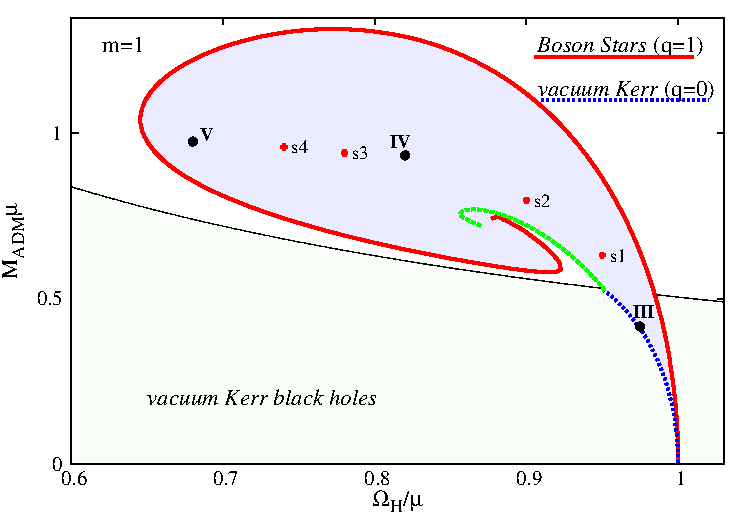
\includegraphics[scale=0.7]{figures/existence-eps-converted-to.pdf}
\caption{Domain of existence for KBHsSH in an ADM mass versus scalar
field frequency diagram. \tf{The figure has to be redone to label the 7 models used in this work.}}
\label{existence}
\end{figure}


\begin{figure*}
\centering
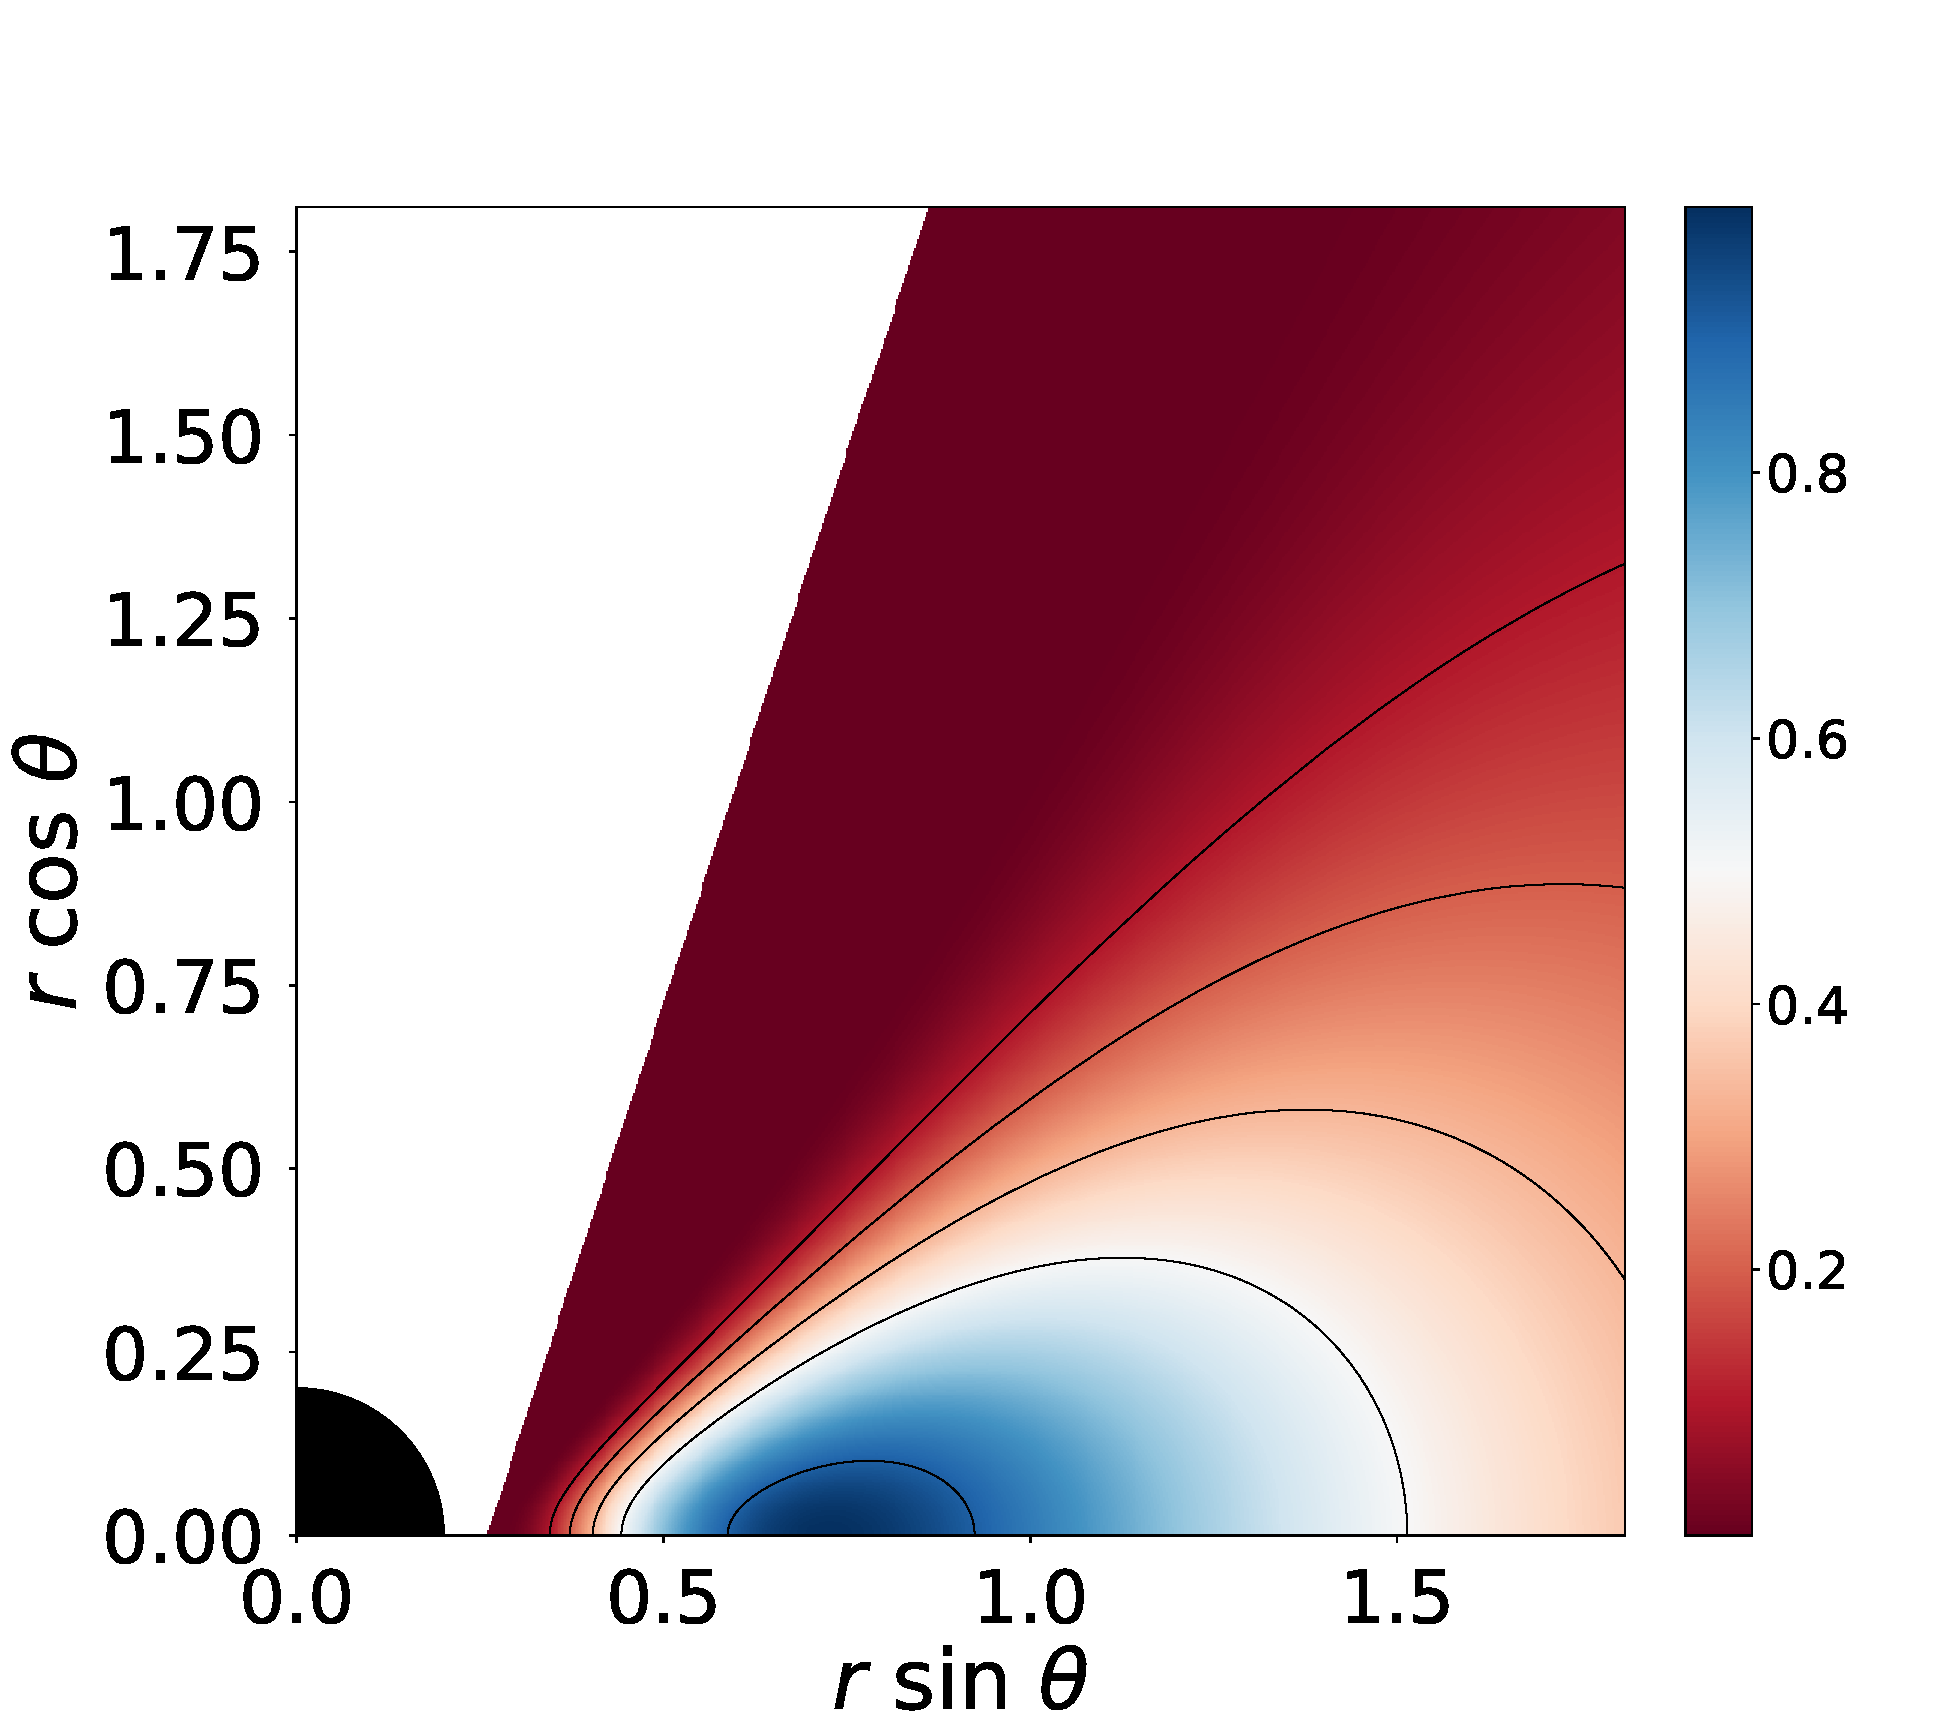
\includegraphics[scale=0.14]{figures/fig1_I_10.pdf}
\hspace{-0.3cm}
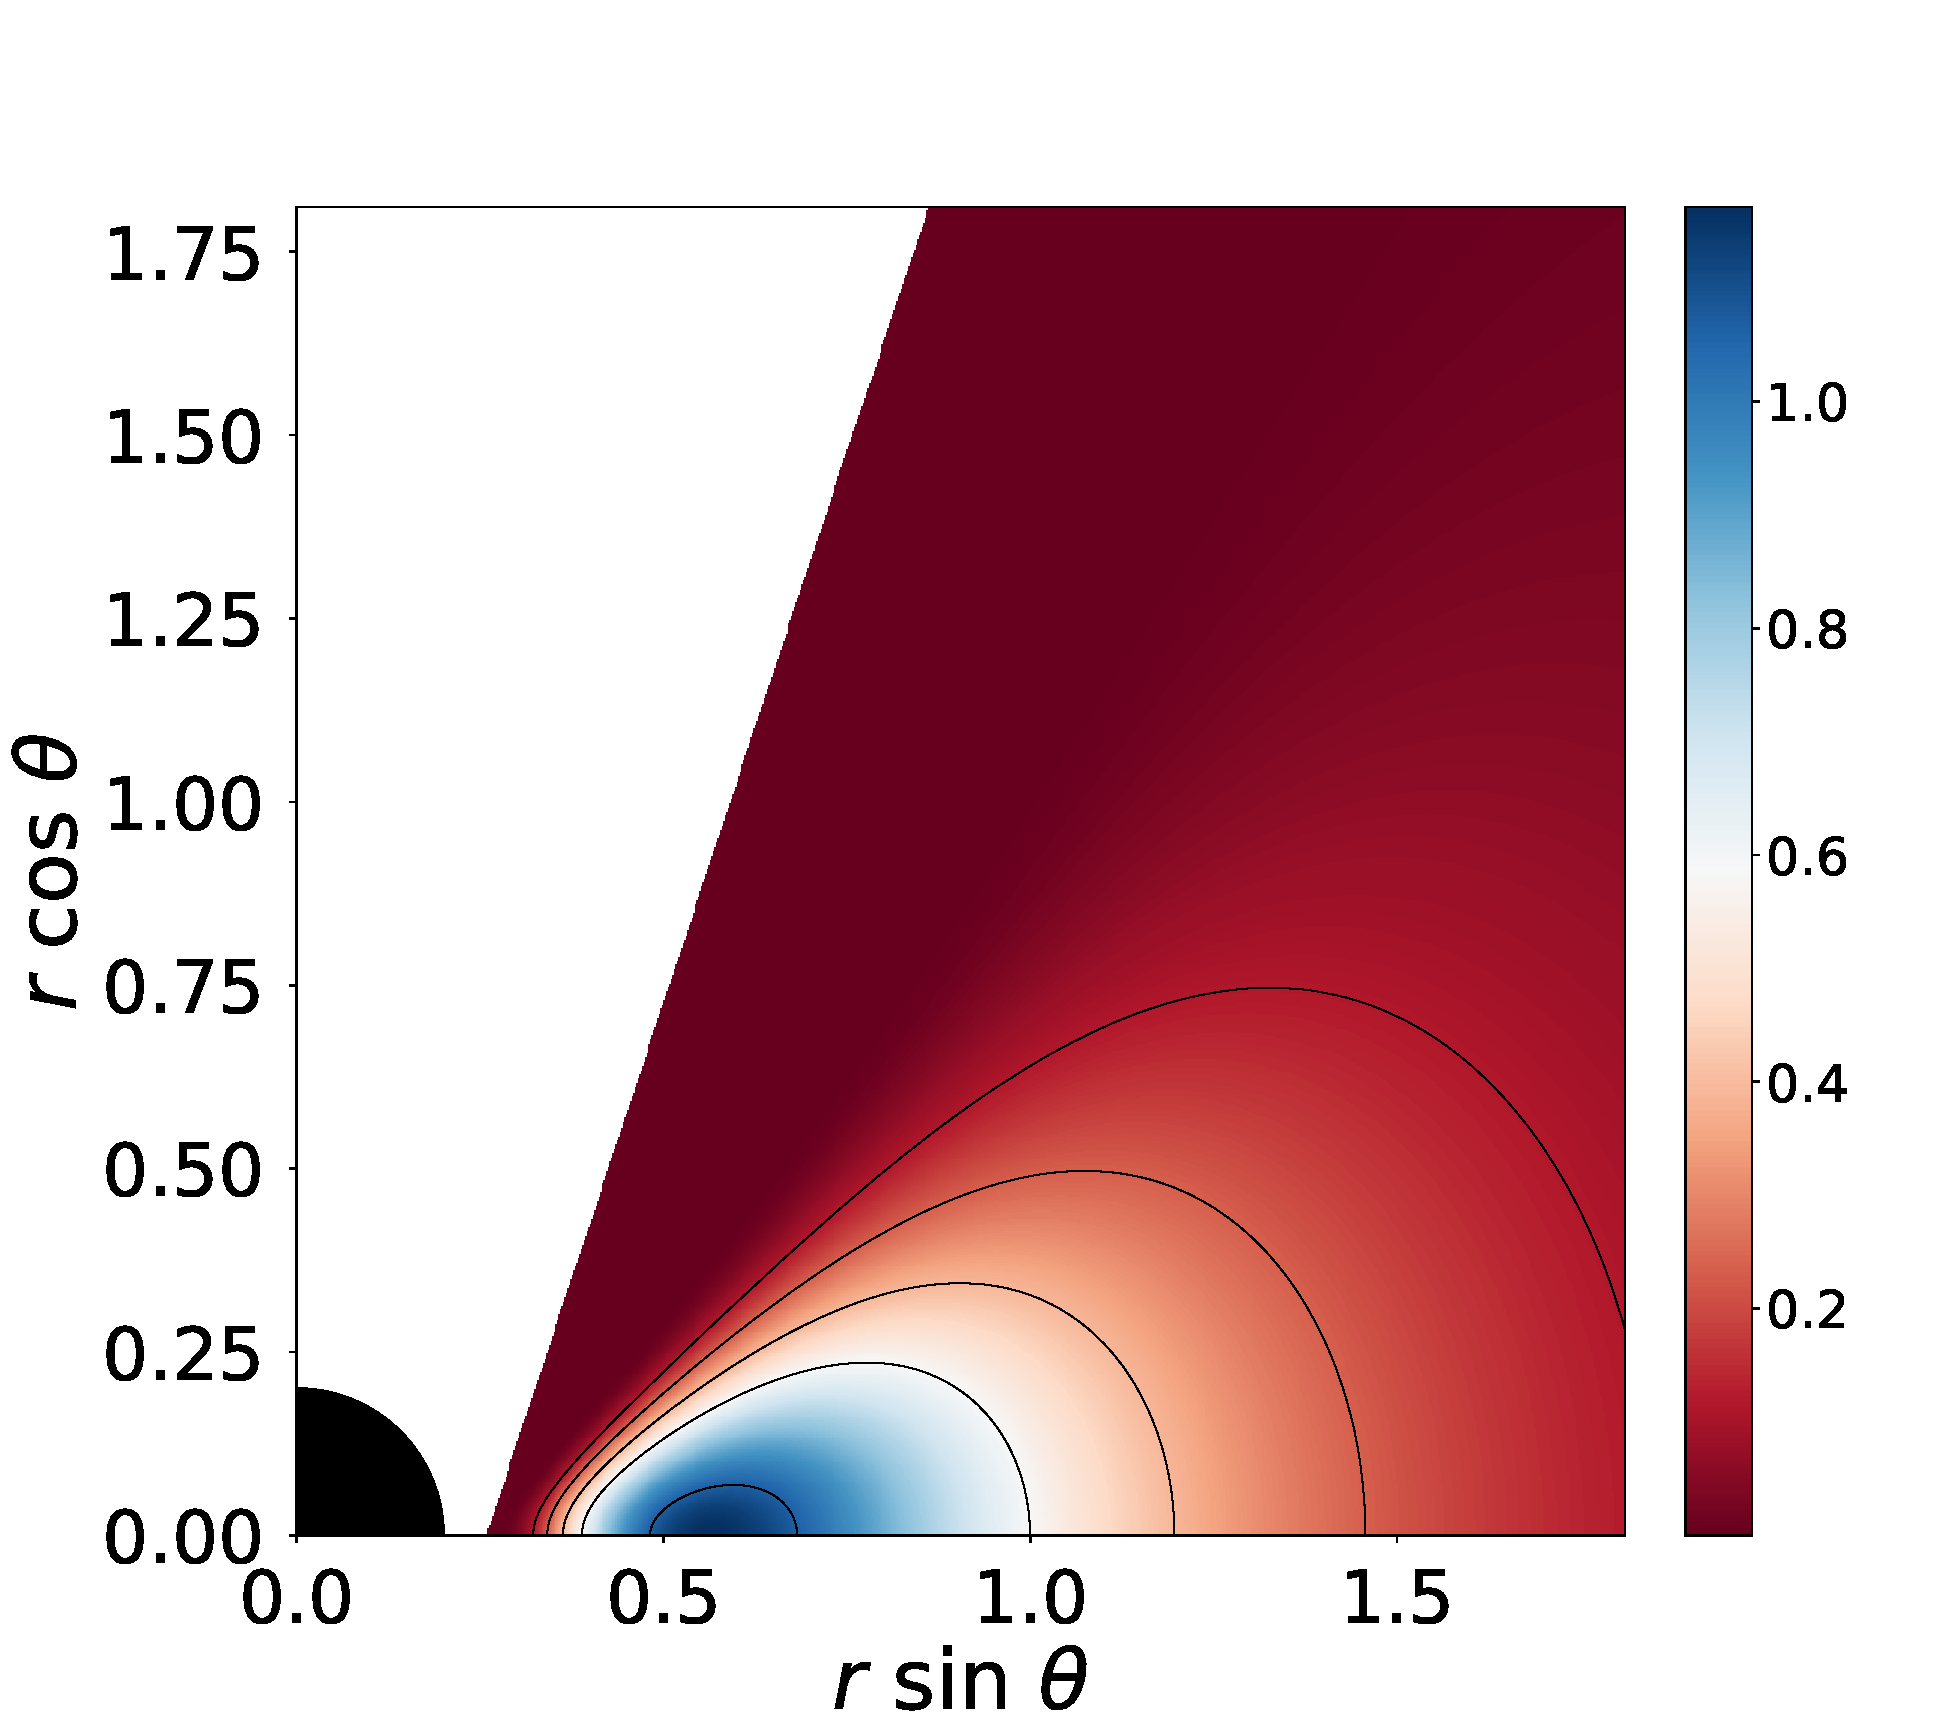
\includegraphics[scale=0.14]{figures/fig1_I_1.pdf}
\hspace{-0.2cm}
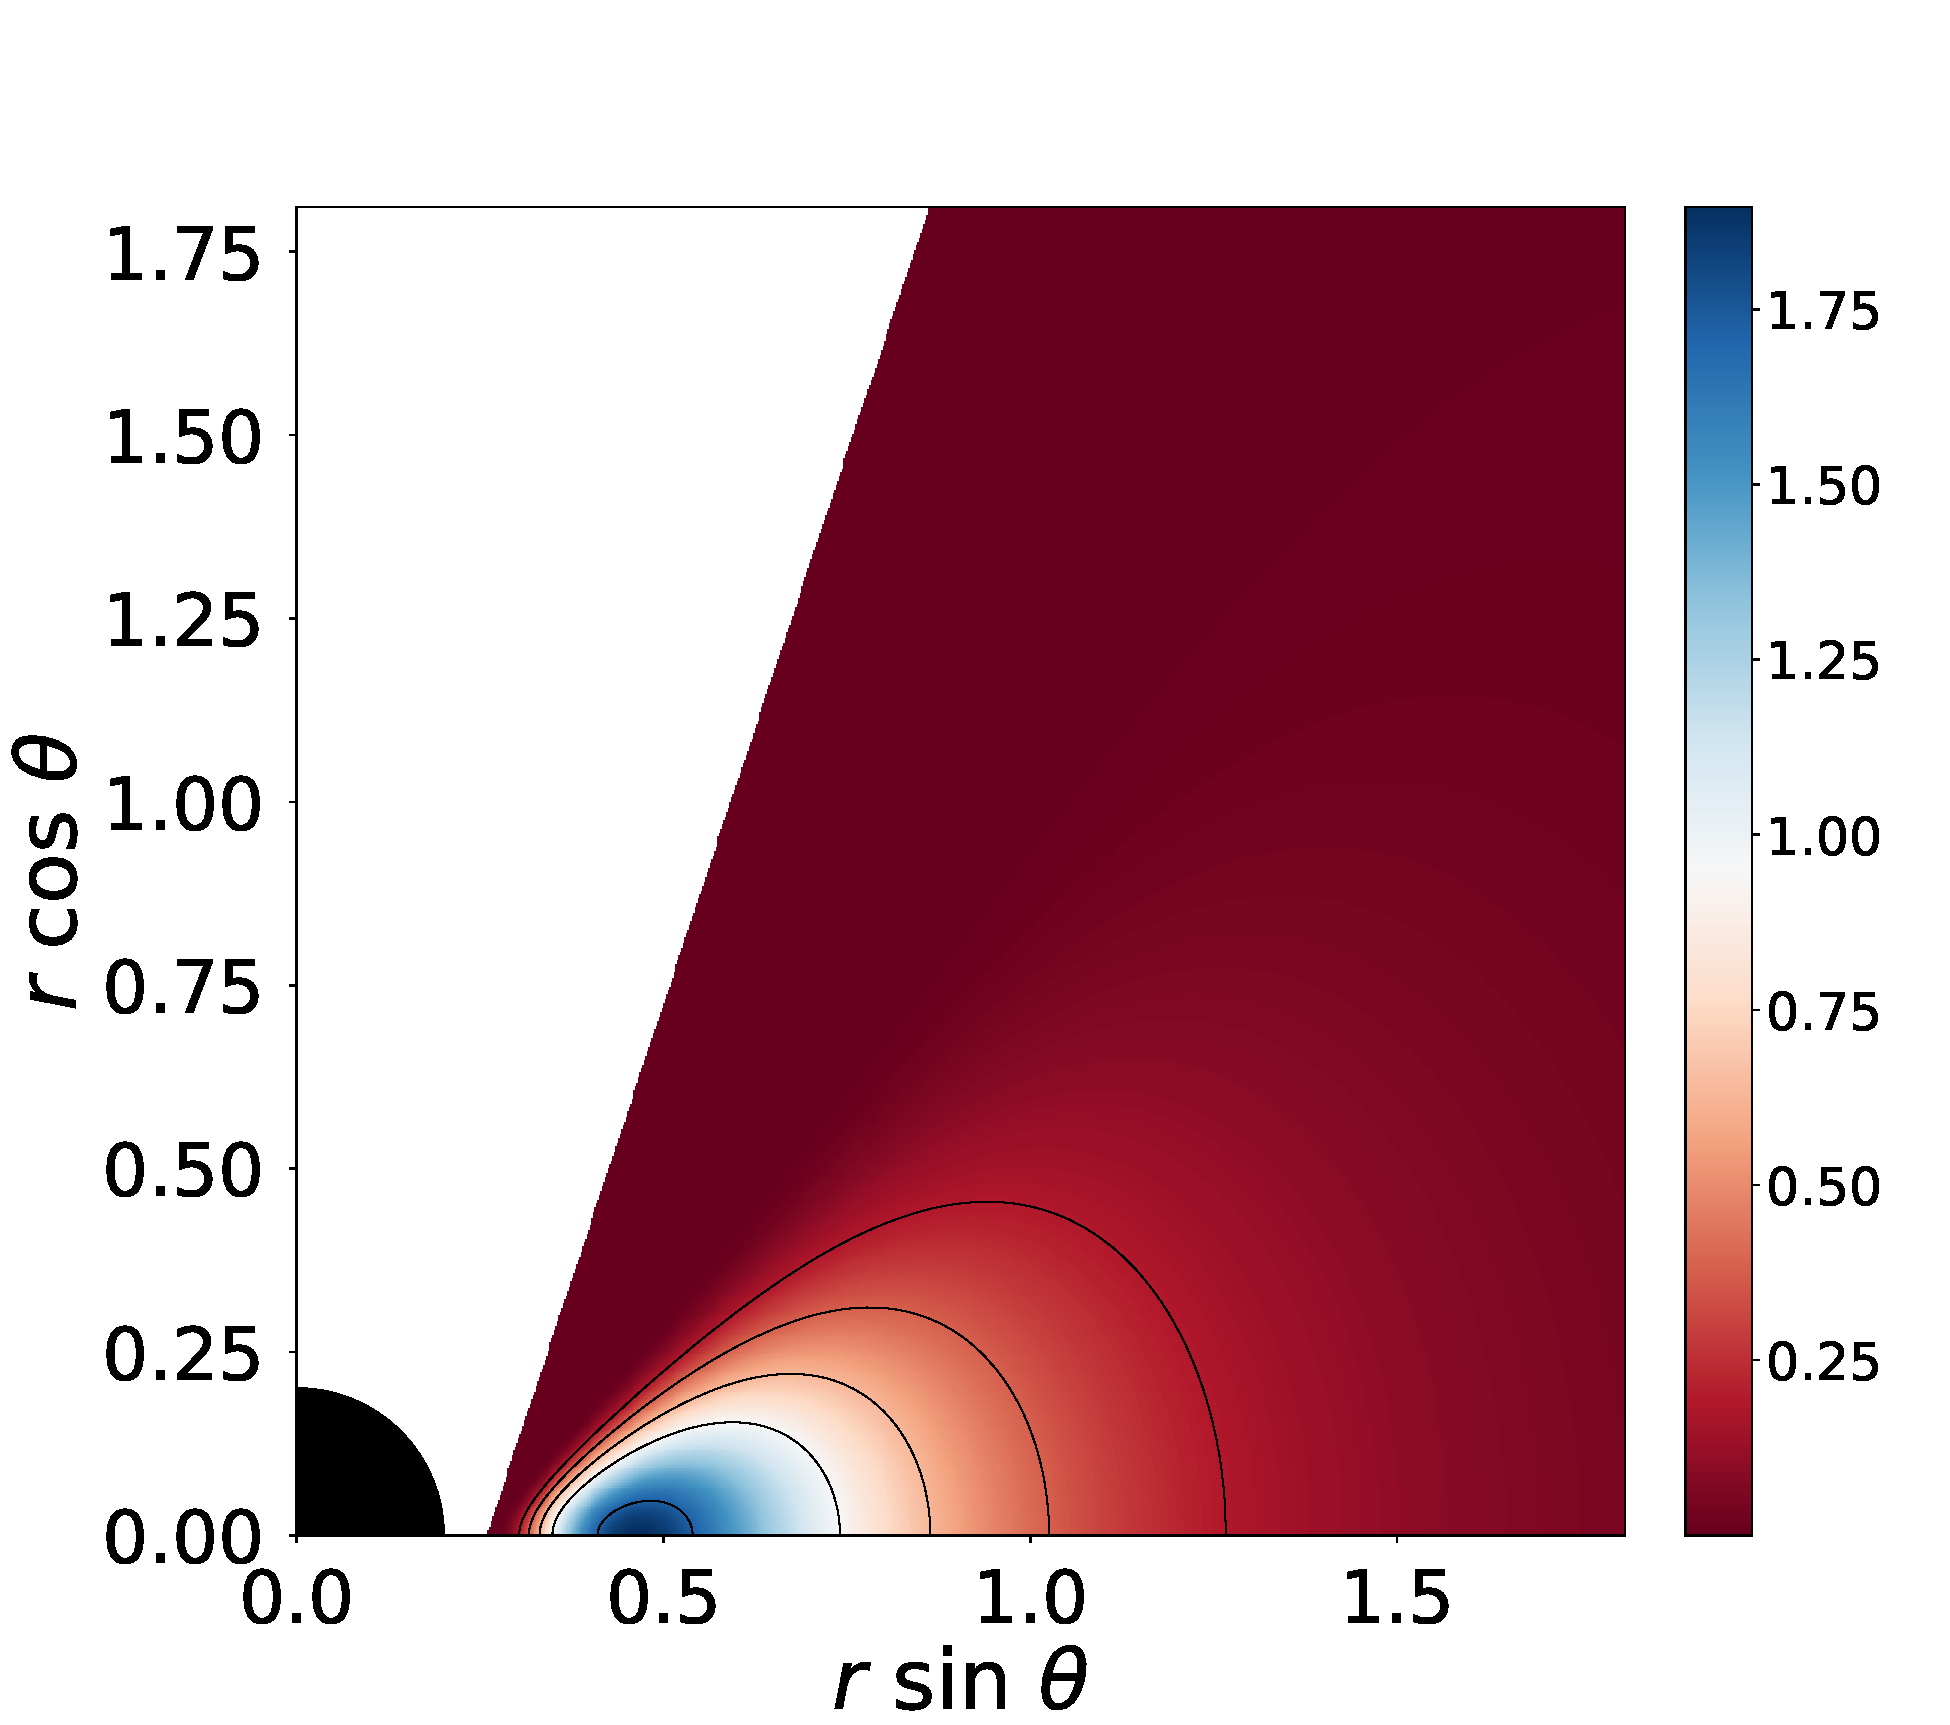
\includegraphics[scale=0.14]{figures/fig1_I__10.pdf}
\\
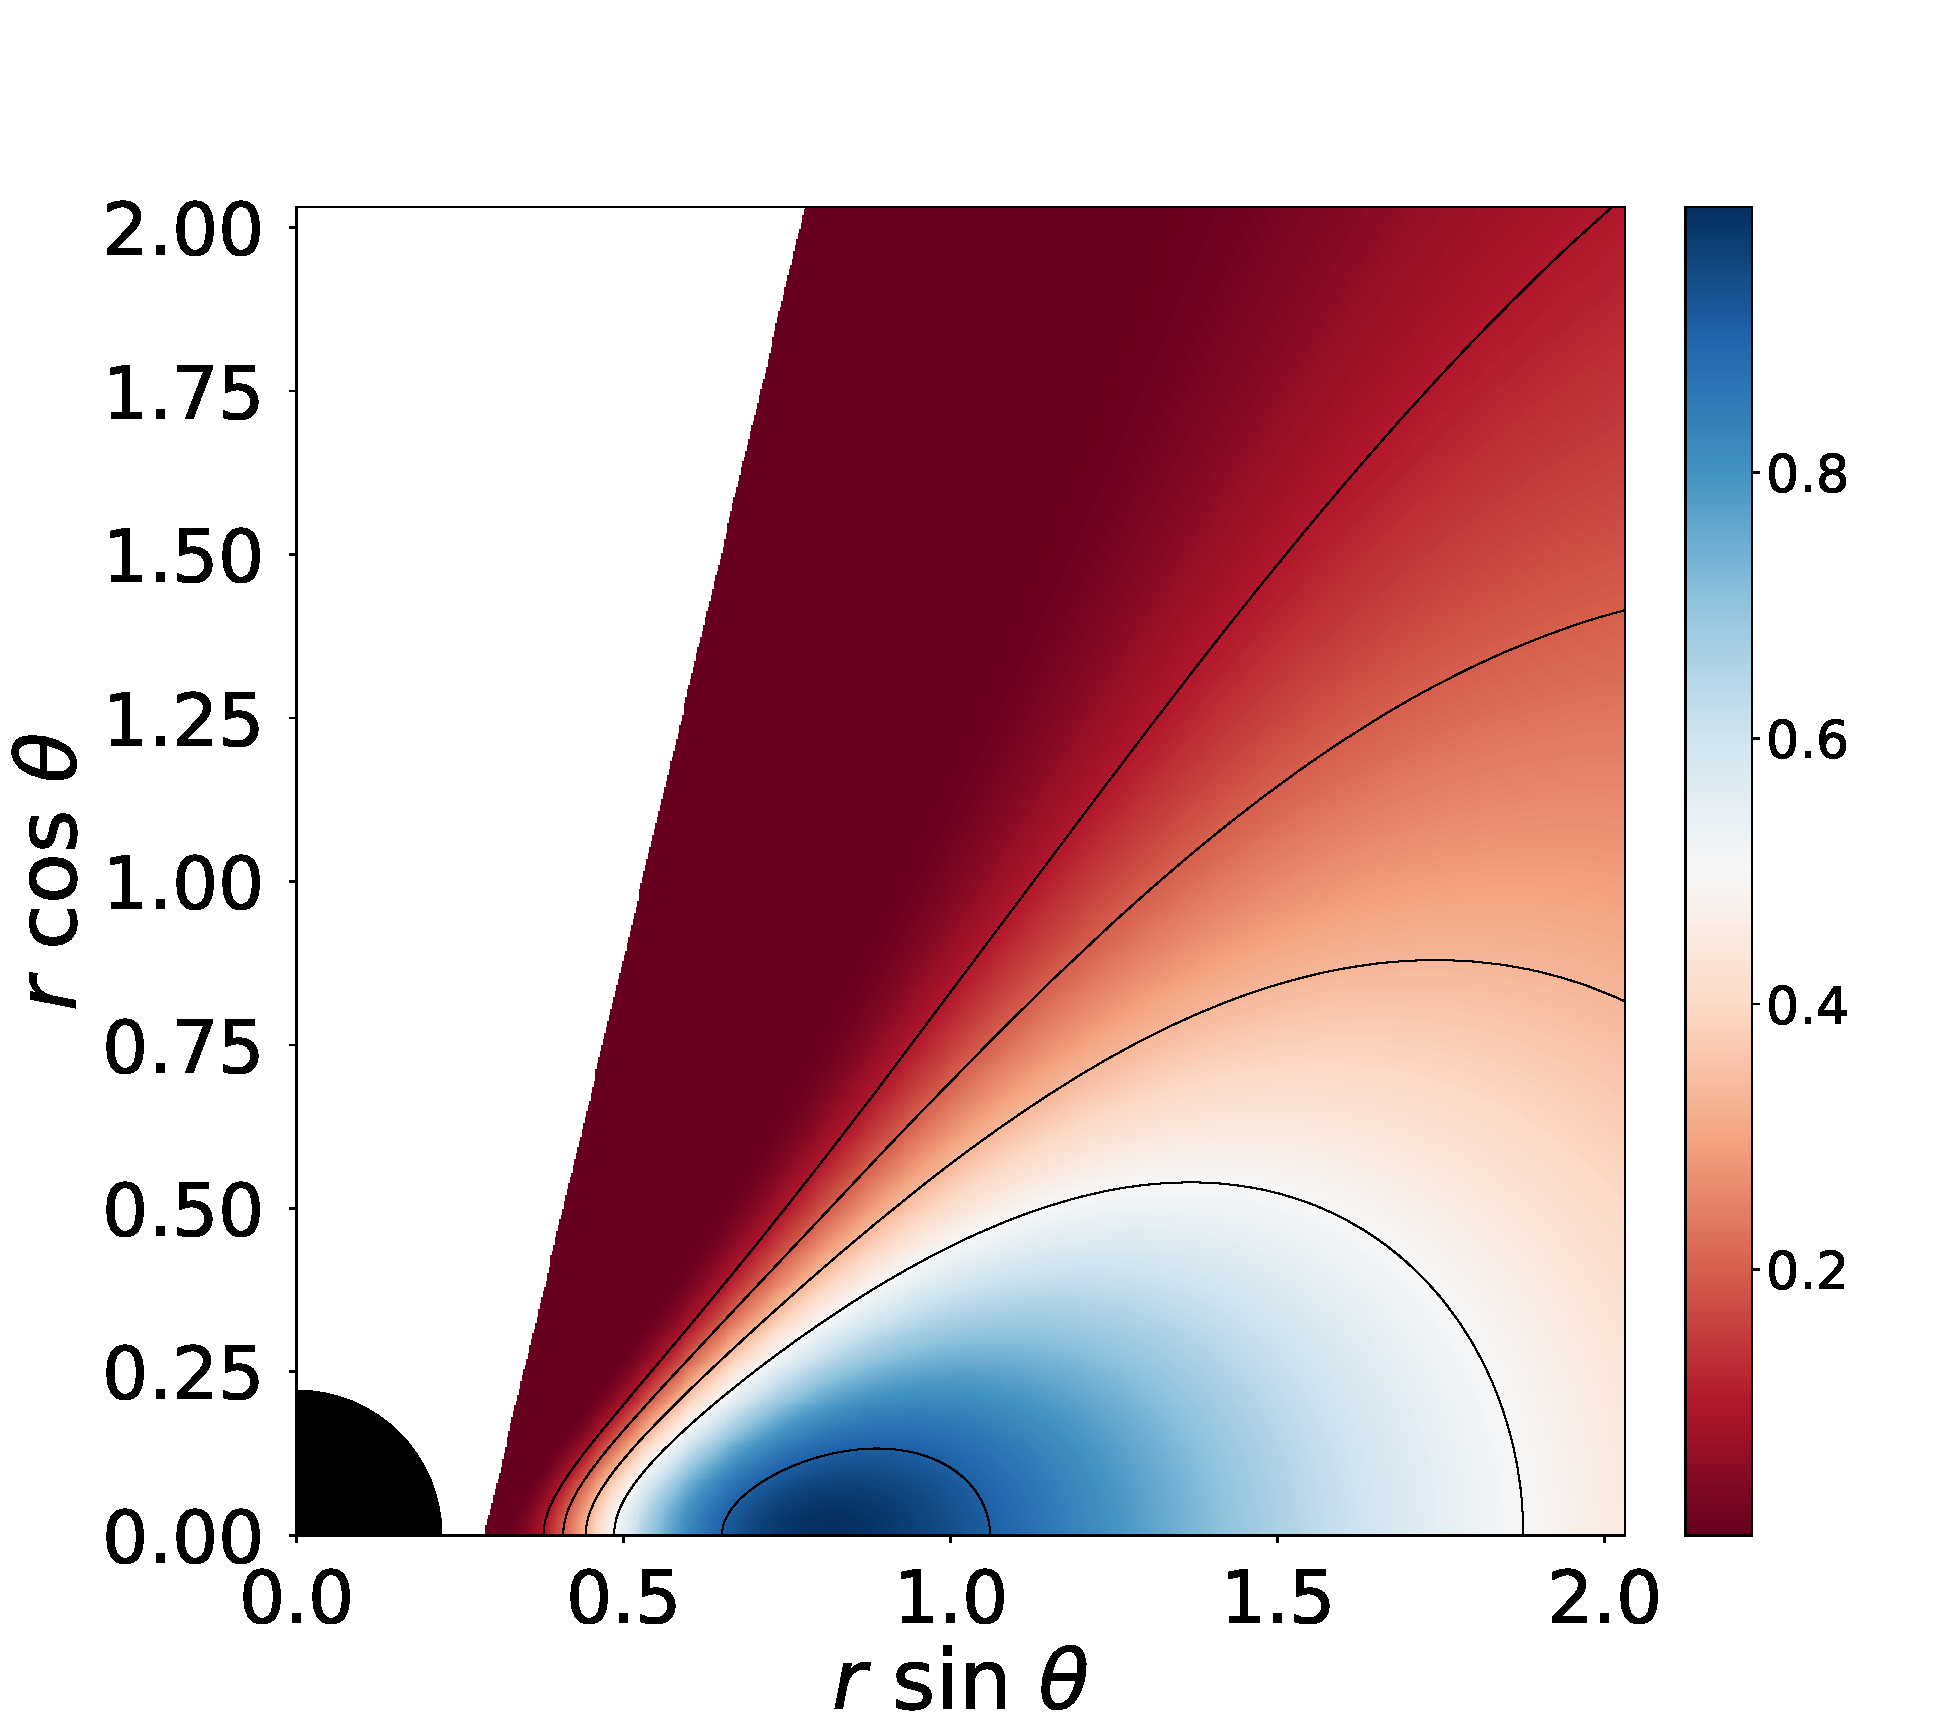
\includegraphics[scale=0.14]{figures/fig1_II_10.pdf}
\hspace{-0.3cm}
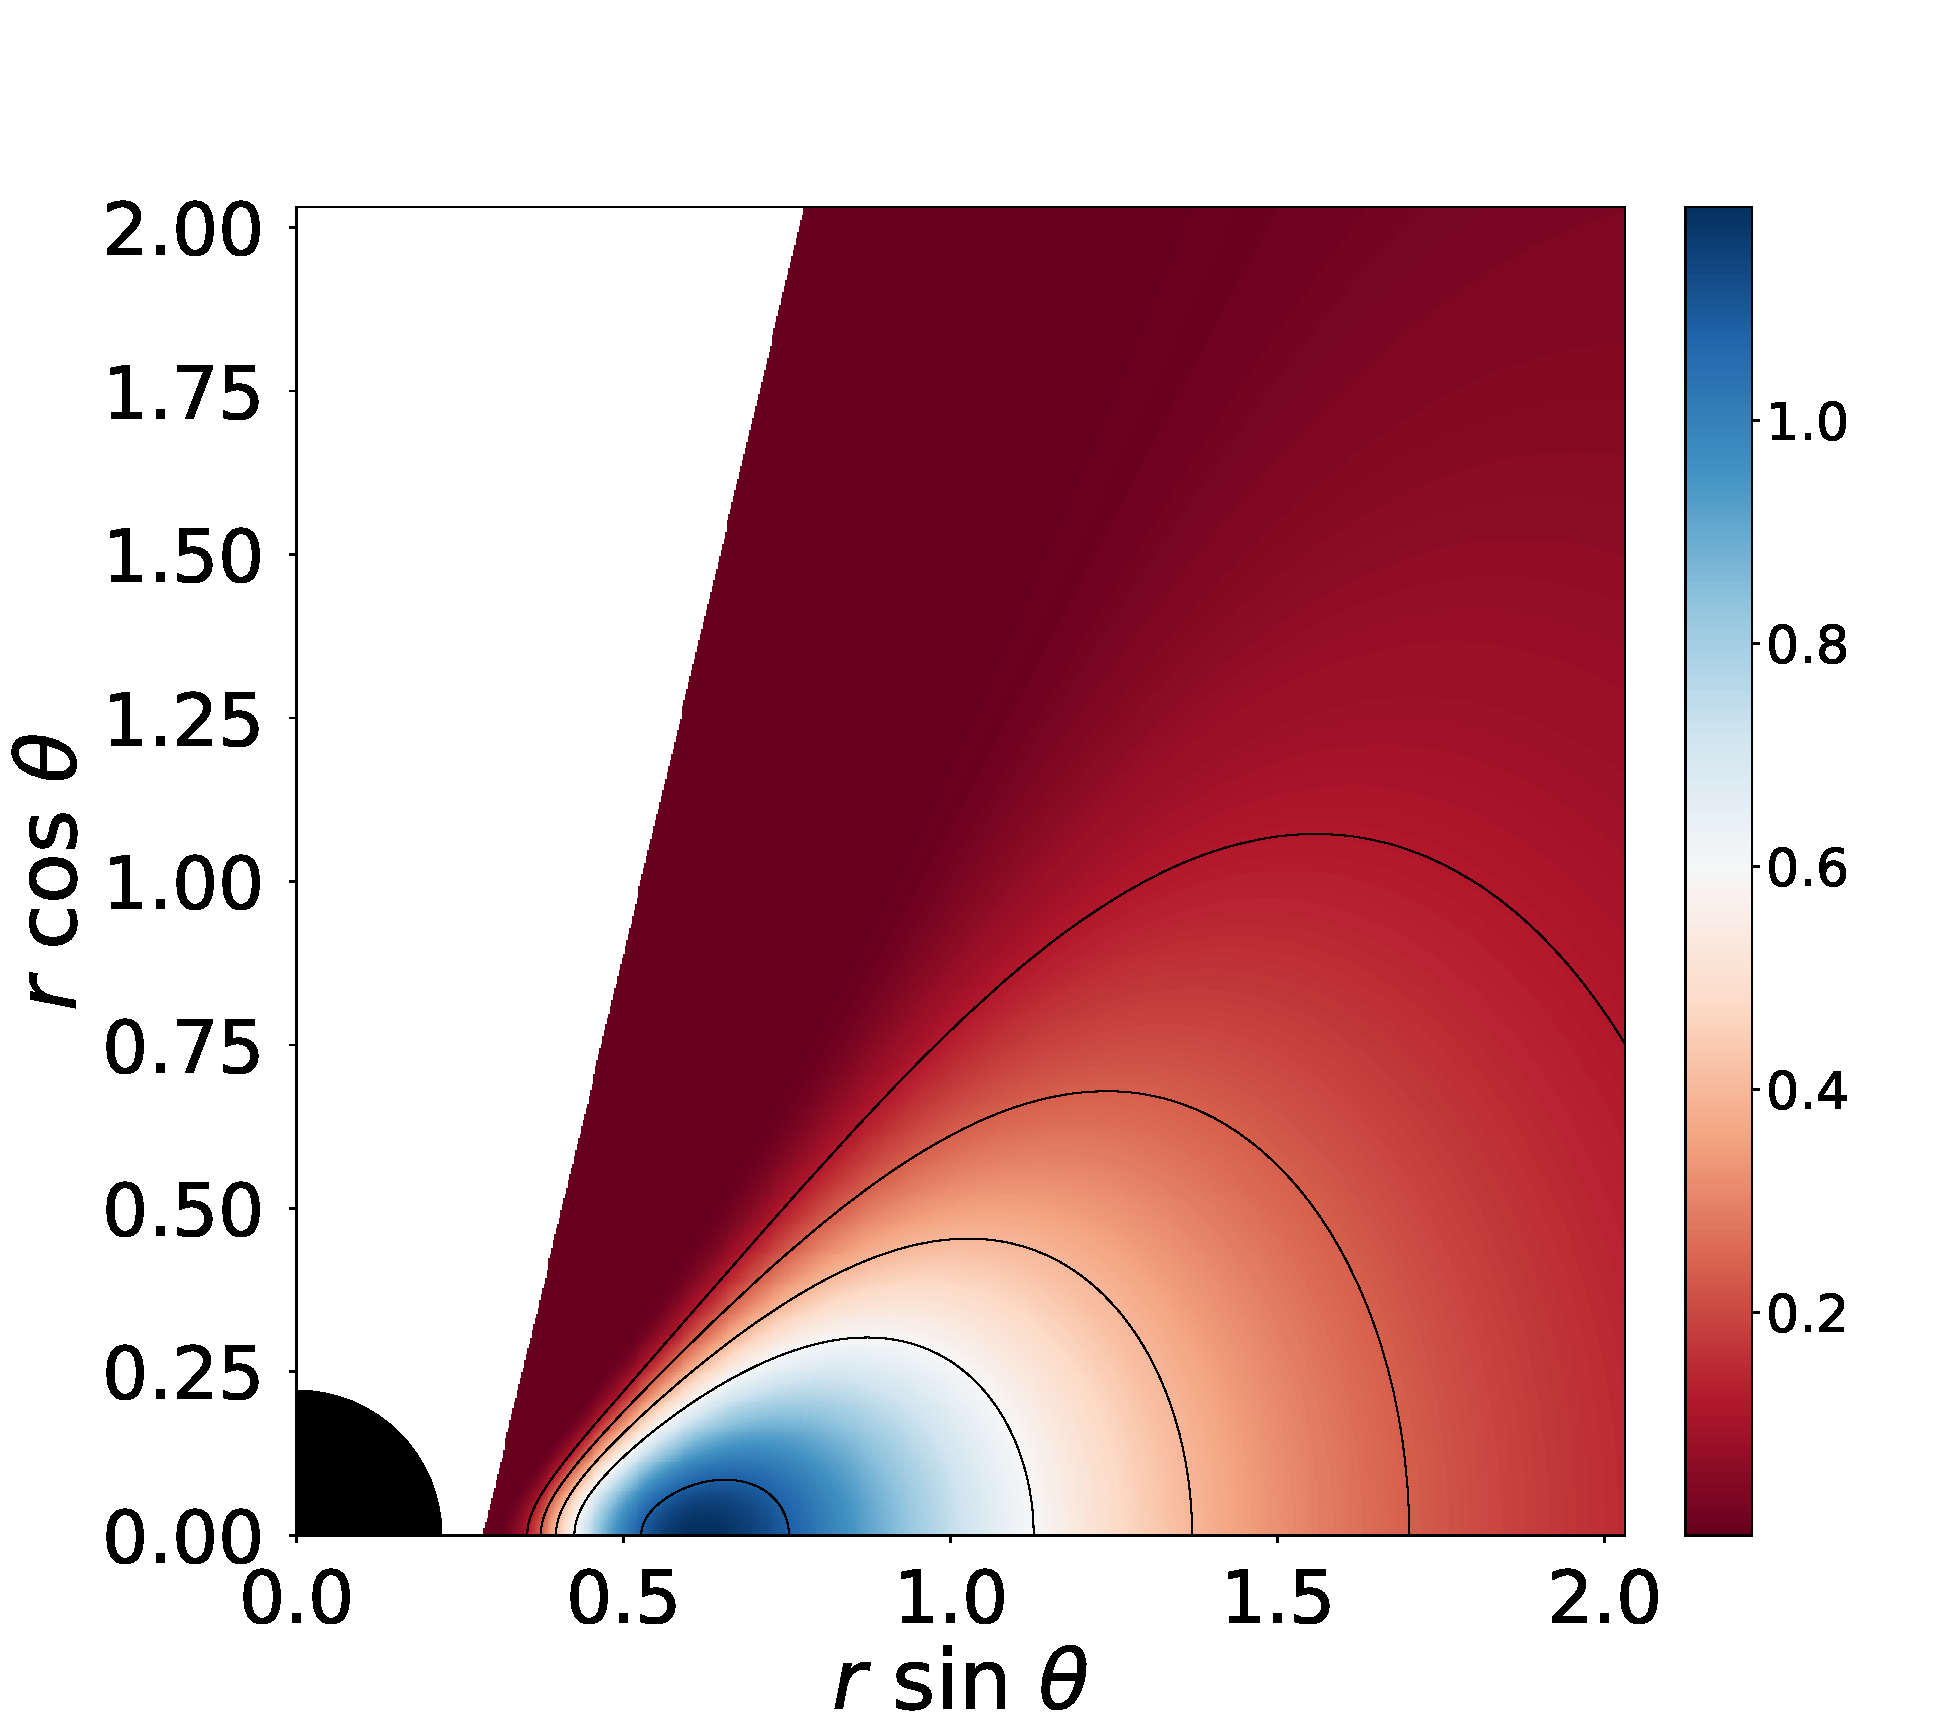
\includegraphics[scale=0.14]{figures/fig1_II_1.pdf}
\hspace{-0.2cm}
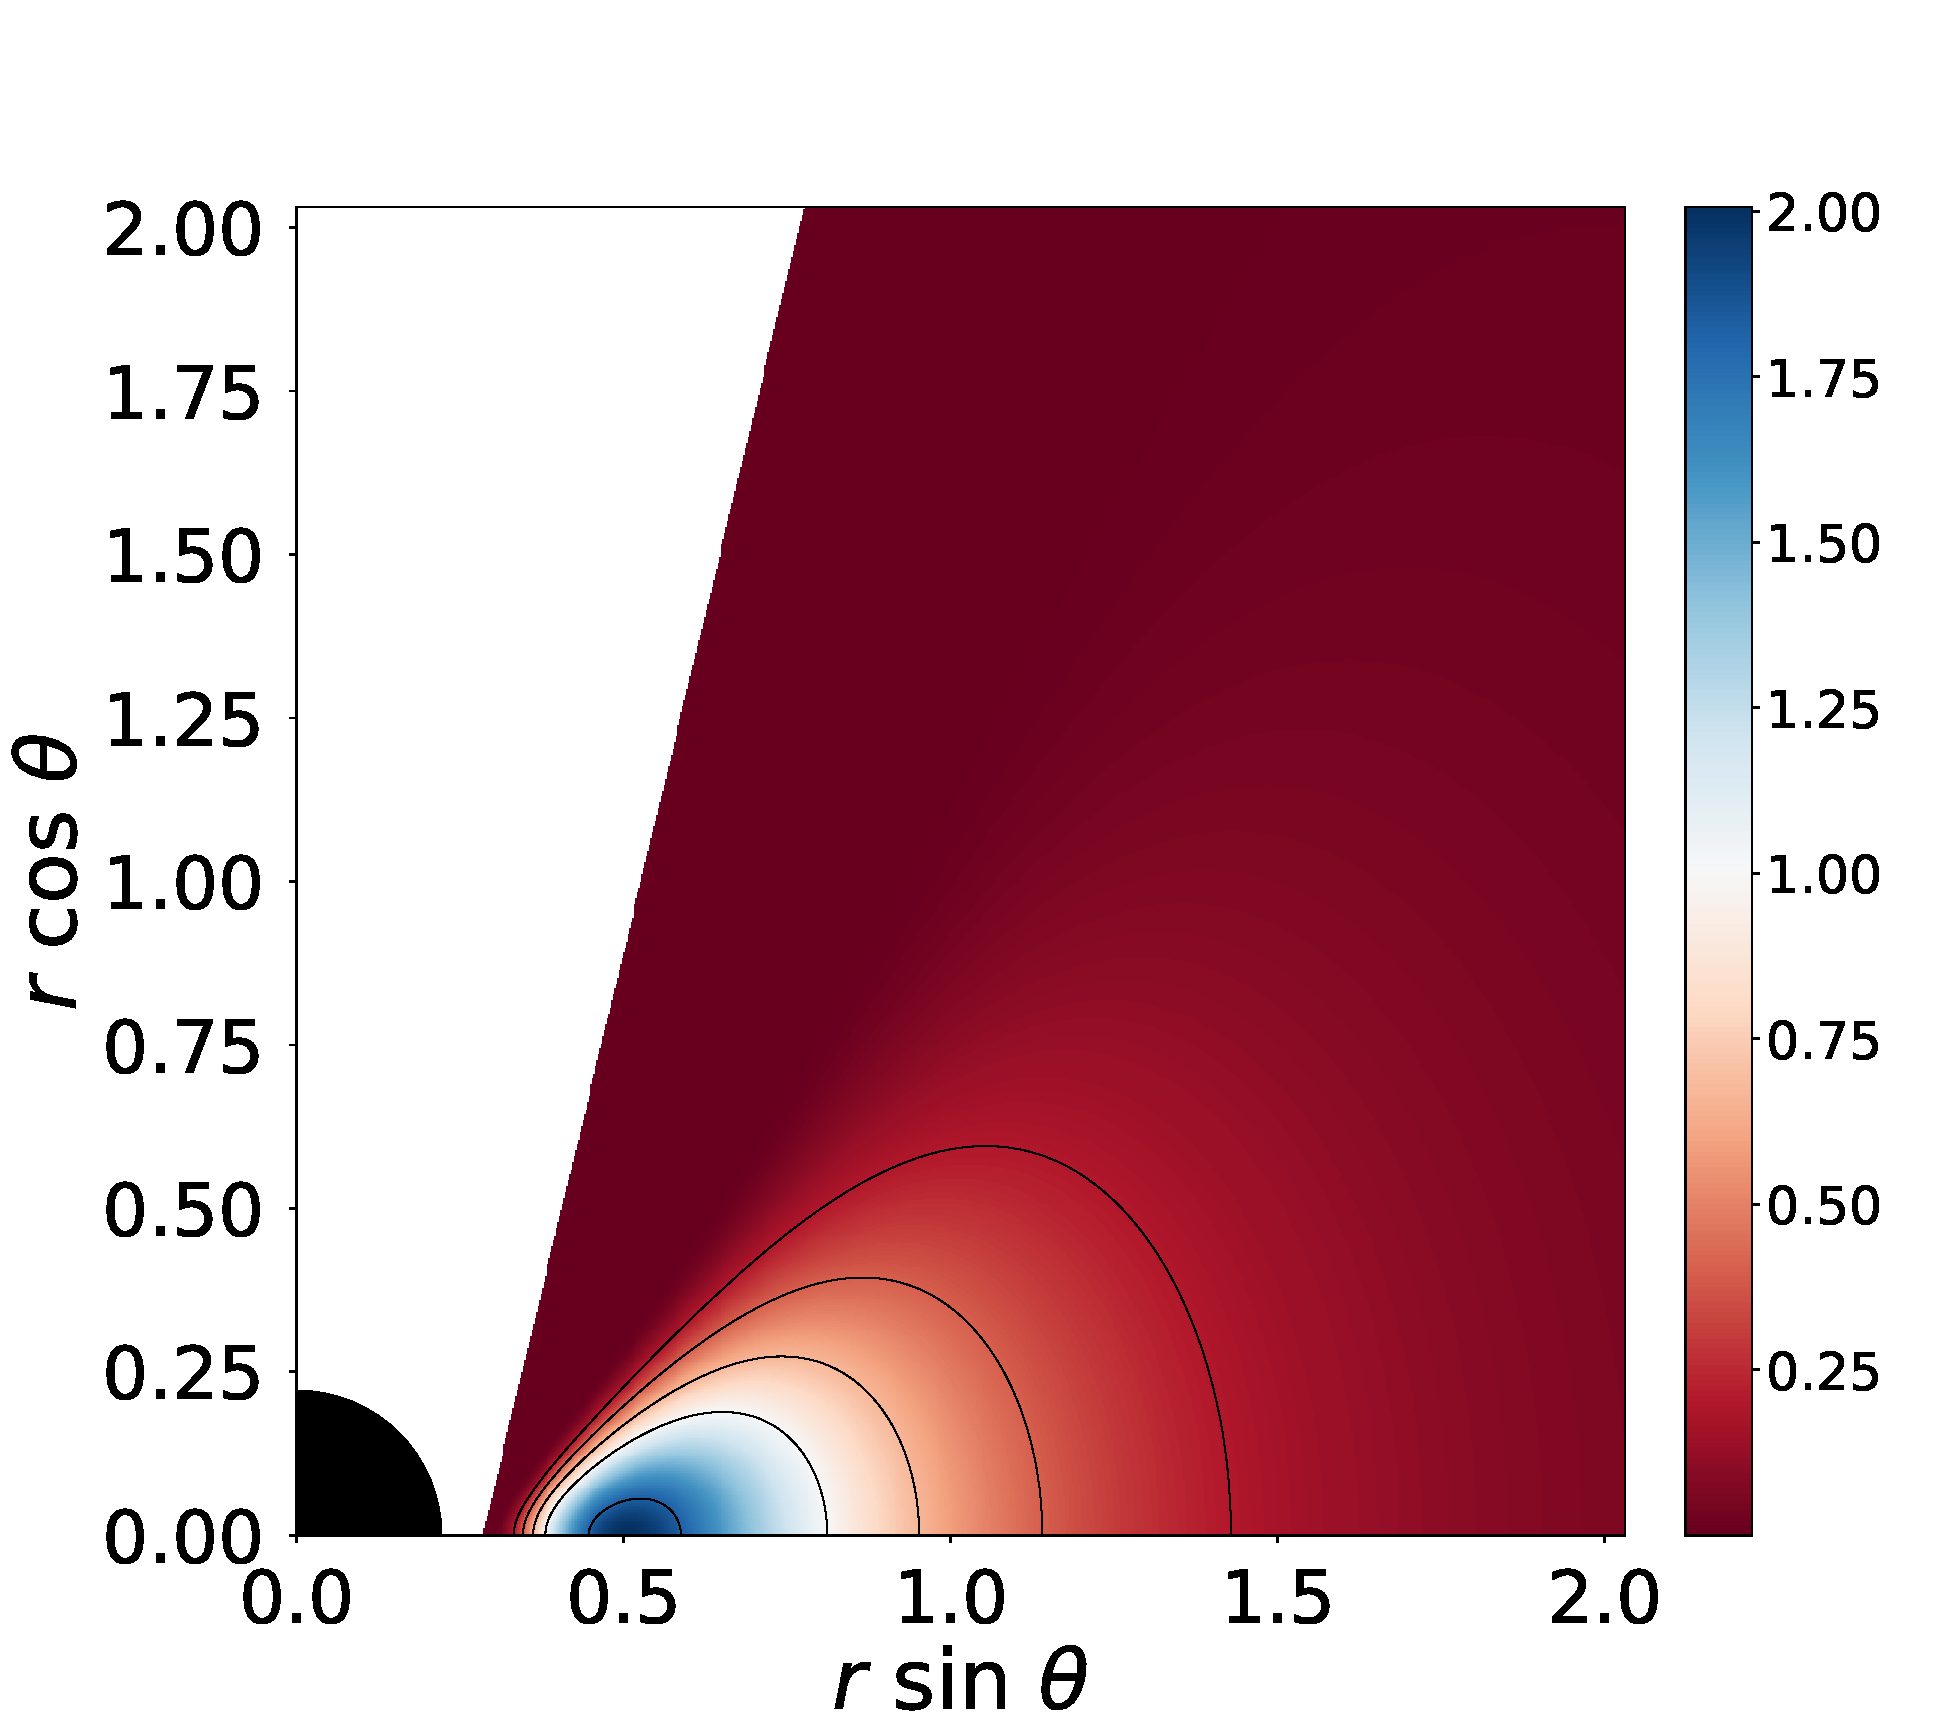
\includegraphics[scale=0.14]{figures/fig1_II__10.pdf}
\\
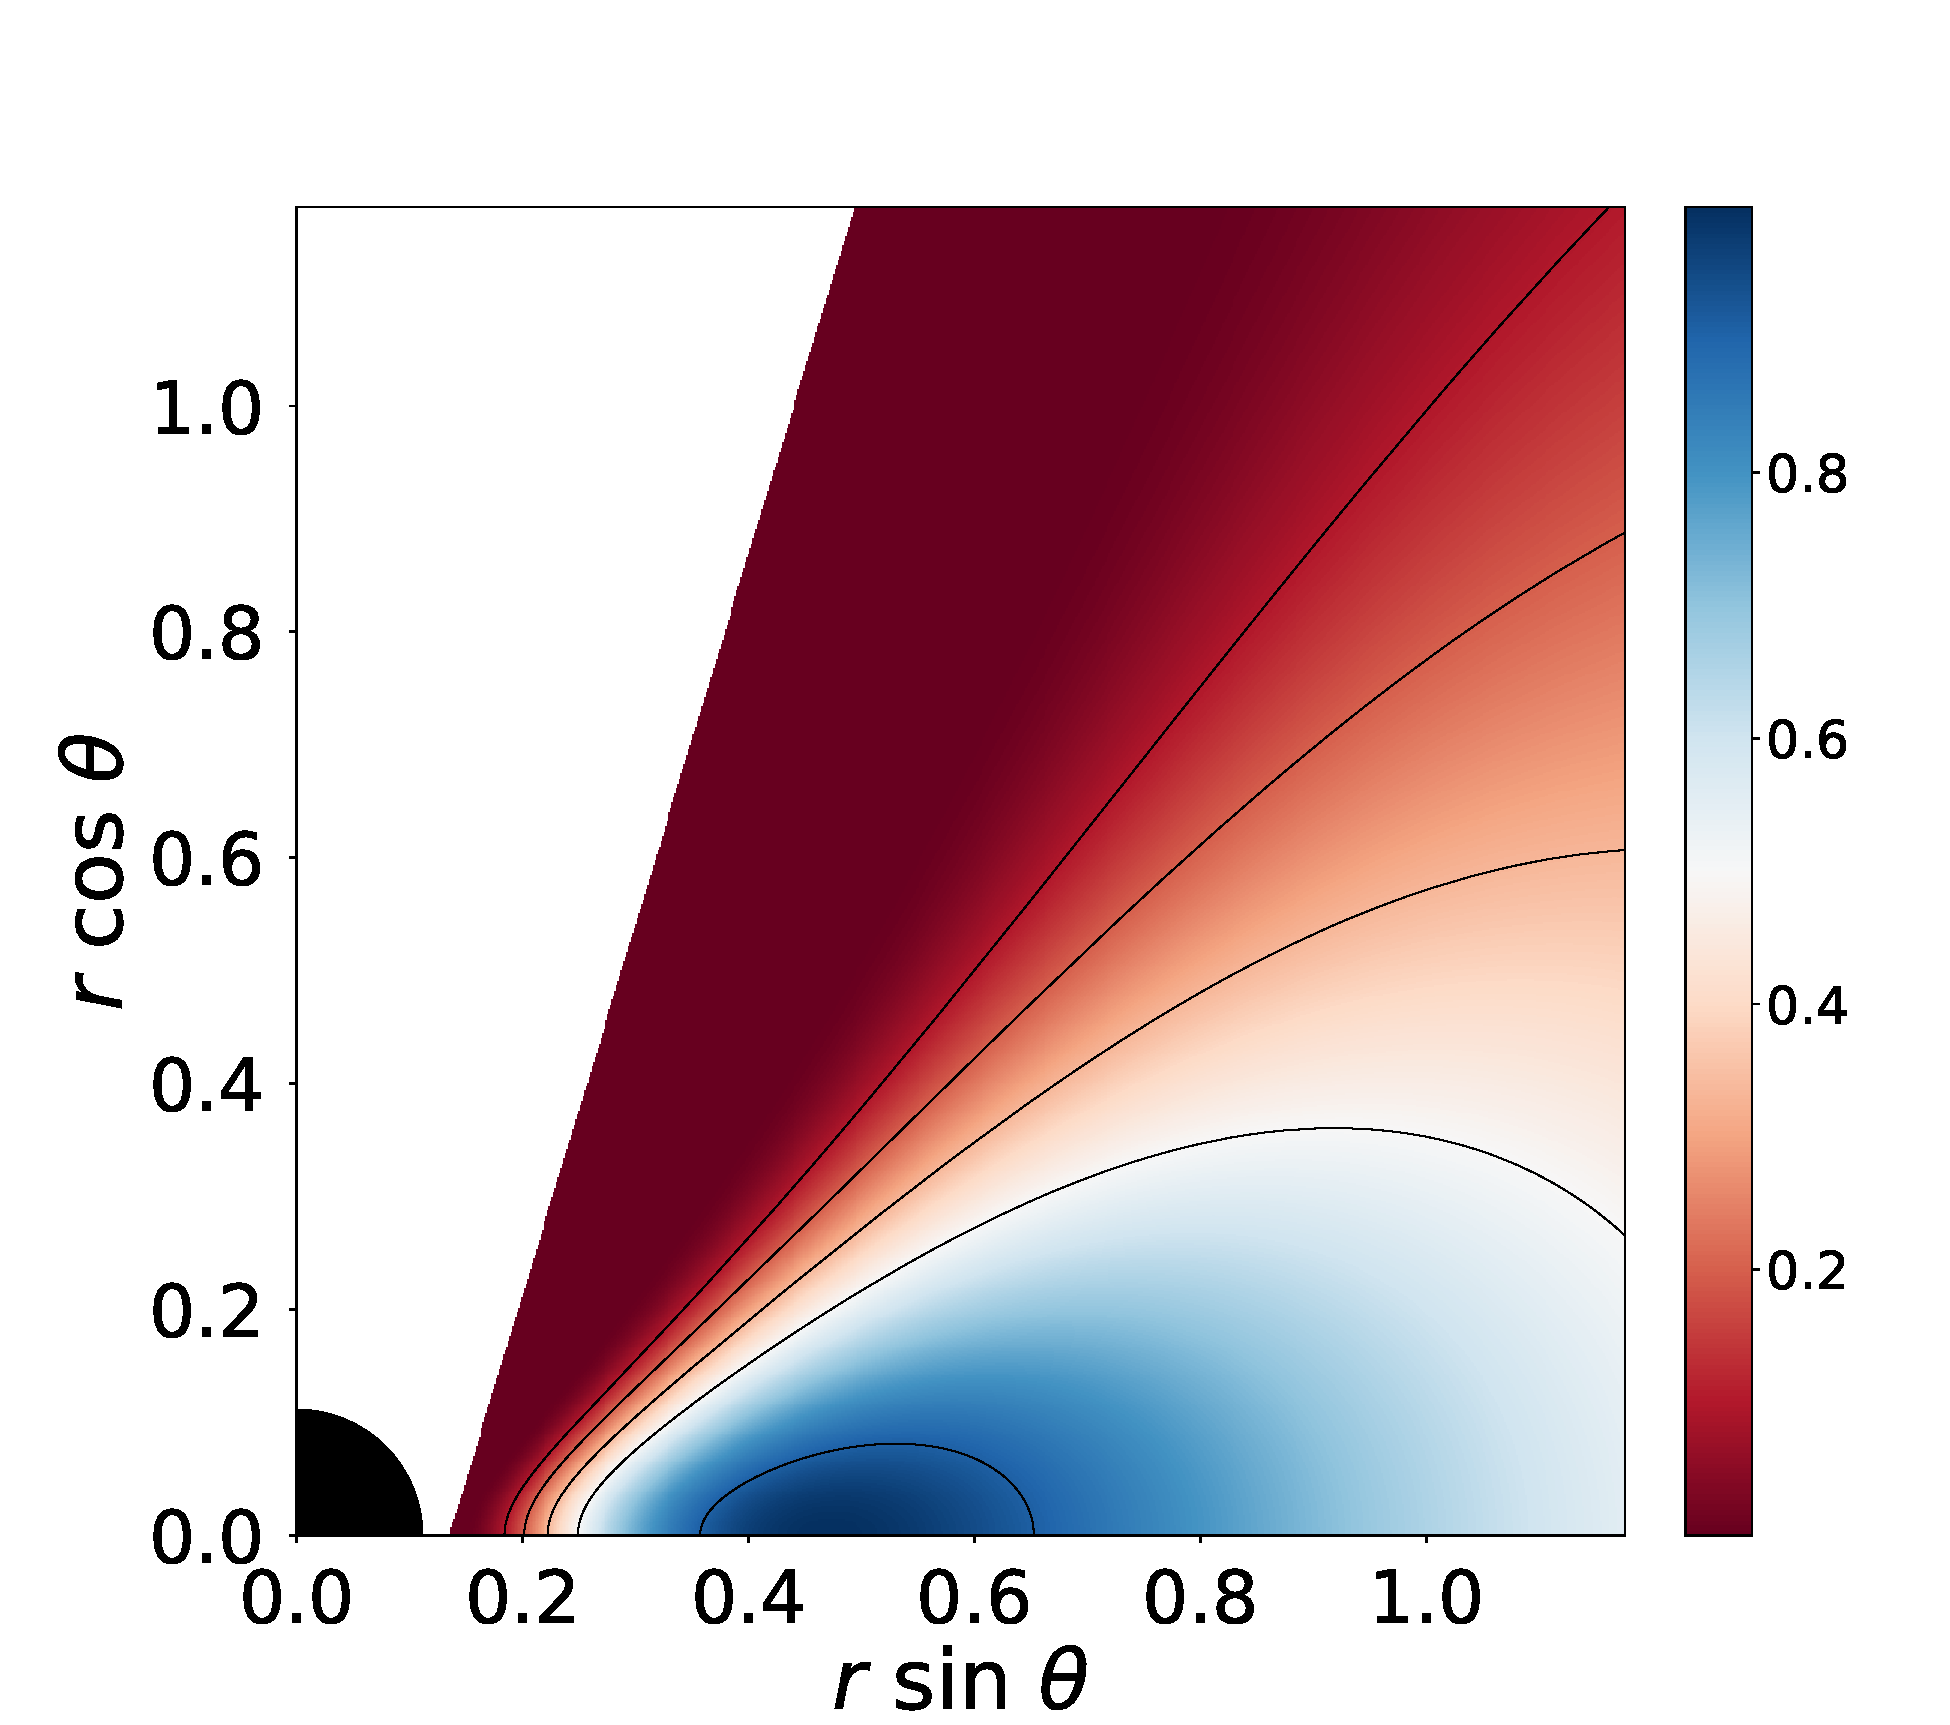
\includegraphics[scale=0.14]{figures/fig1_III_10.pdf}
\hspace{-0.3cm}
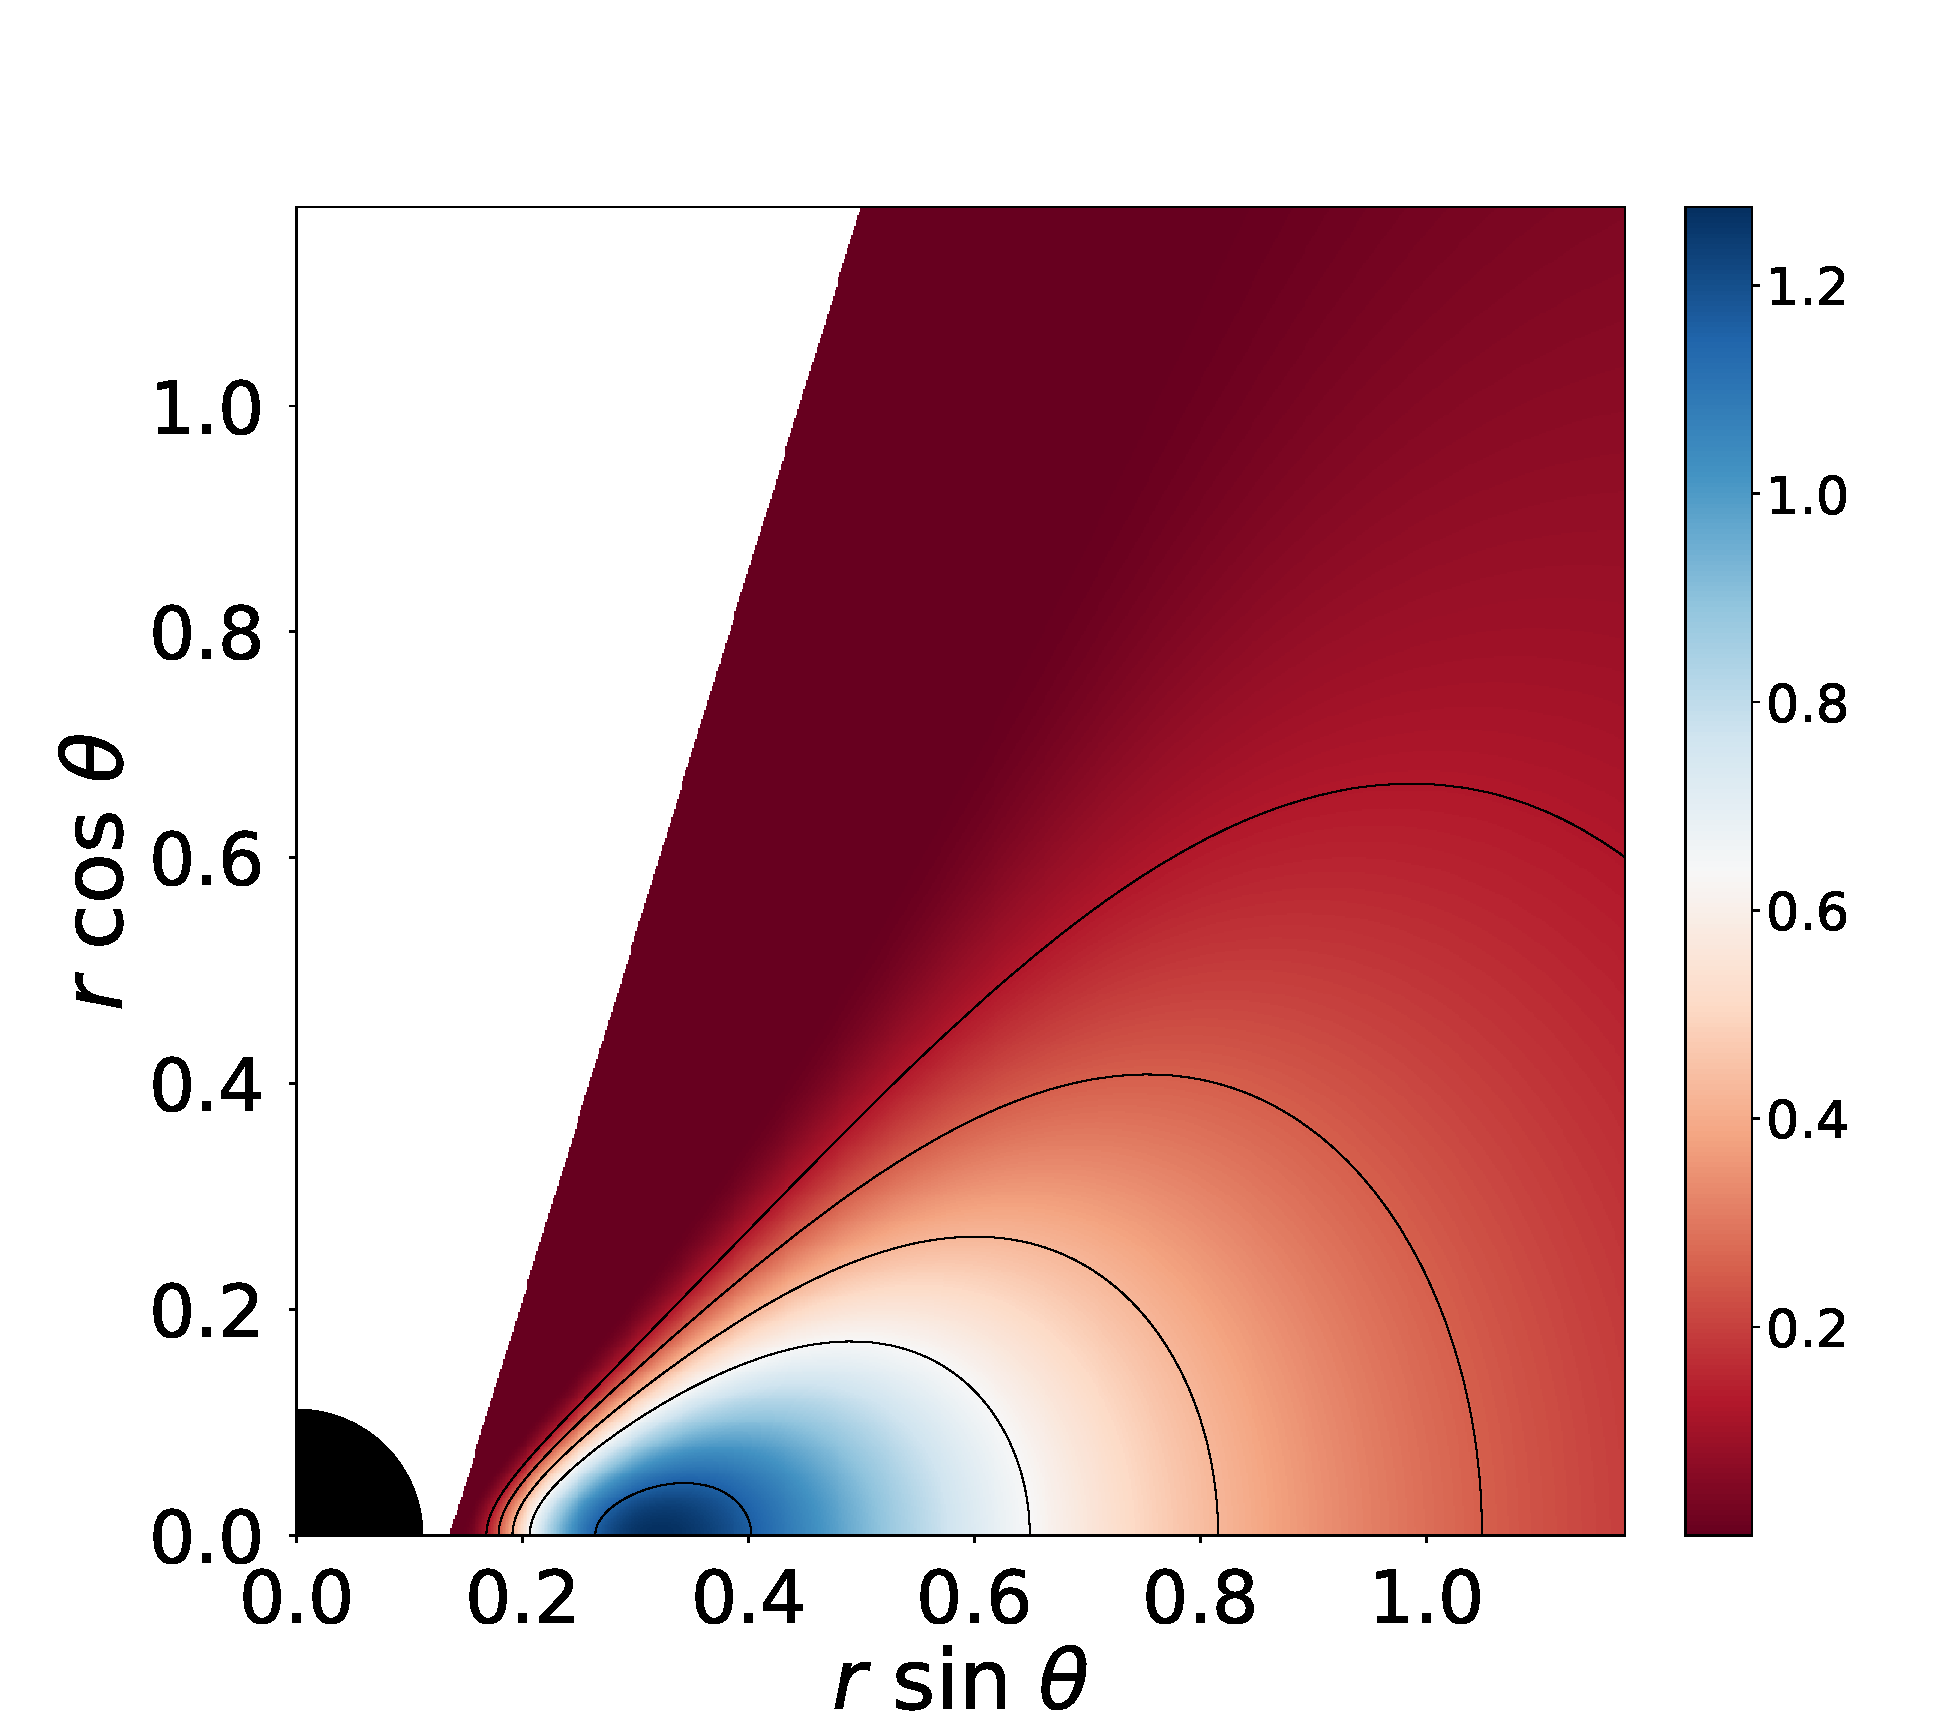
\includegraphics[scale=0.14]{figures/fig1_III_1.pdf}
\hspace{-0.2cm}
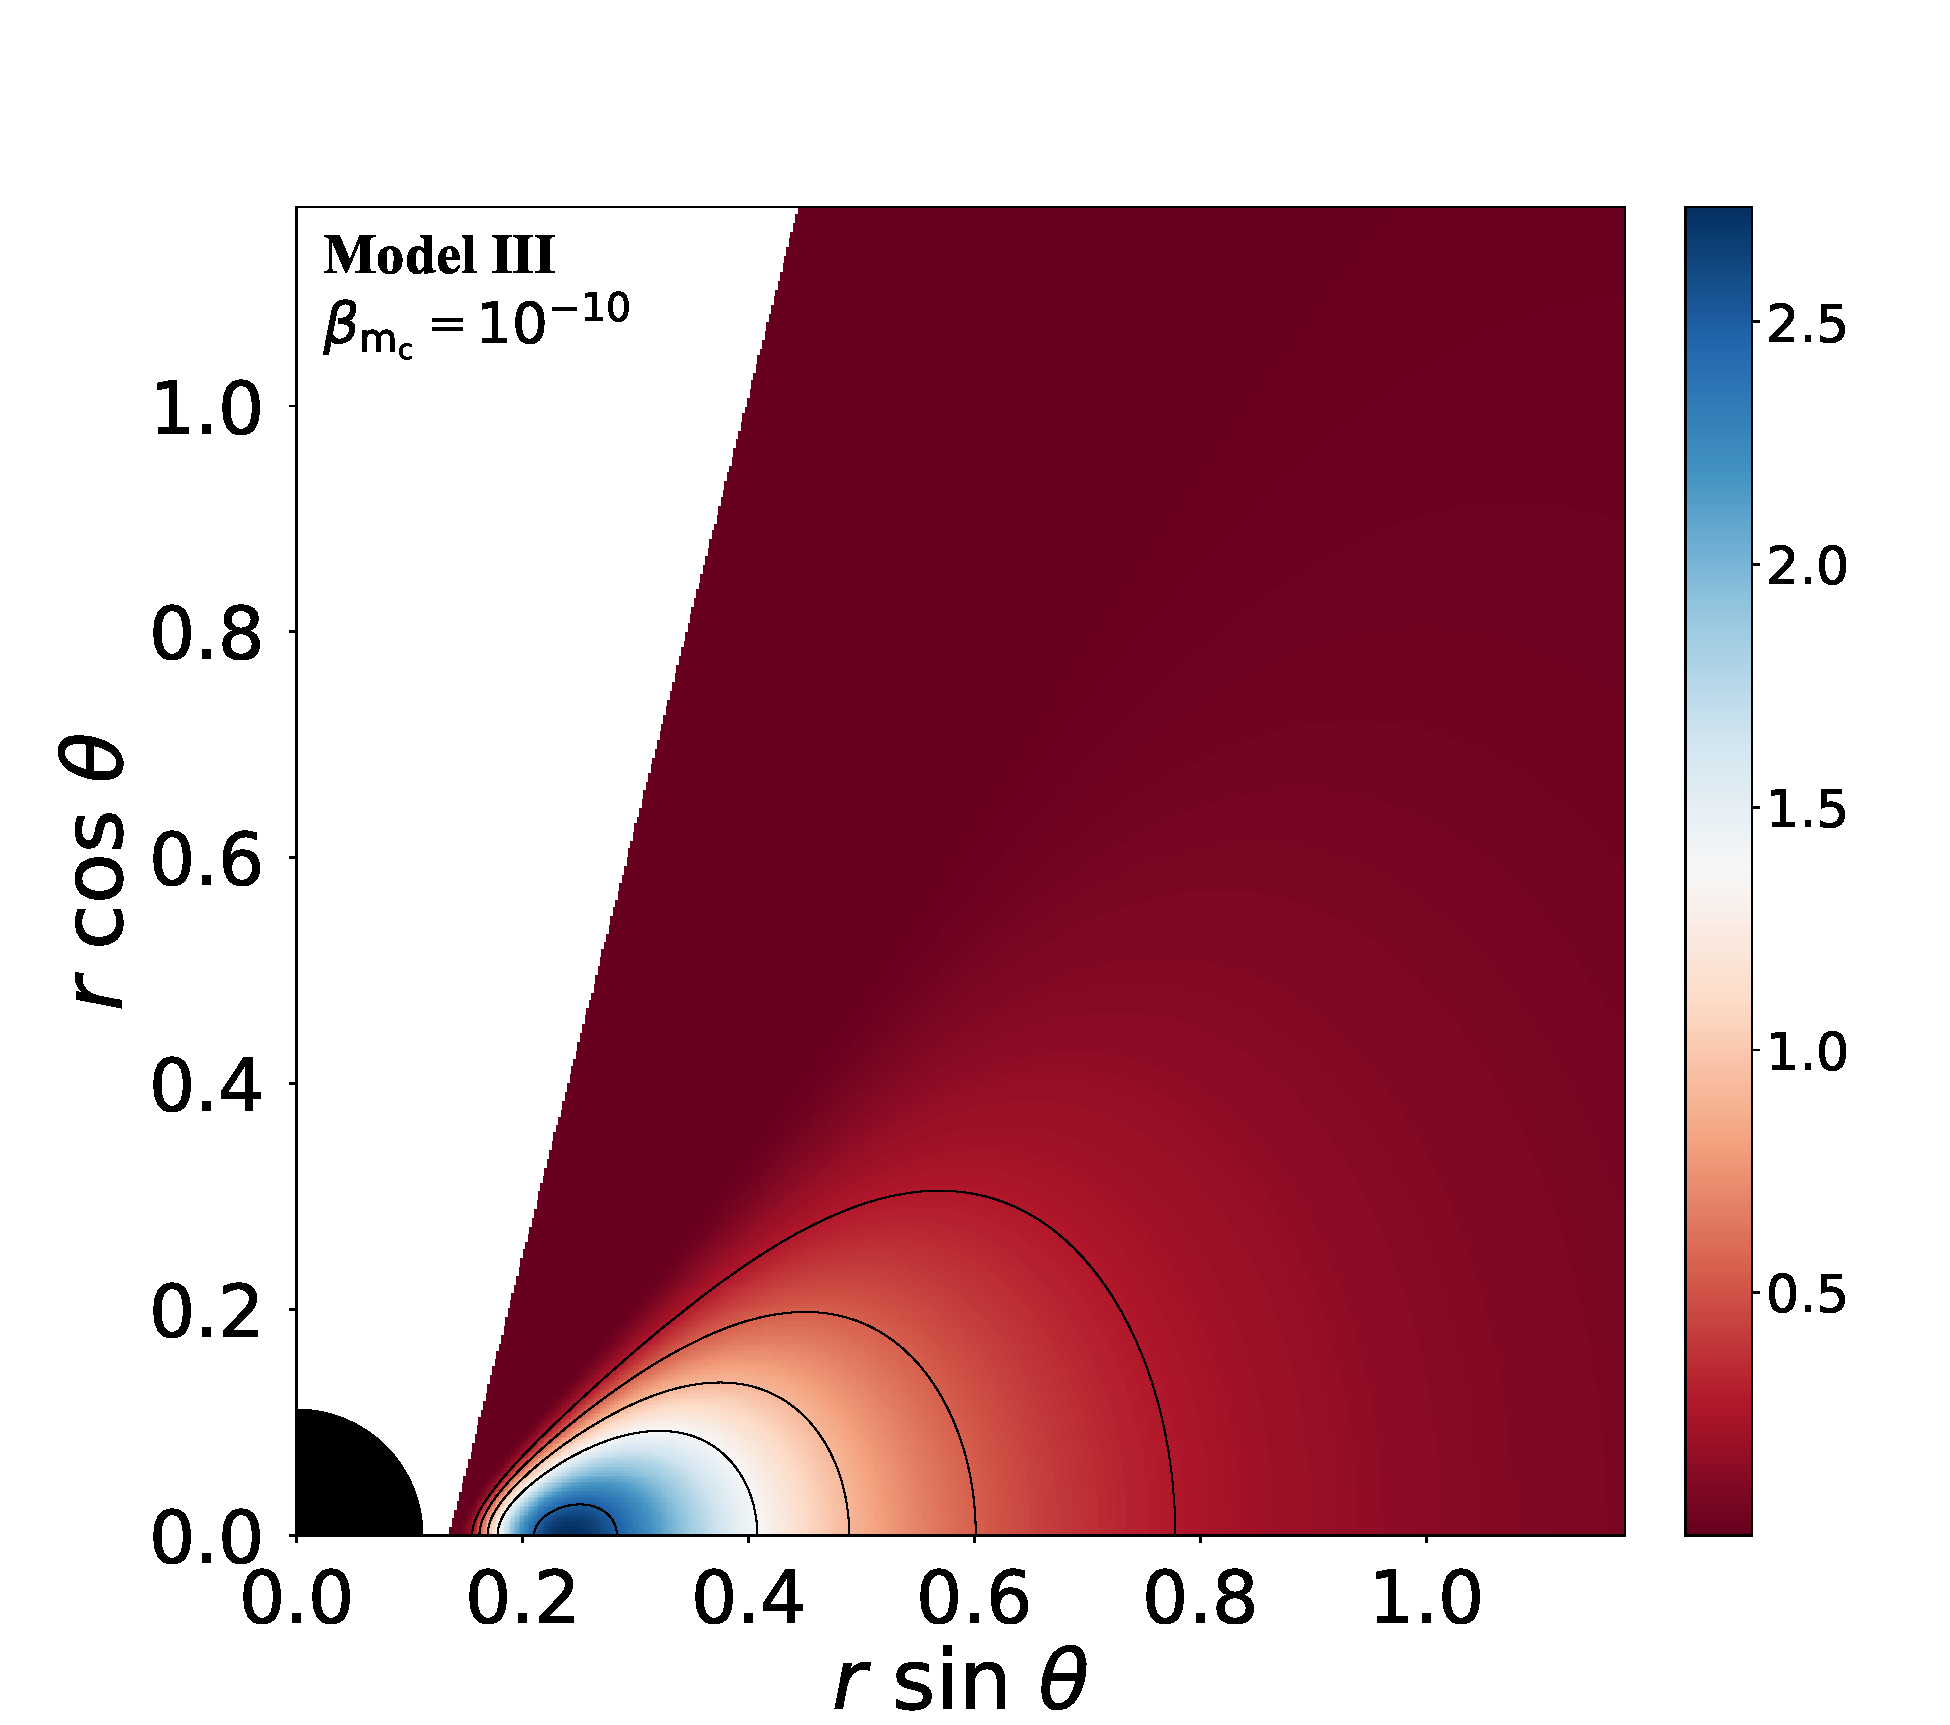
\includegraphics[scale=0.14]{figures/fig1_III__10.pdf}
\\
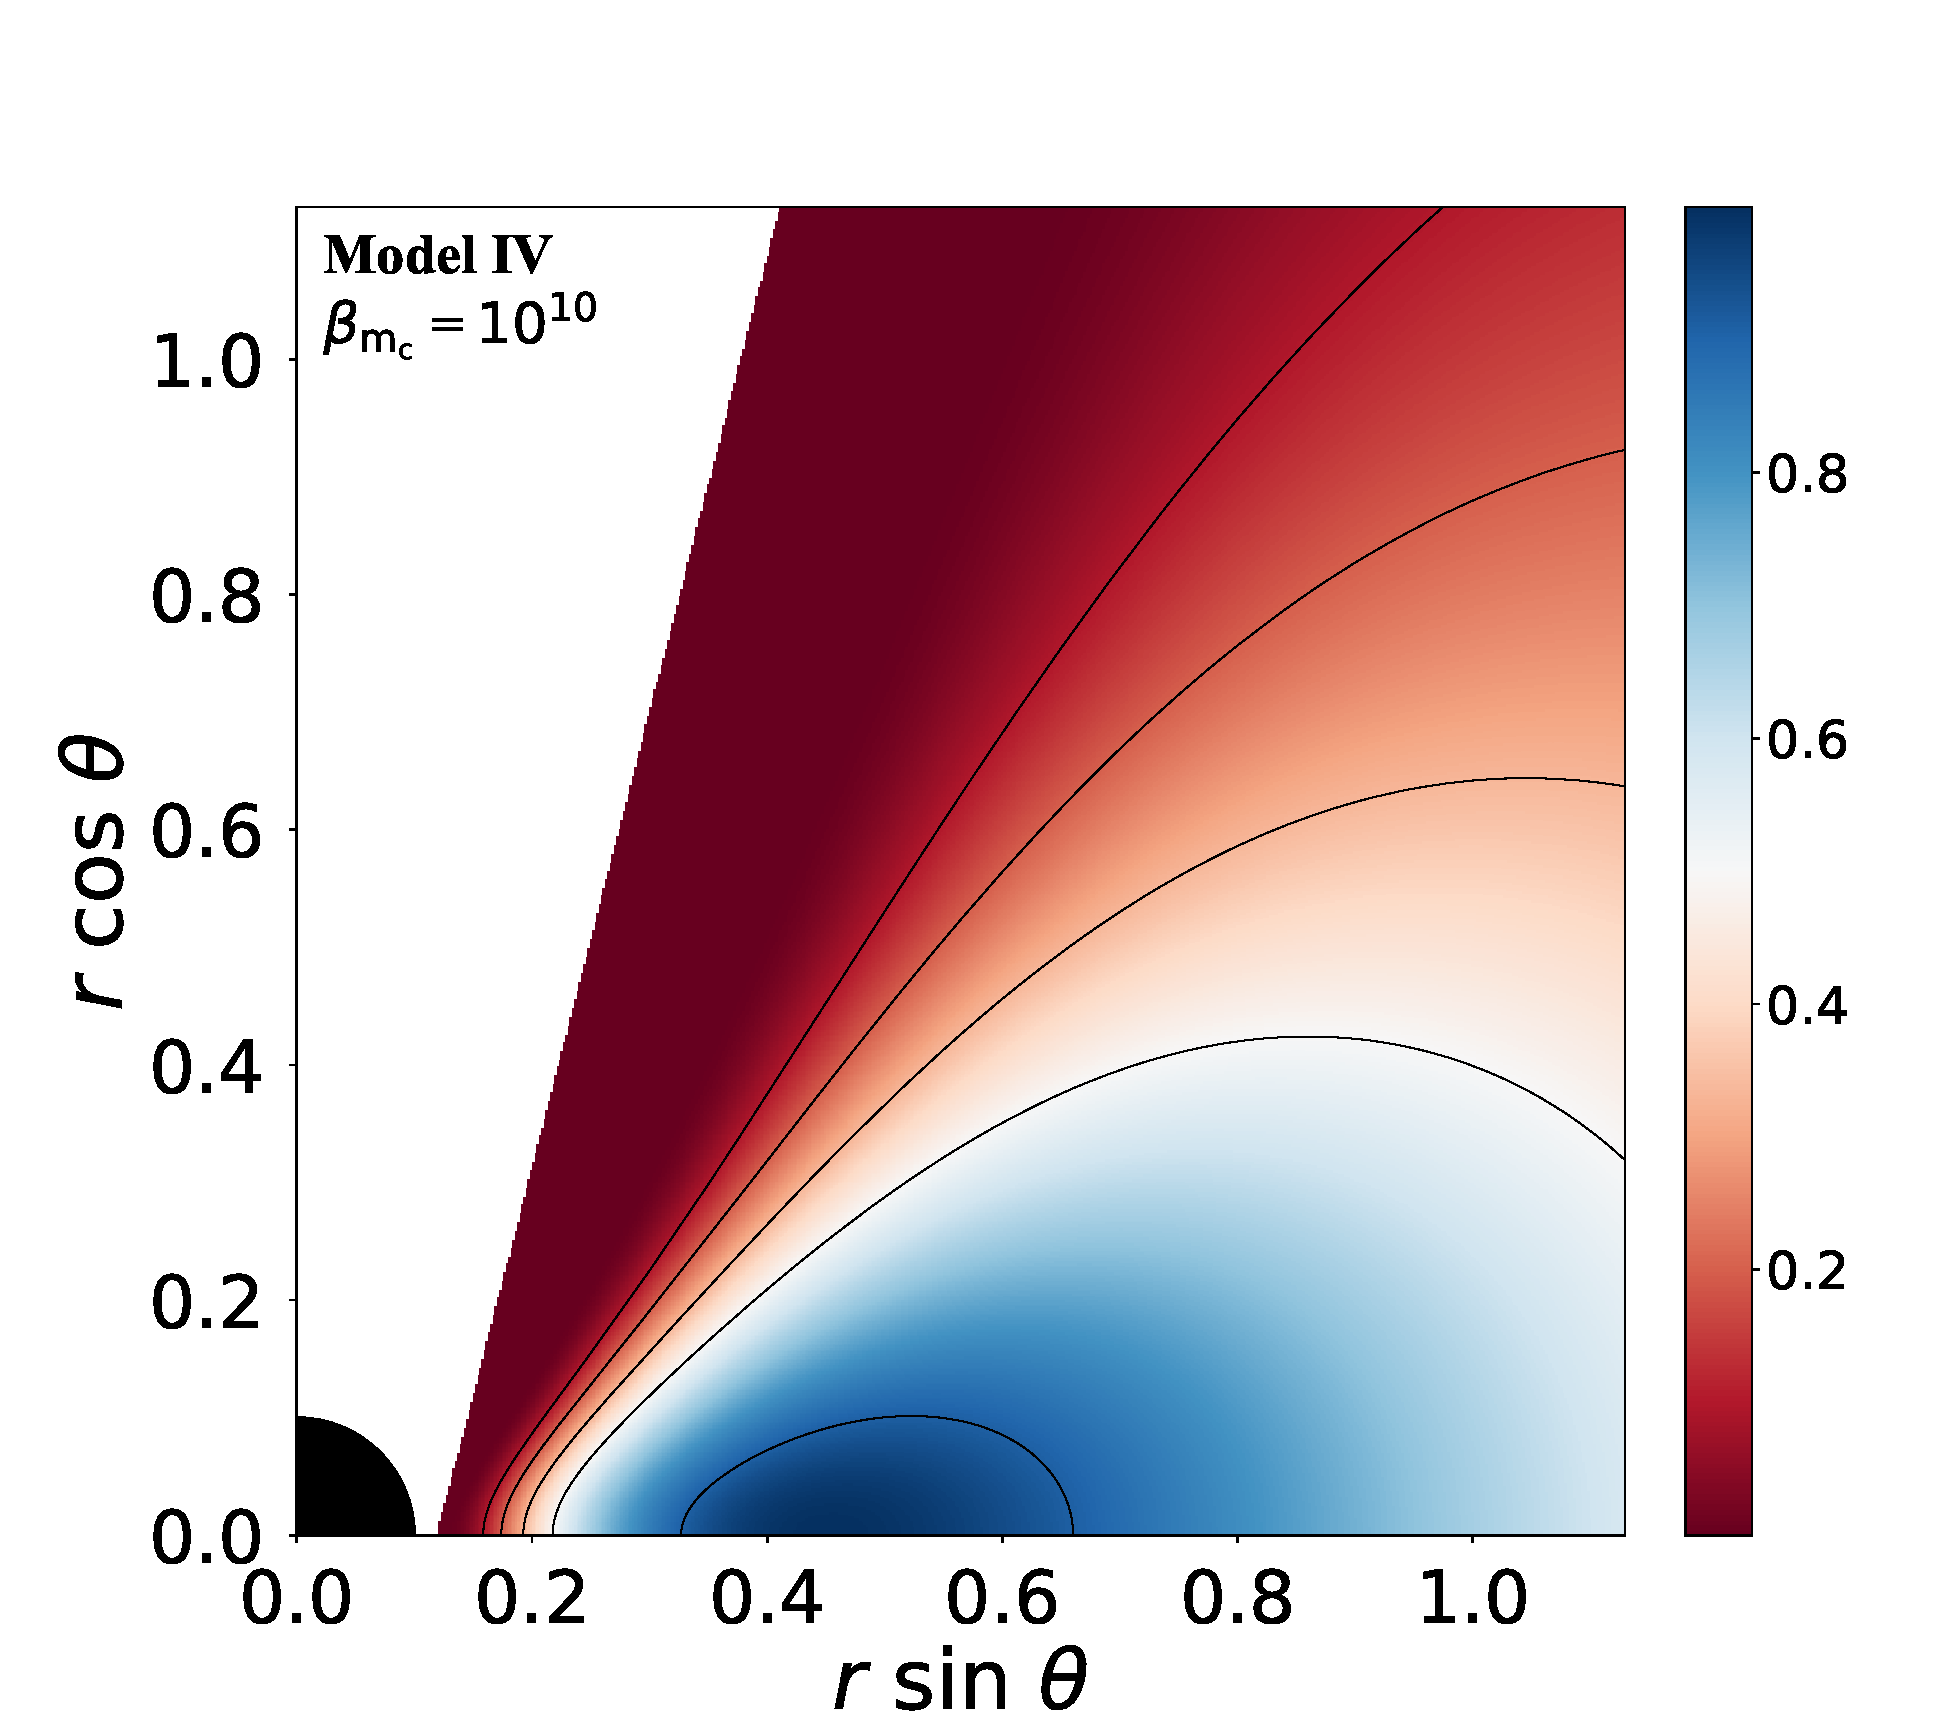
\includegraphics[scale=0.14]{figures/fig1_IV_10.pdf}
\hspace{-0.3cm}
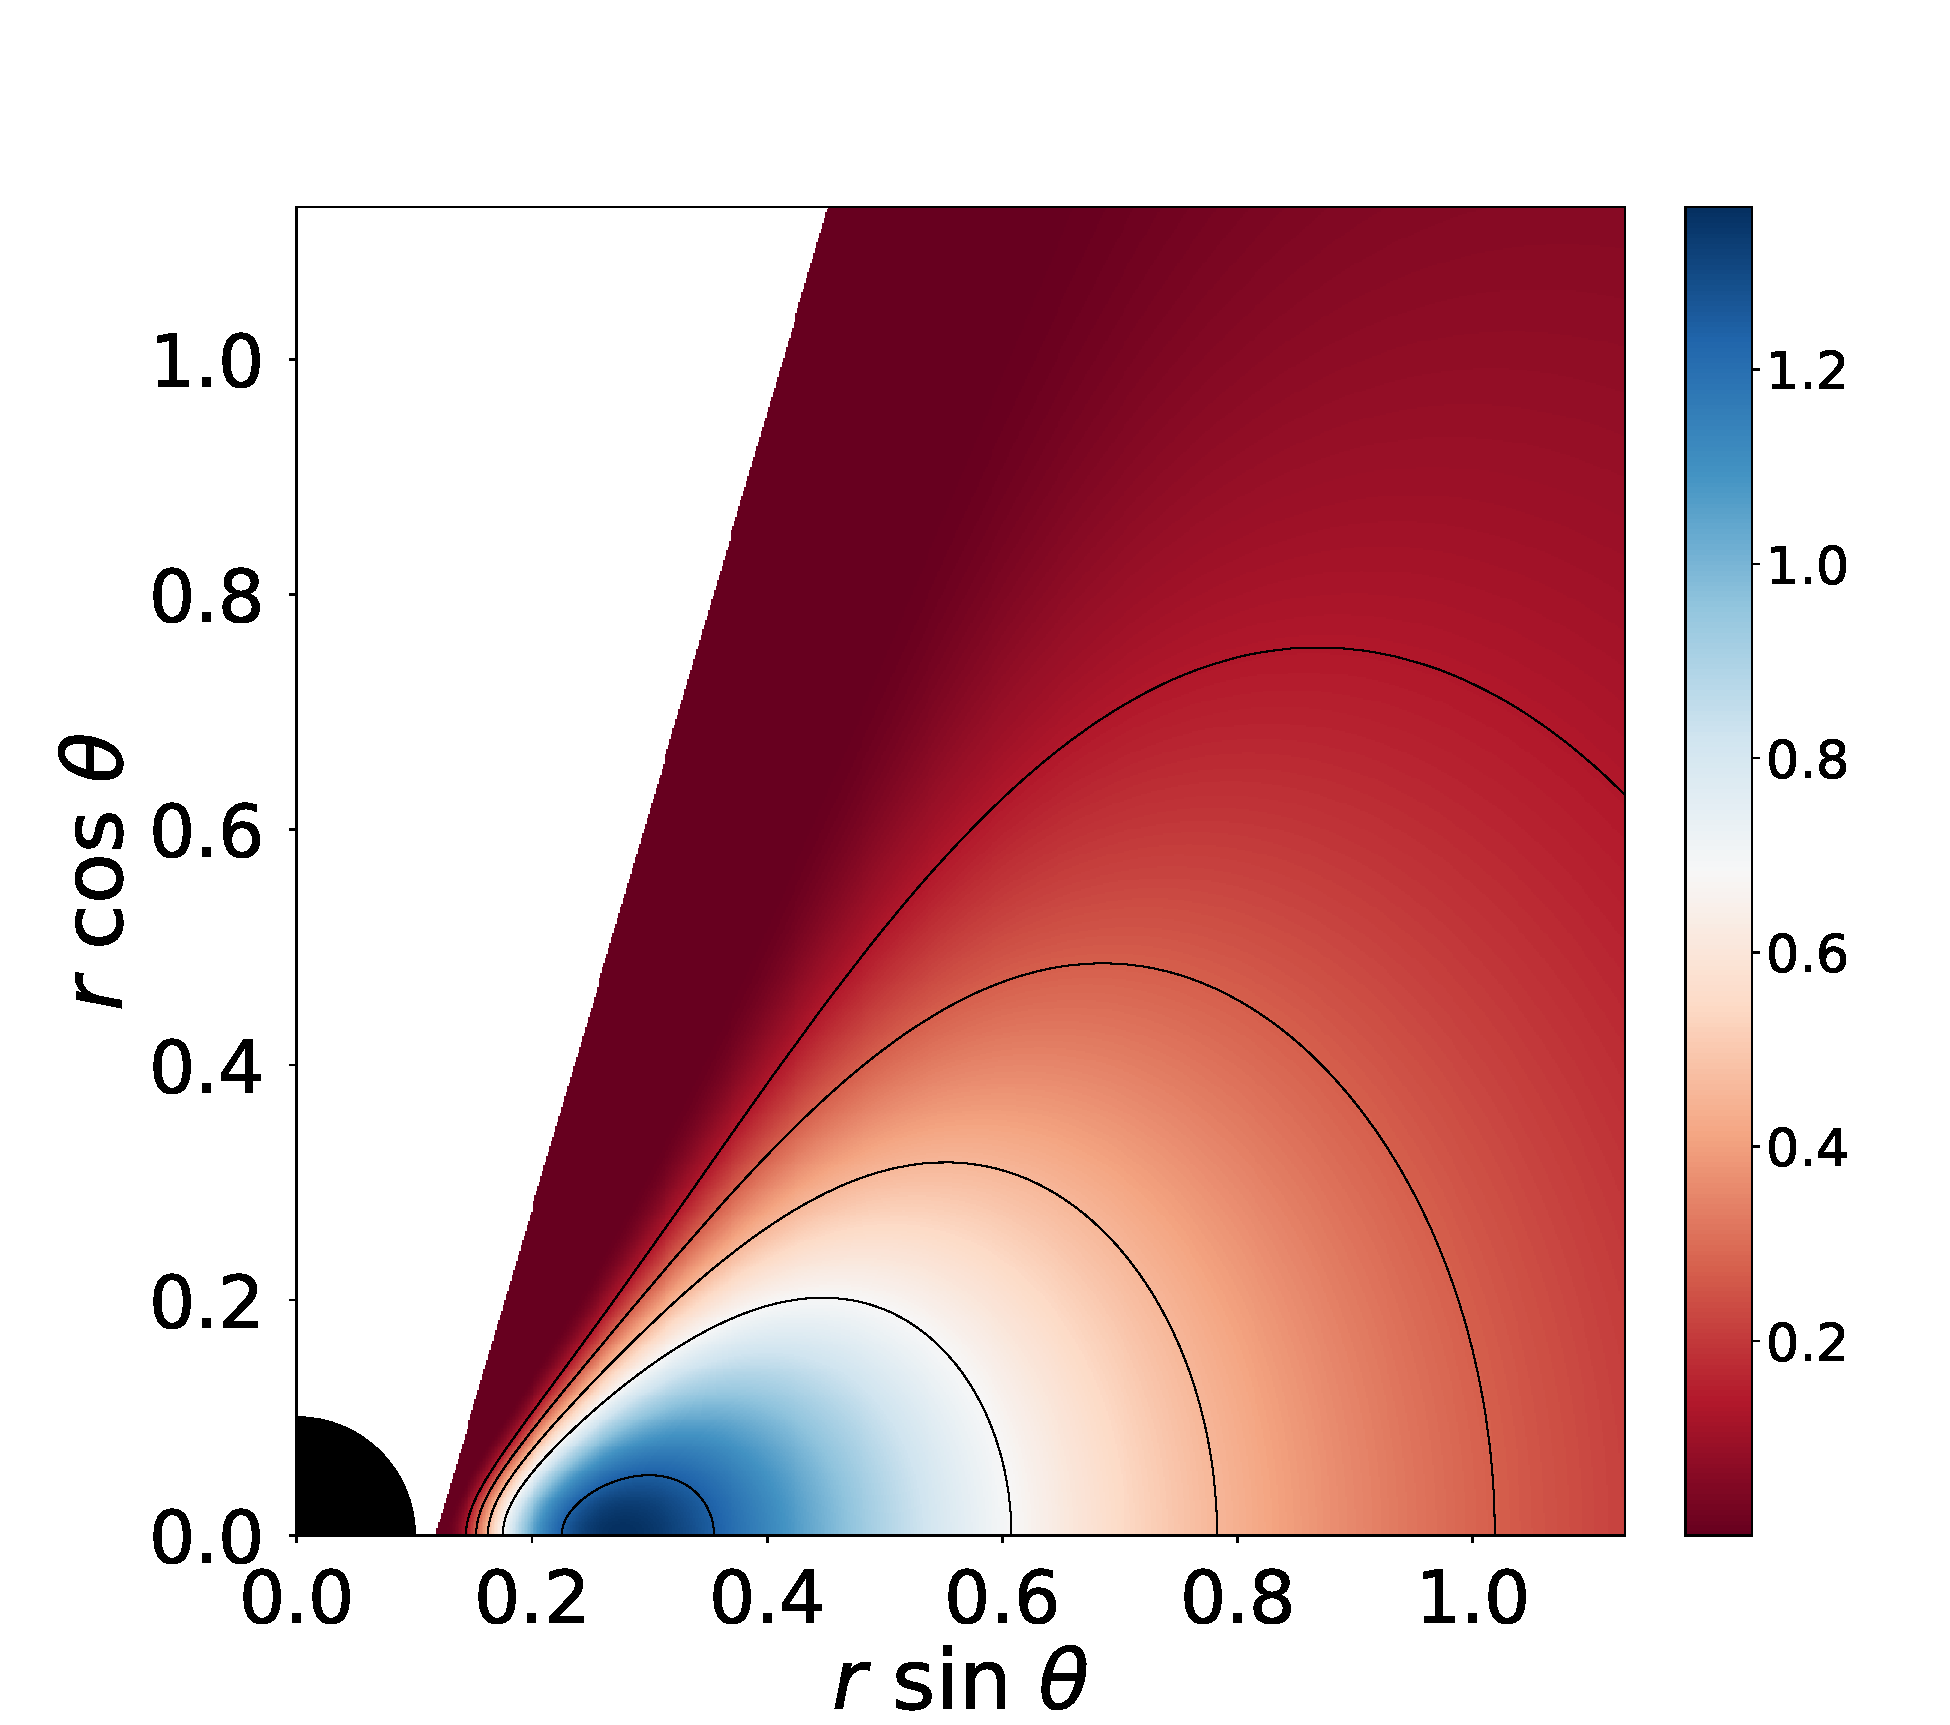
\includegraphics[scale=0.14]{figures/fig1_IV_1.pdf}
\hspace{-0.2cm}
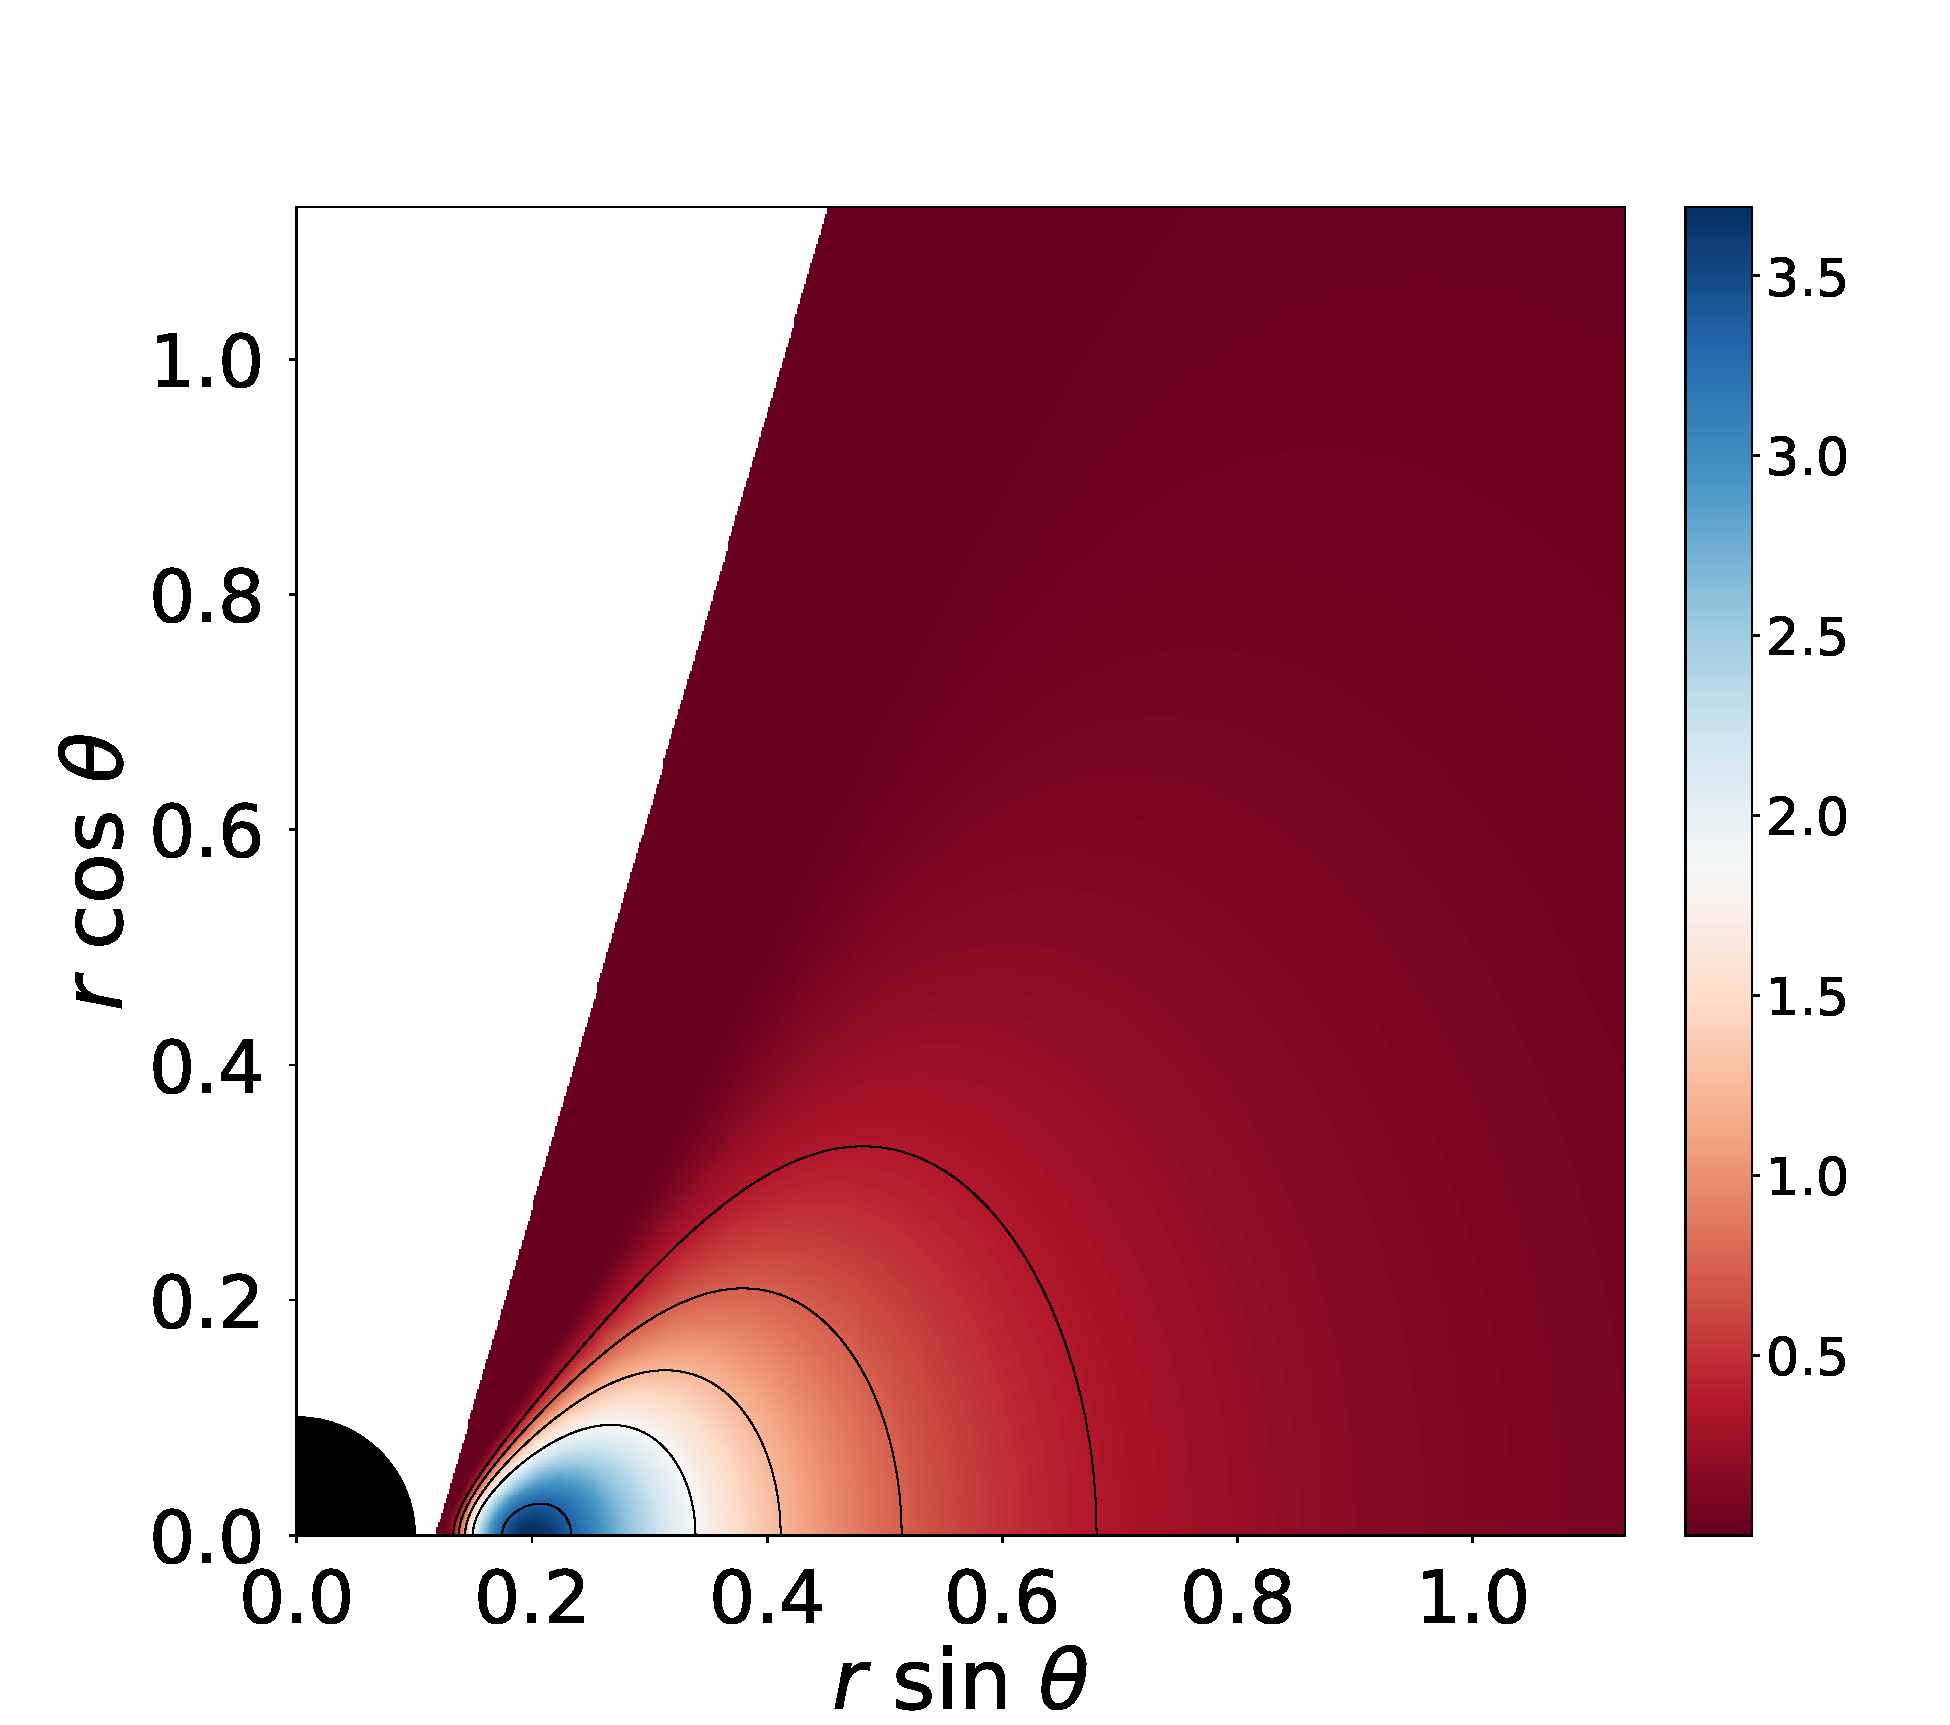
\includegraphics[scale=0.14]{figures/fig1_IV__10.pdf}
\hspace{-0.2cm}
\caption{Distribution of the logarithm of the rest-mass density. From top to bottom the rows correspond to the first four models of KBHsSH (I, II, III and IV). From left to right the columns correspond to different values of the magnetization parameter, namely non-magnetized ($\beta_{\mathrm{m}_{\mathrm{c}}} = 10^{10}$), mildly magnetized ($\beta_{\mathrm{m}_{\mathrm{c}}} = 1$) and strongly magnetized ($\beta_{\mathrm{m}_{\mathrm{c}}} = 10^{-10}$). The range of the colour scale is not the same for all plots.
\tf{Perhaps it would be good to include in the upper left corner of each plot a legend indicating the model (e.g. Model I) and the value of $\beta_{\mathrm{m}_{\mathrm{c}}}$.}
}
\label{models_I}
\end{figure*}

\begin{figure*}
\centering
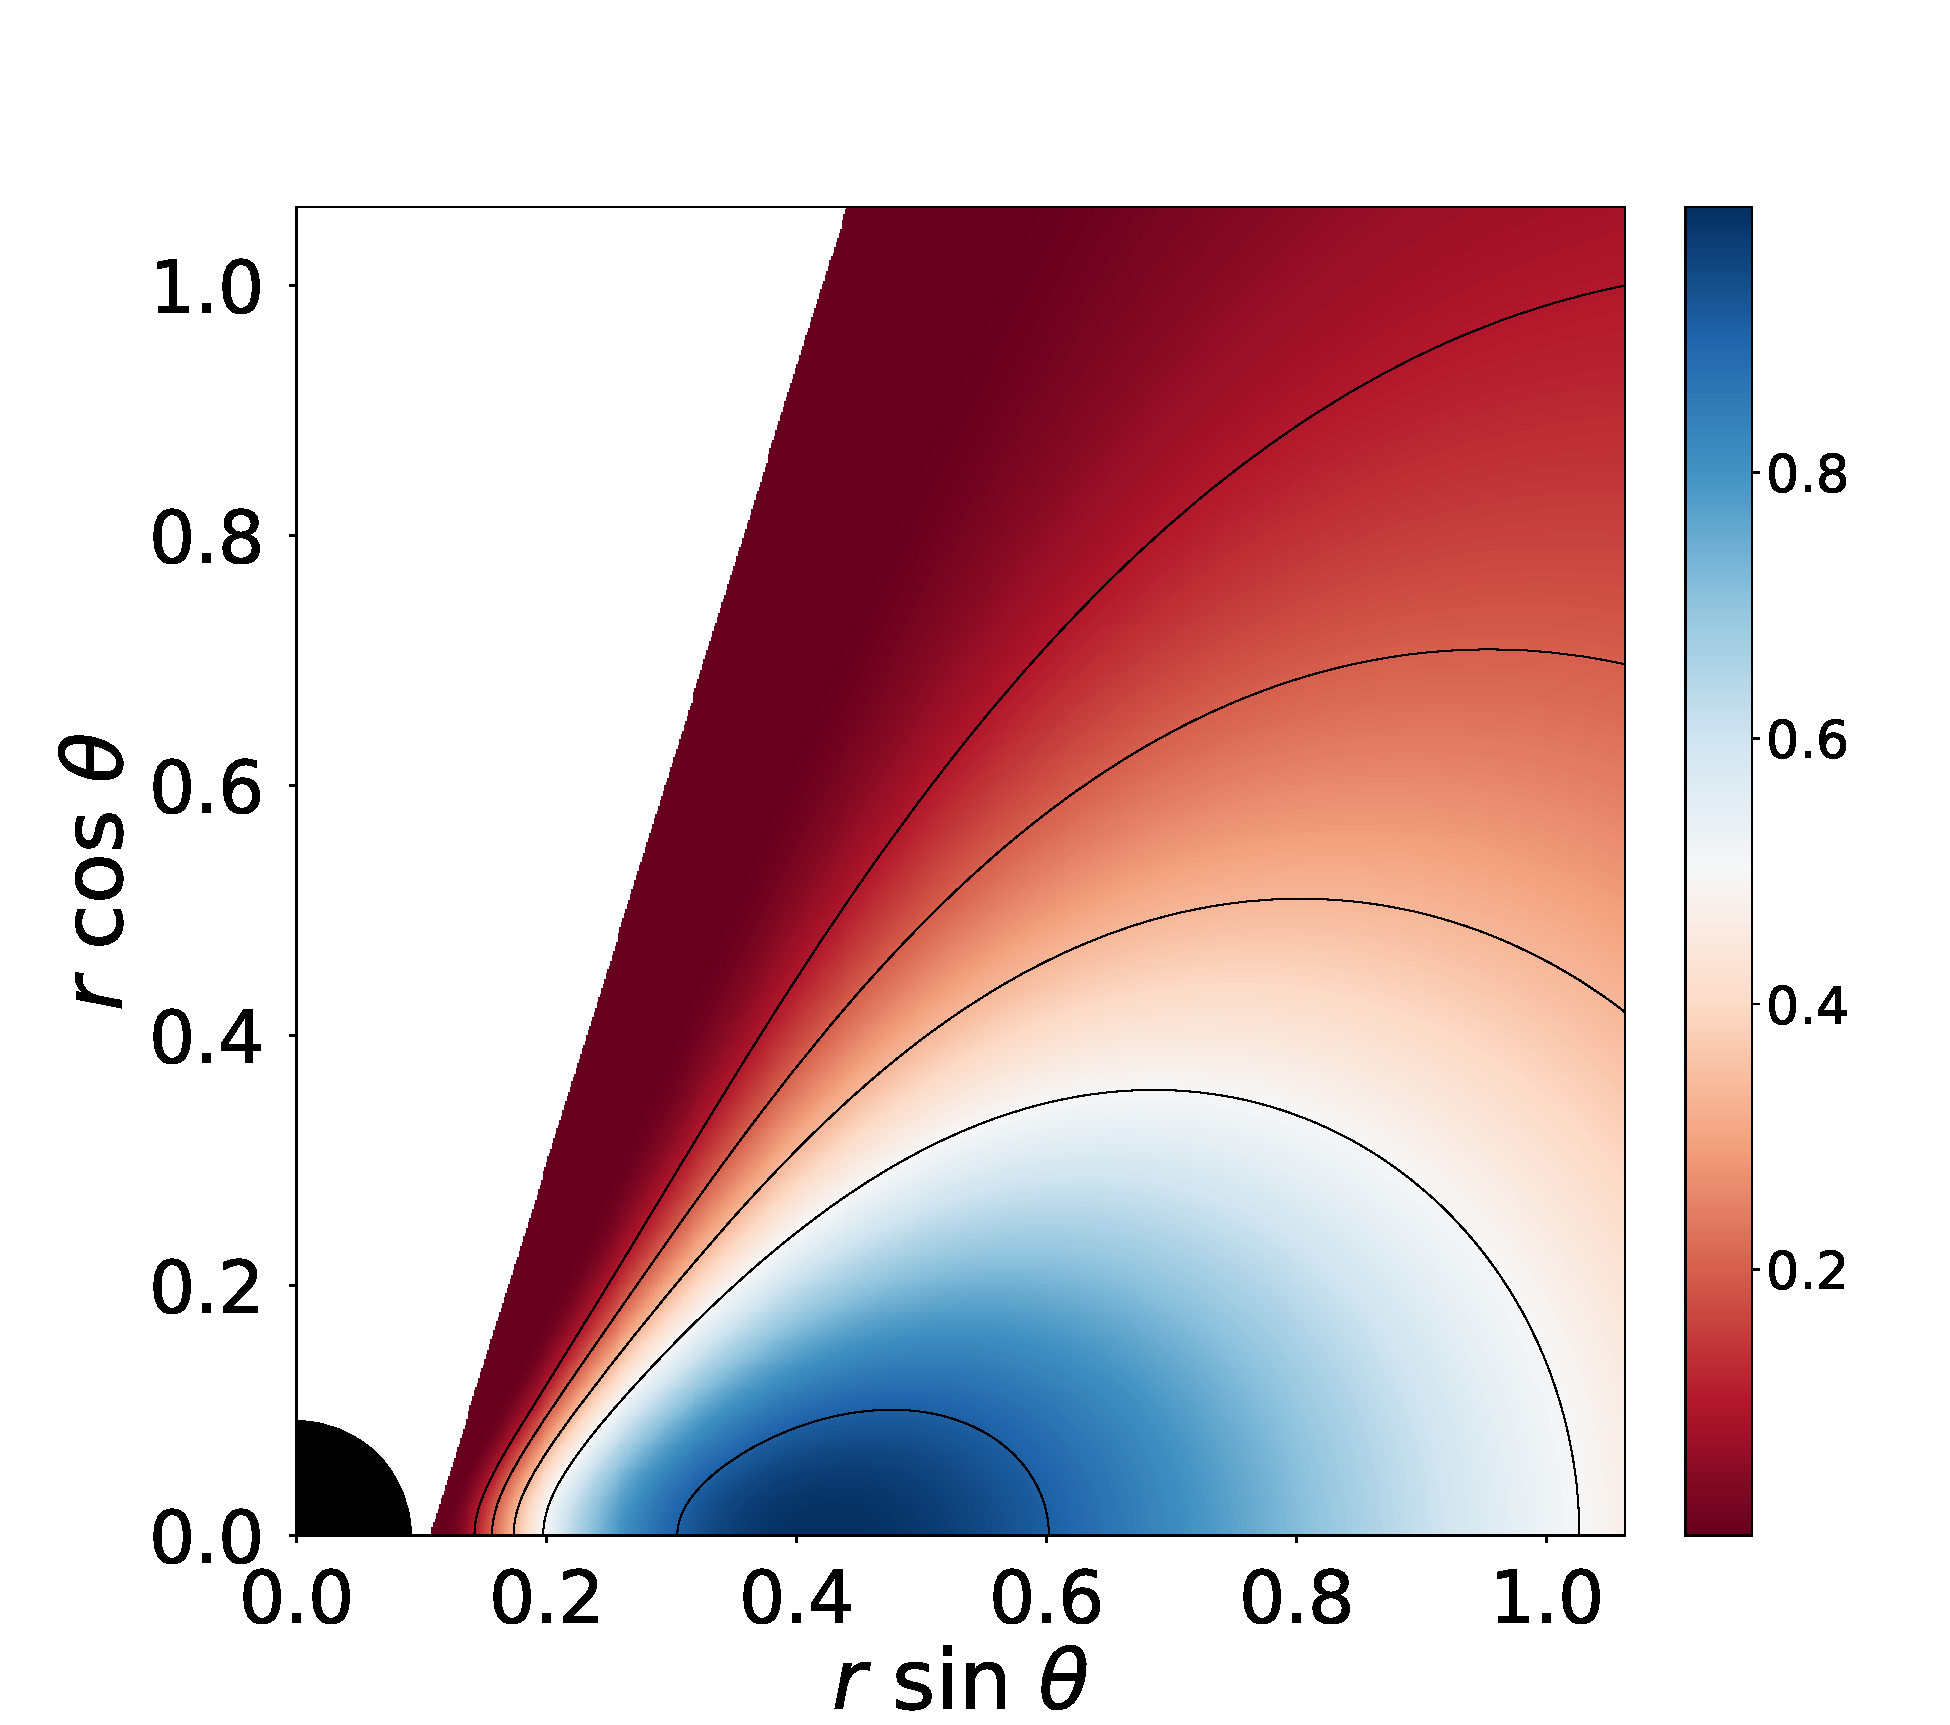
\includegraphics[scale=0.14]{figures/fig2_V_10.pdf}
\hspace{-0.3cm}
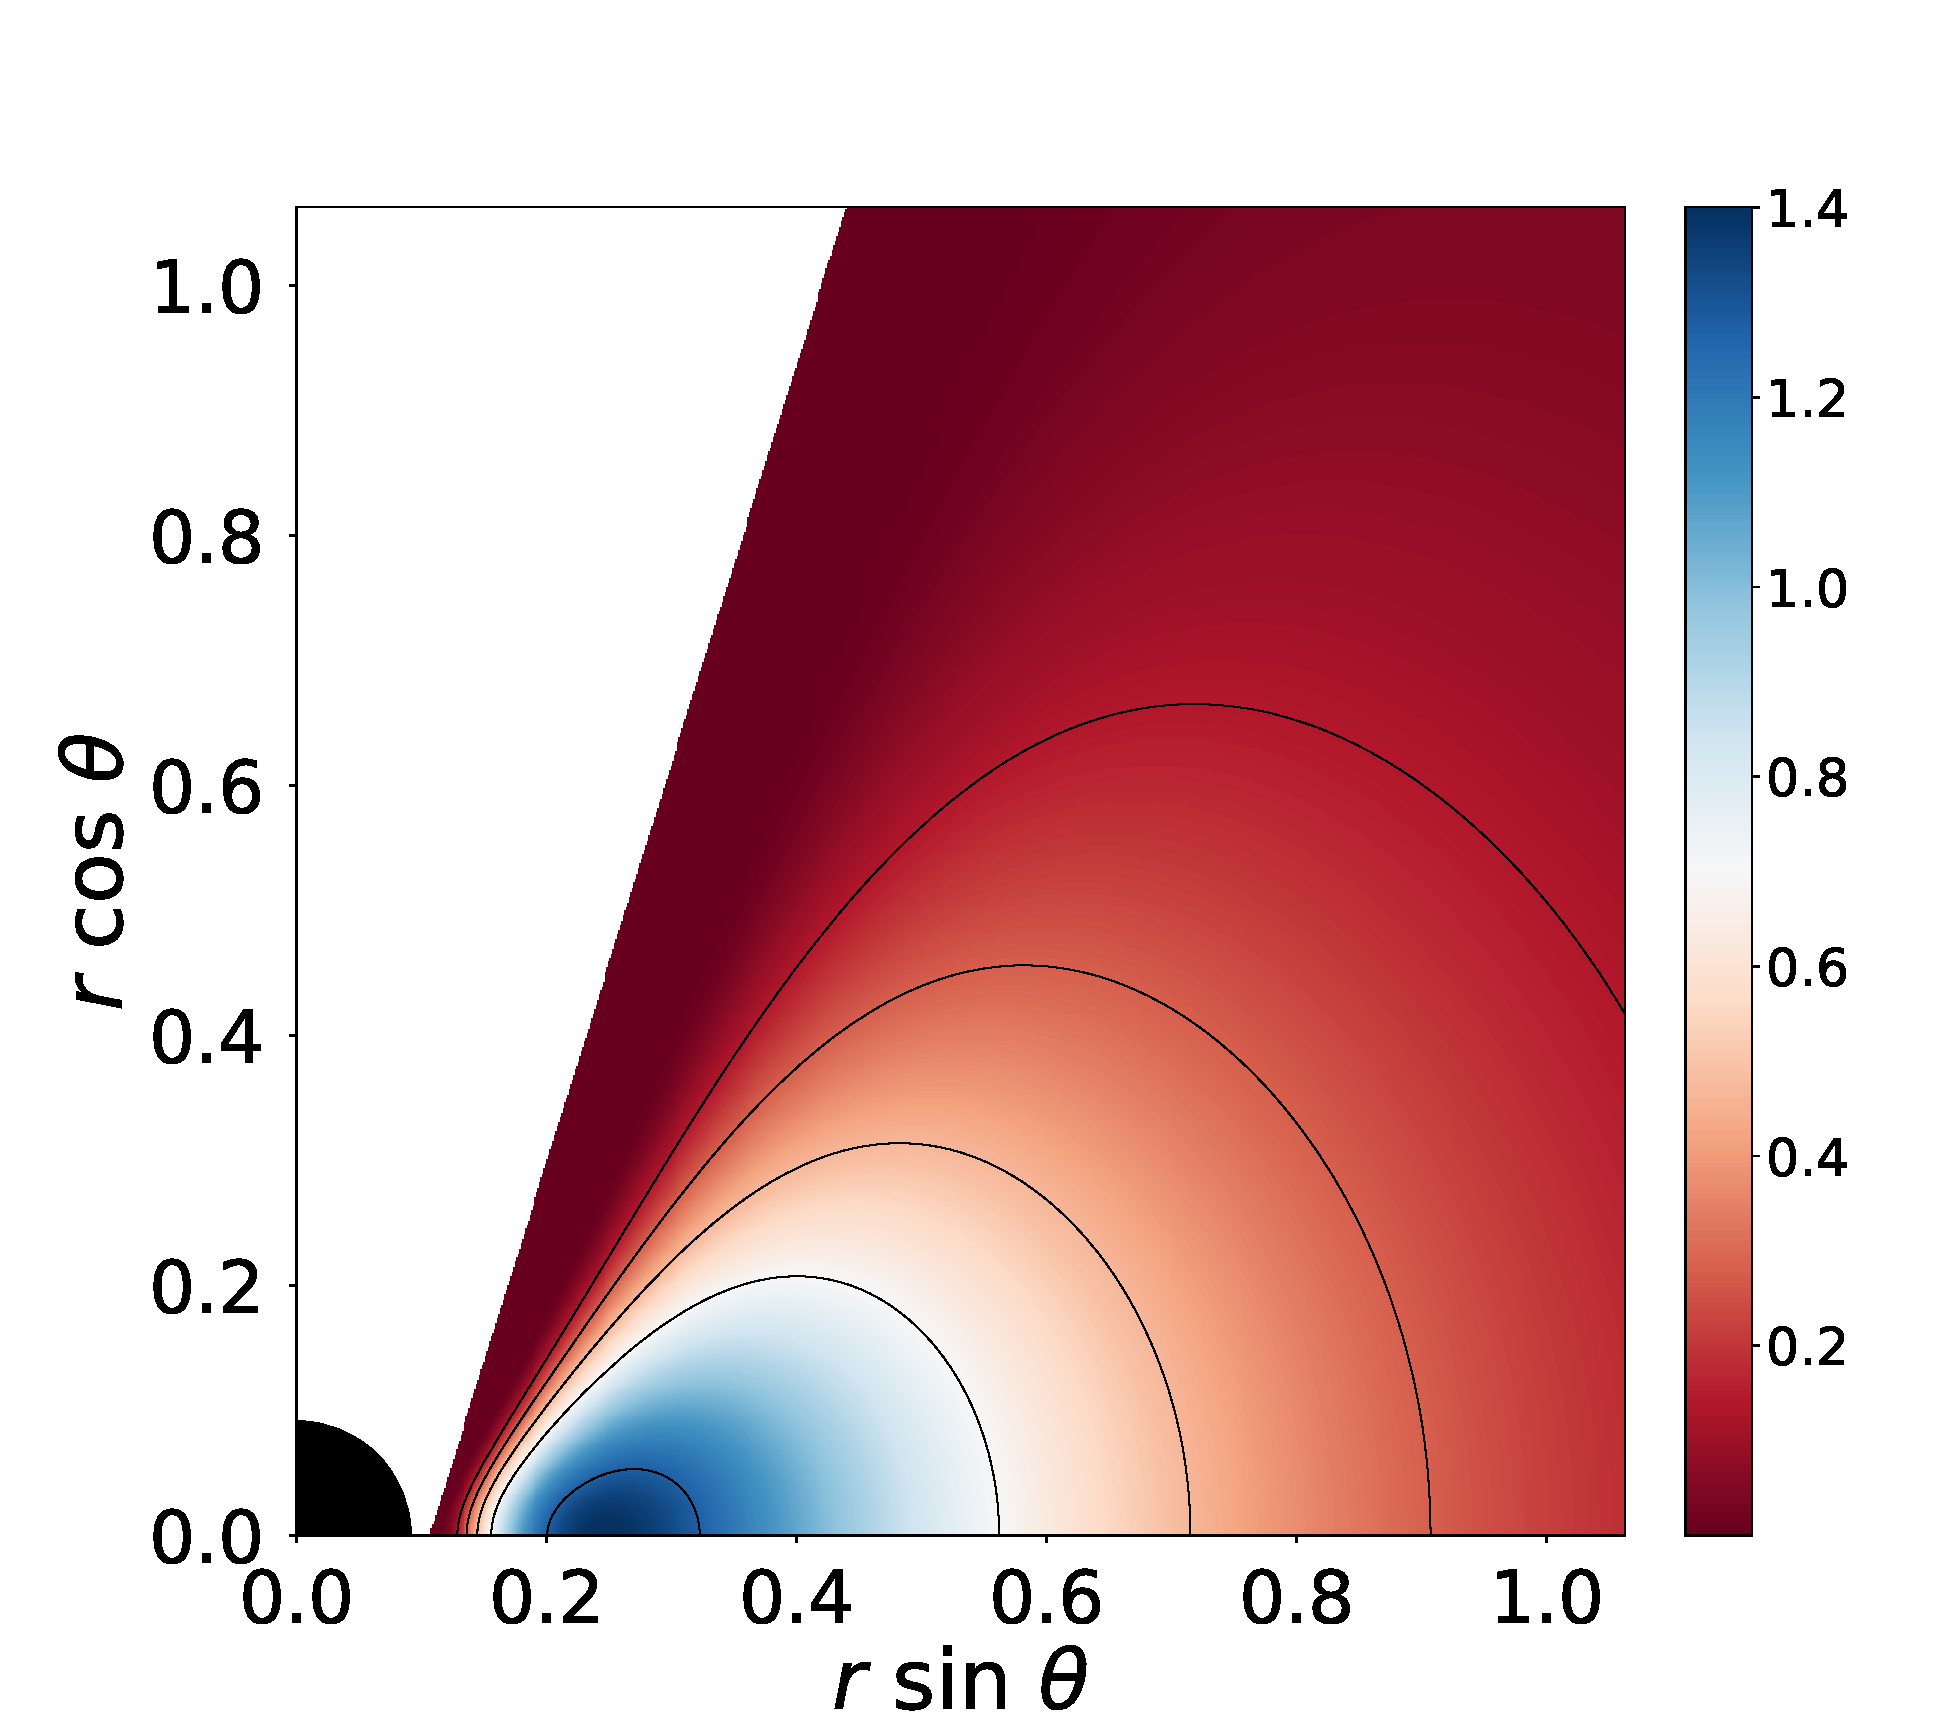
\includegraphics[scale=0.14]{figures/fig2_V_1.pdf}
\hspace{-0.2cm}
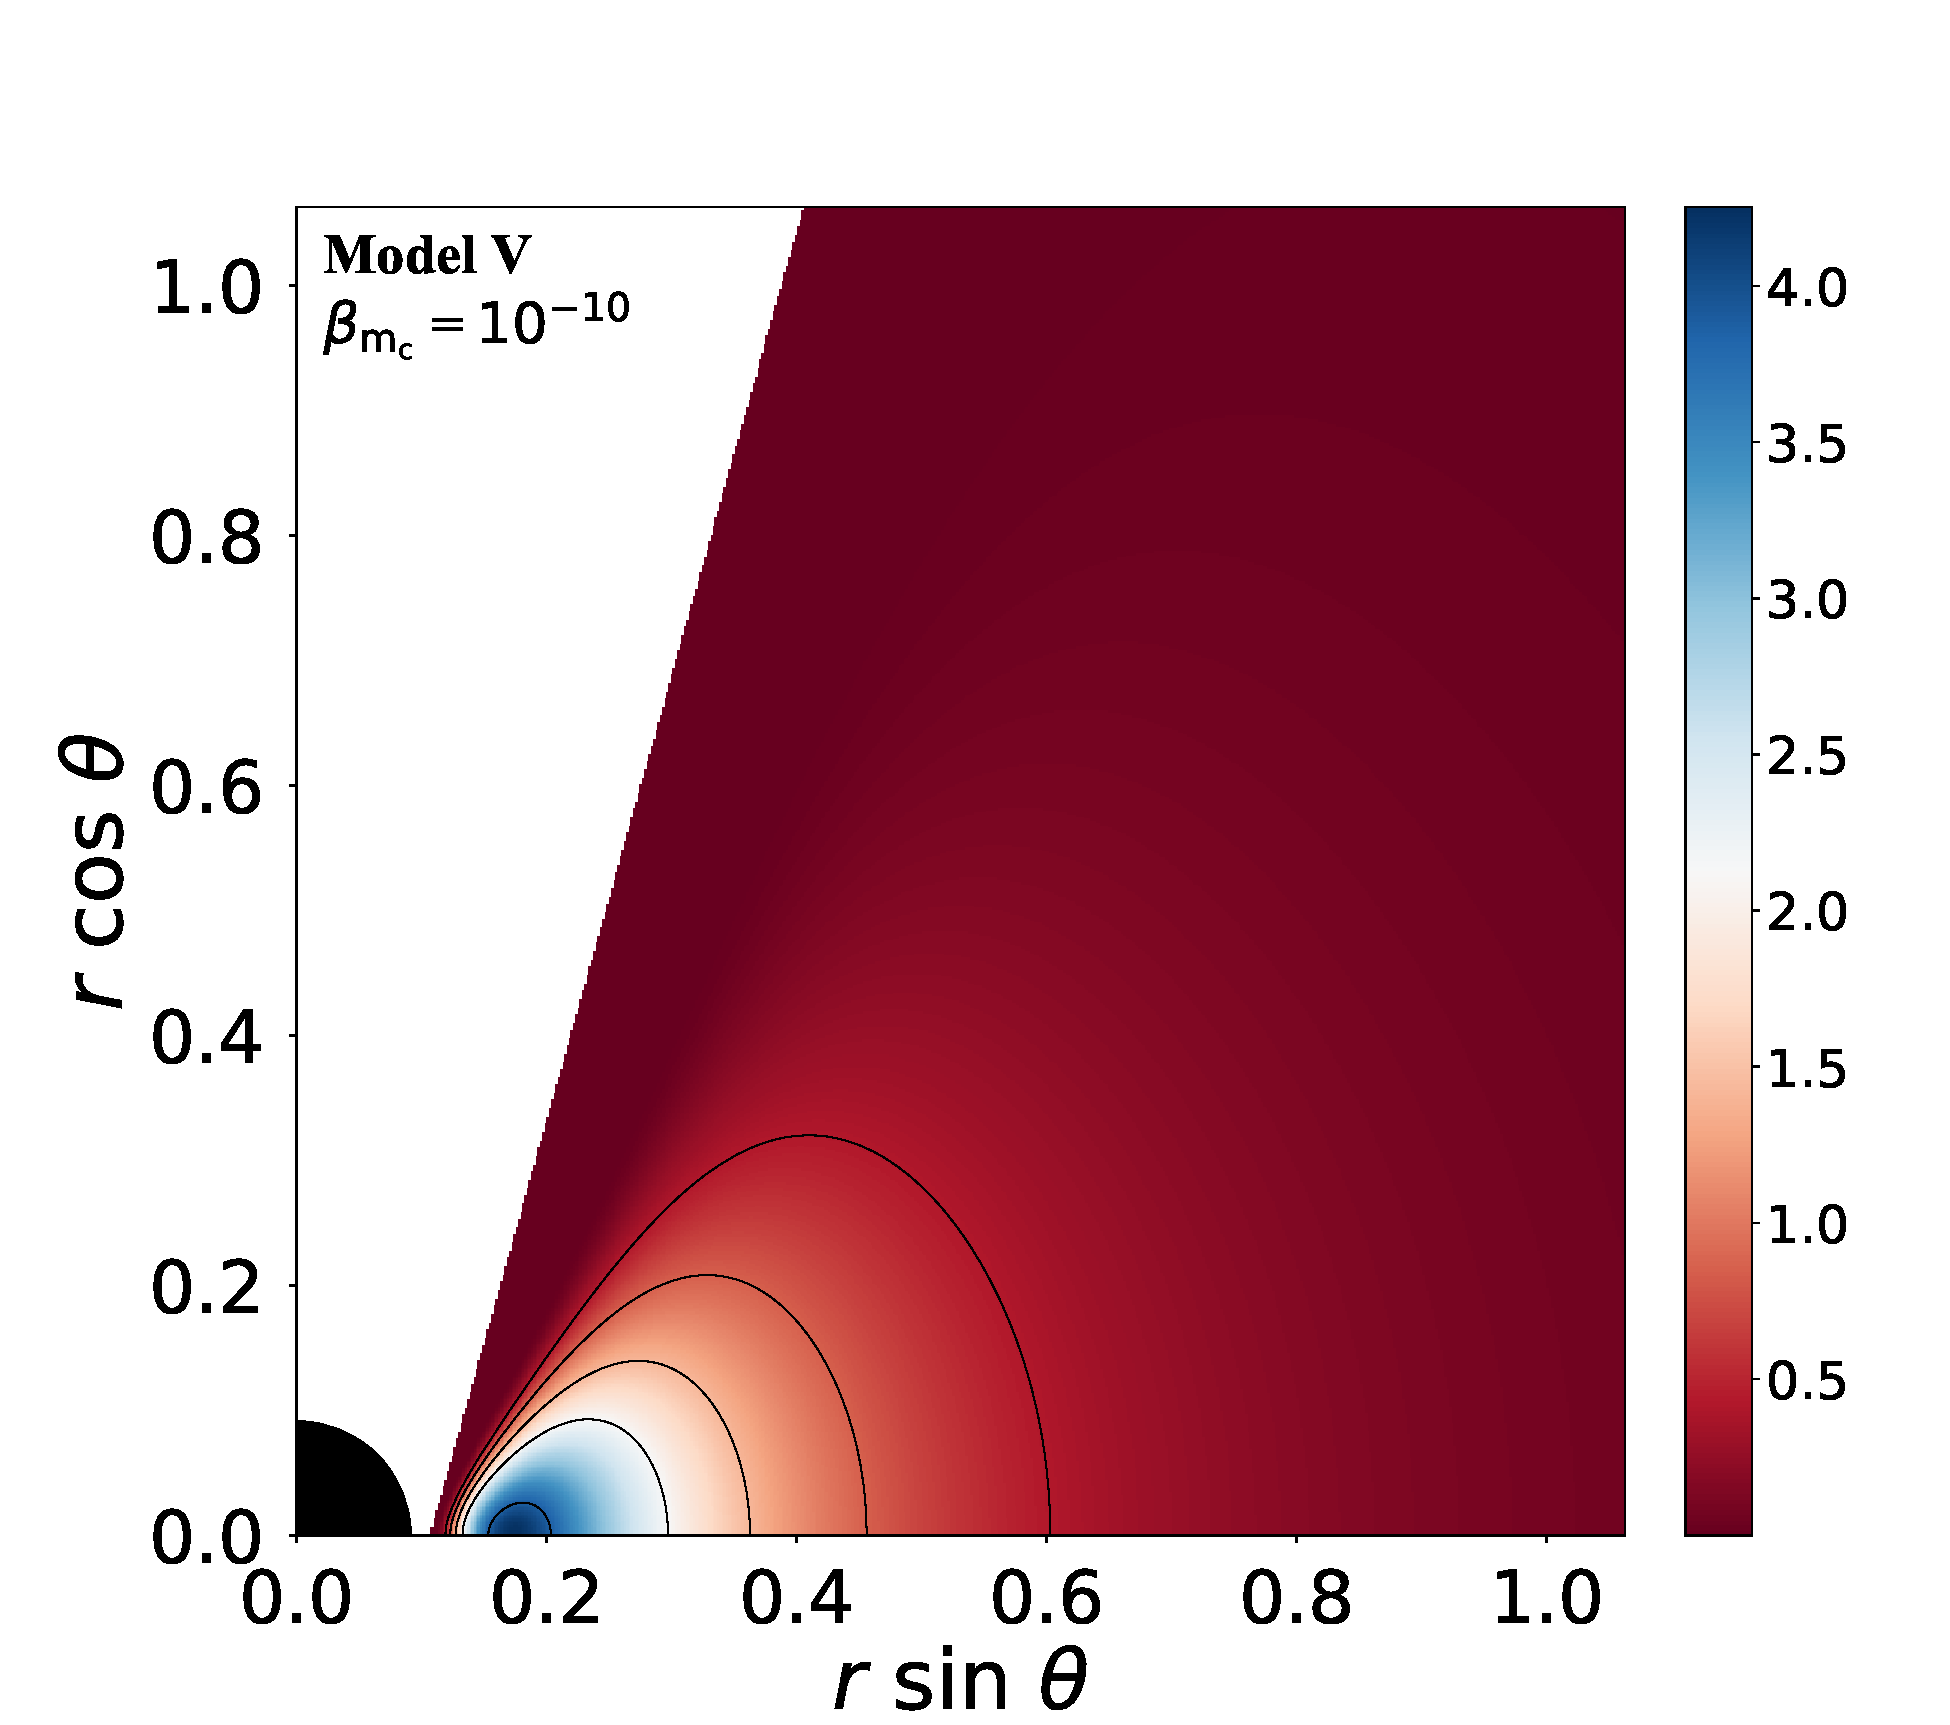
\includegraphics[scale=0.14]{figures/fig2_V__10.pdf}
\\
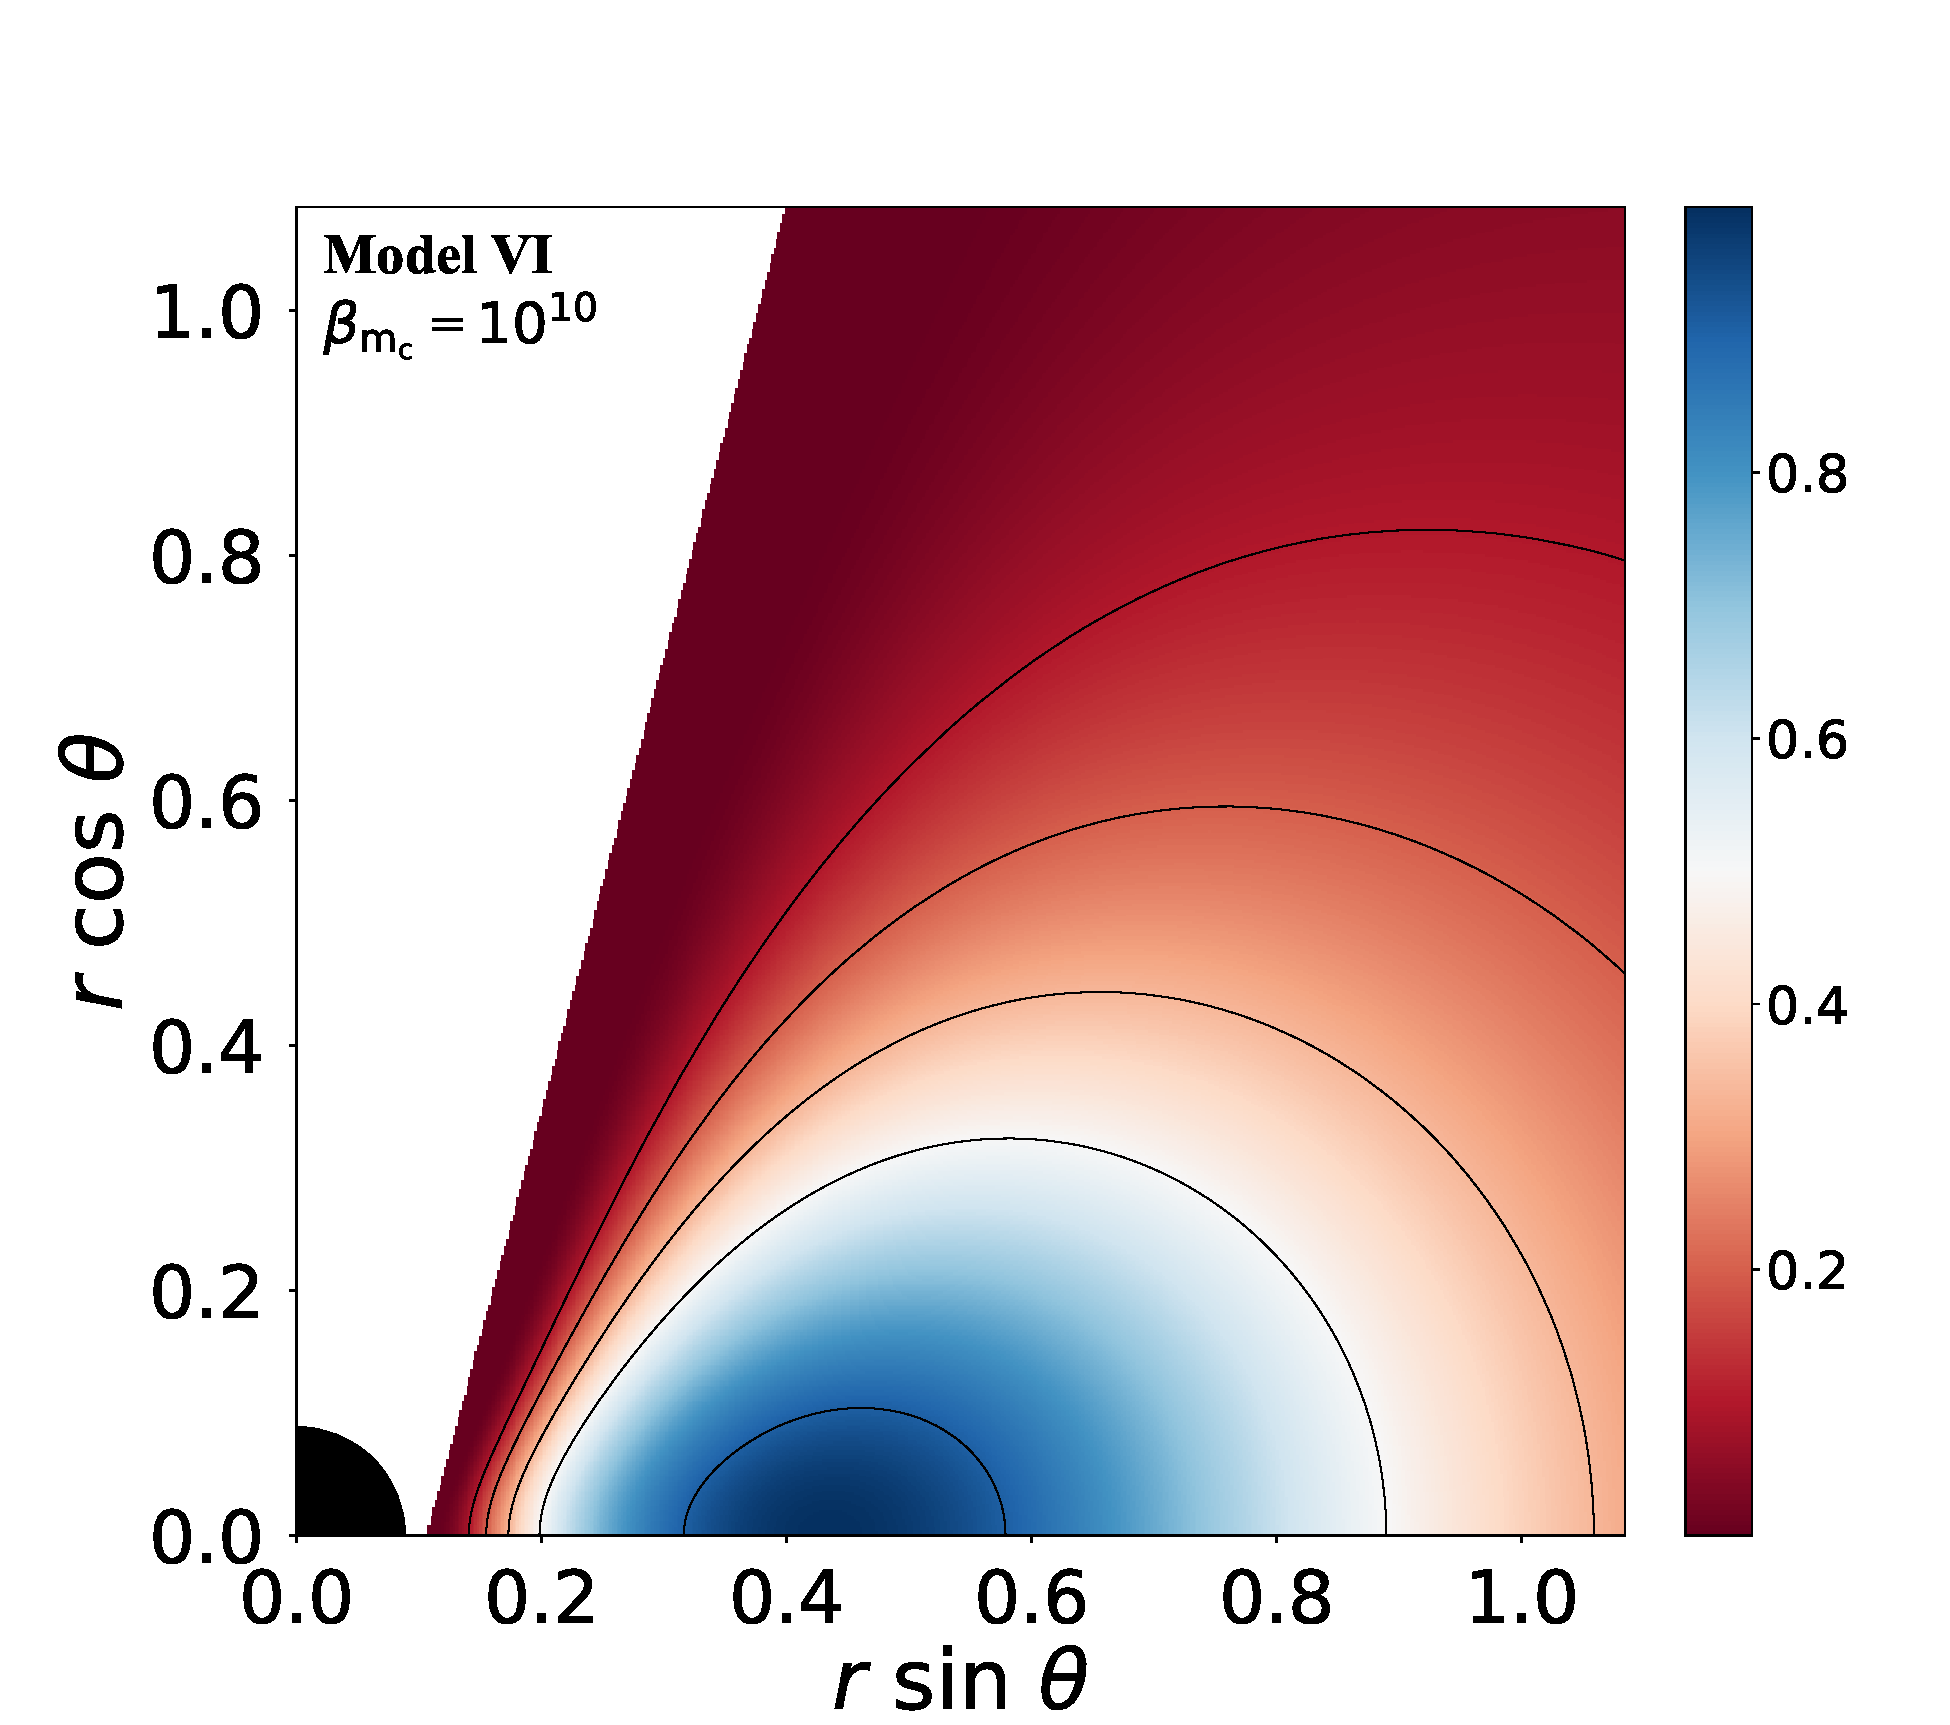
\includegraphics[scale=0.14]{figures/fig2_VI_10.pdf}
\hspace{-0.3cm}
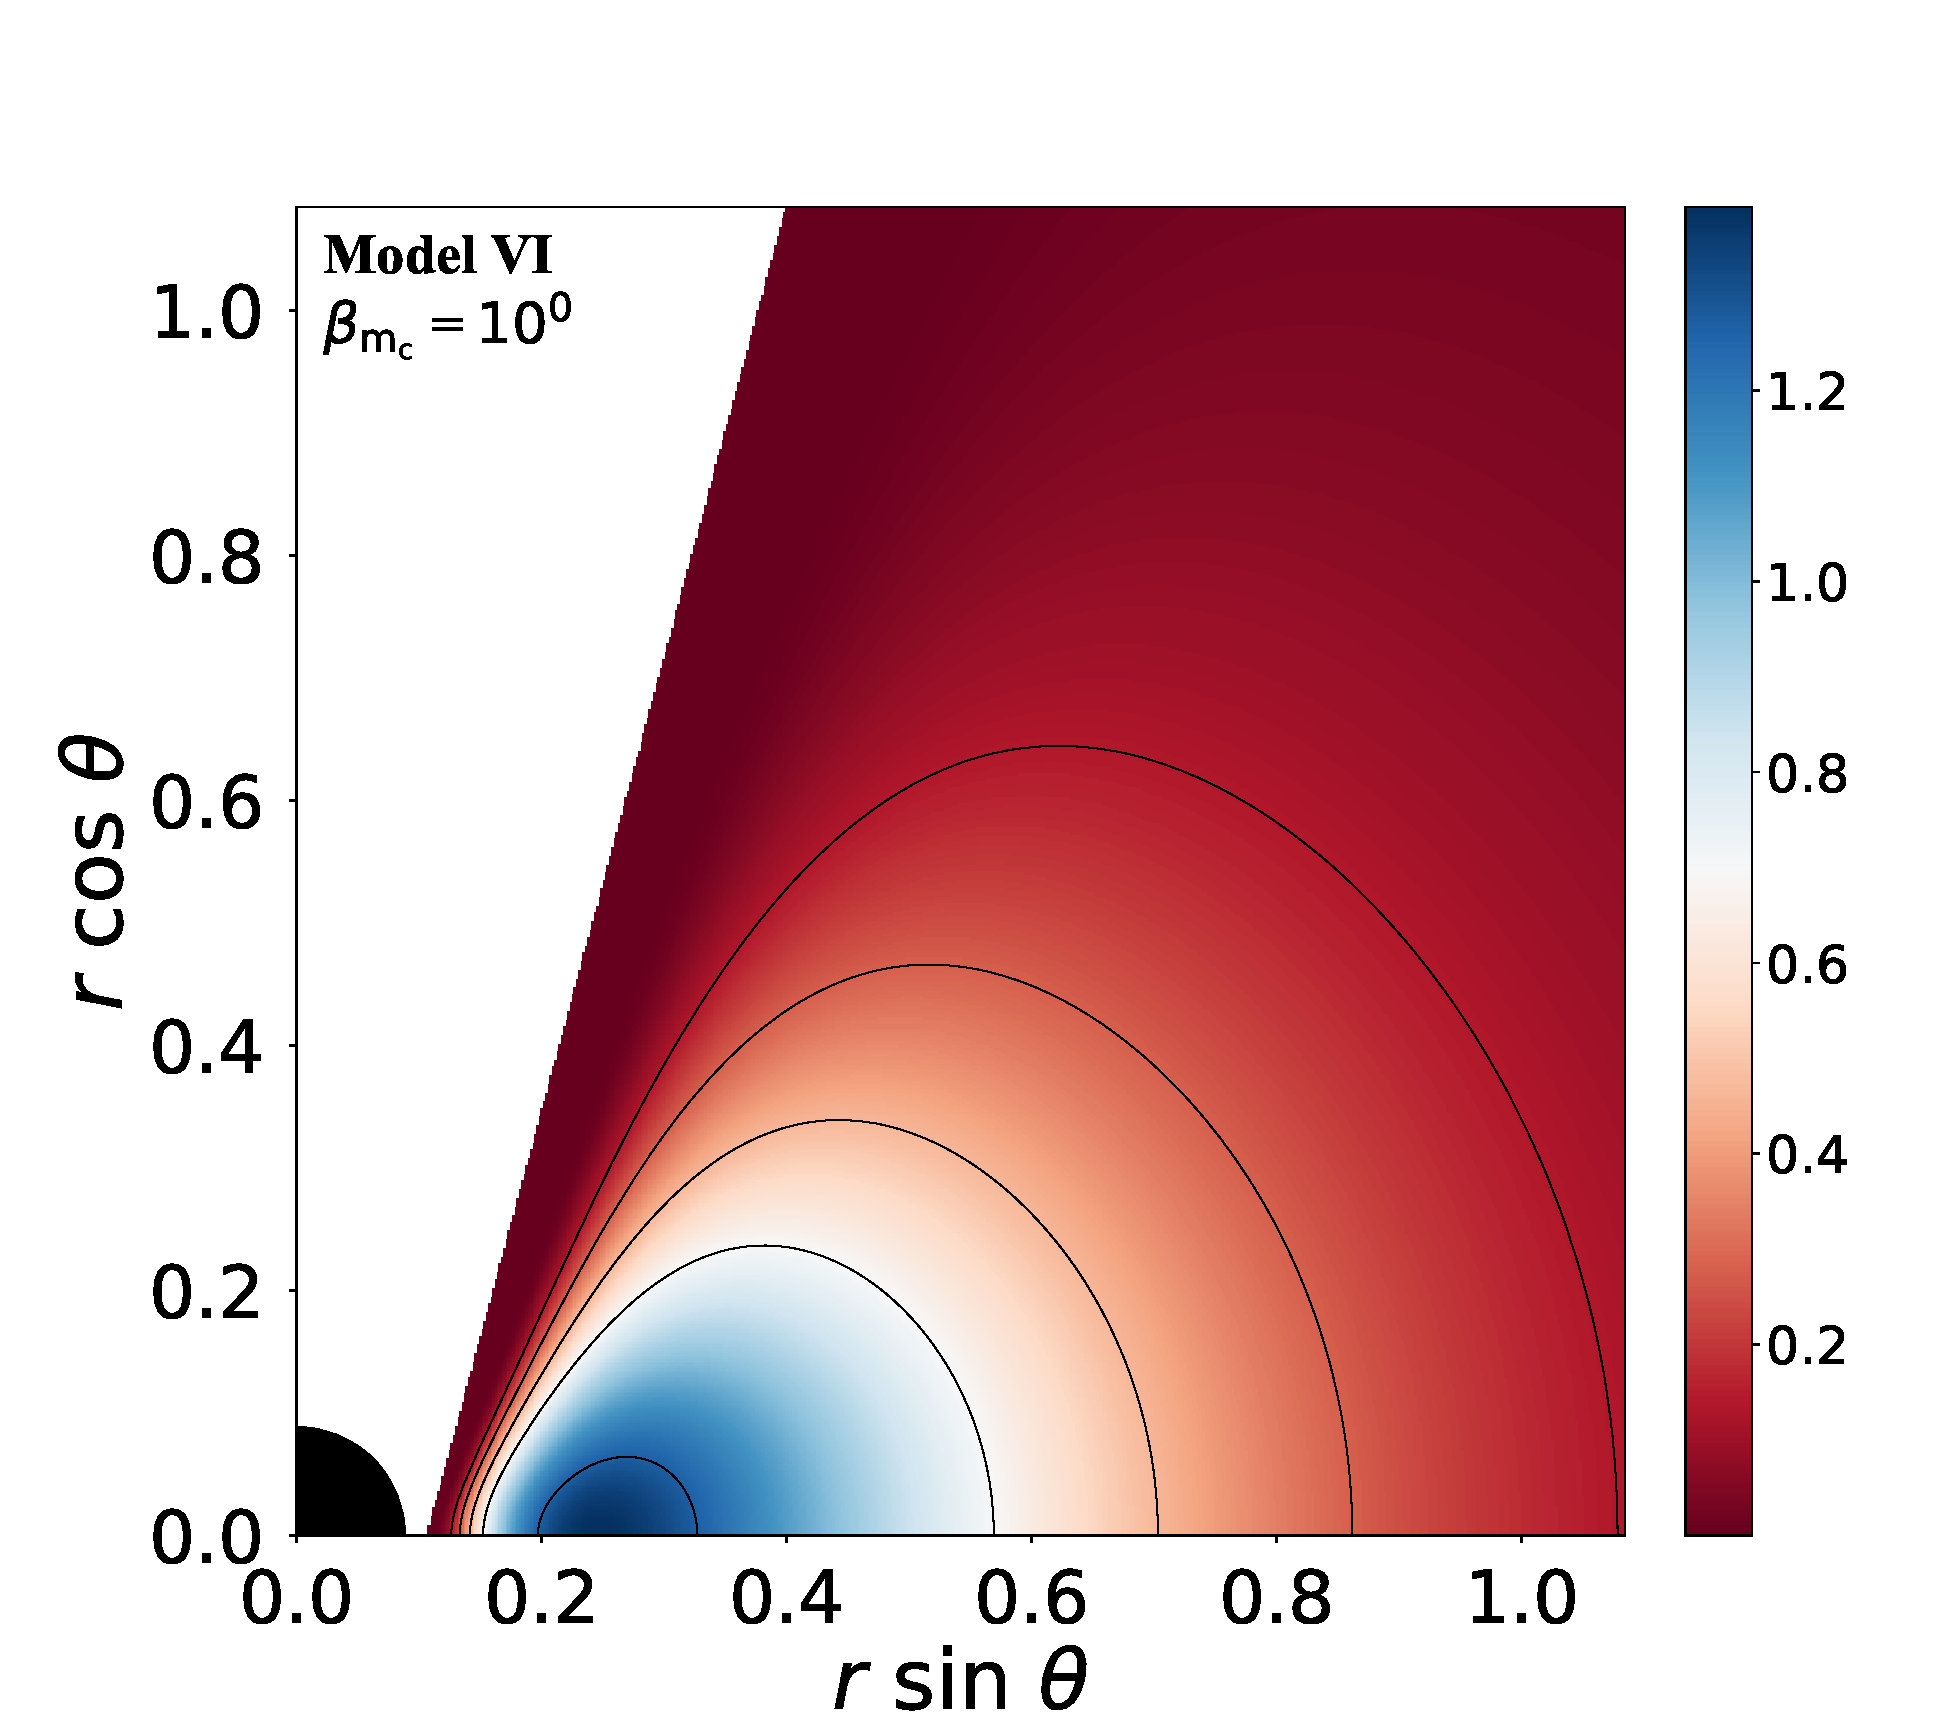
\includegraphics[scale=0.14]{figures/fig2_VI_1.pdf}
\hspace{-0.2cm}
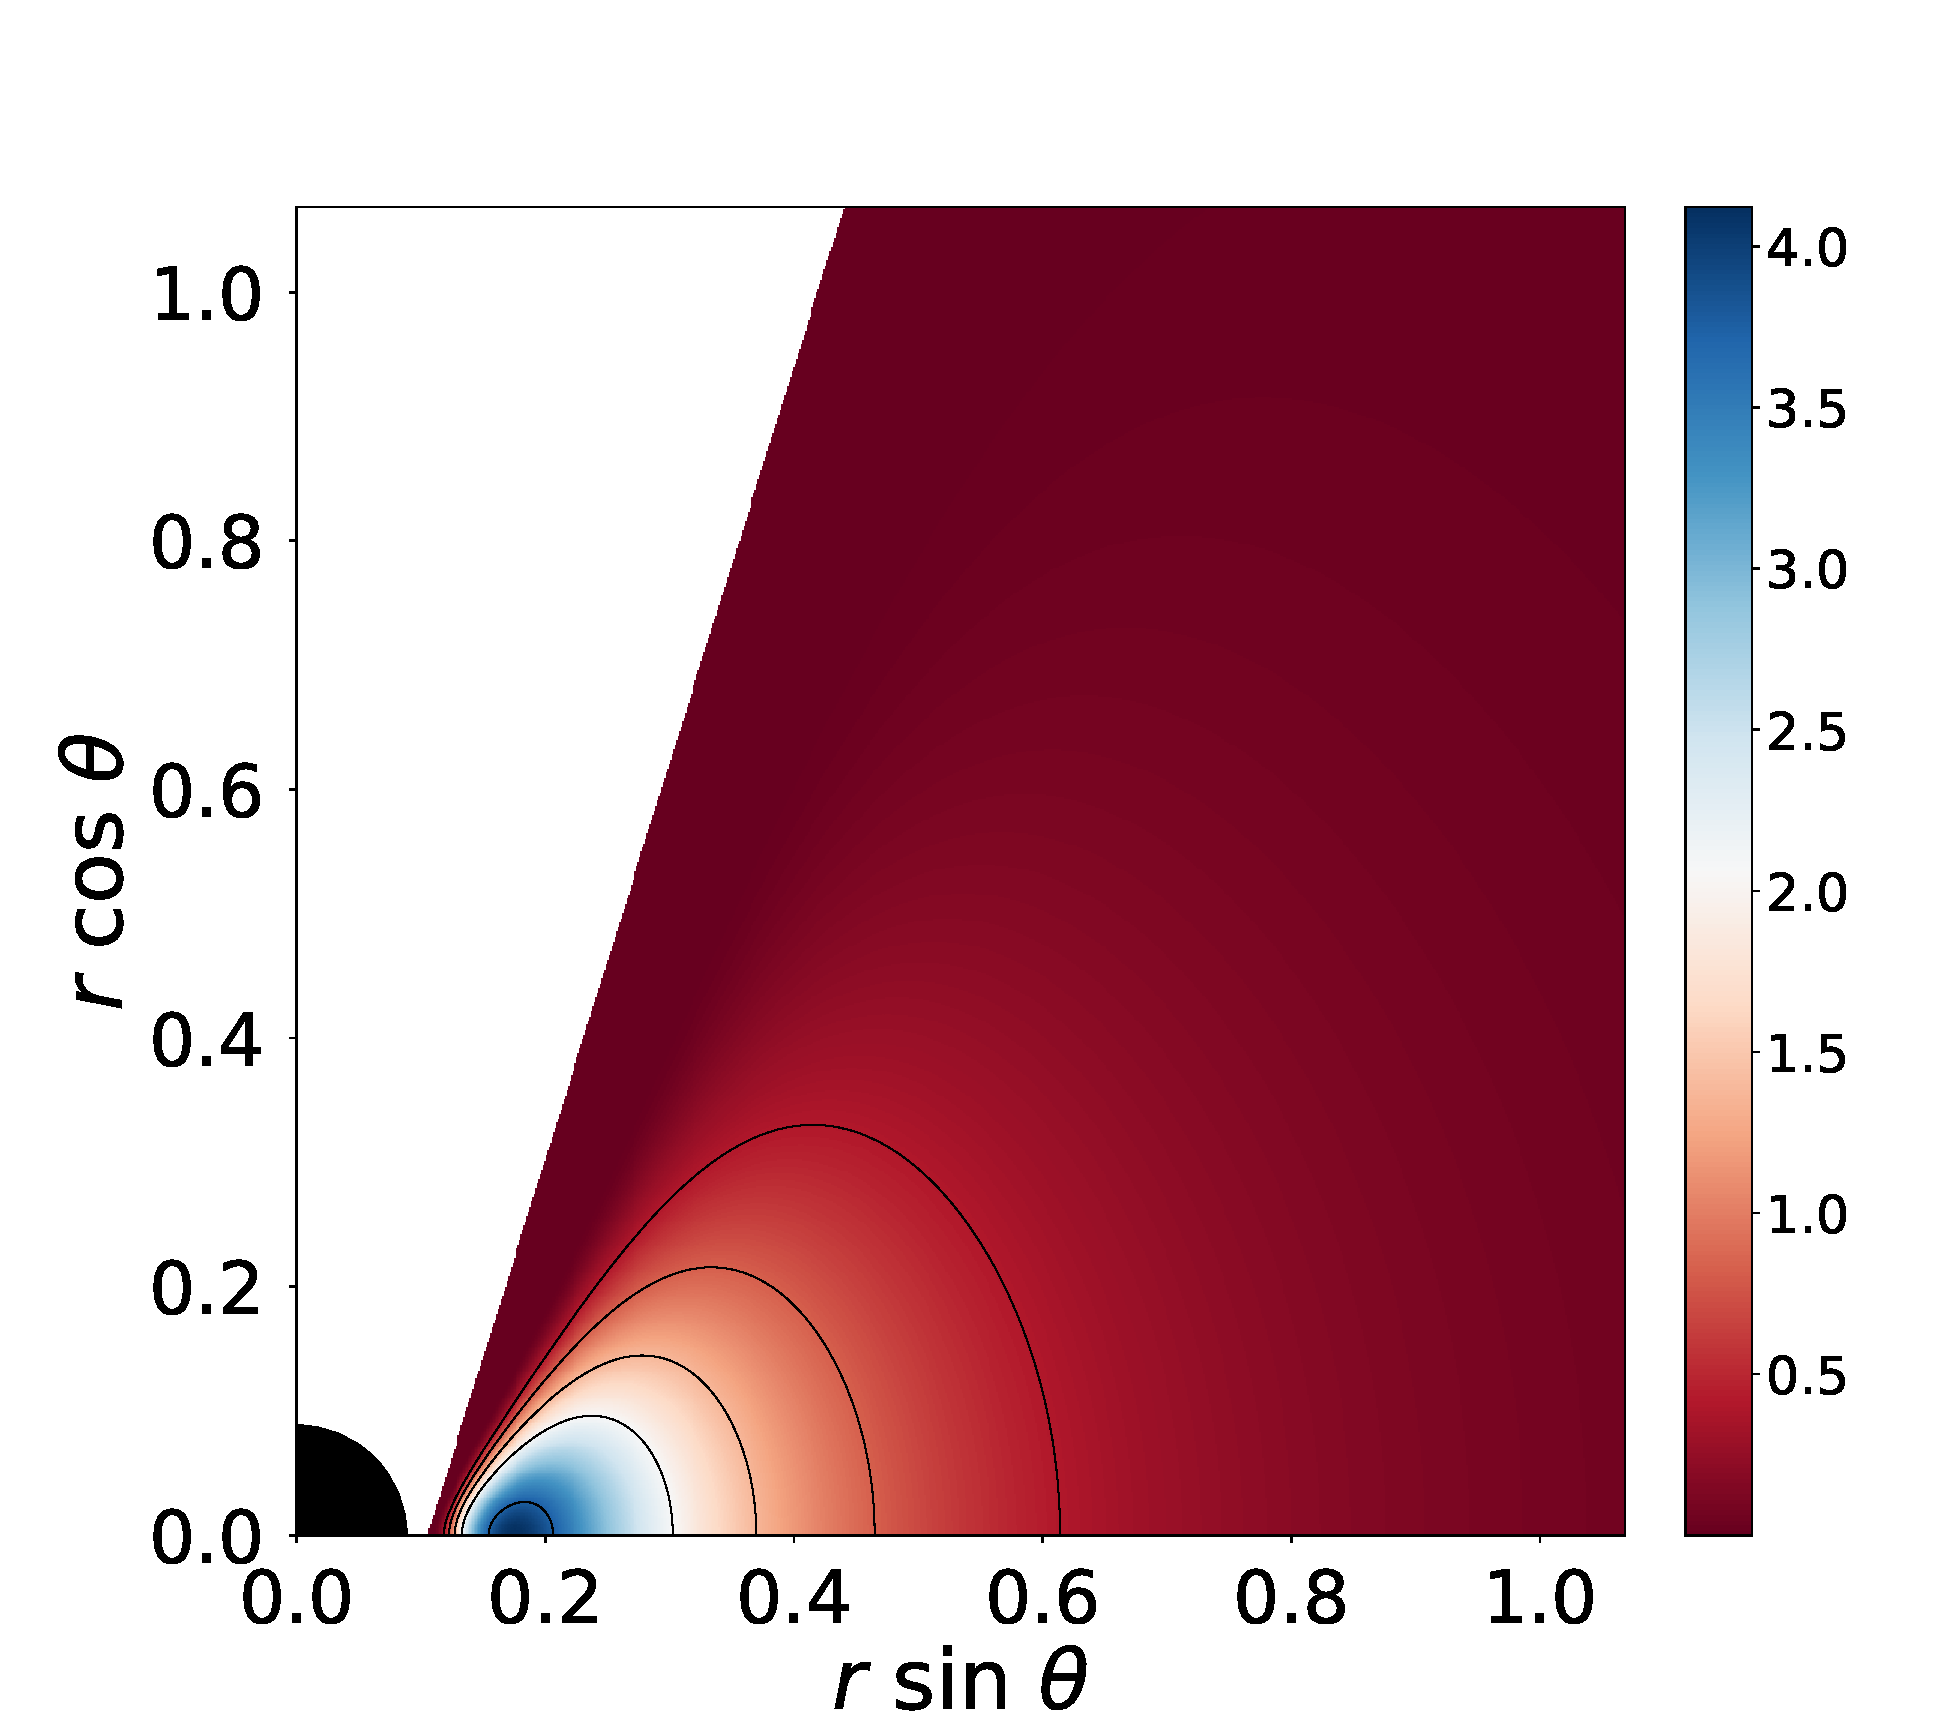
\includegraphics[scale=0.14]{figures/fig2_VI__10.pdf}
\\
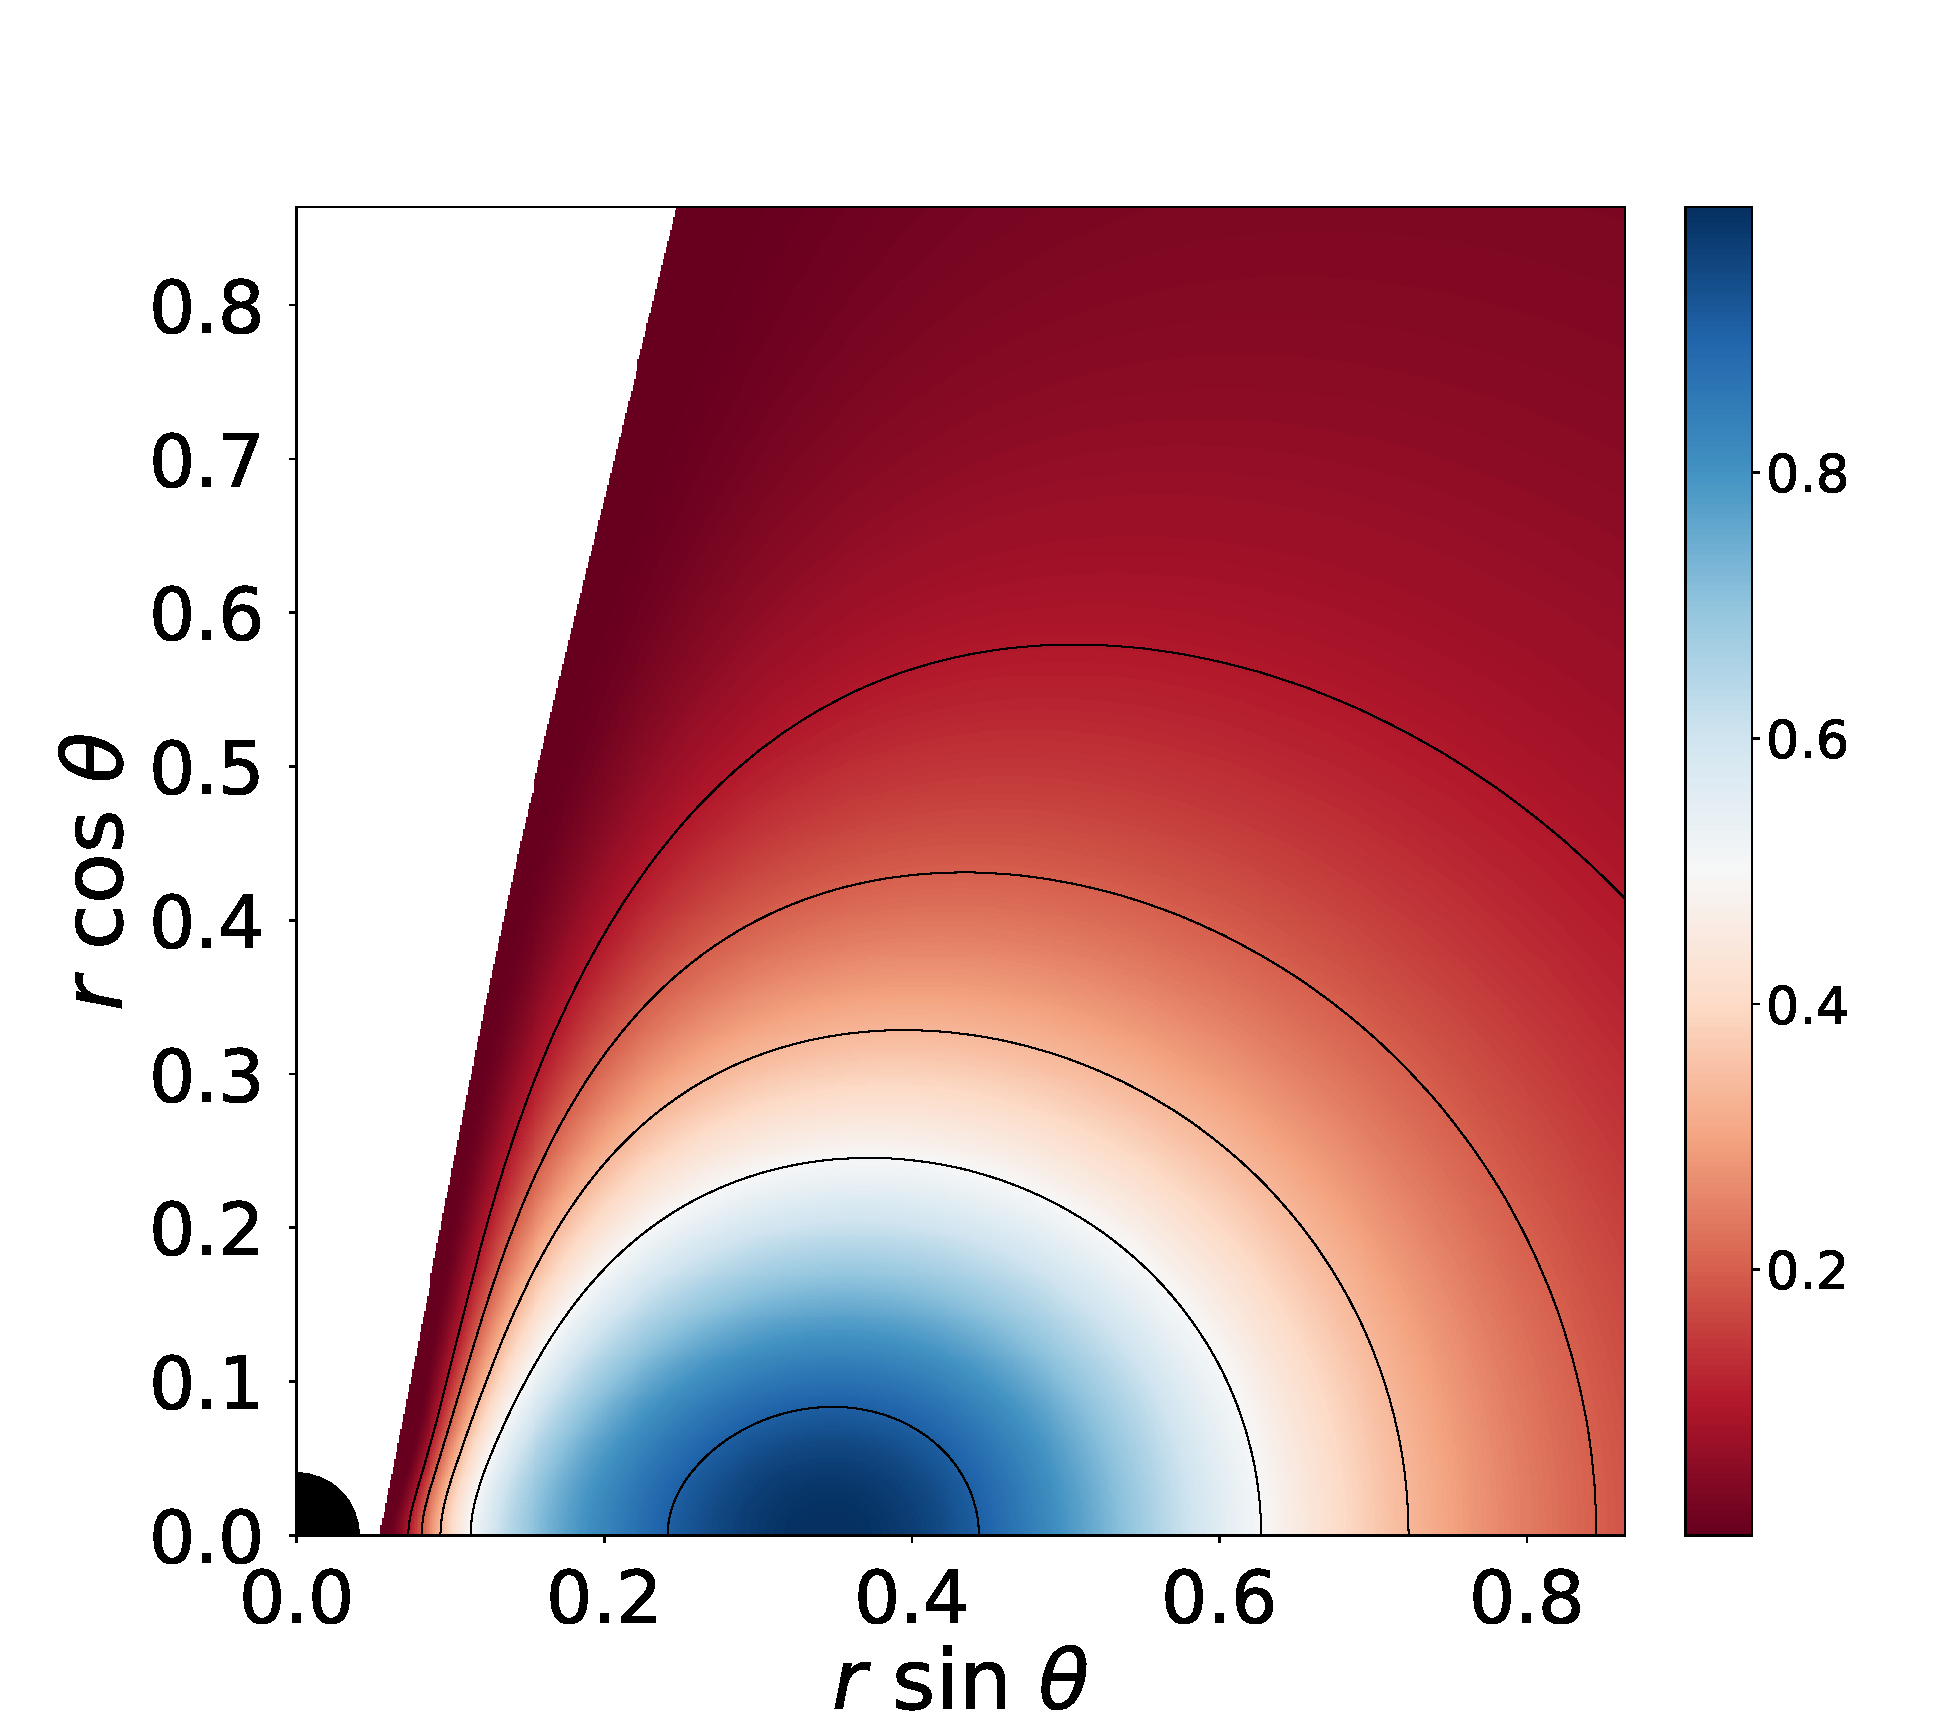
\includegraphics[scale=0.14]{figures/fig2_VII_10.pdf}
\hspace{-0.3cm}
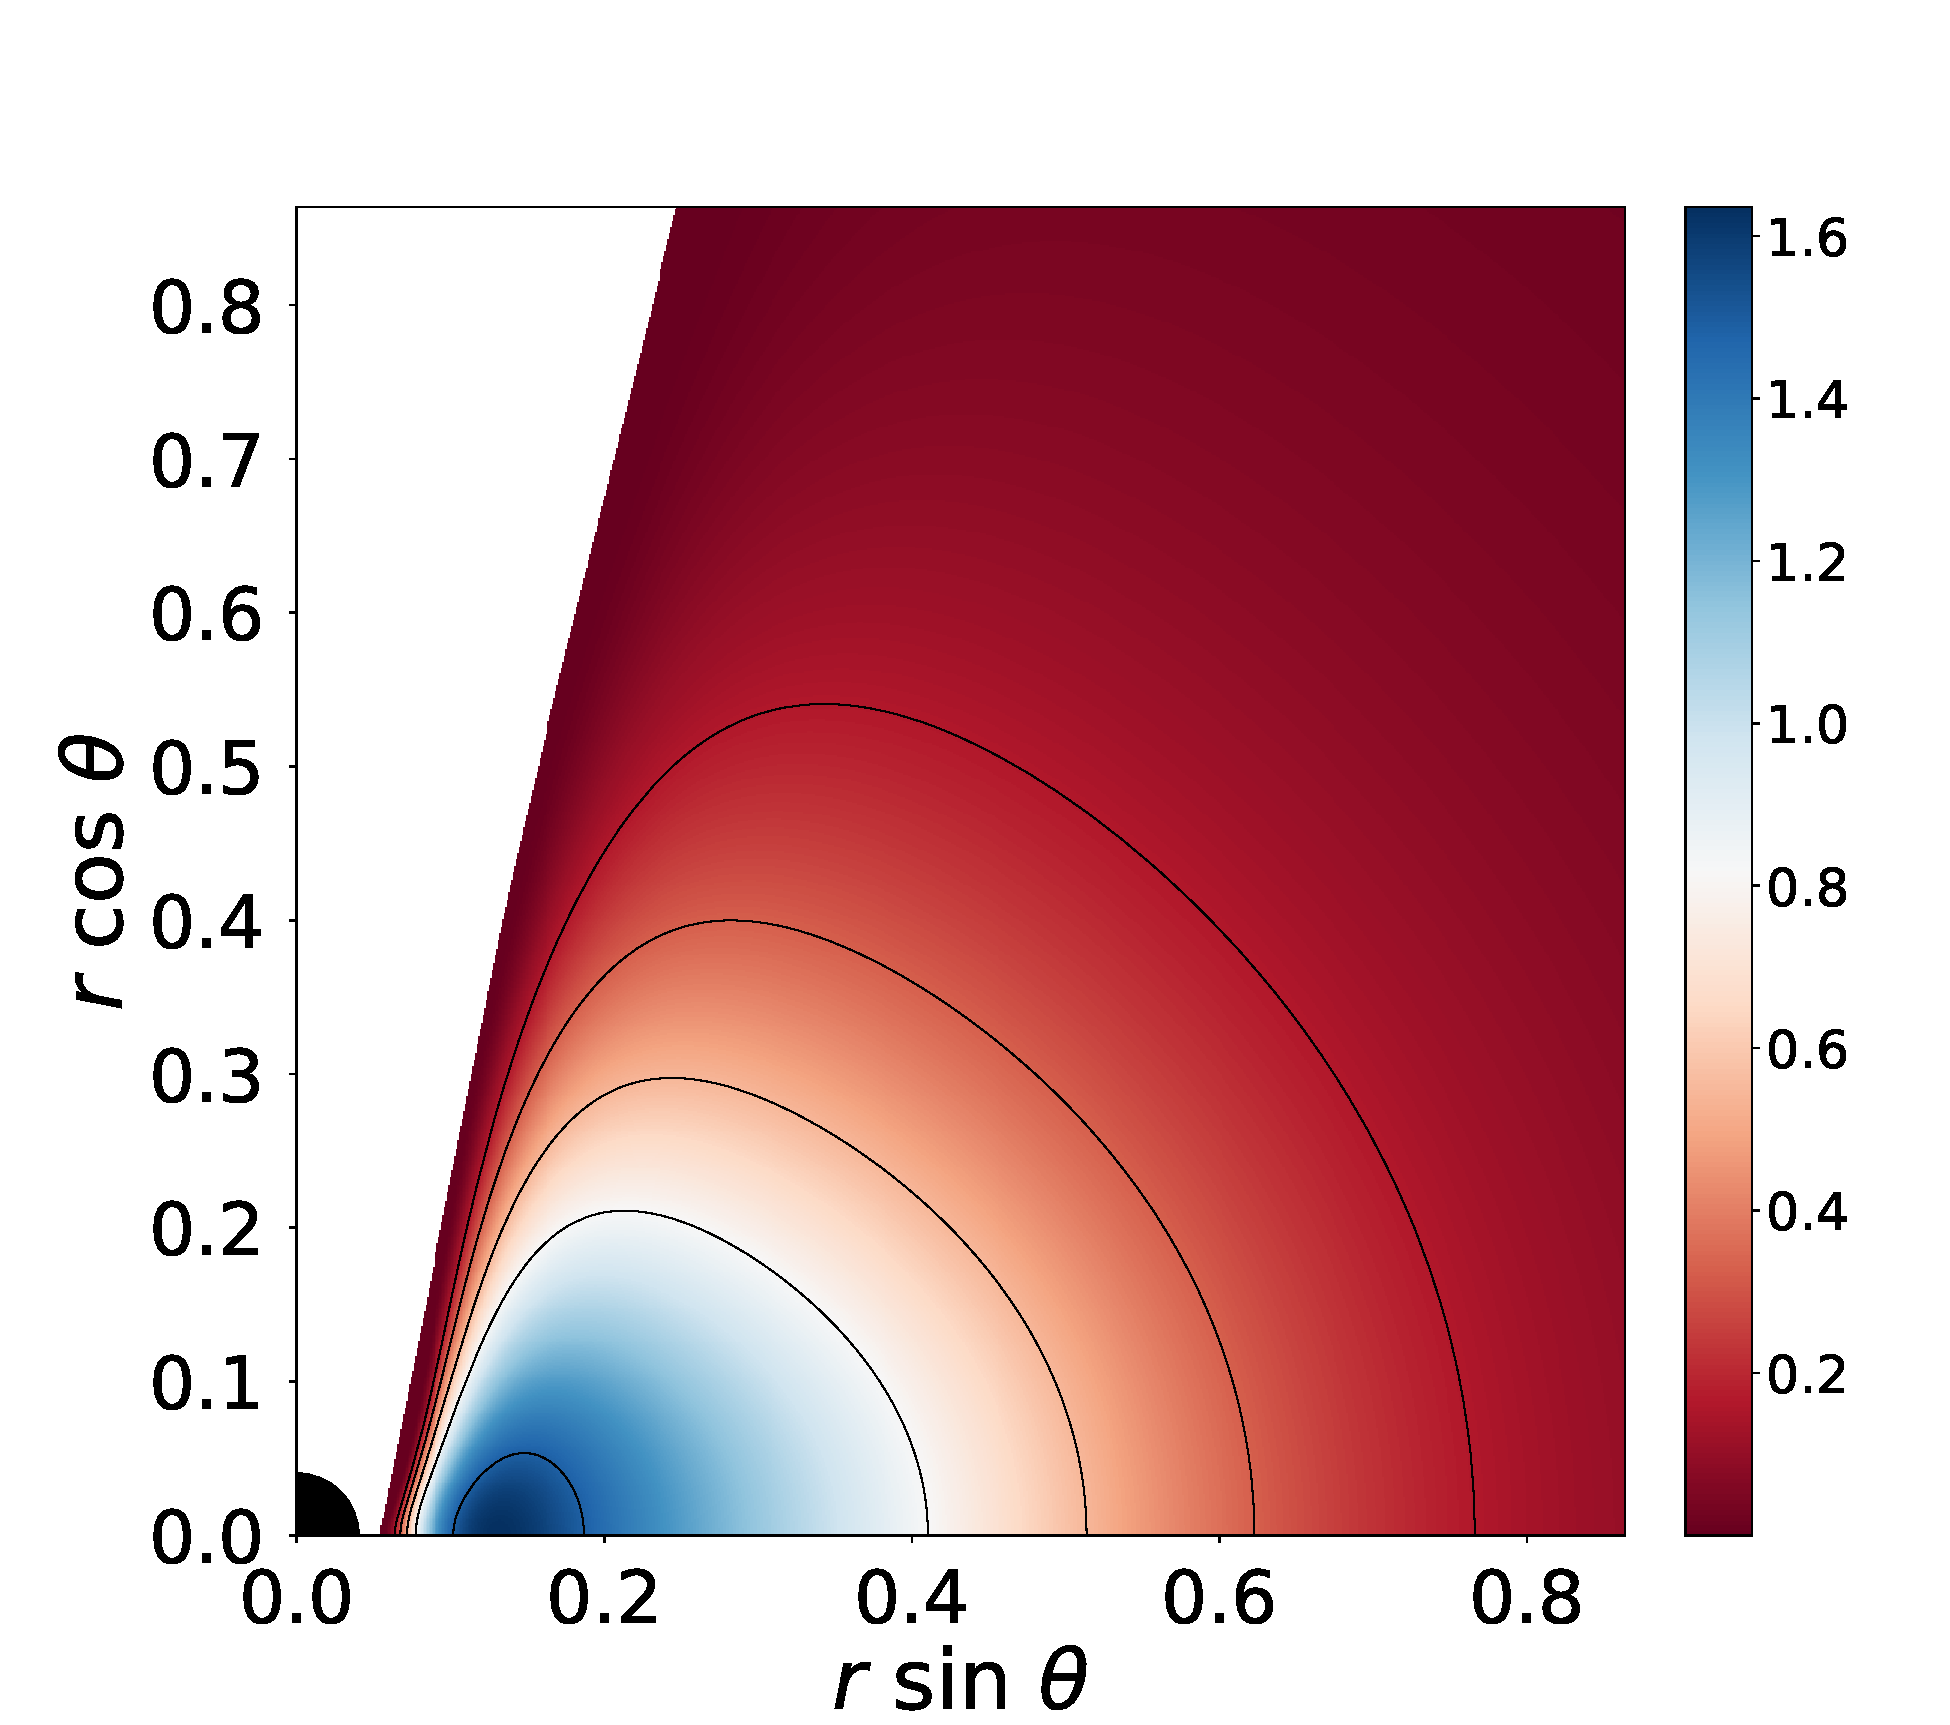
\includegraphics[scale=0.14]{figures/fig2_VII_1.pdf}
\hspace{-0.2cm}
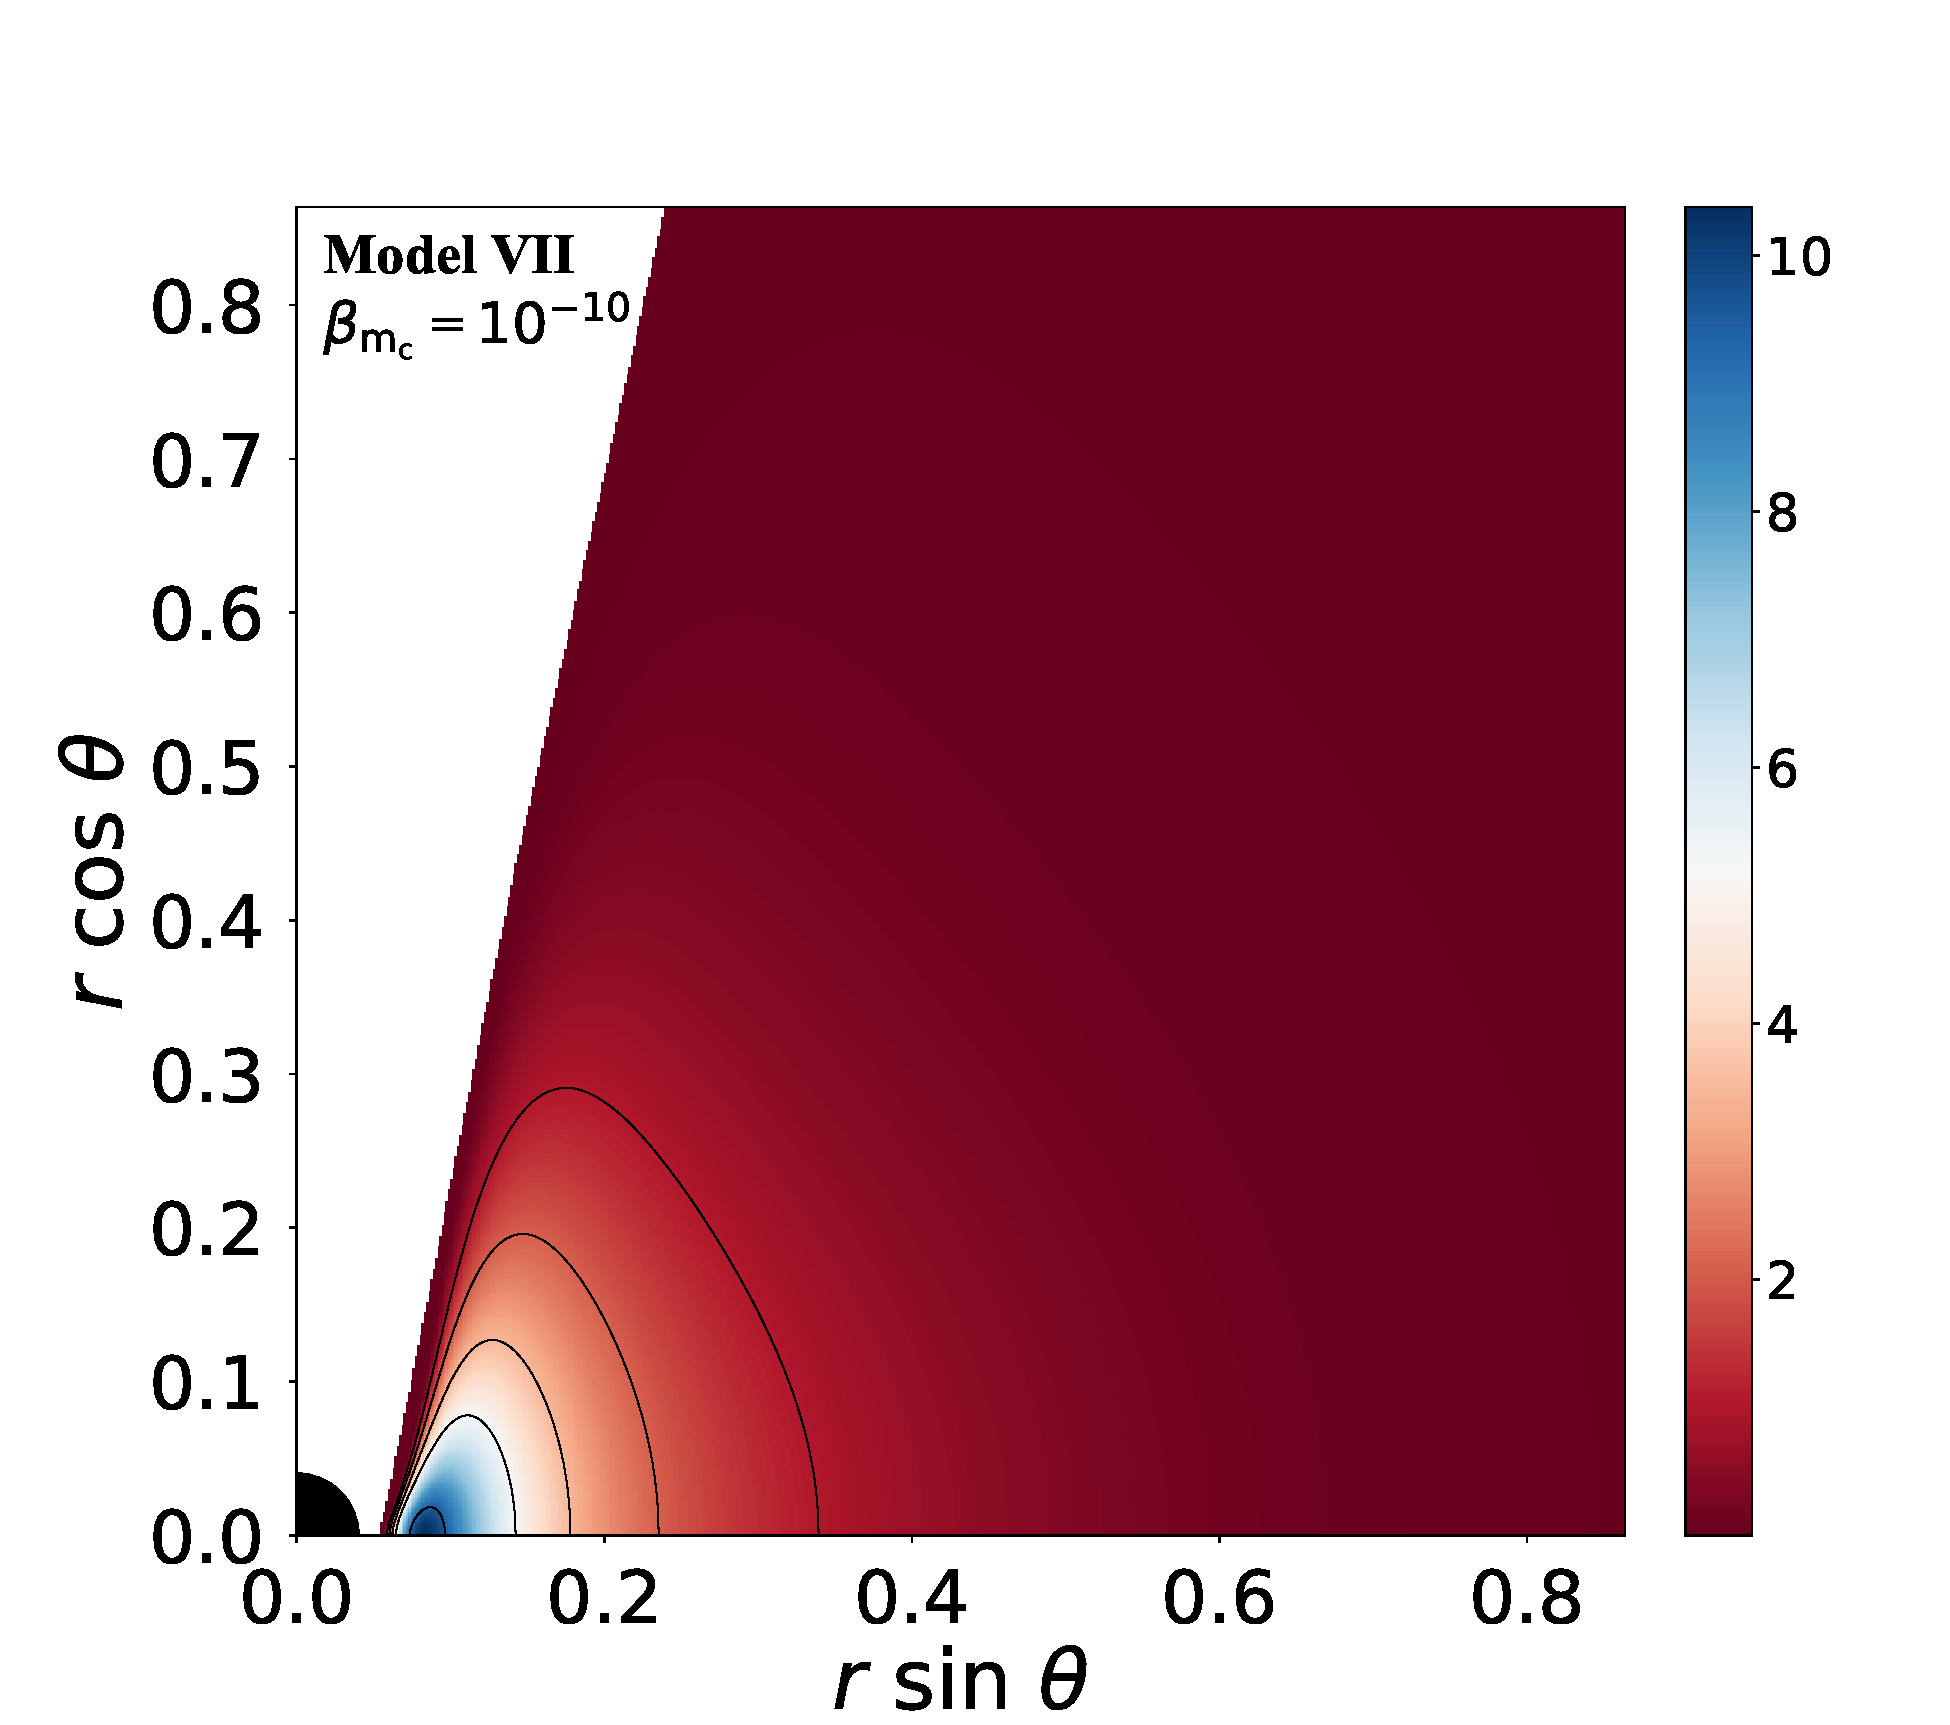
\includegraphics[scale=0.14]{figures/fig2_VII__10.pdf}
\hspace{-0.2cm}
\caption{Same as Fig.~\ref{models_I} but for the last three models of KBHsSH (V, VI, and VII). \tf{Same comment as in the previous figure.}}
\label{models_II}
\end{figure*}

\begin{figure*}
\centering
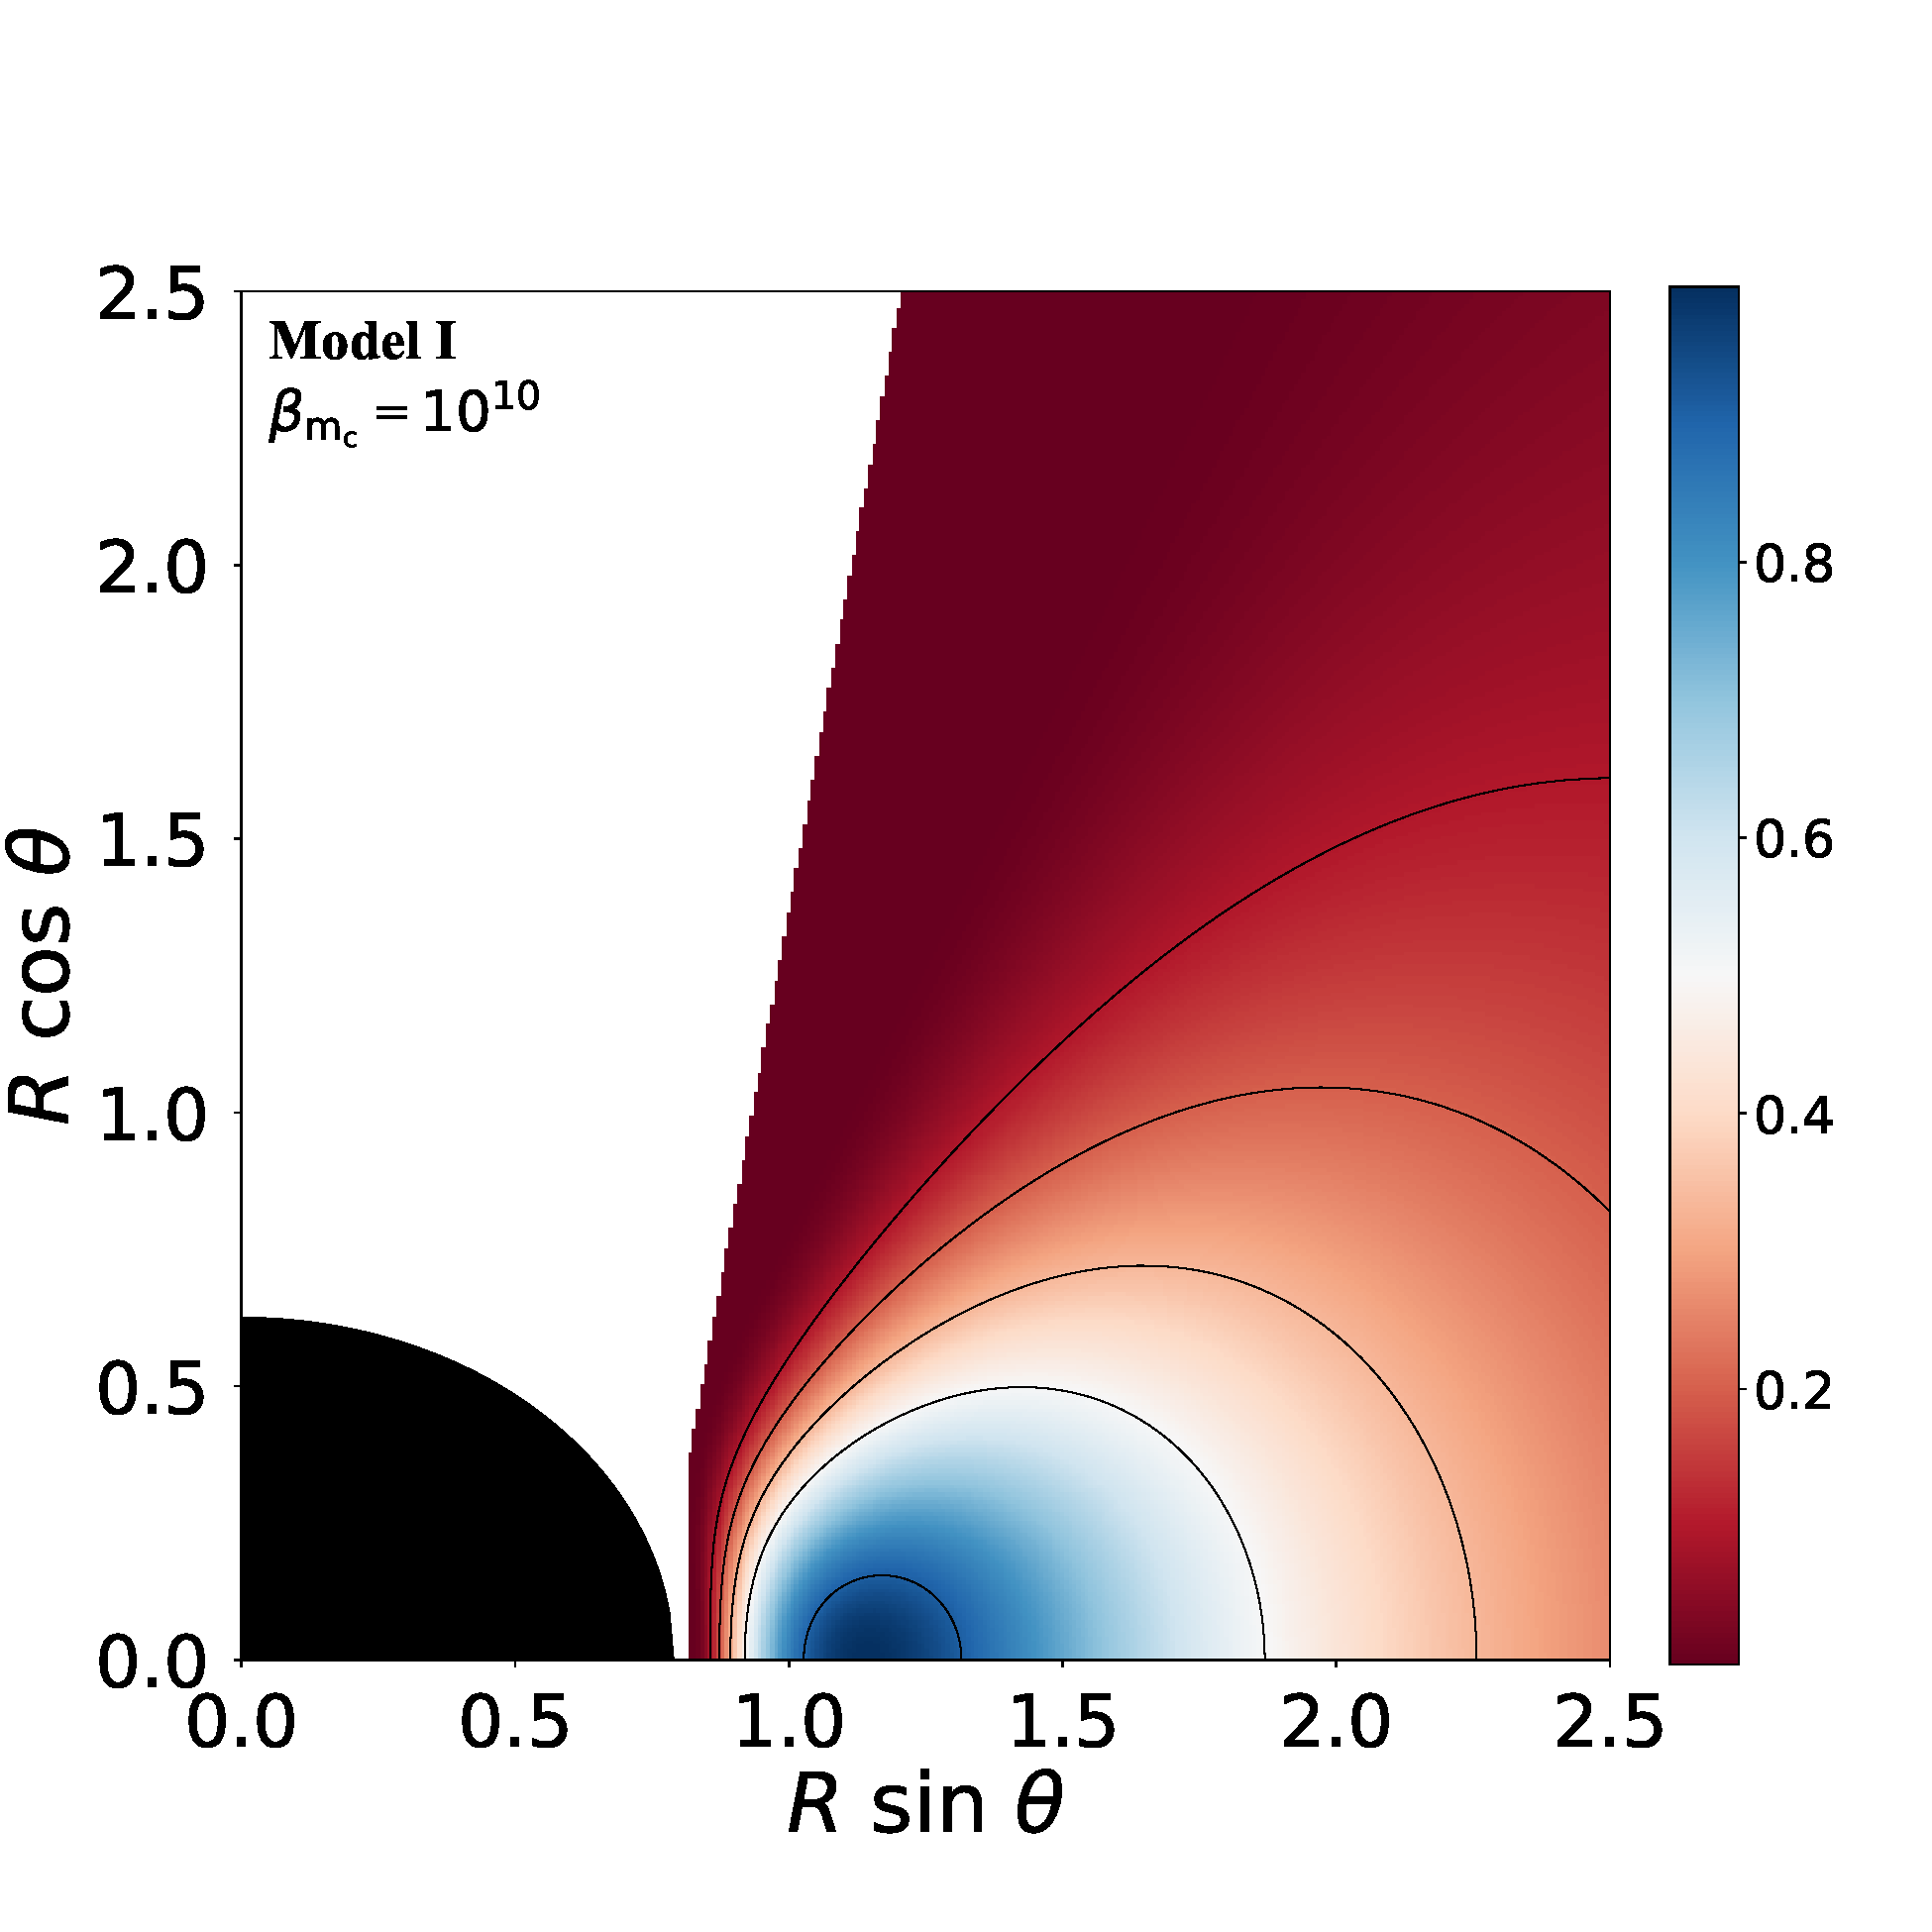
\includegraphics[scale=0.14]{figures/fig3_I_10.pdf}
\hspace{-0.3cm}
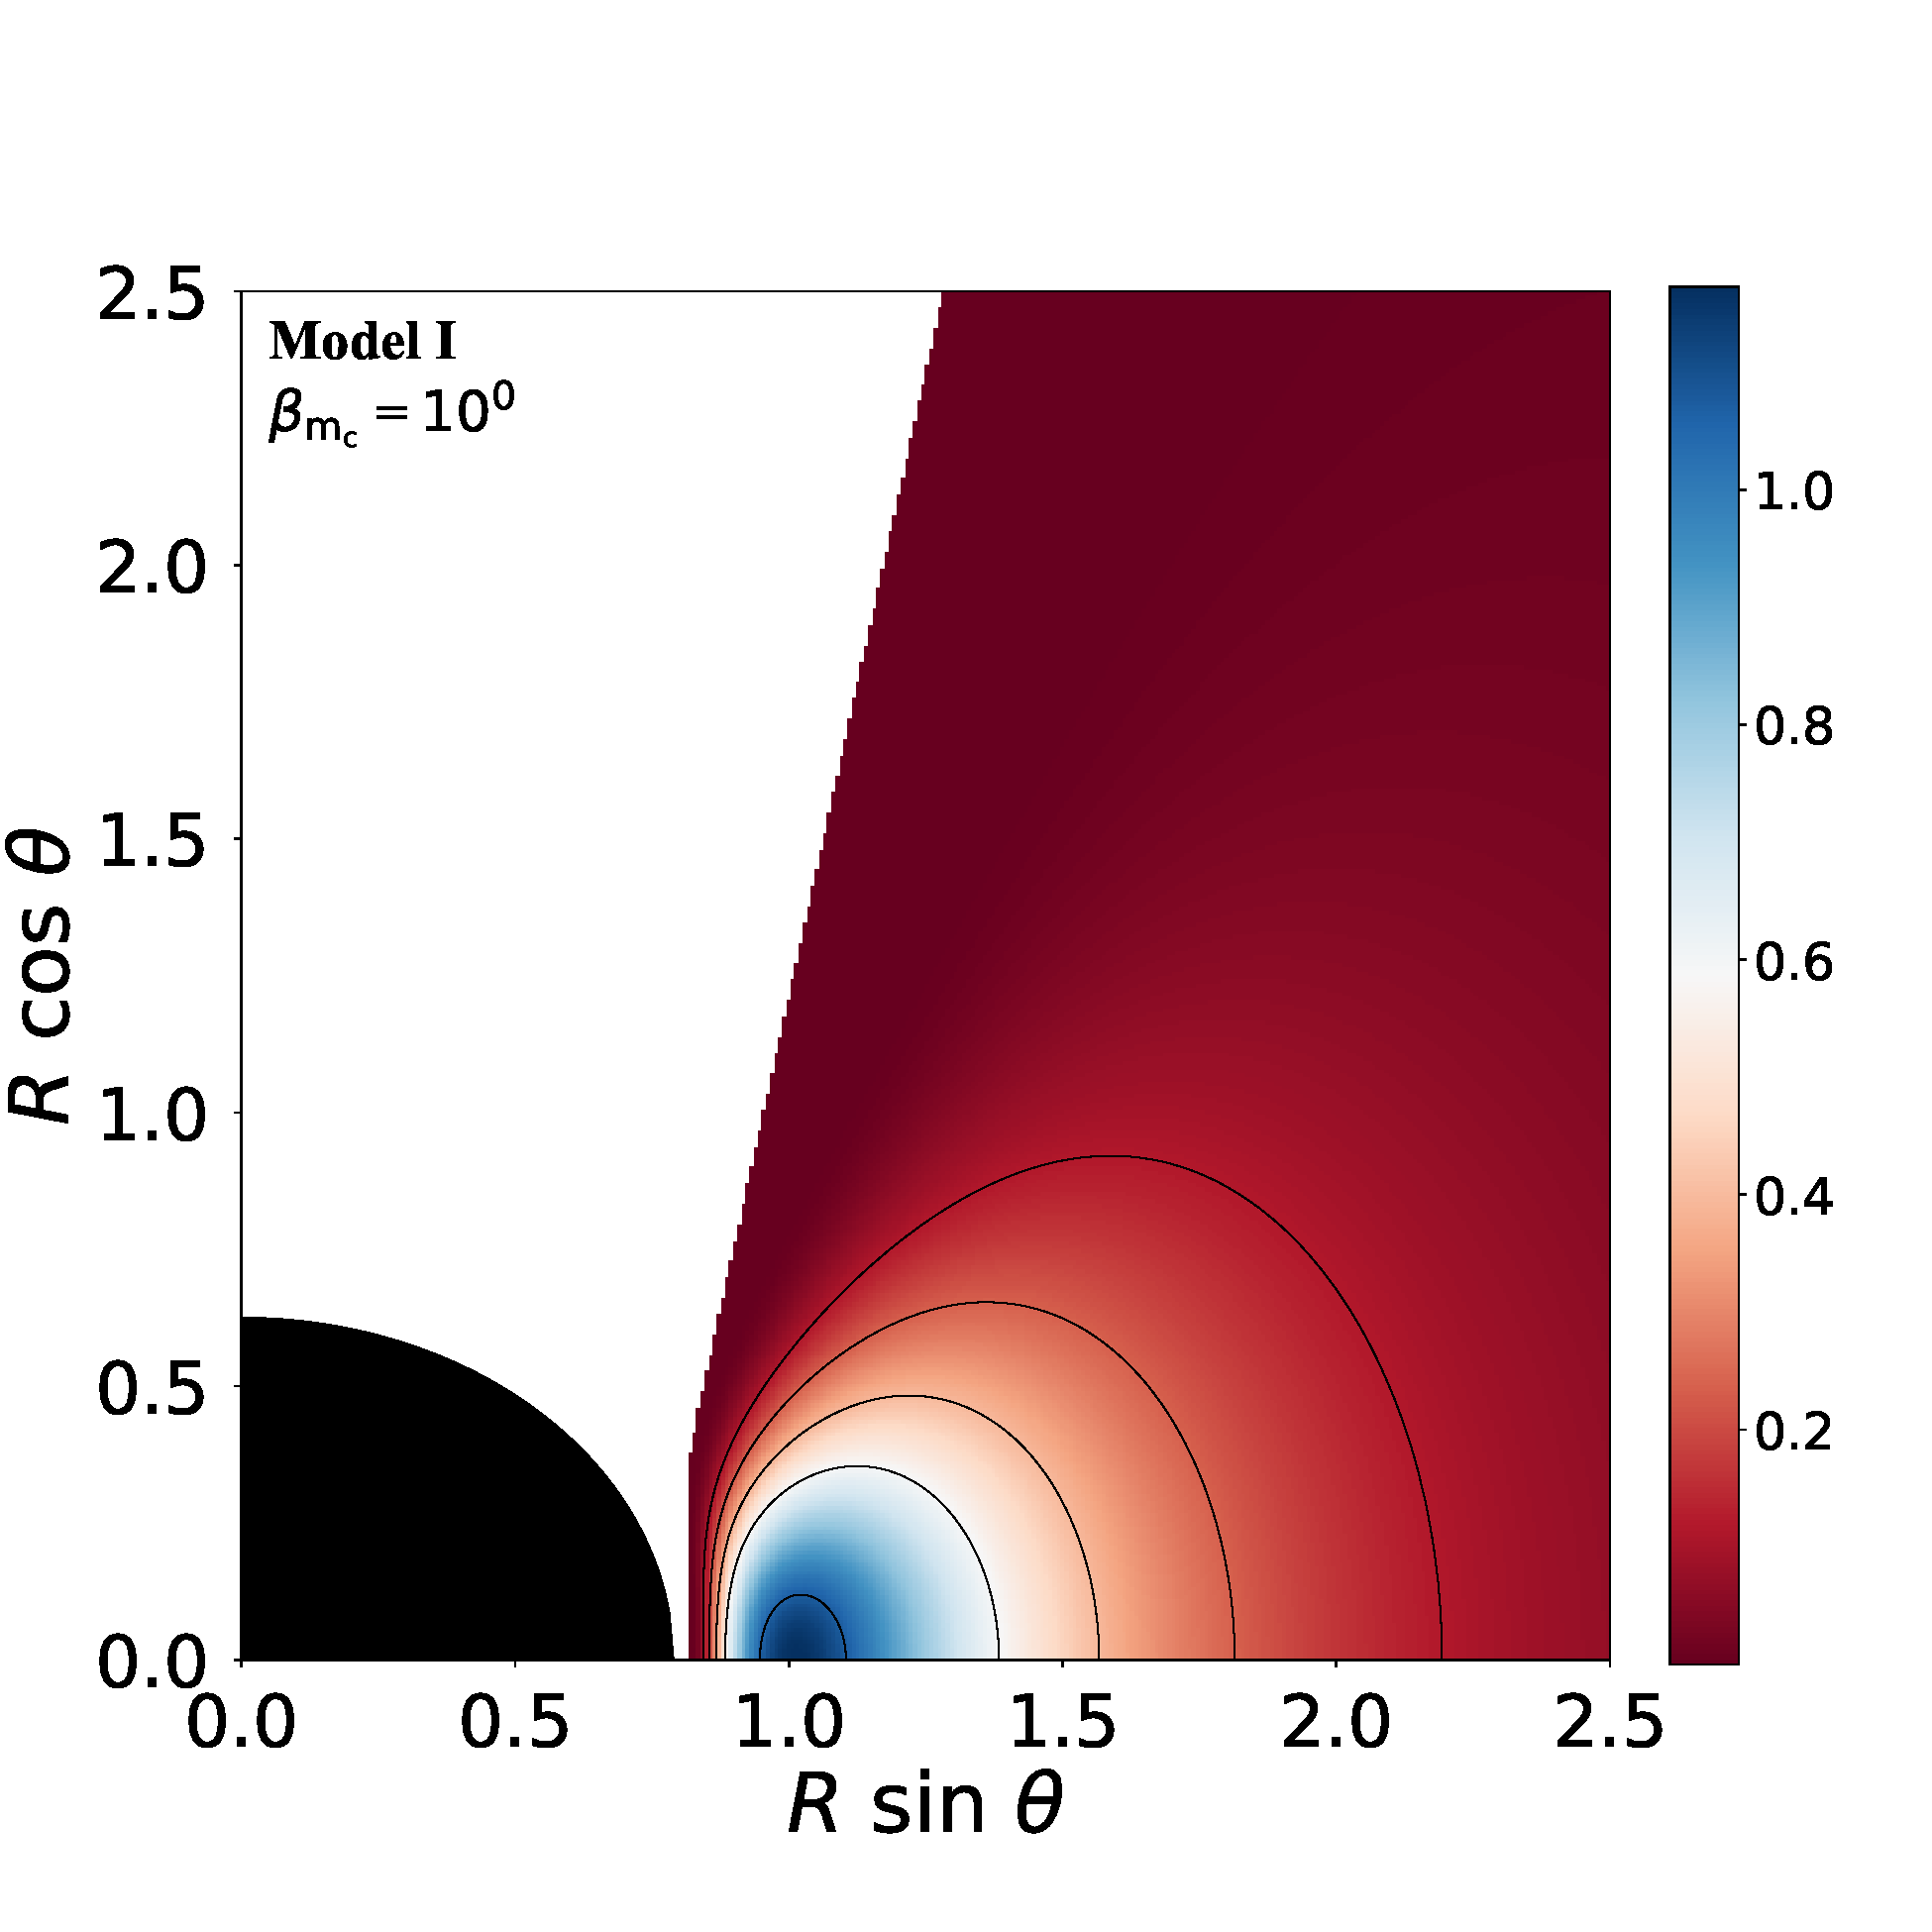
\includegraphics[scale=0.14]{figures/fig3_I_1.pdf}
\hspace{-0.2cm}
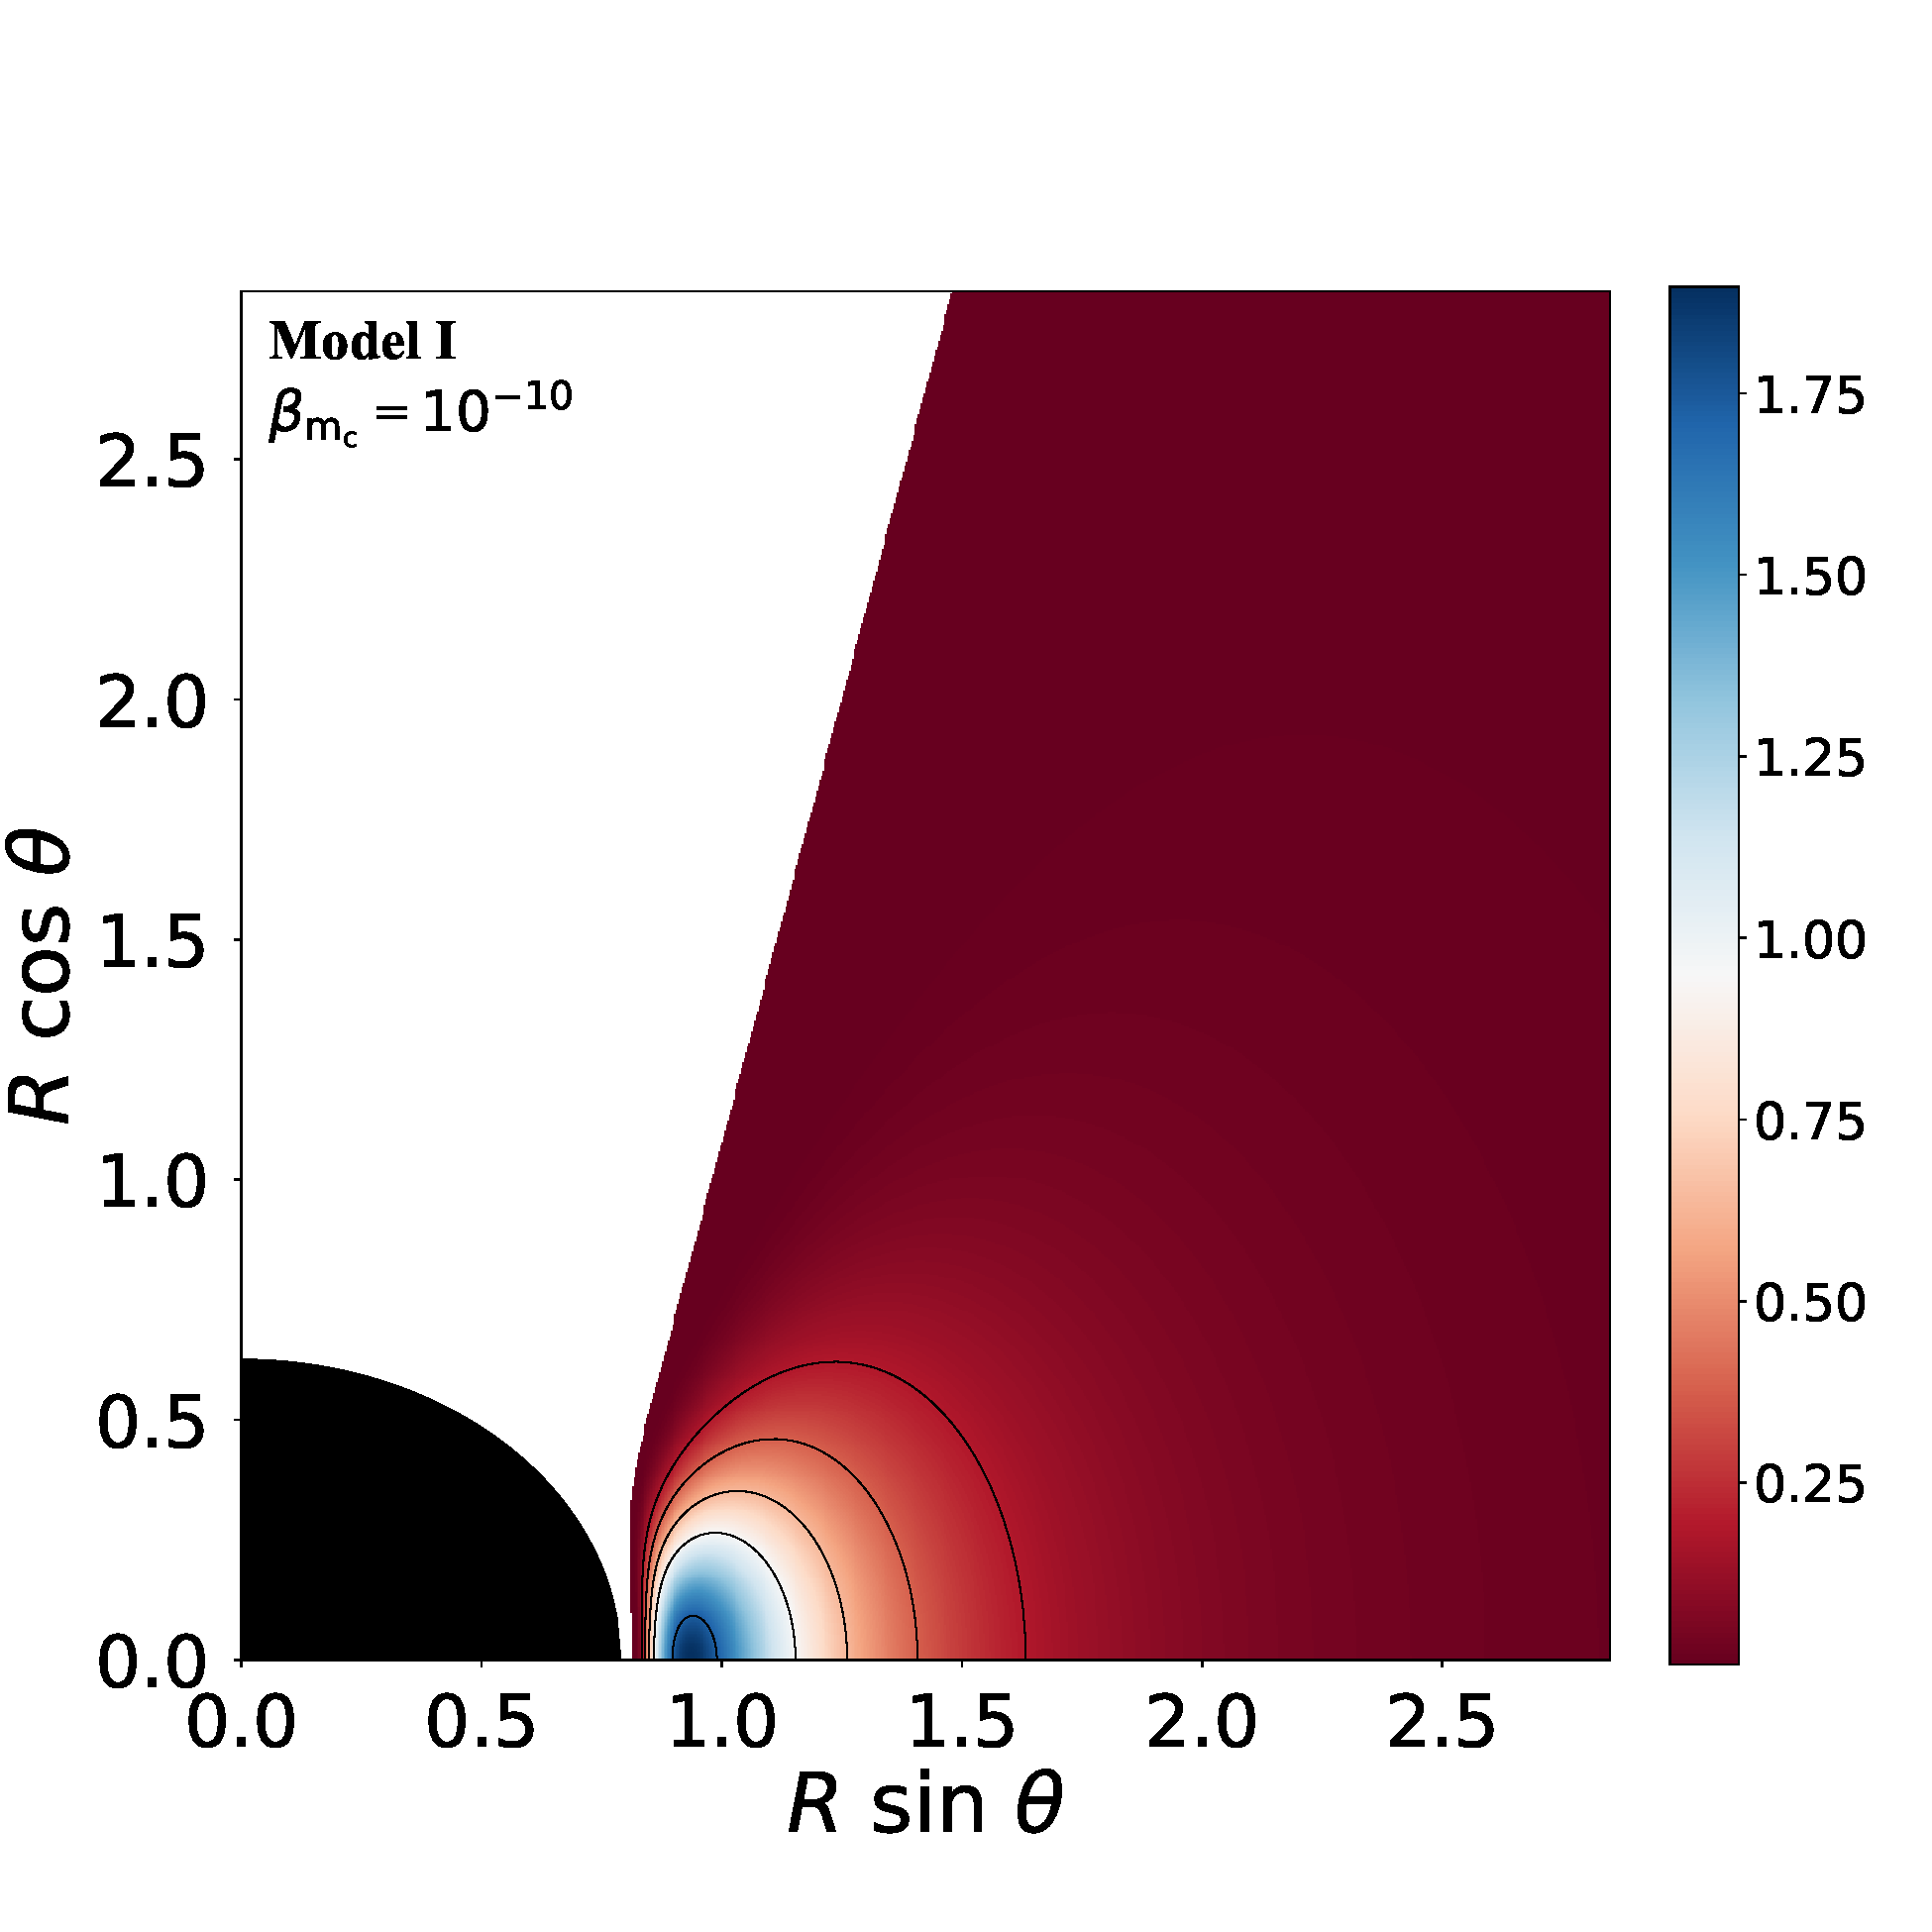
\includegraphics[scale=0.14]{figures/fig3_I__10.pdf}
\\
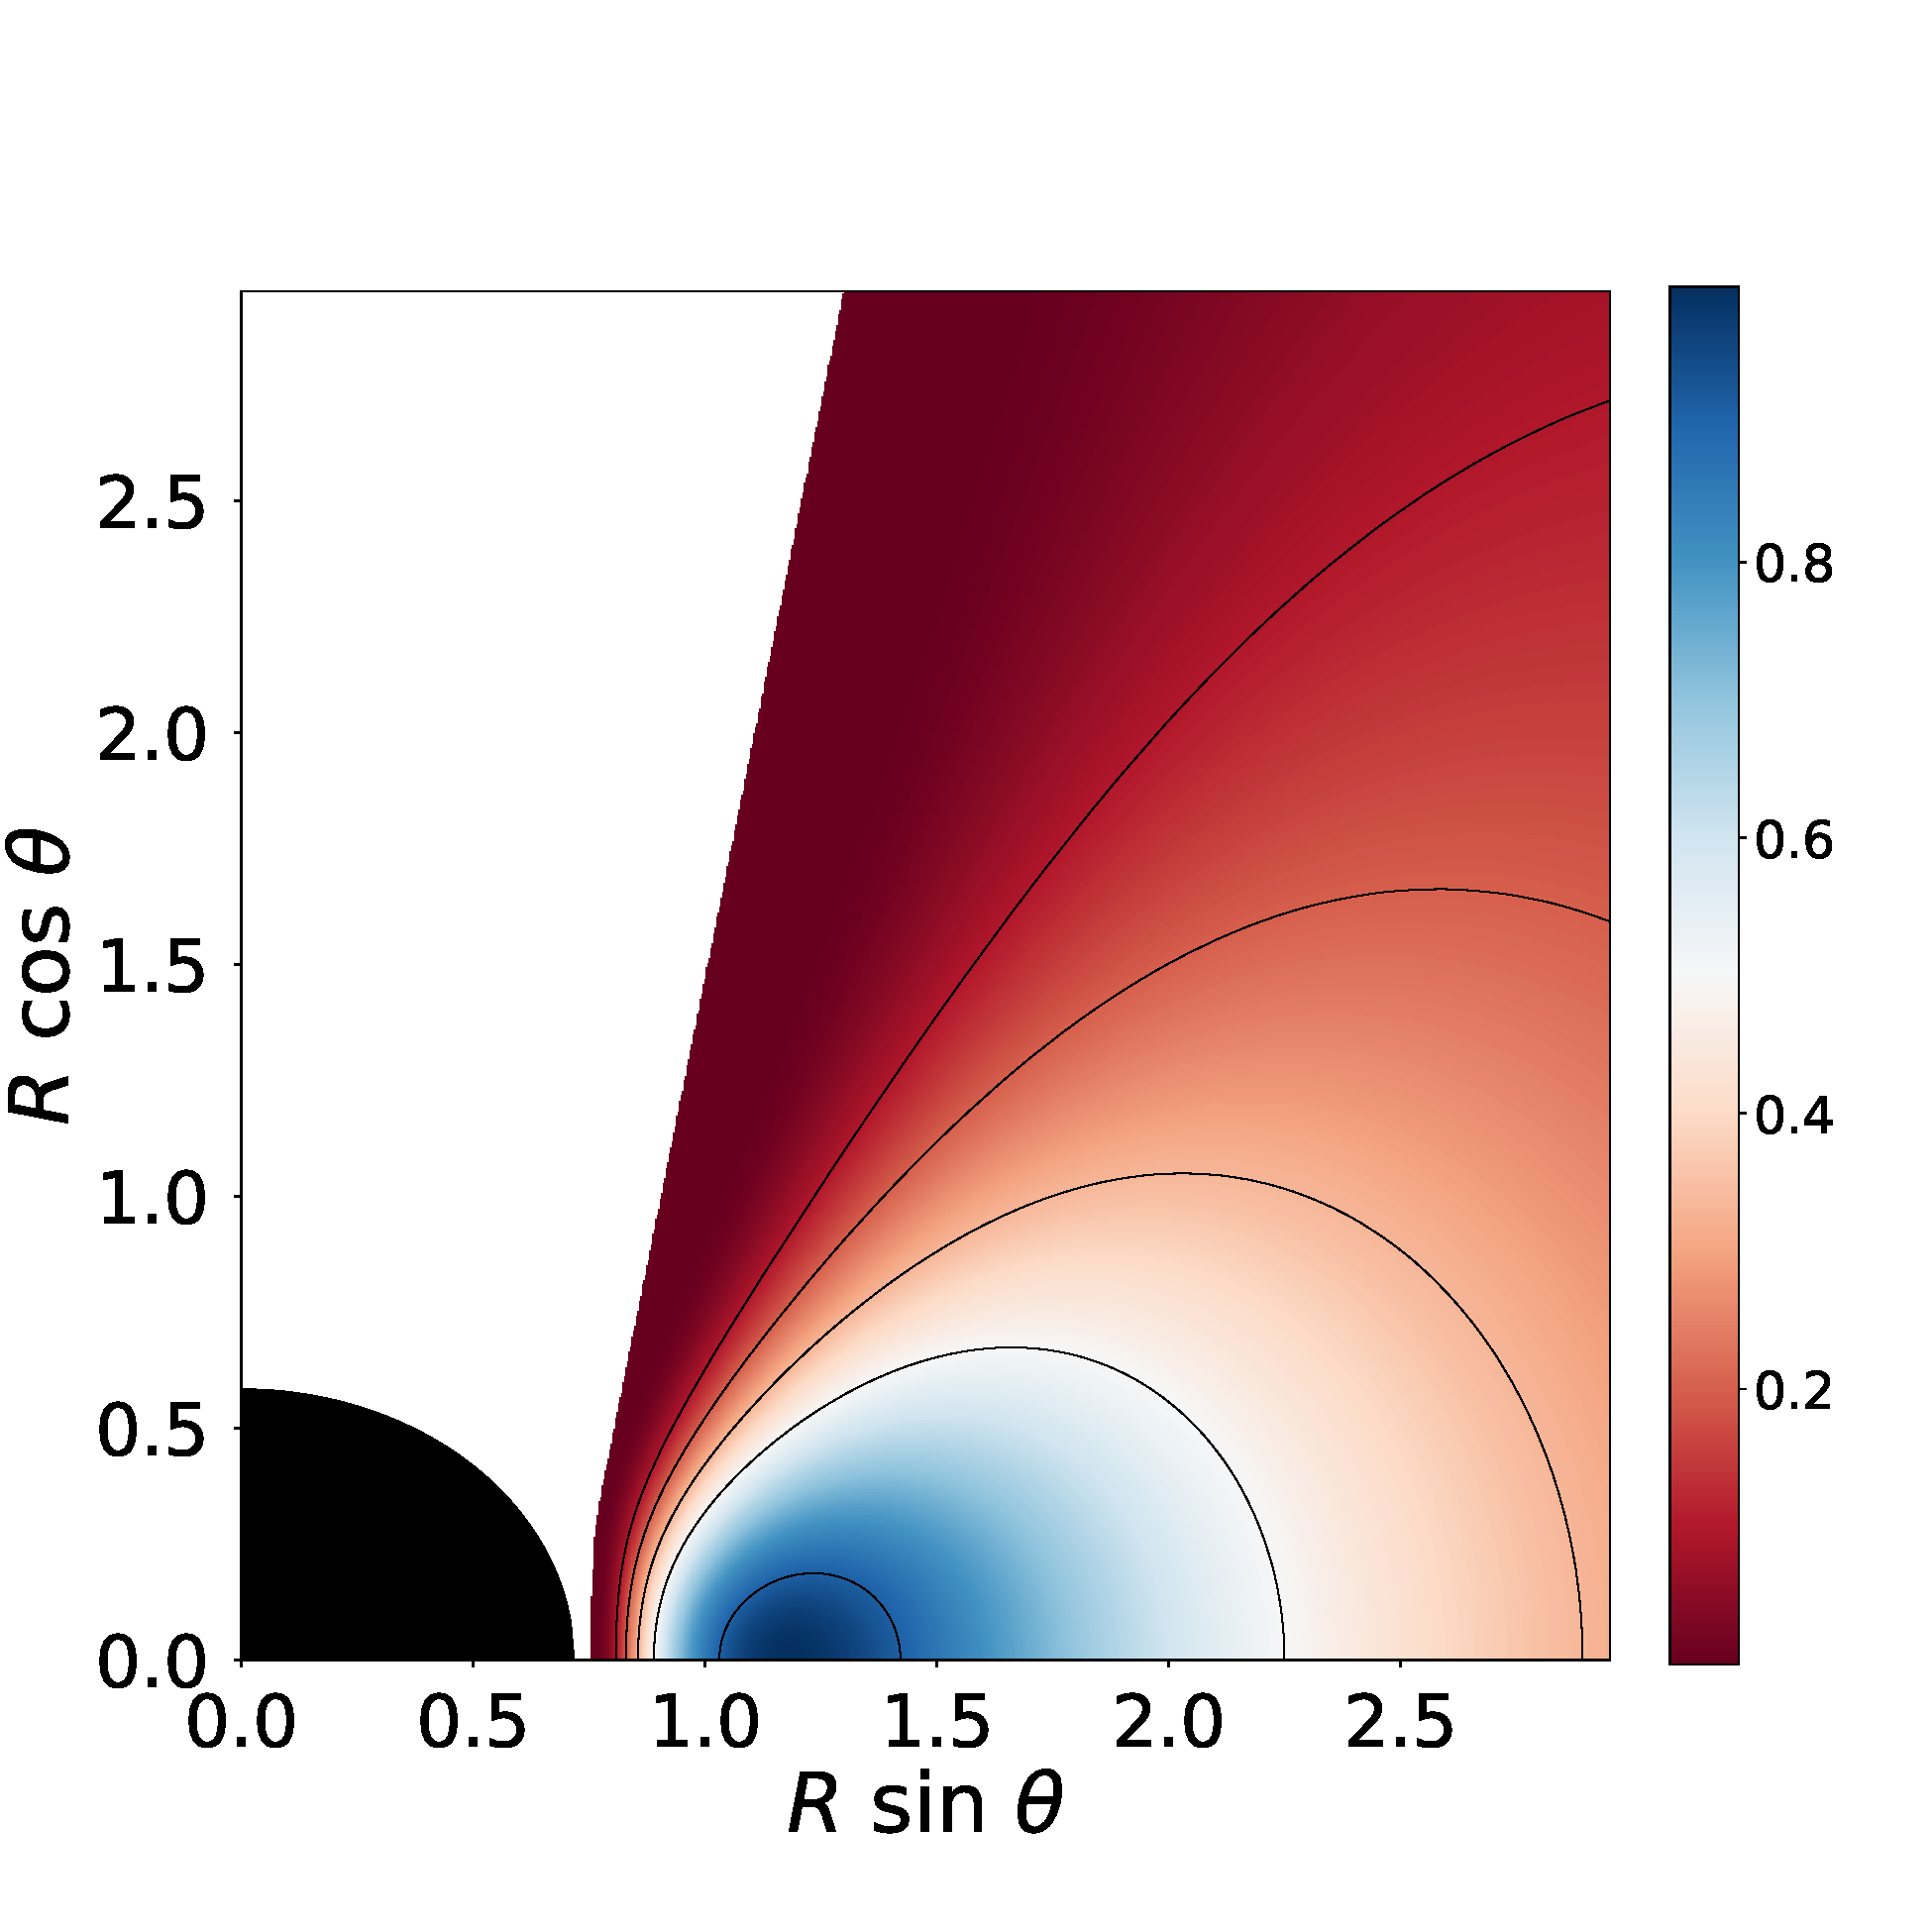
\includegraphics[scale=0.14]{figures/fig3_II_10.pdf}
\hspace{-0.3cm}
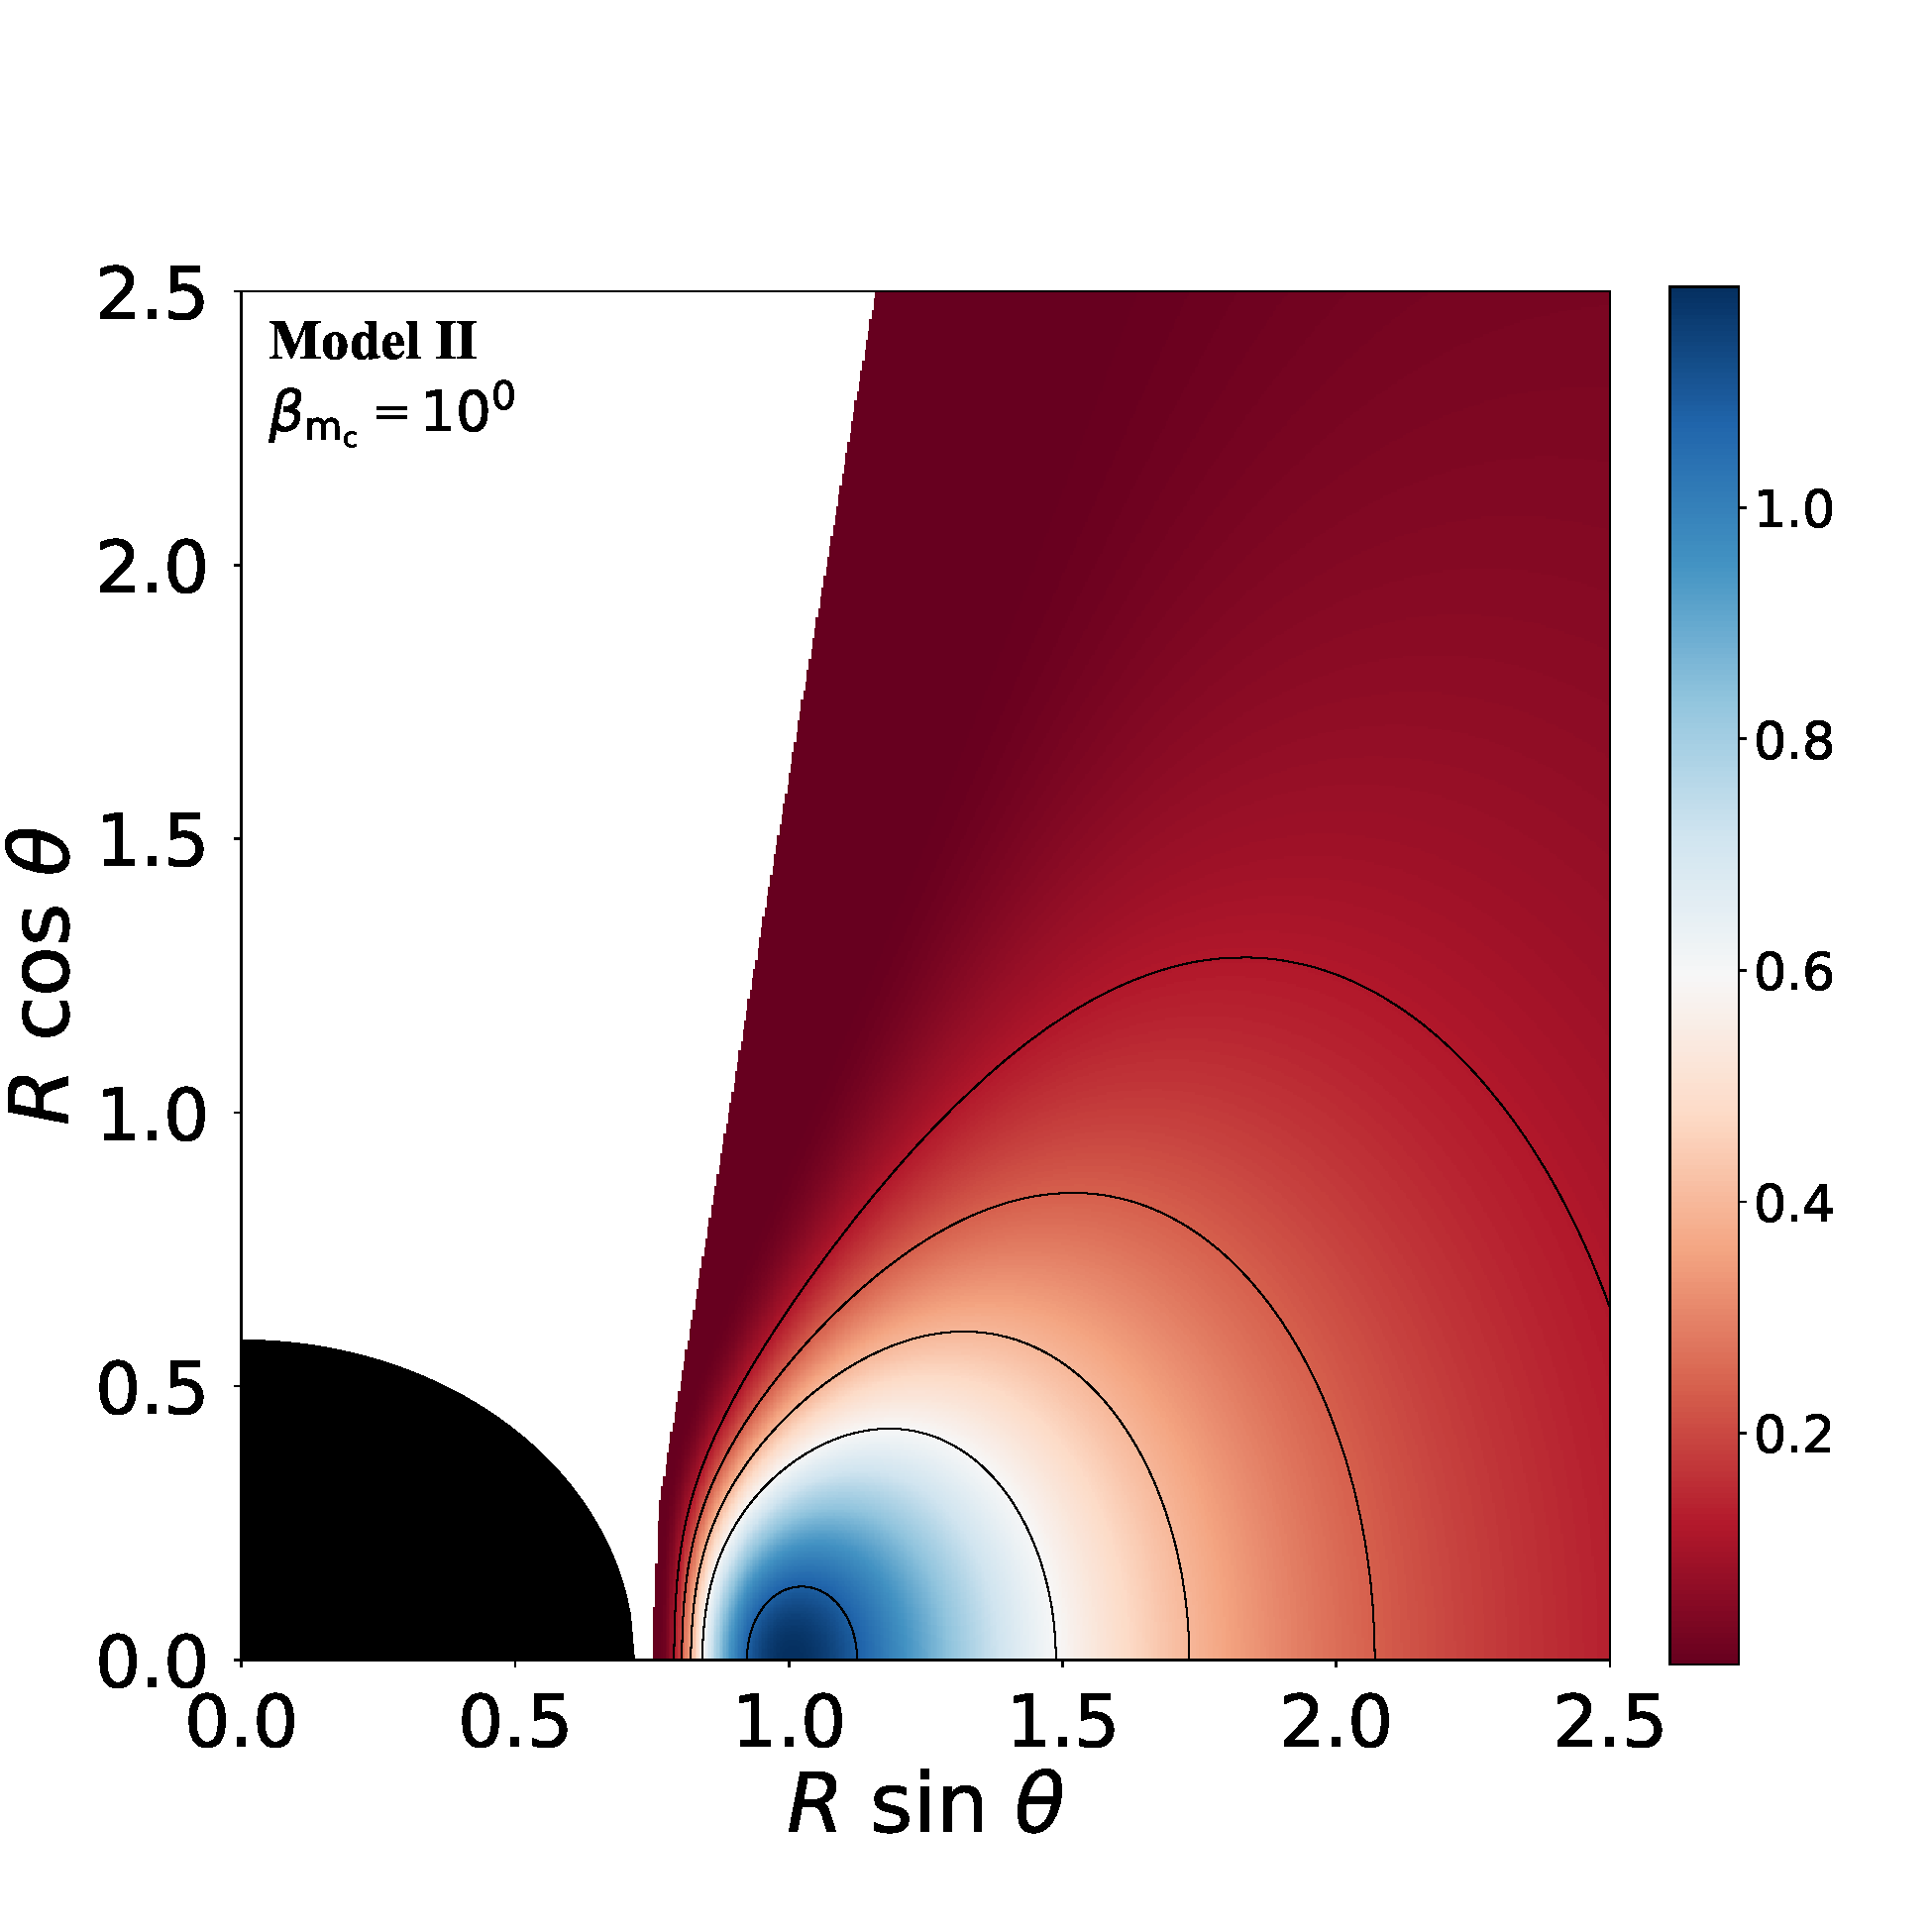
\includegraphics[scale=0.14]{figures/fig3_II_1.pdf}
\hspace{-0.2cm}
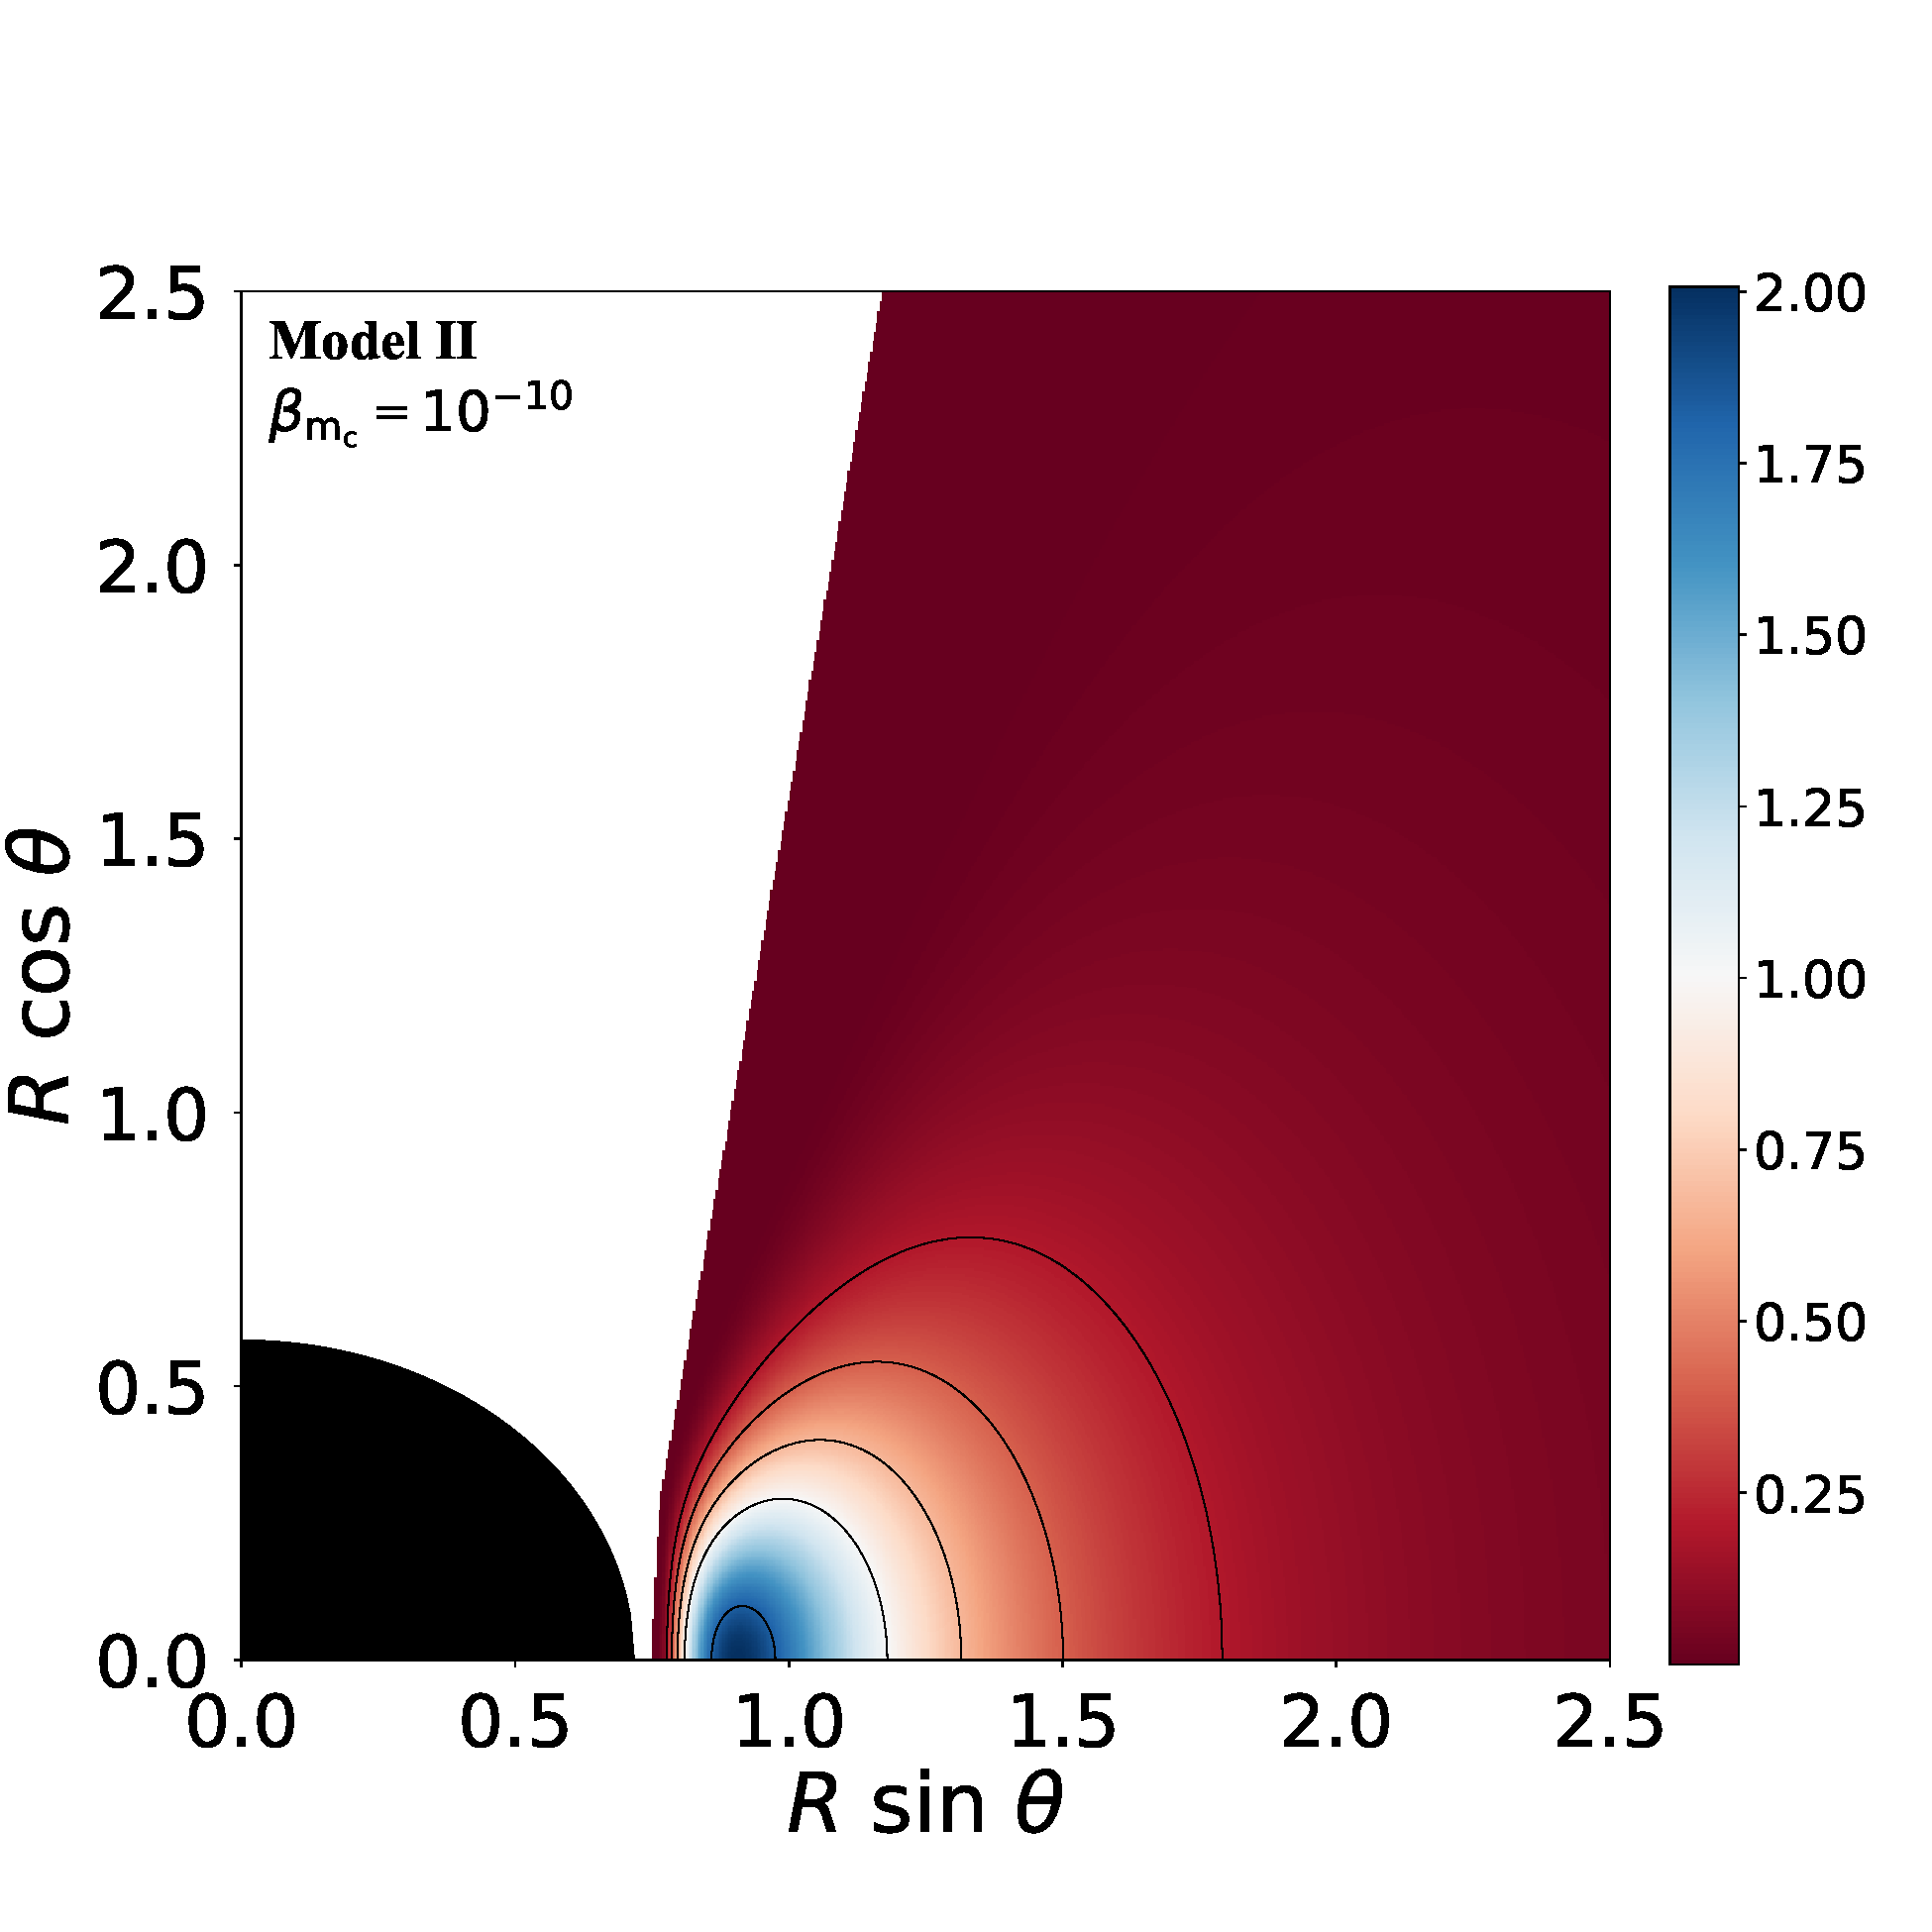
\includegraphics[scale=0.14]{figures/fig3_II__10.pdf}
\\
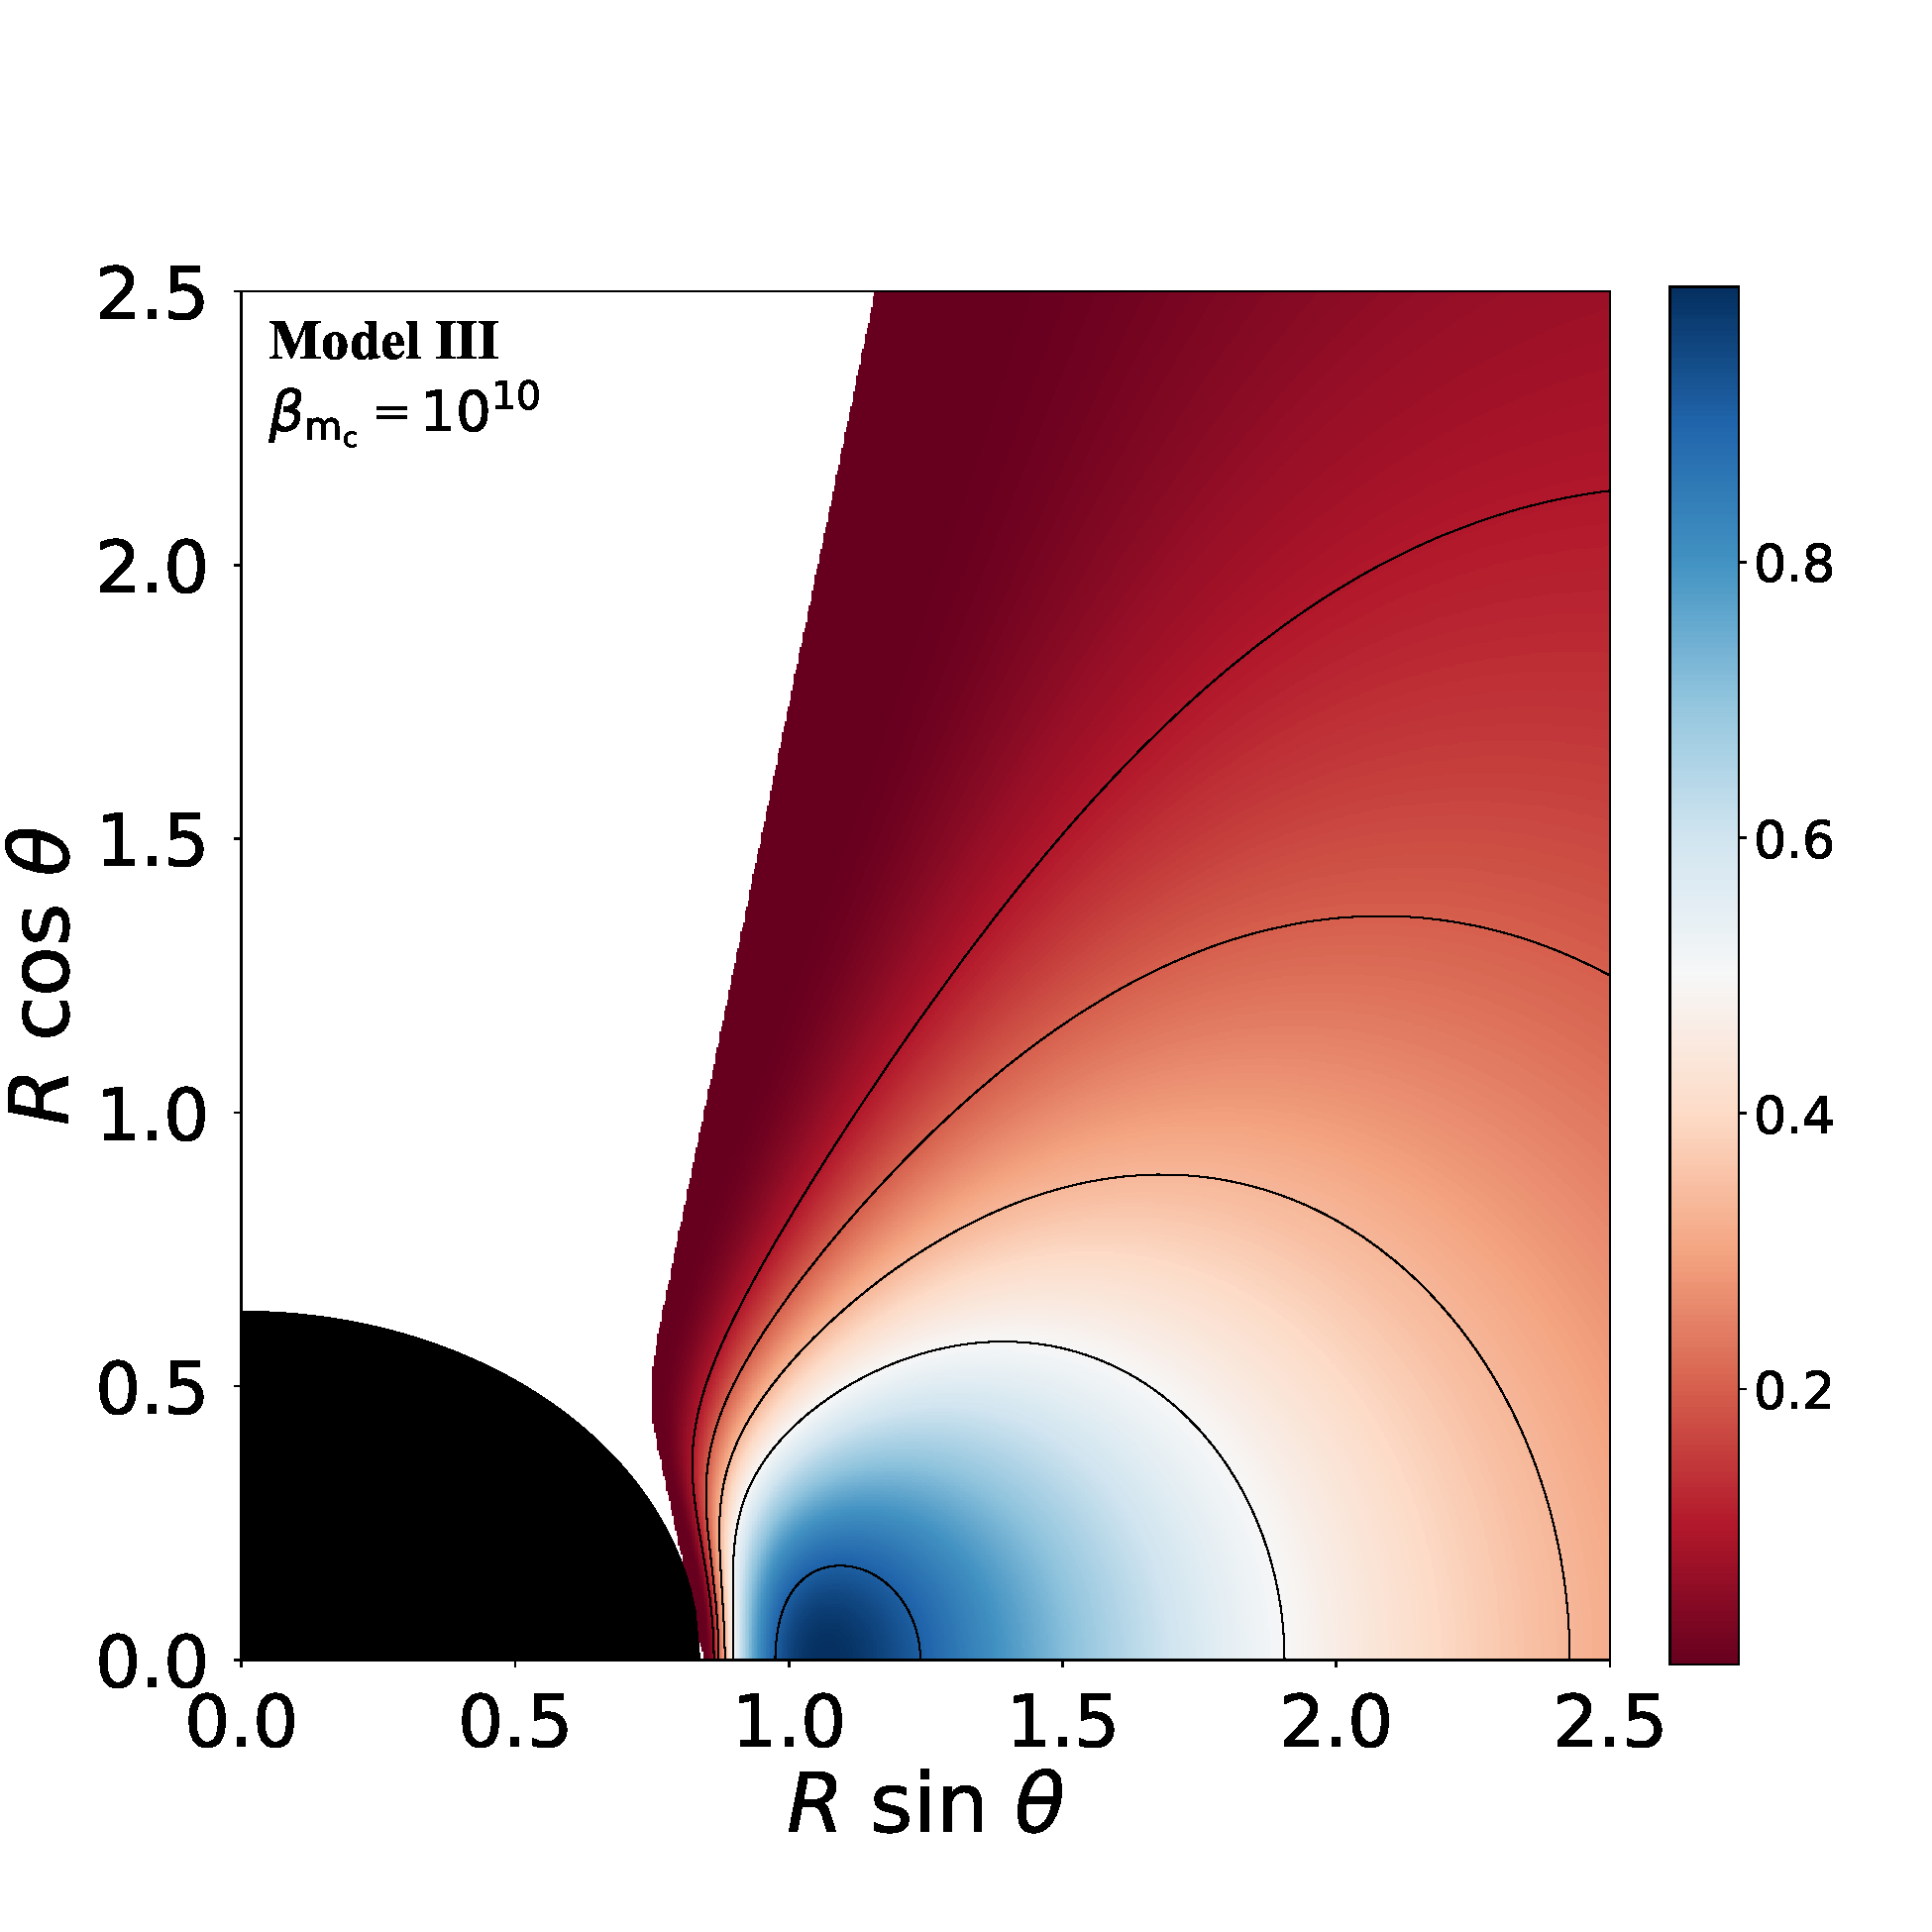
\includegraphics[scale=0.14]{figures/fig3_III_10.pdf}
\hspace{-0.3cm}
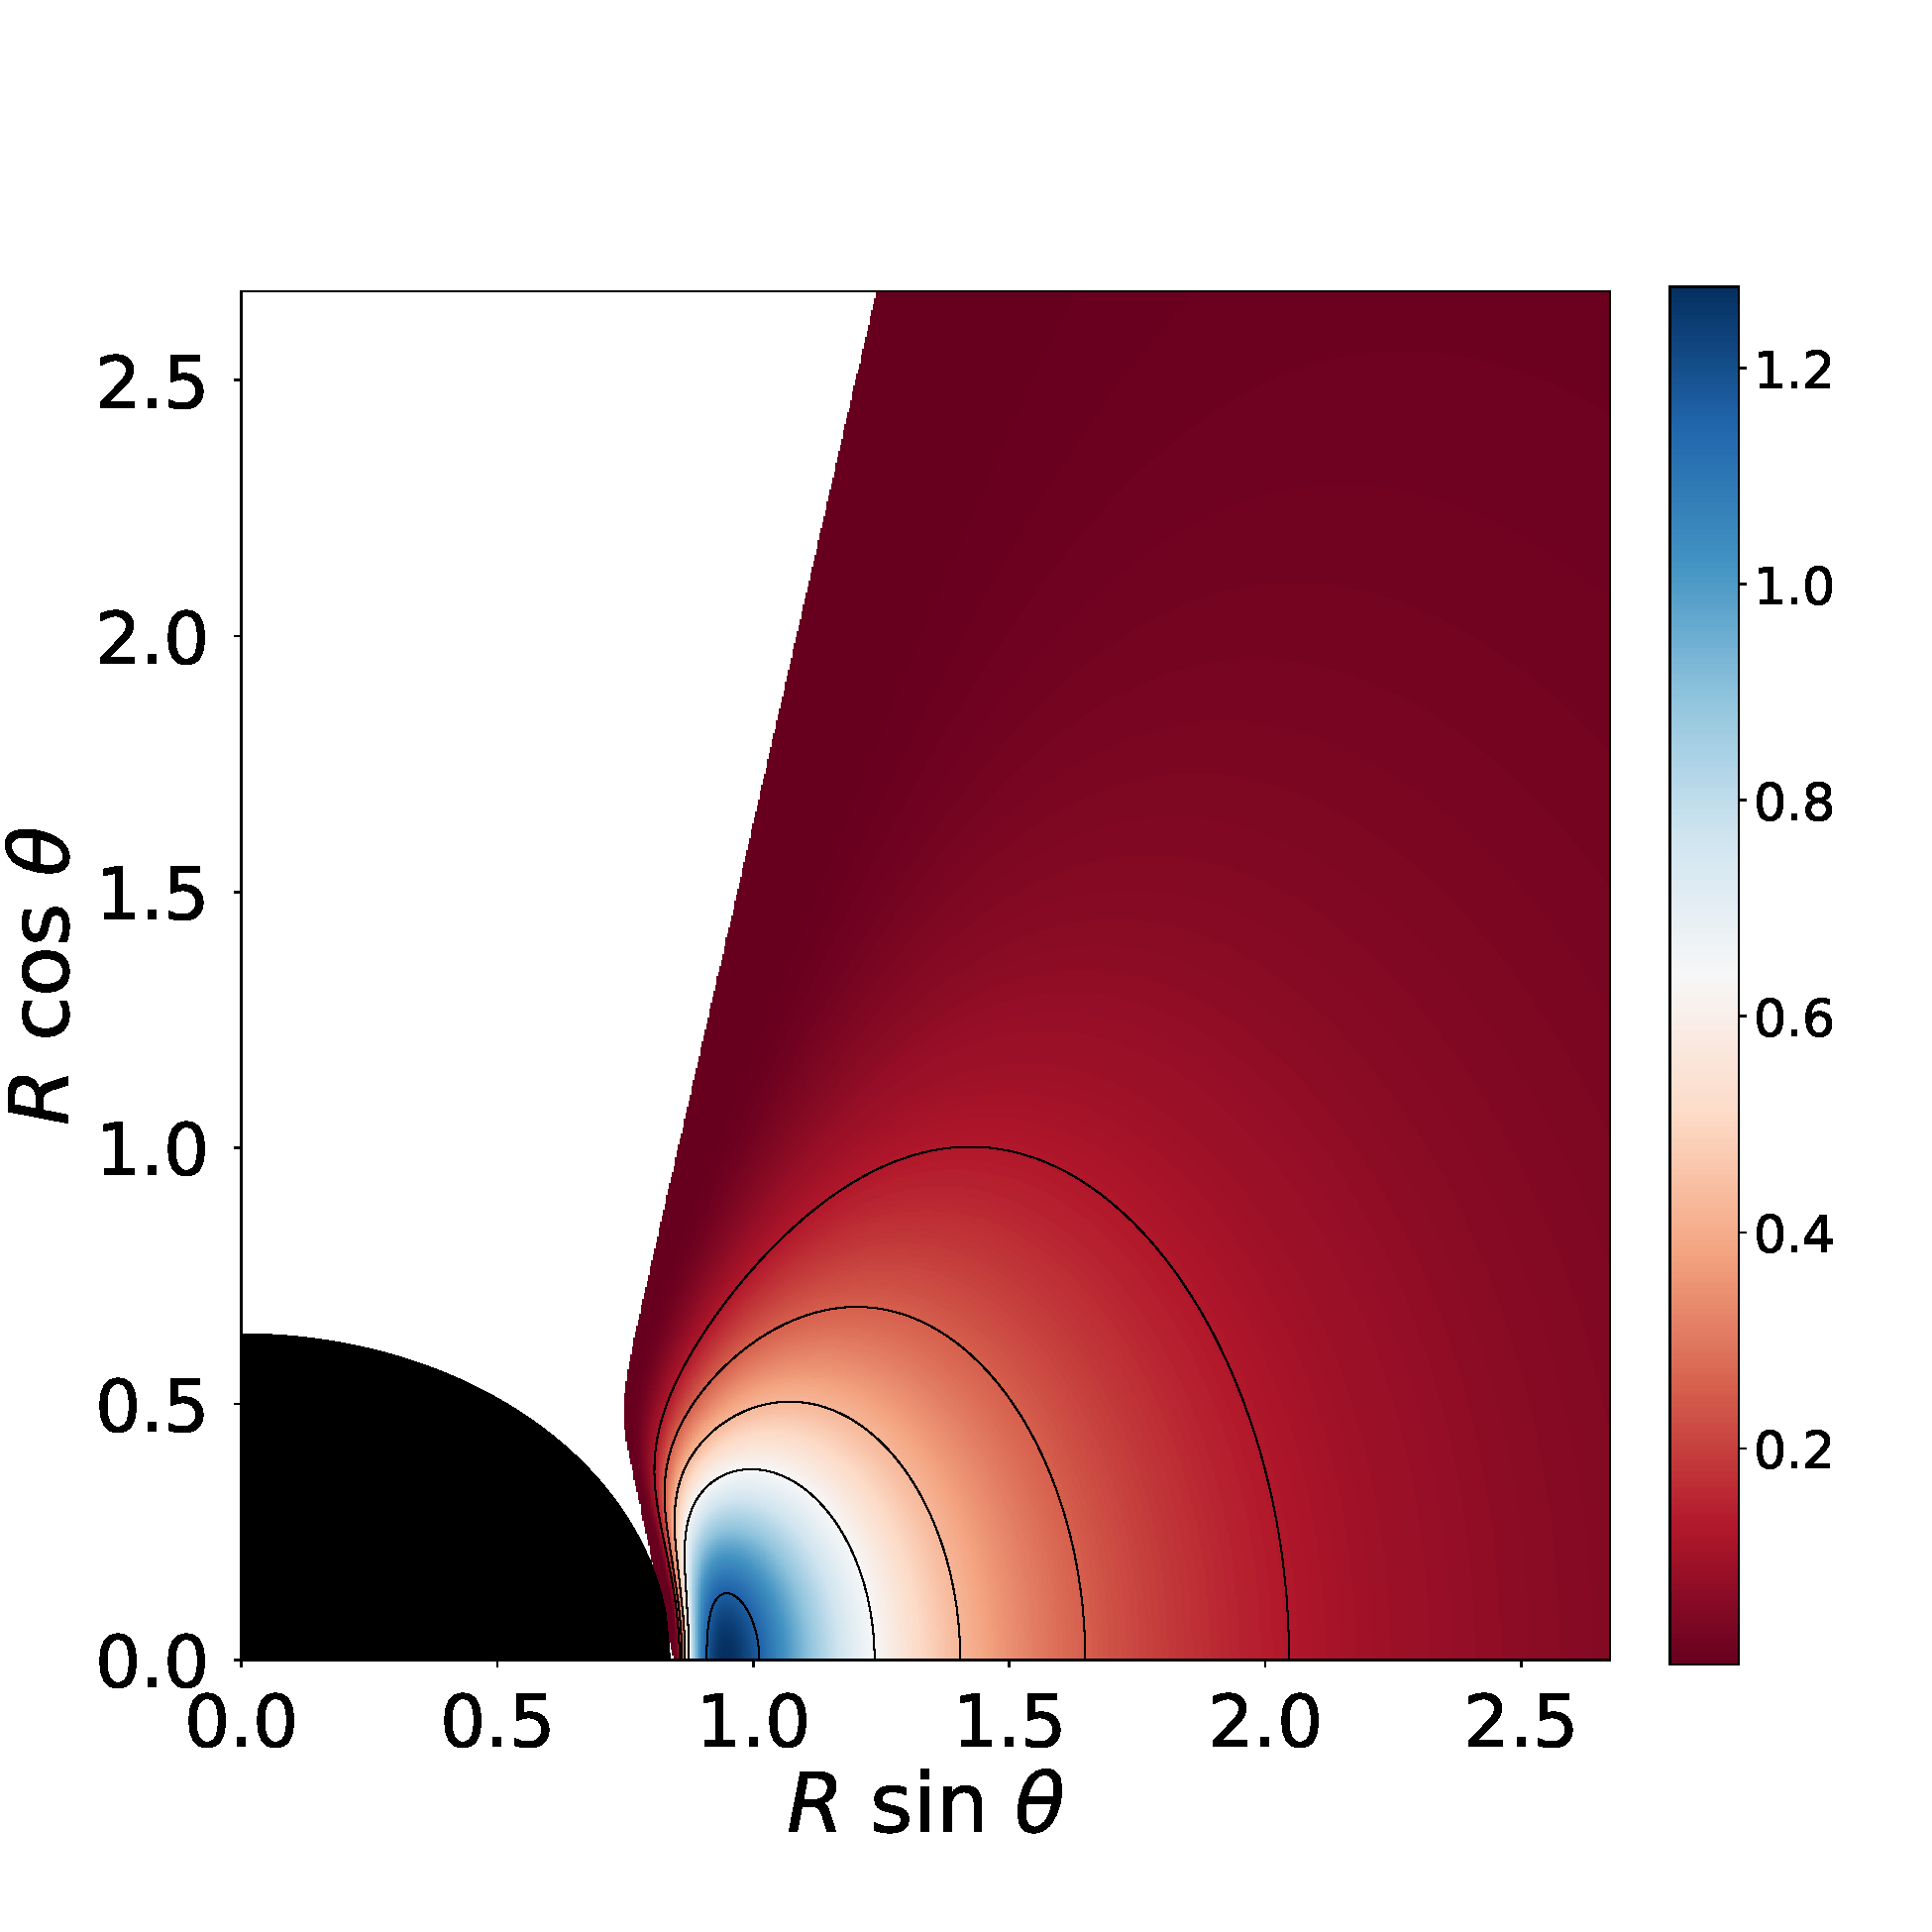
\includegraphics[scale=0.14]{figures/fig3_III_1.pdf}
\hspace{-0.2cm}
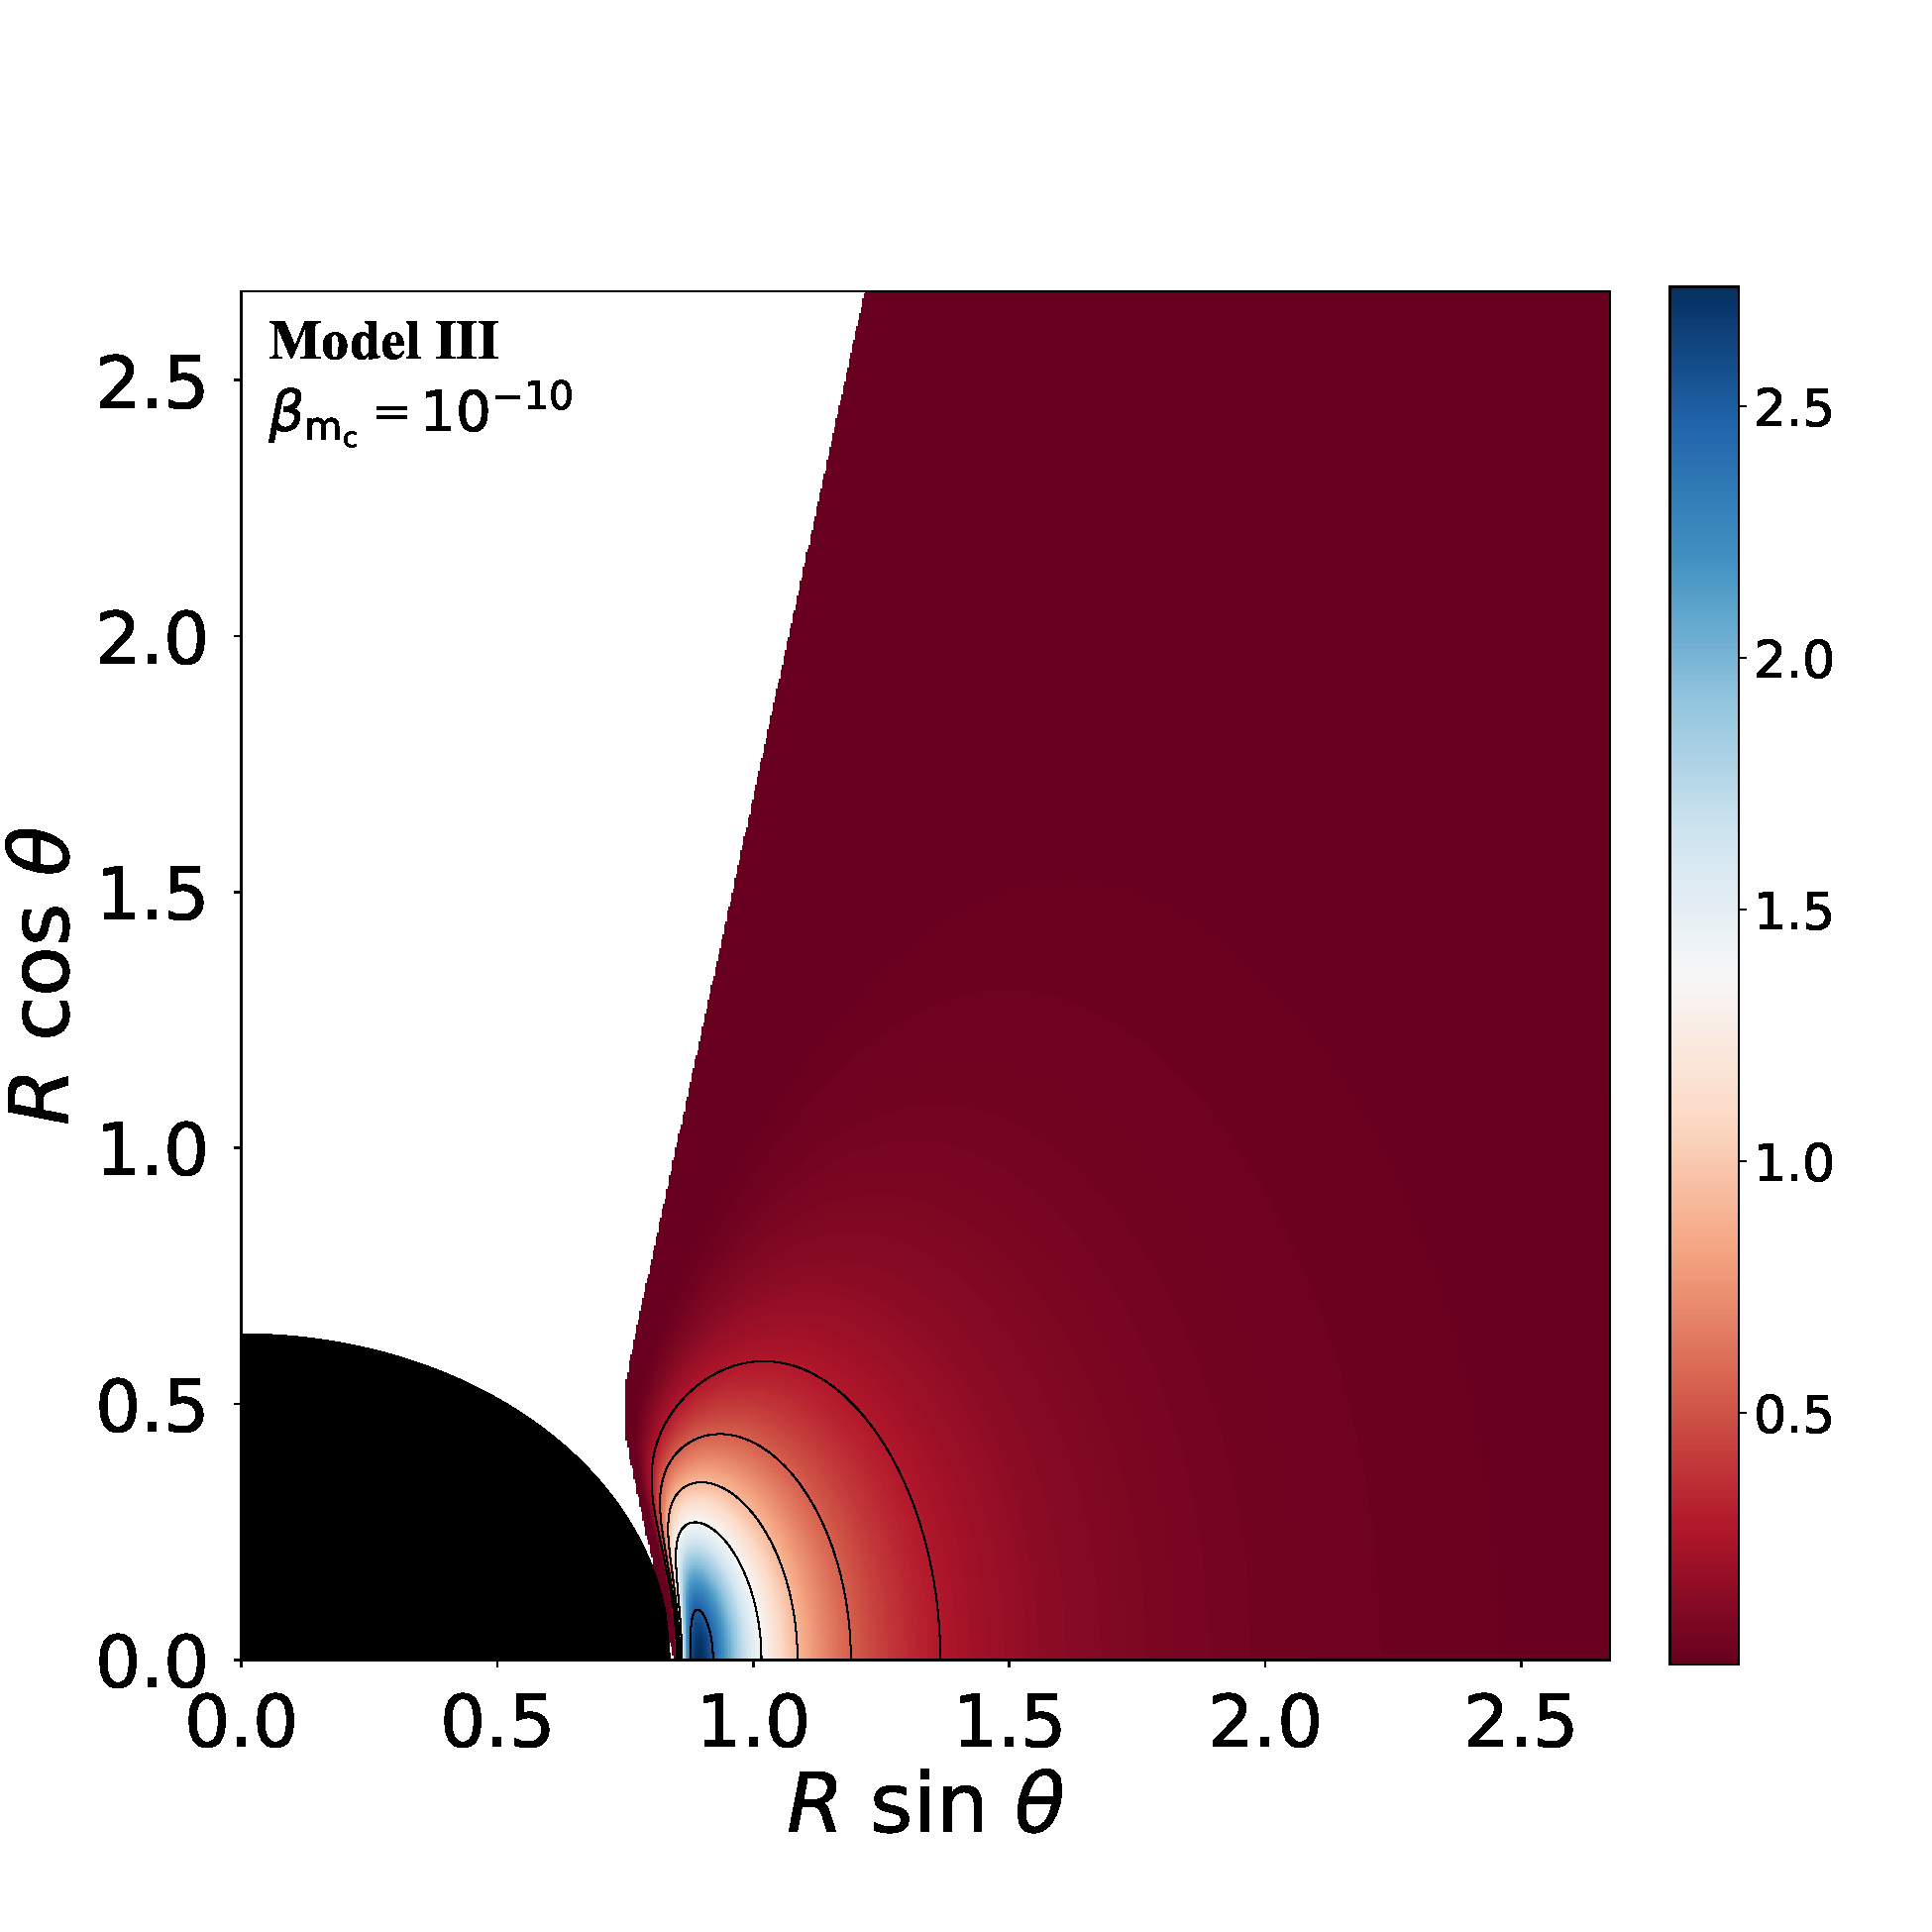
\includegraphics[scale=0.14]{figures/fig3_III__10.pdf}
\\
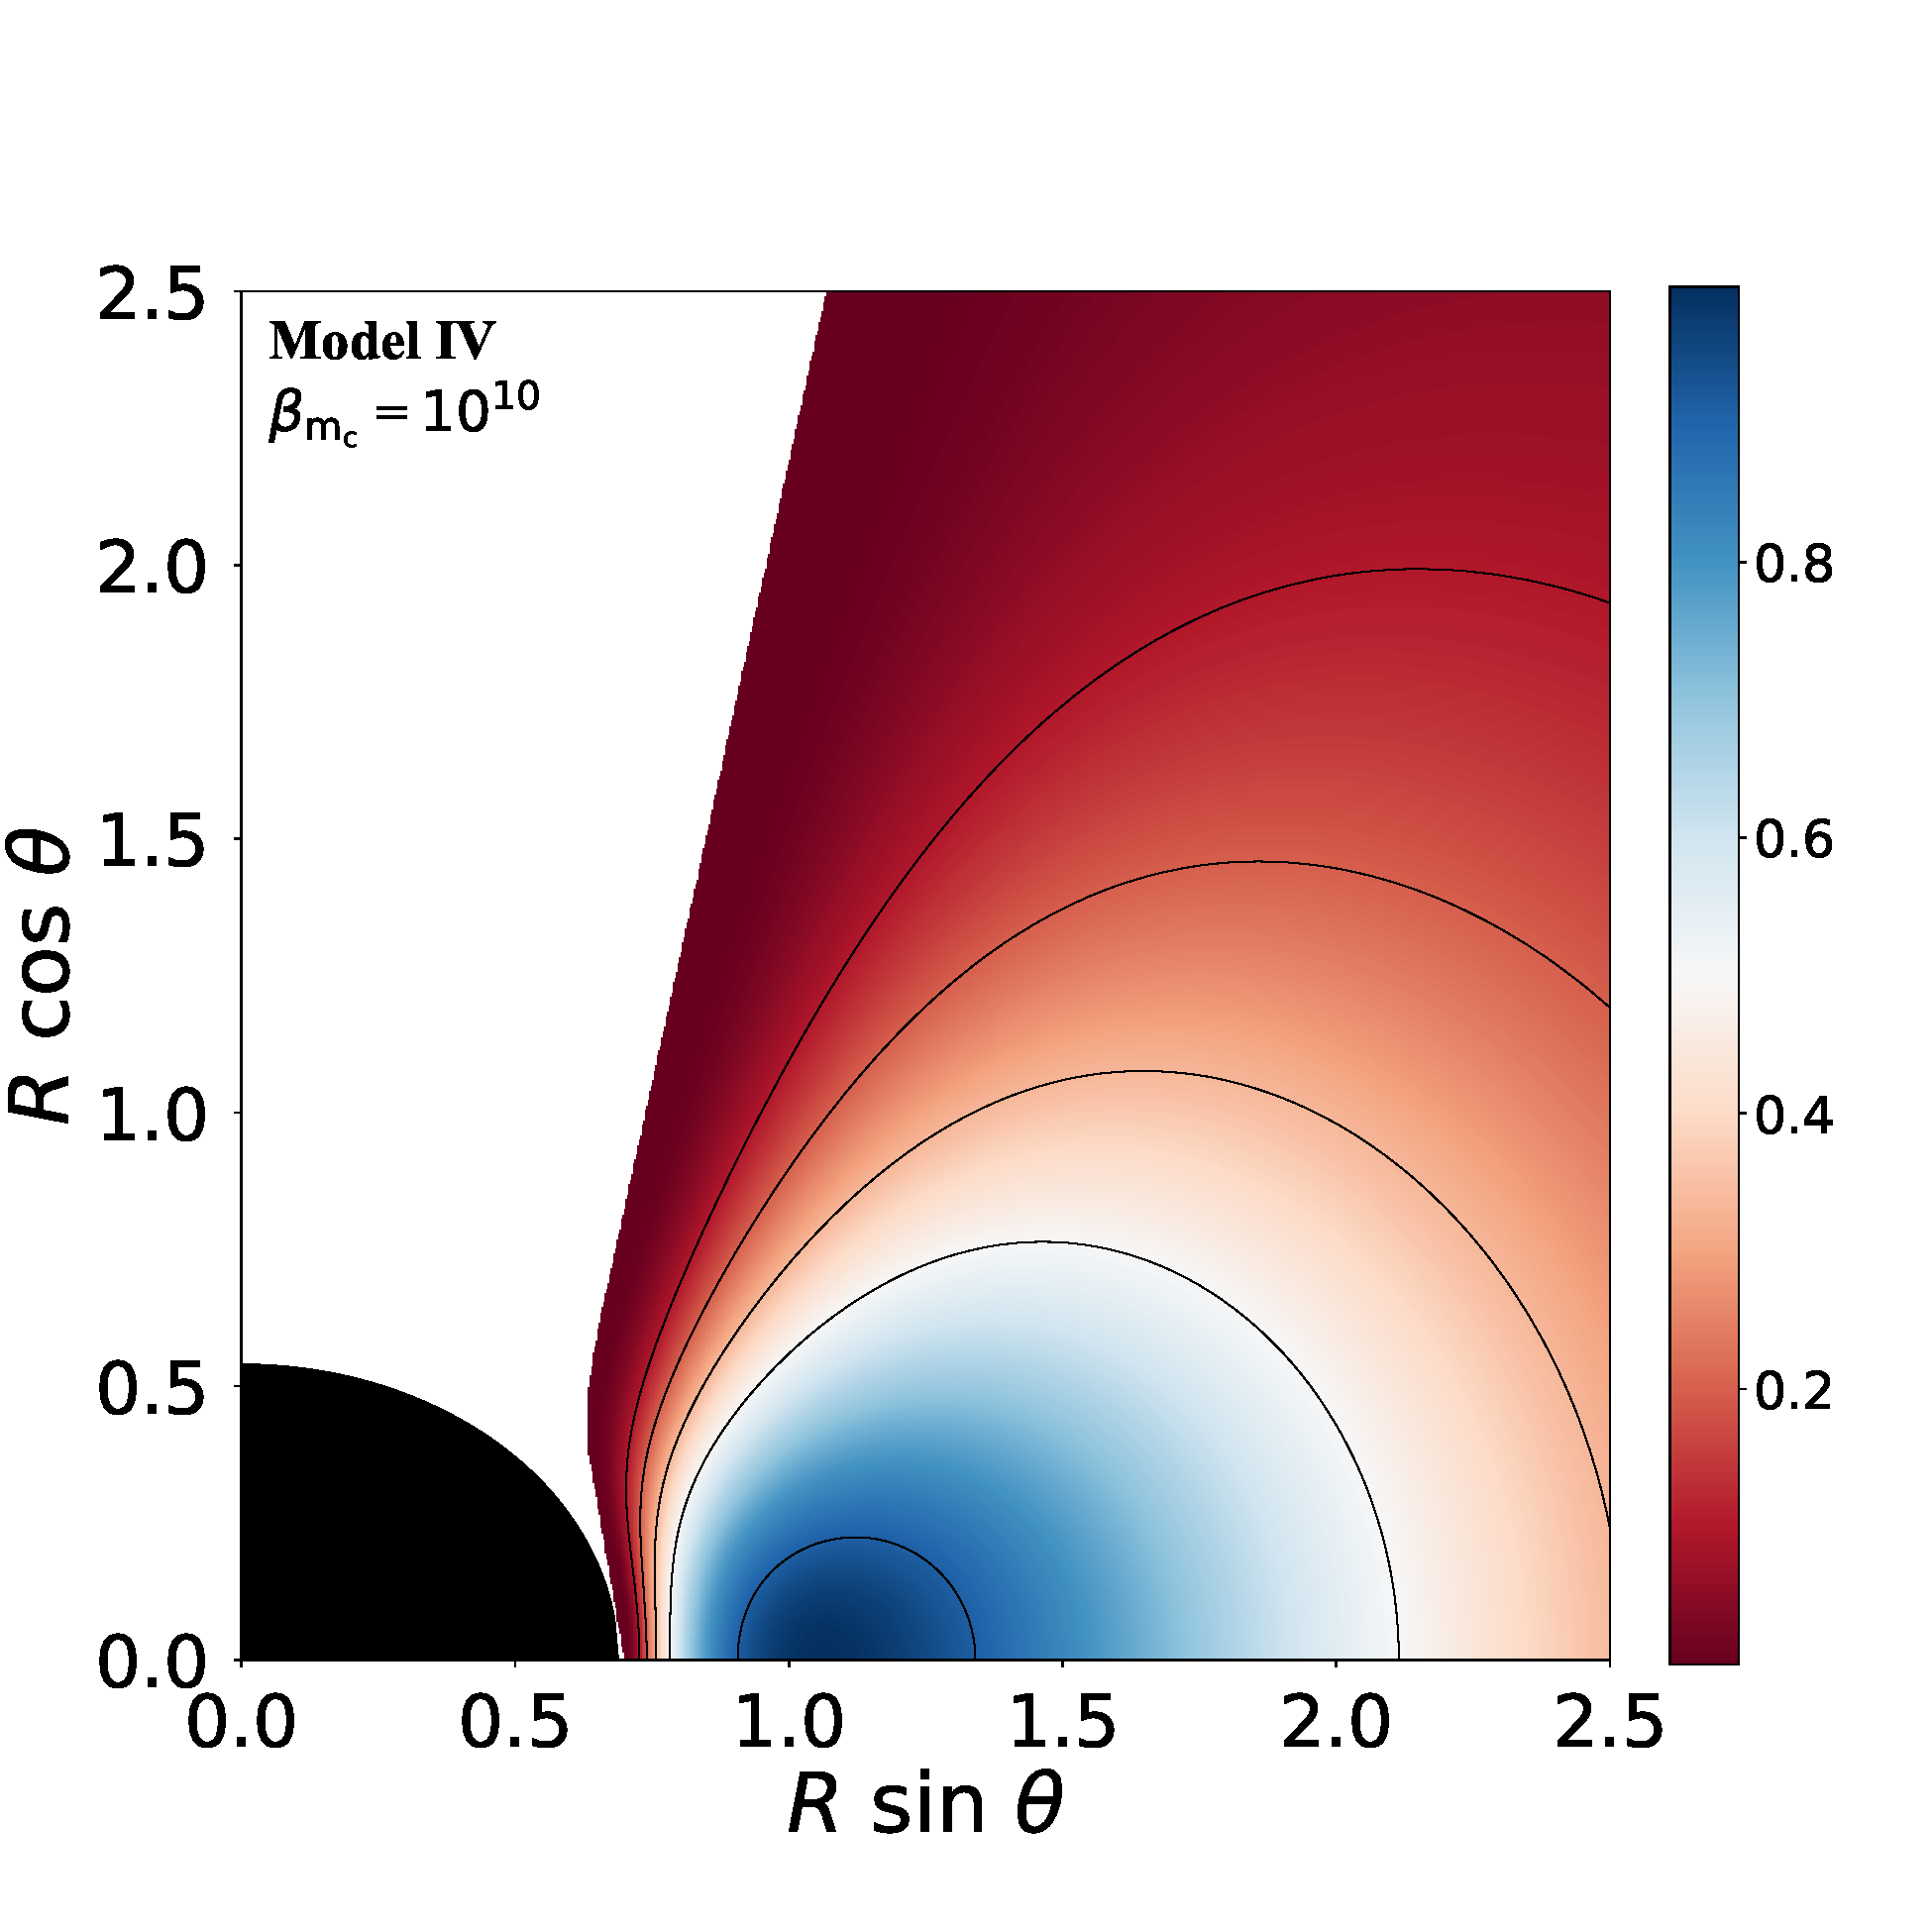
\includegraphics[scale=0.14]{figures/fig3_IV_10.pdf}
\hspace{-0.3cm}
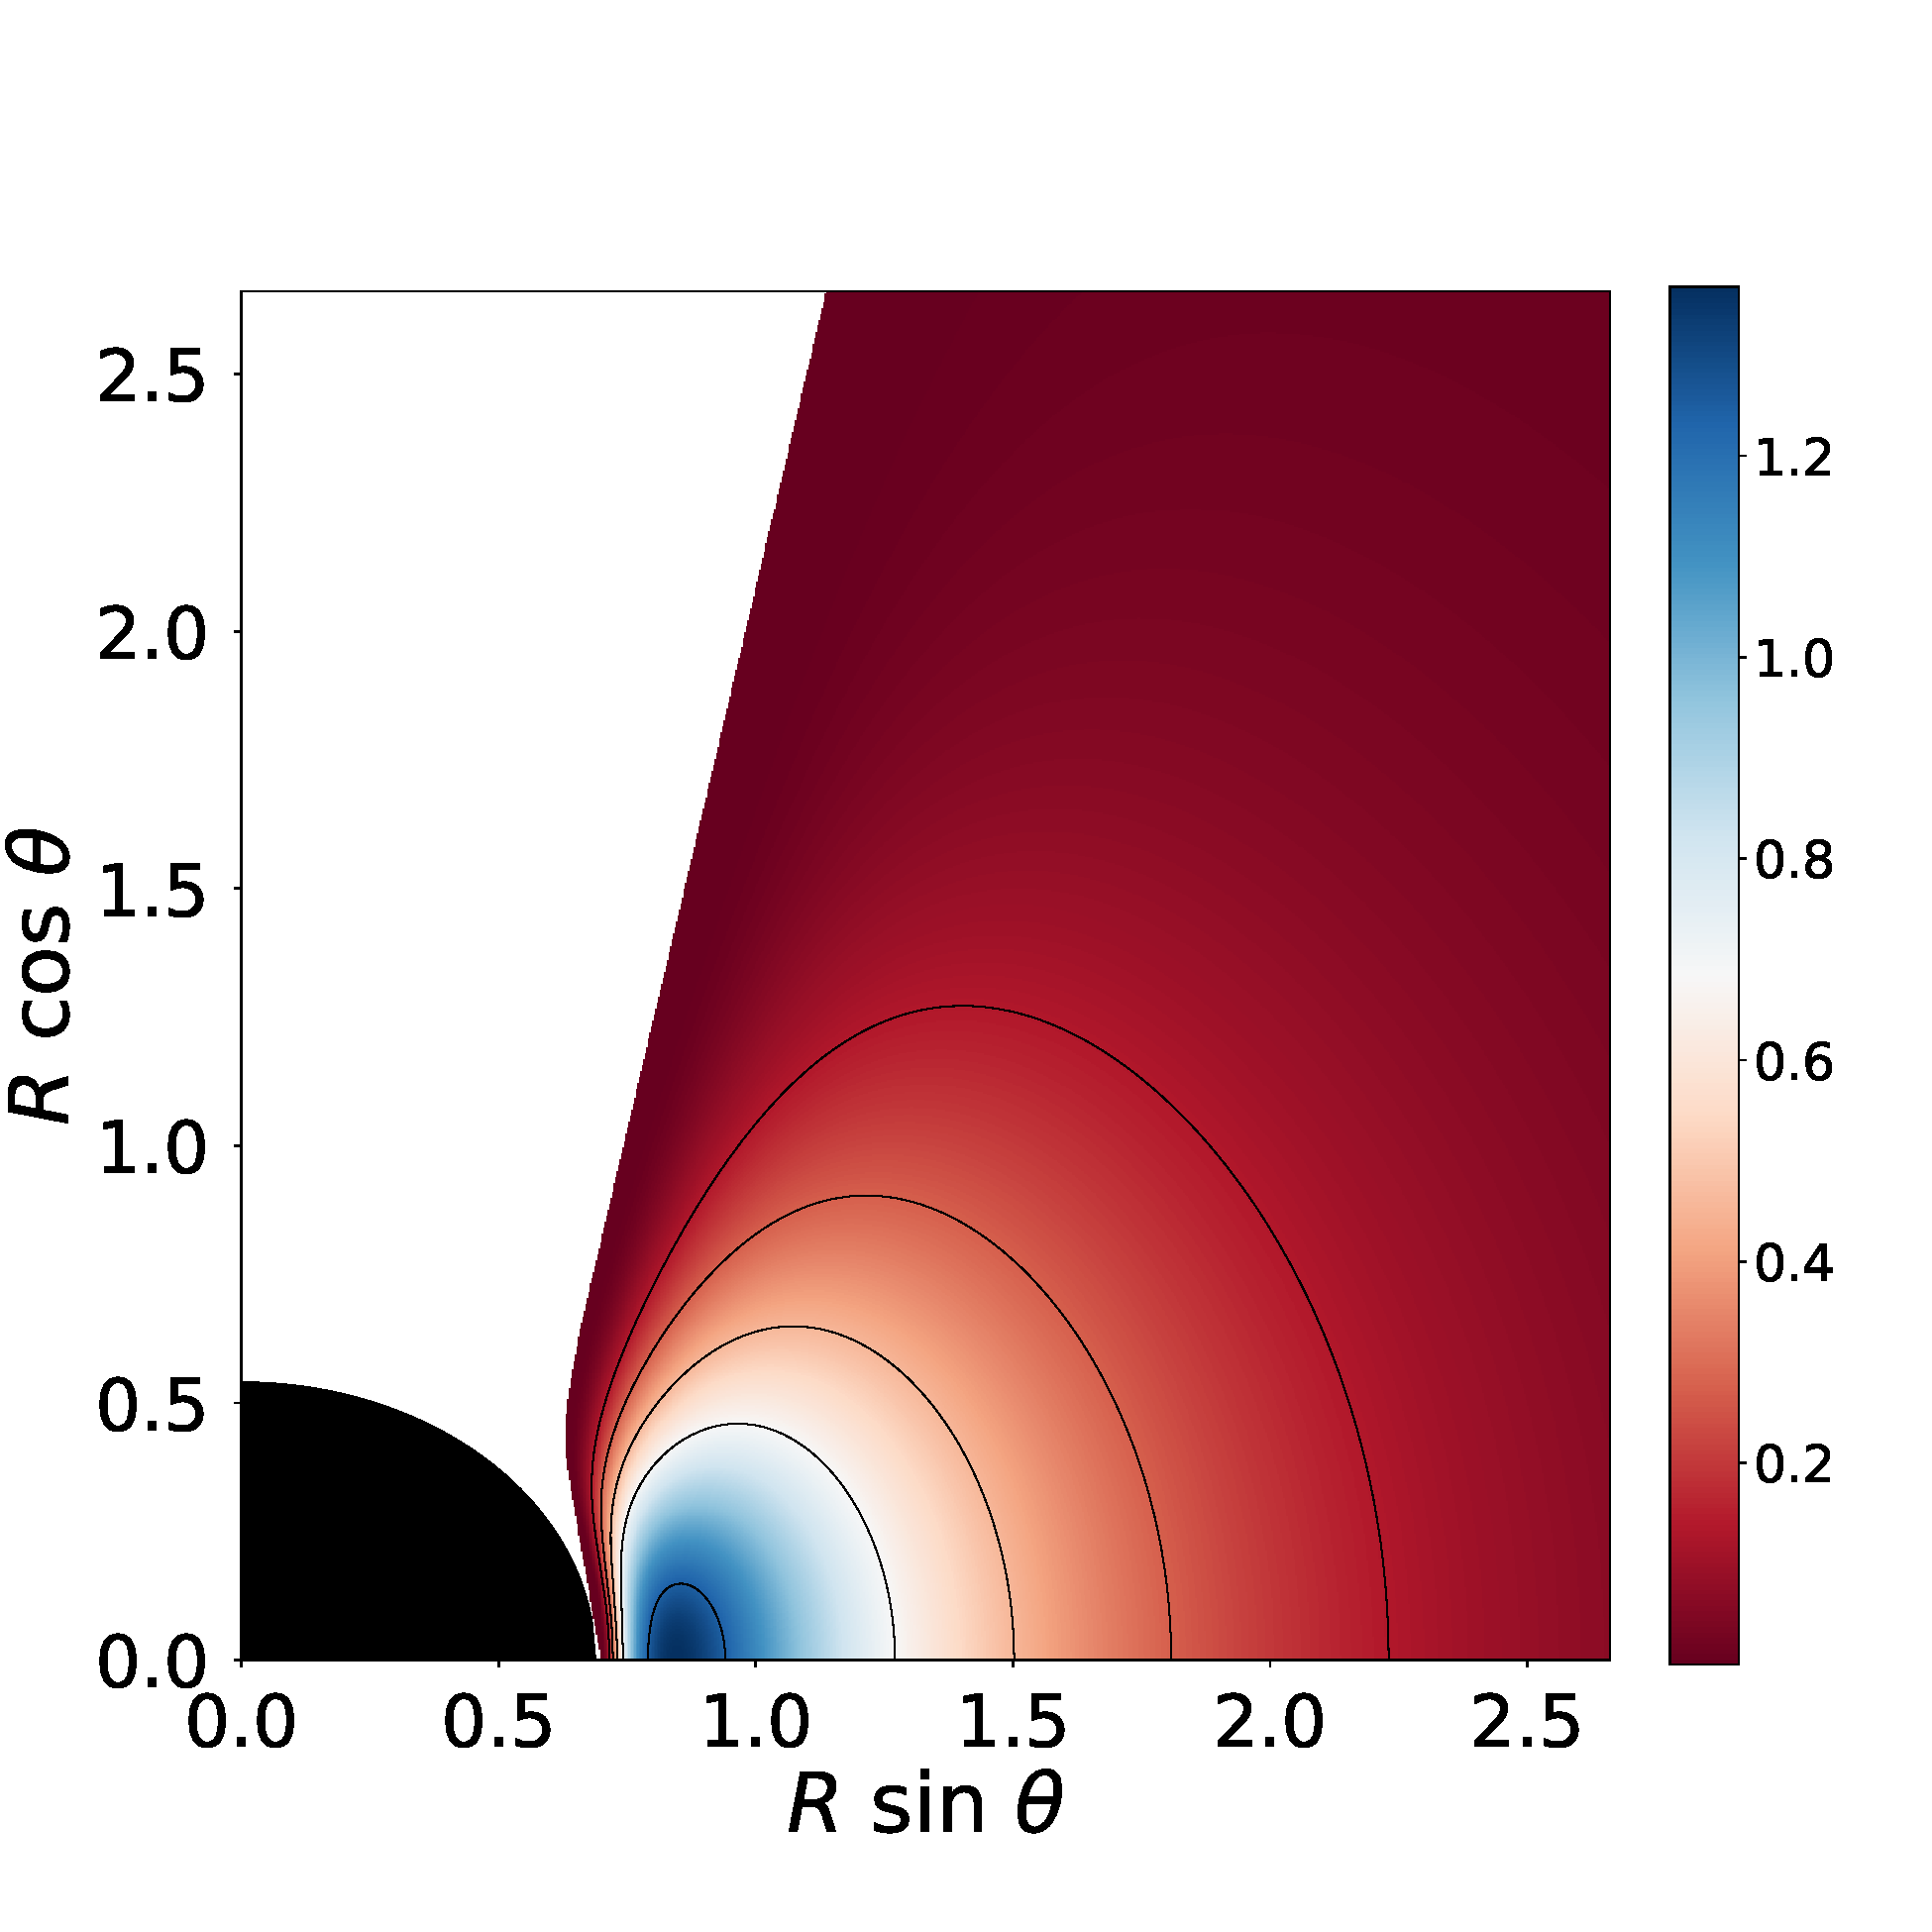
\includegraphics[scale=0.14]{figures/fig3_IV_1.pdf}
\hspace{-0.2cm}
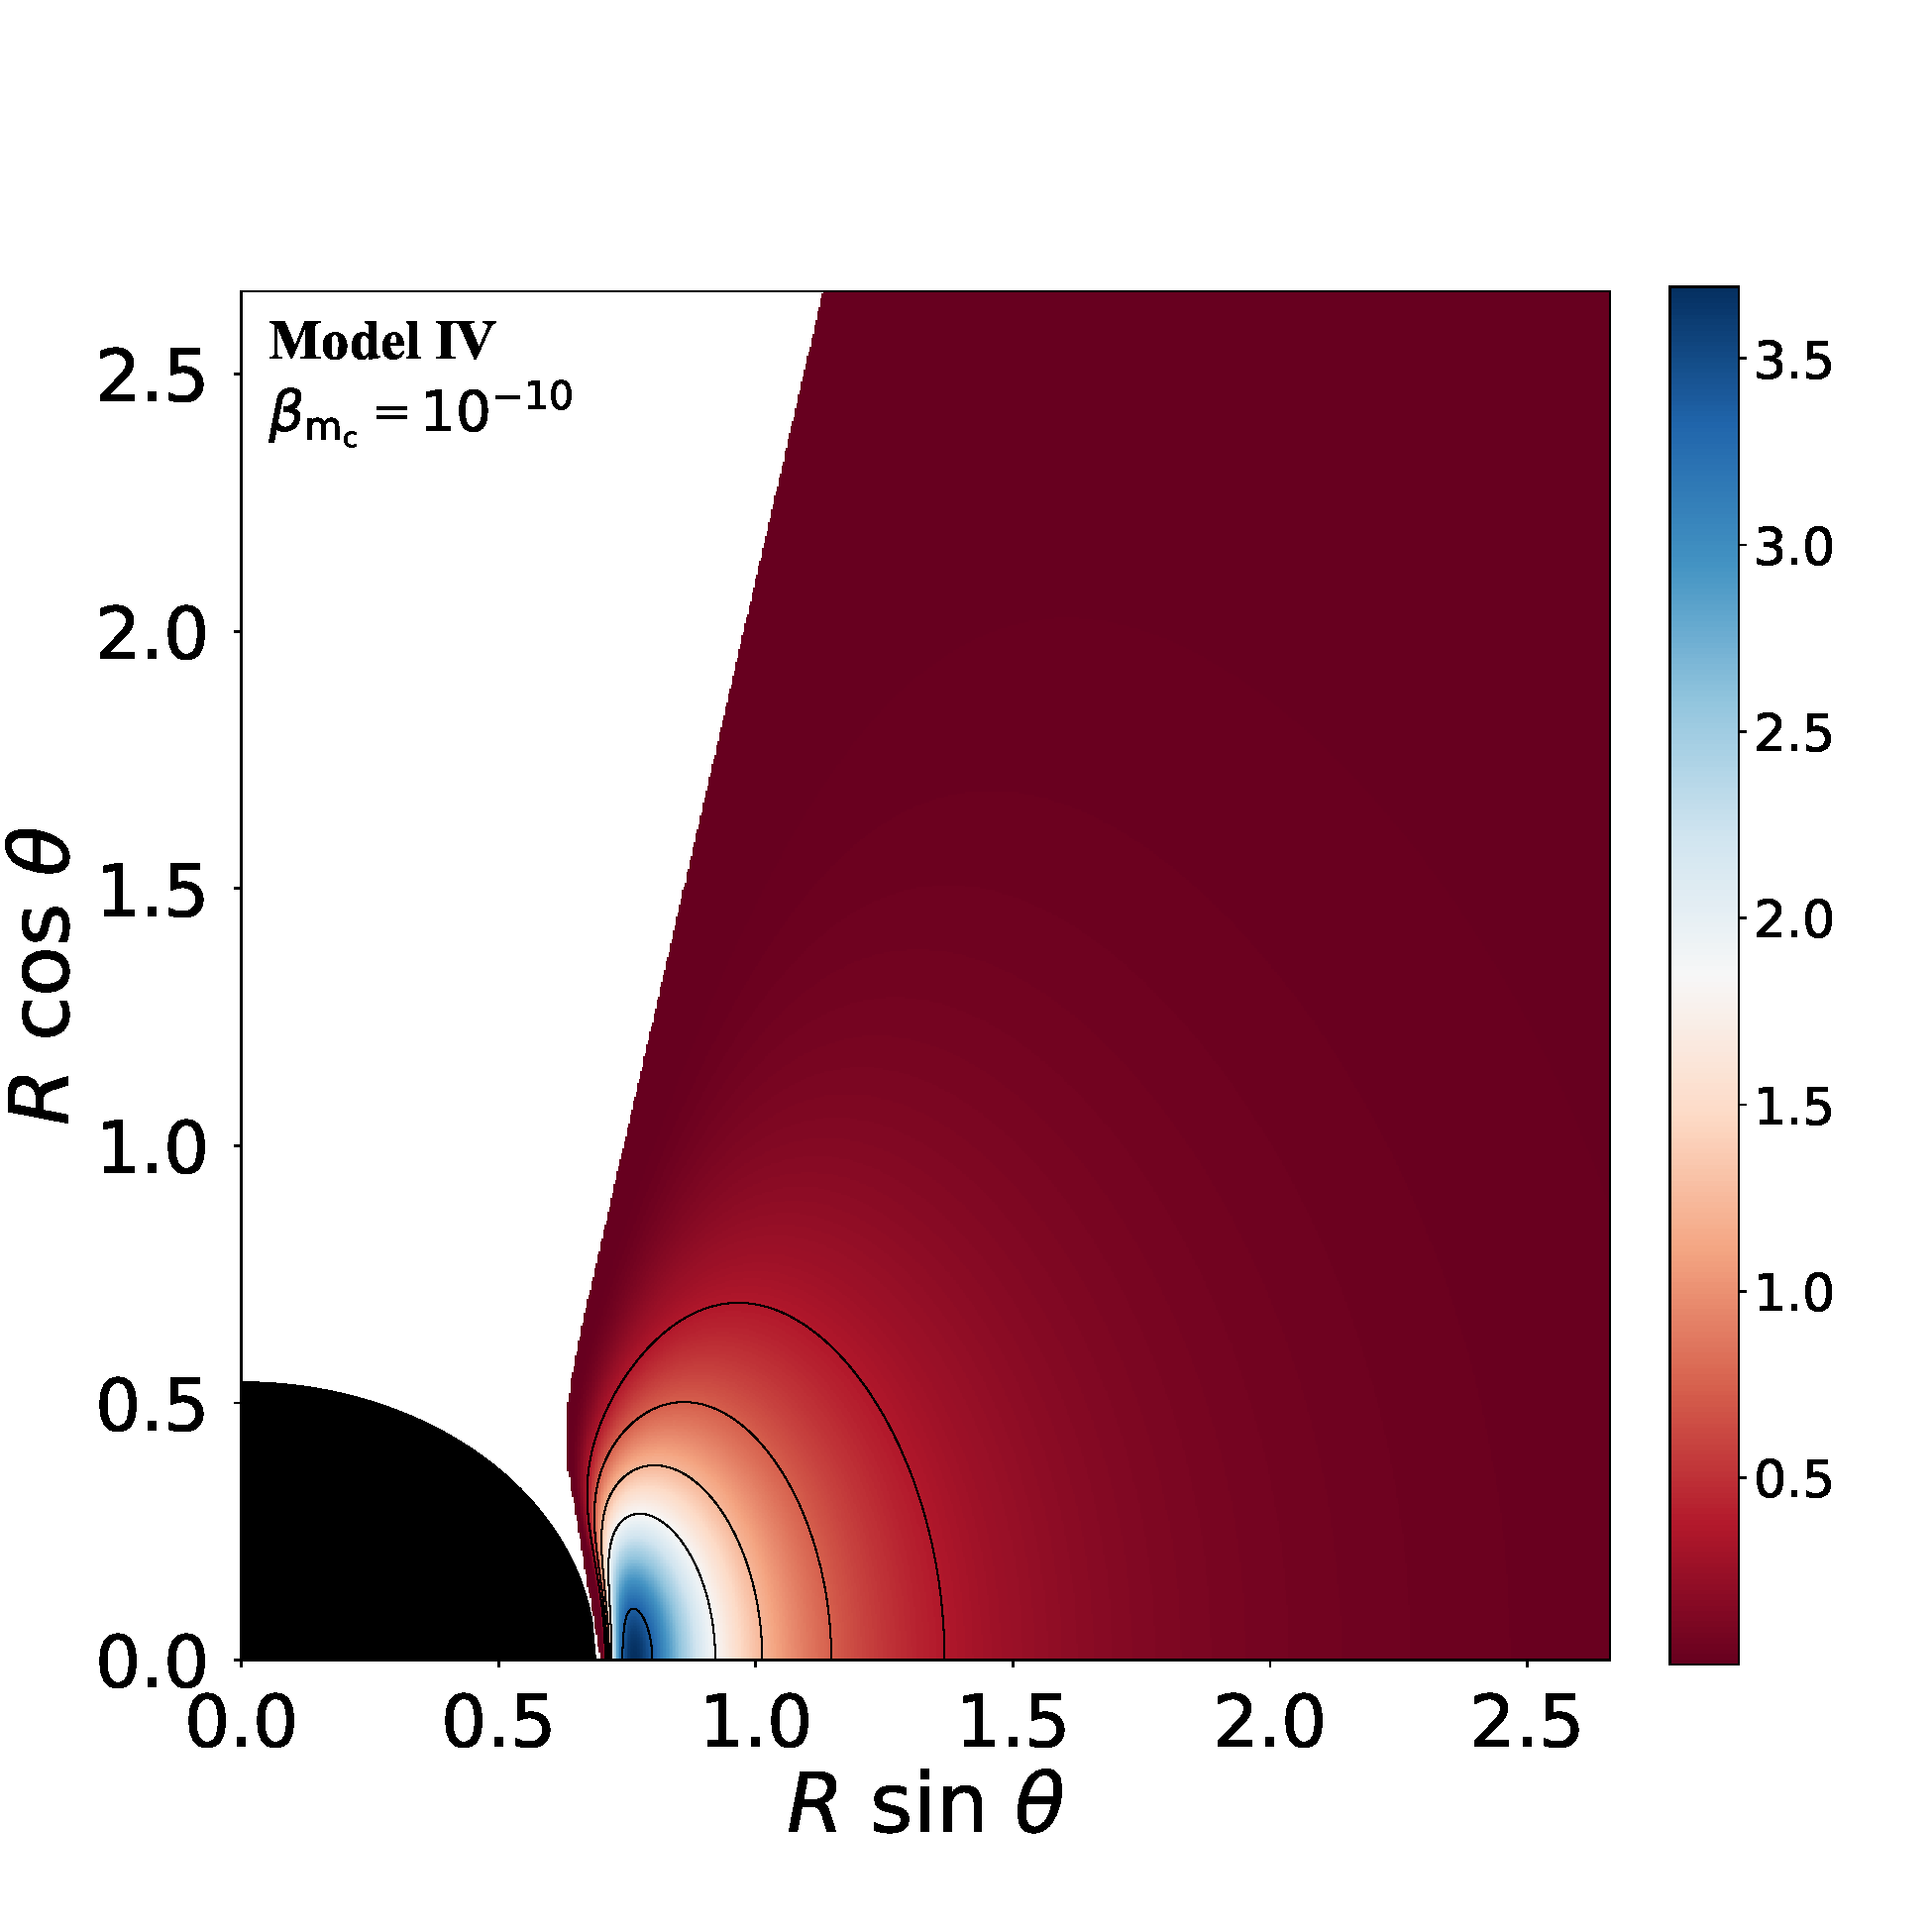
\includegraphics[scale=0.14]{figures/fig3_IV__10.pdf}
\hspace{-0.2cm}
\caption{Same as Fig.~\ref{models_I} but using the perimetral radial coordinate $R$. \tf{Same comment as in the previous figure.}}
\label{models_peri_I}
\end{figure*}

\begin{figure*}
\centering
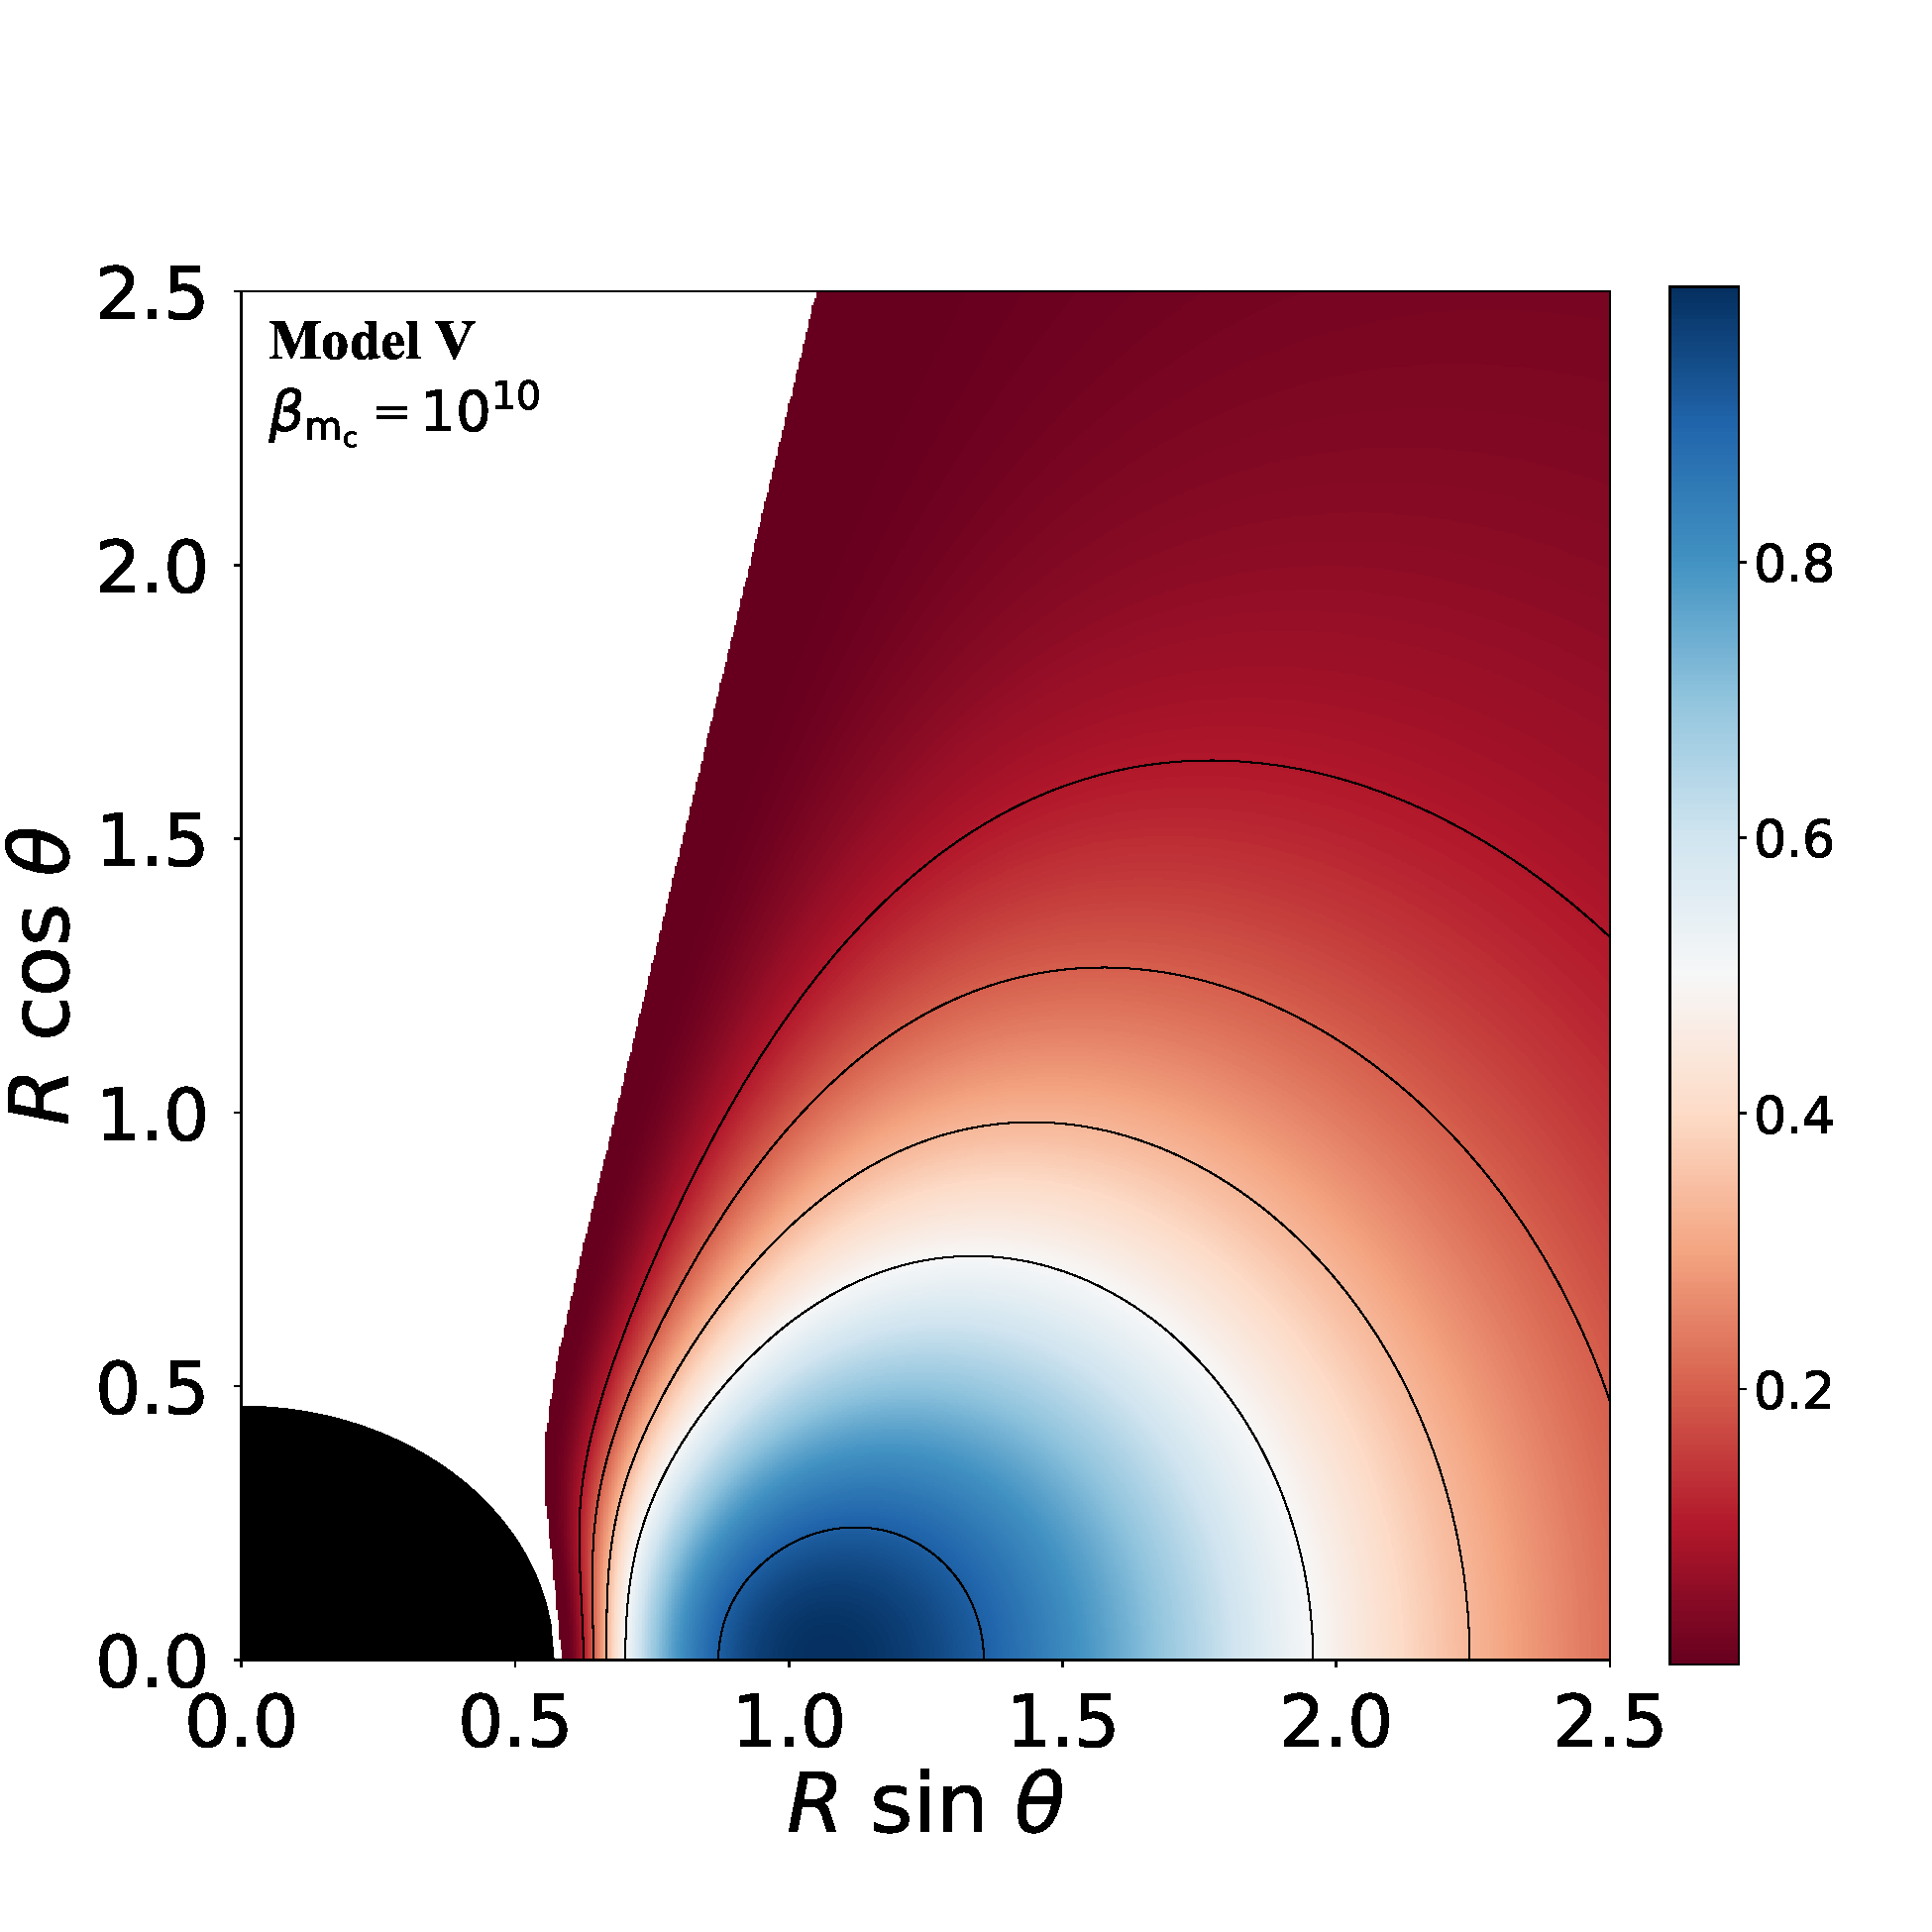
\includegraphics[scale=0.14]{figures/fig4_V_10.pdf}
\hspace{-0.3cm}
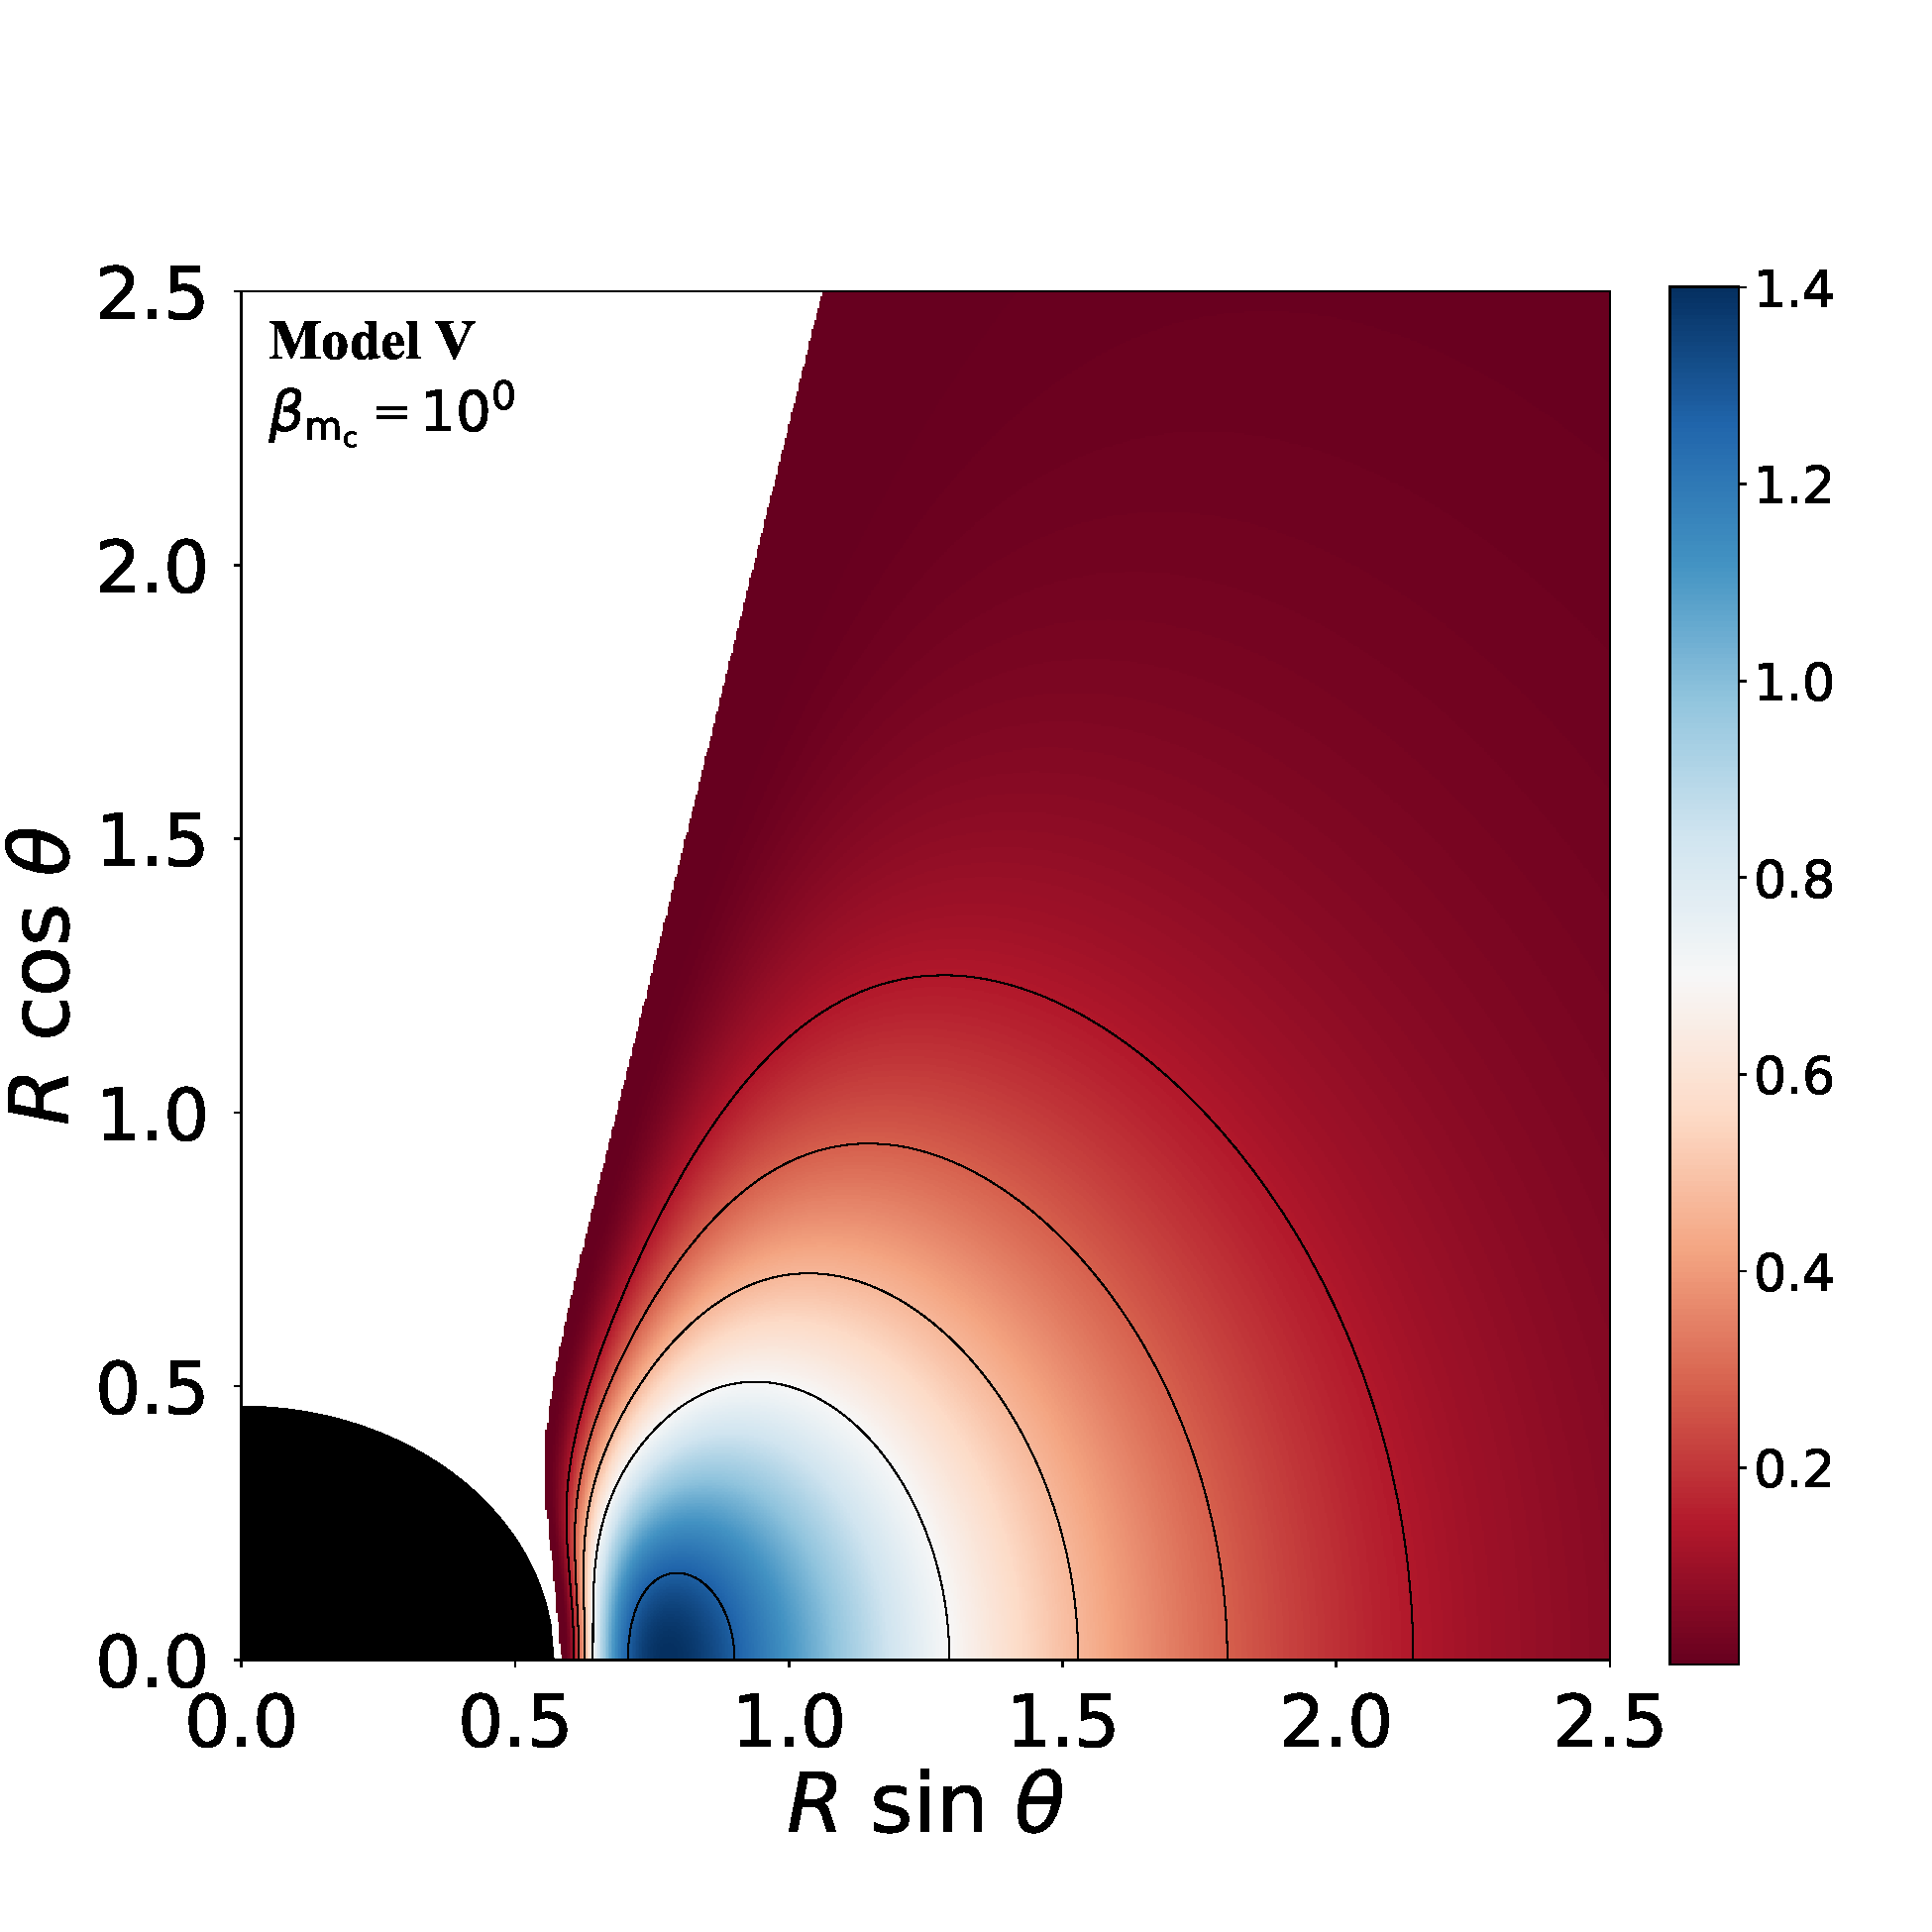
\includegraphics[scale=0.14]{figures/fig4_V_1.pdf}
\hspace{-0.2cm}
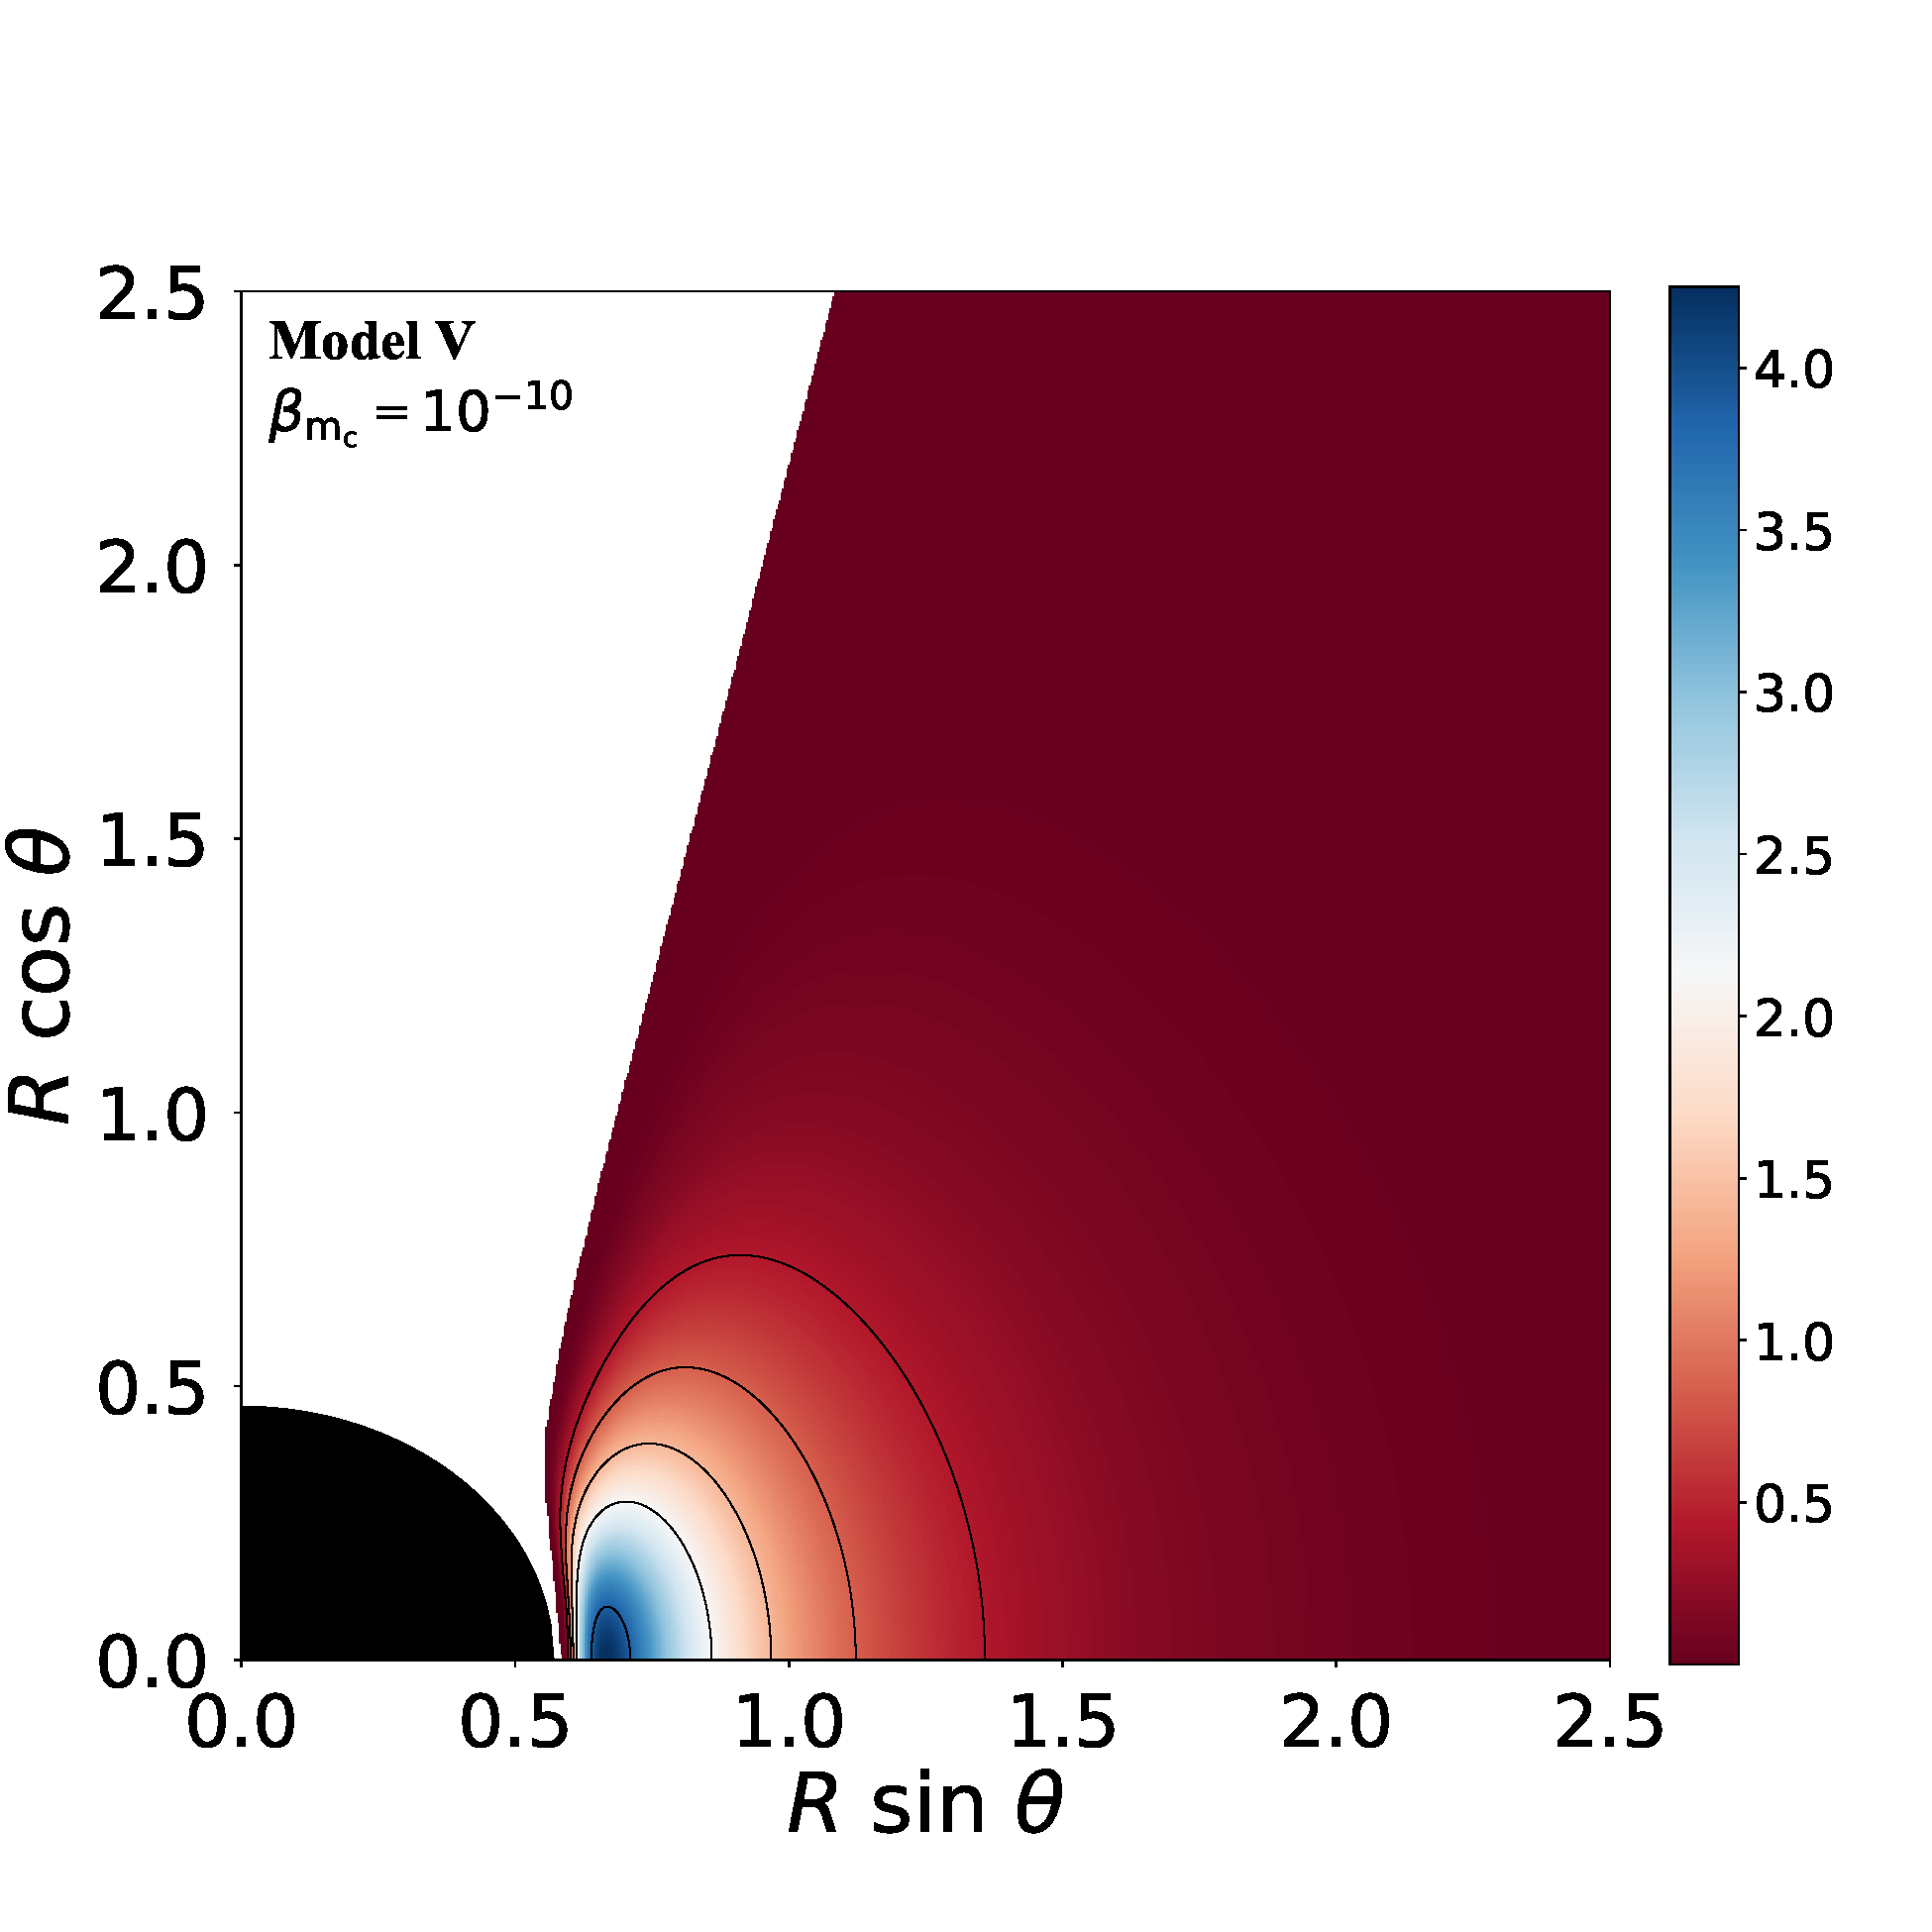
\includegraphics[scale=0.14]{figures/fig4_V__10.pdf}
\\
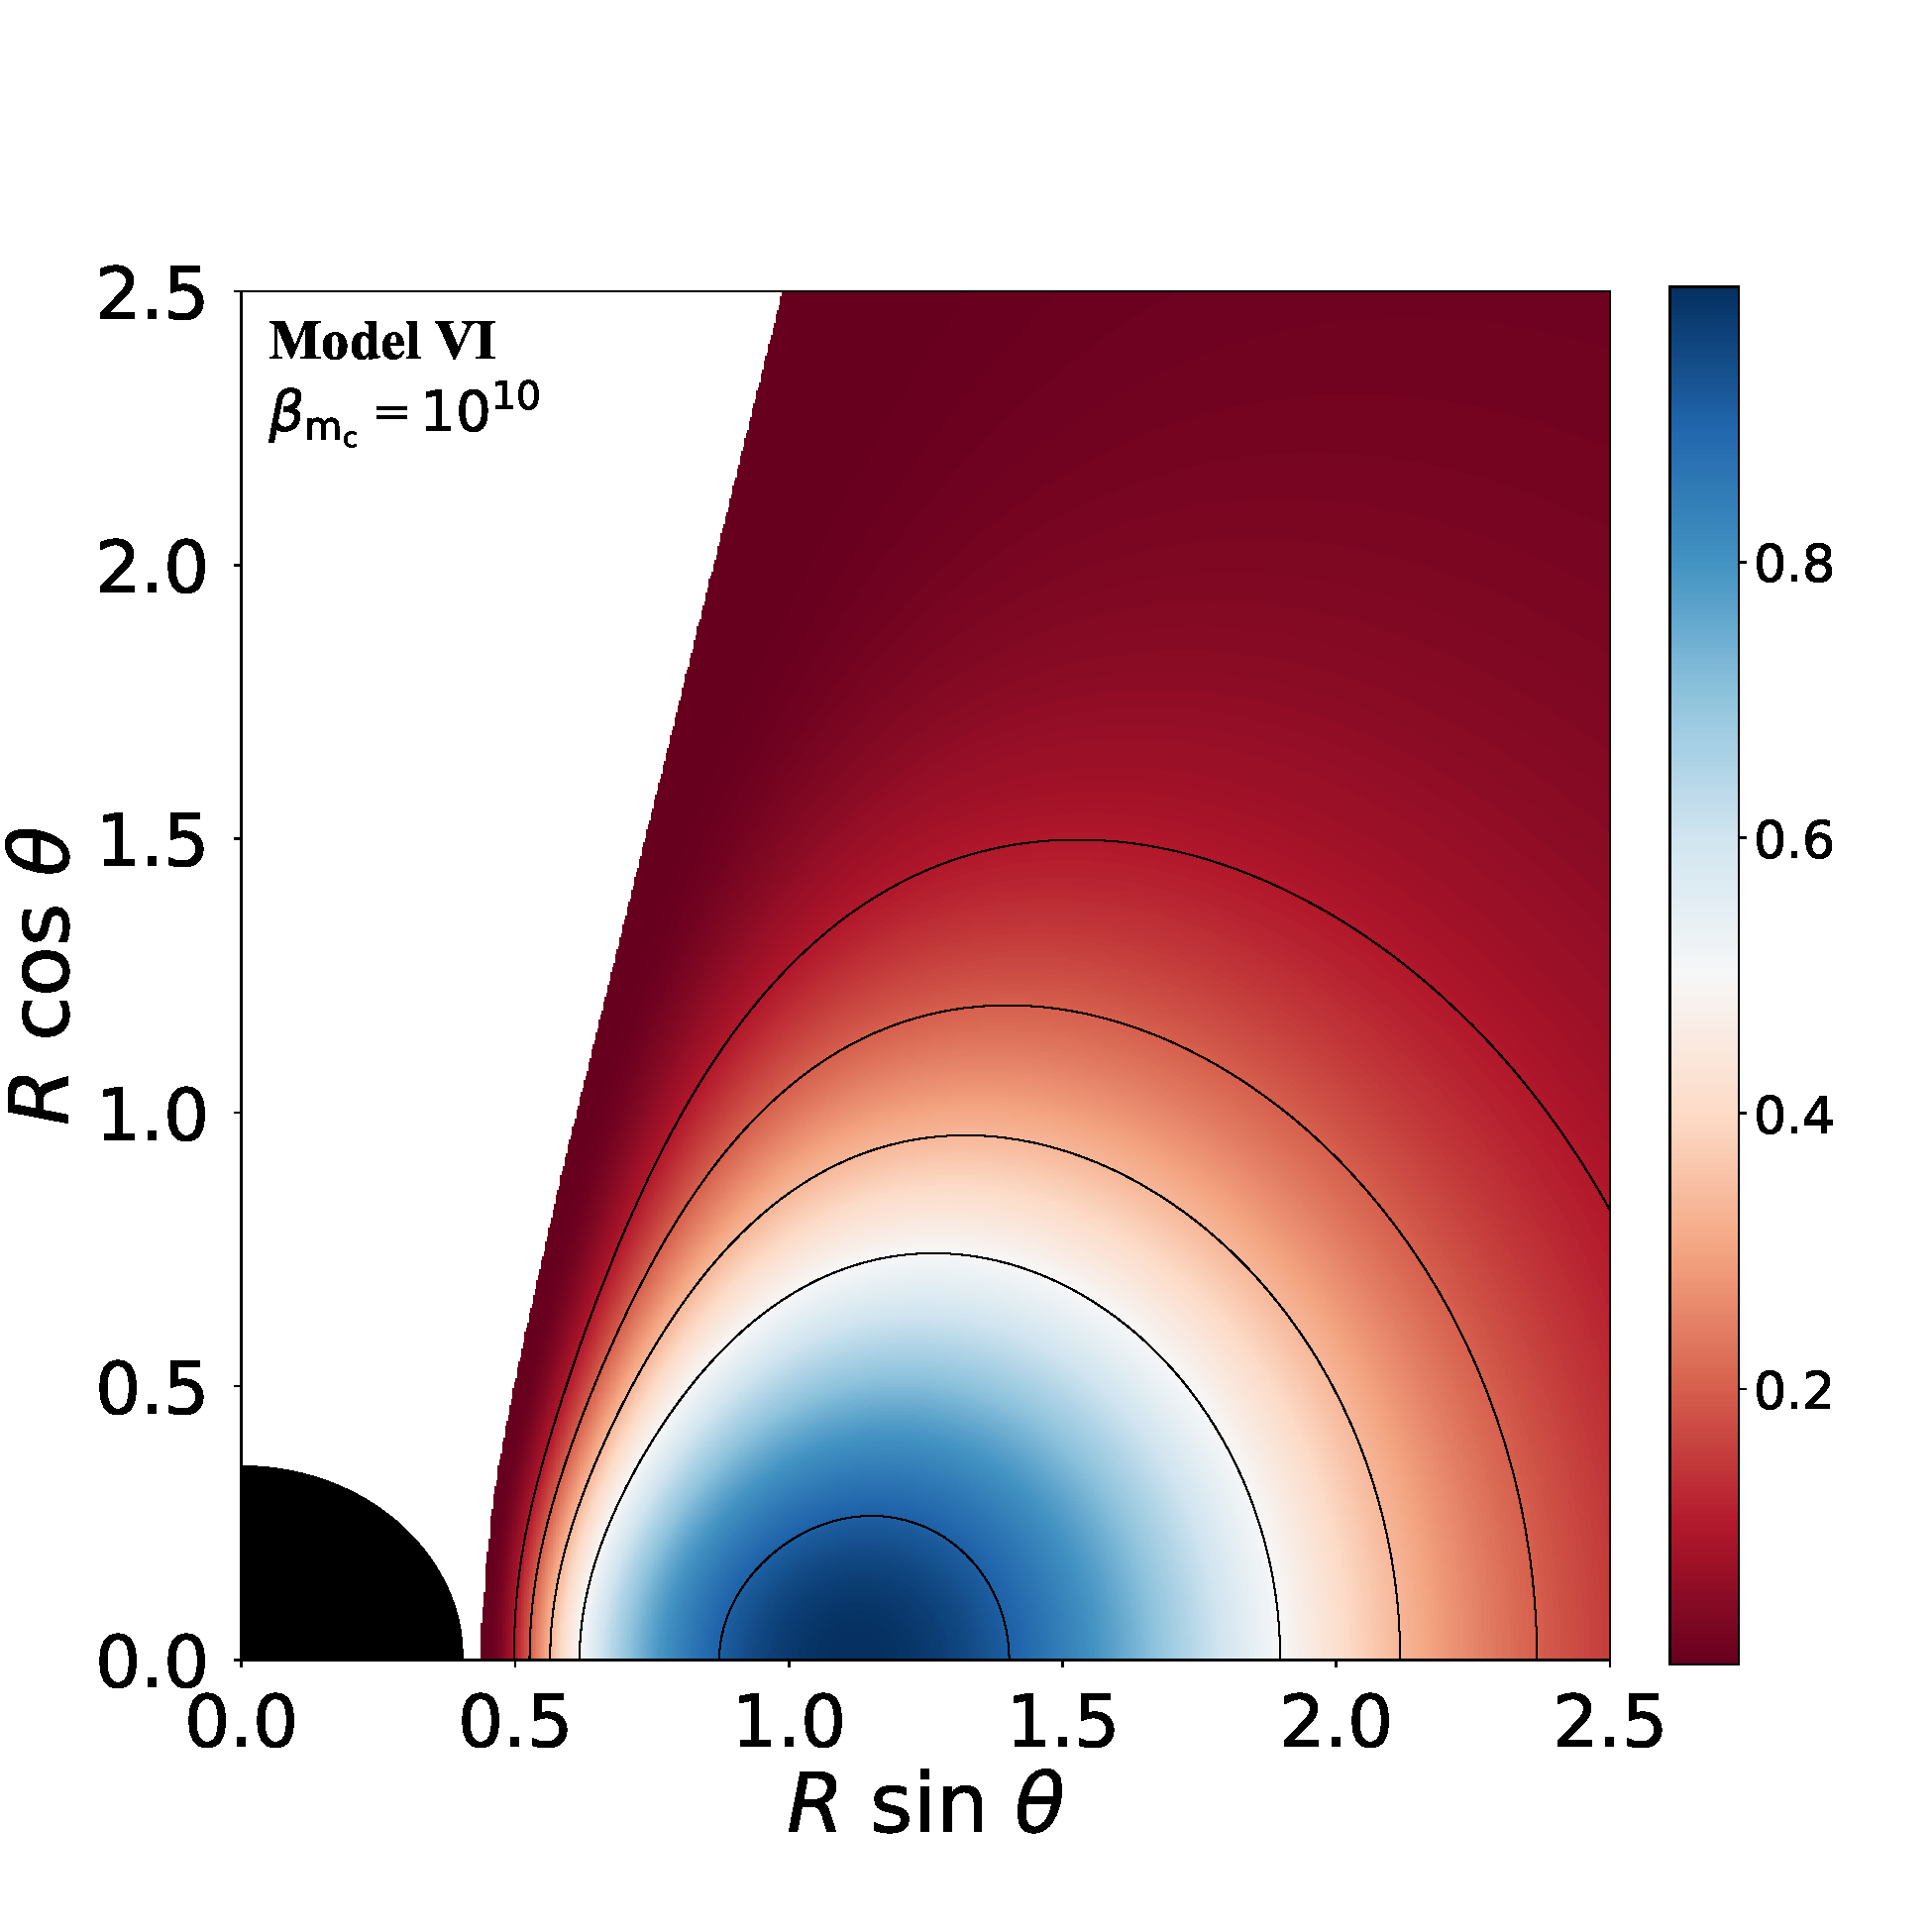
\includegraphics[scale=0.14]{figures/fig4_VI_10.pdf}
\hspace{-0.3cm}
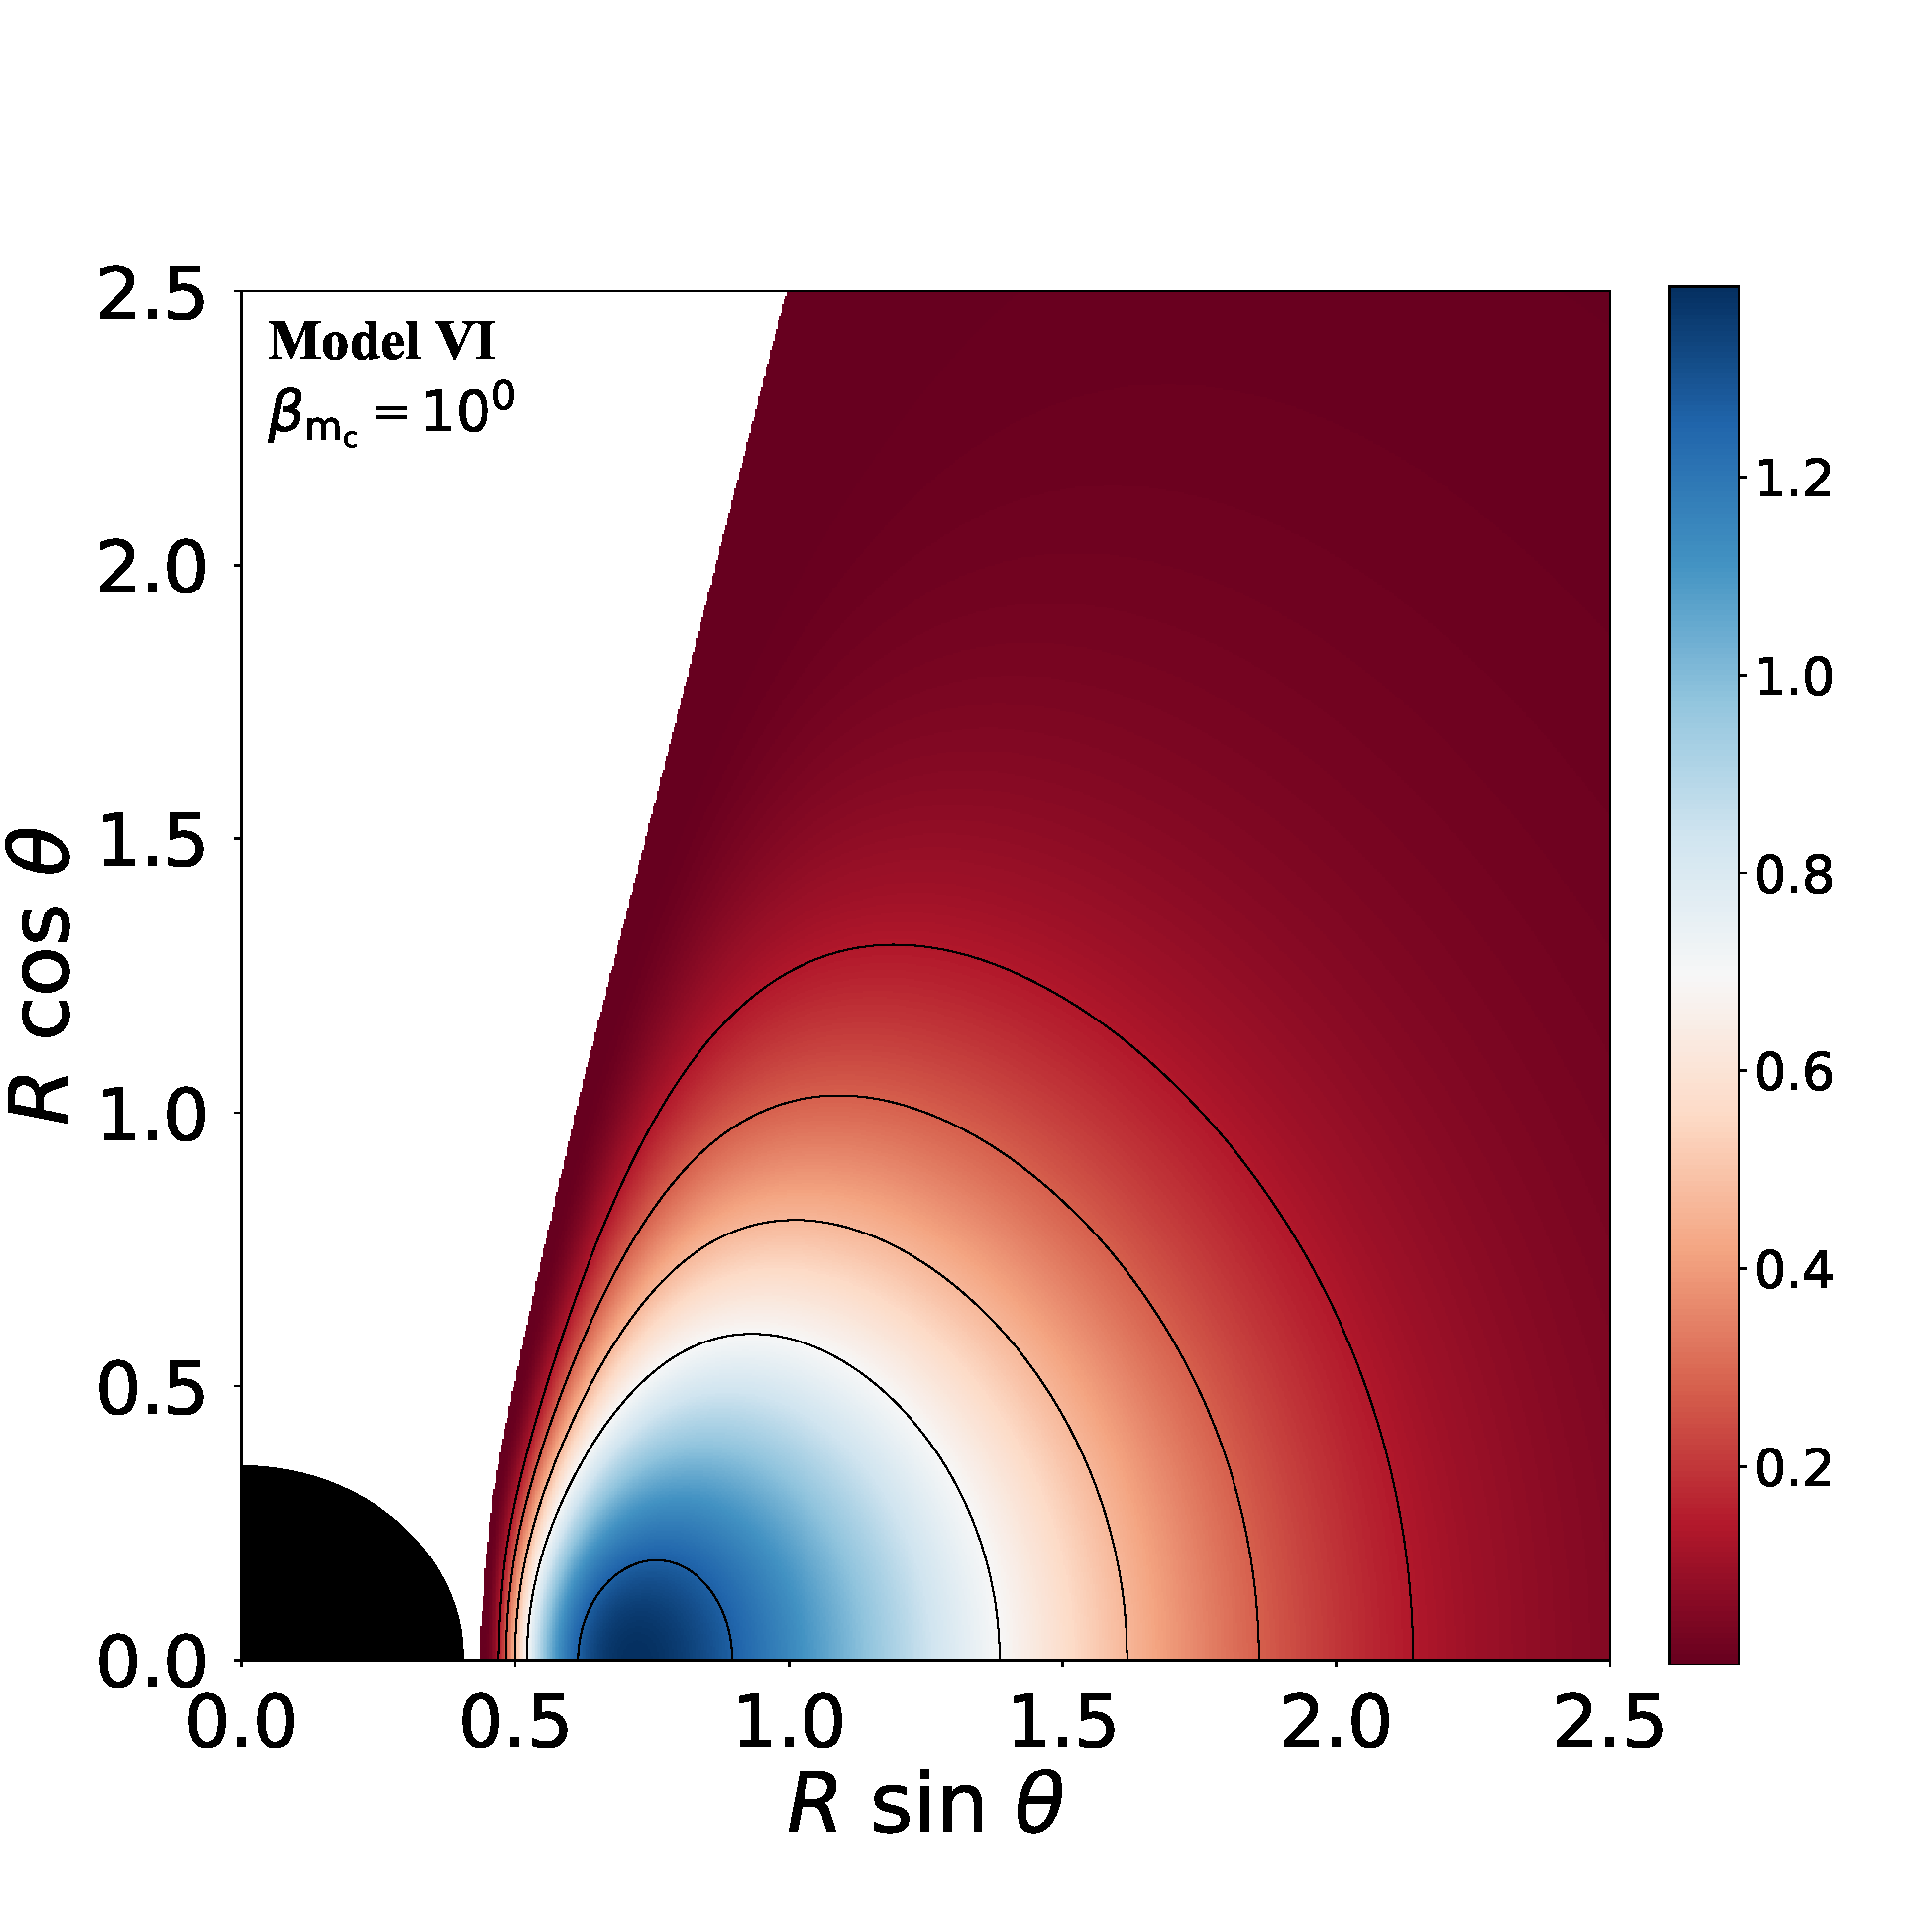
\includegraphics[scale=0.14]{figures/fig4_VI_1.pdf}
\hspace{-0.2cm}
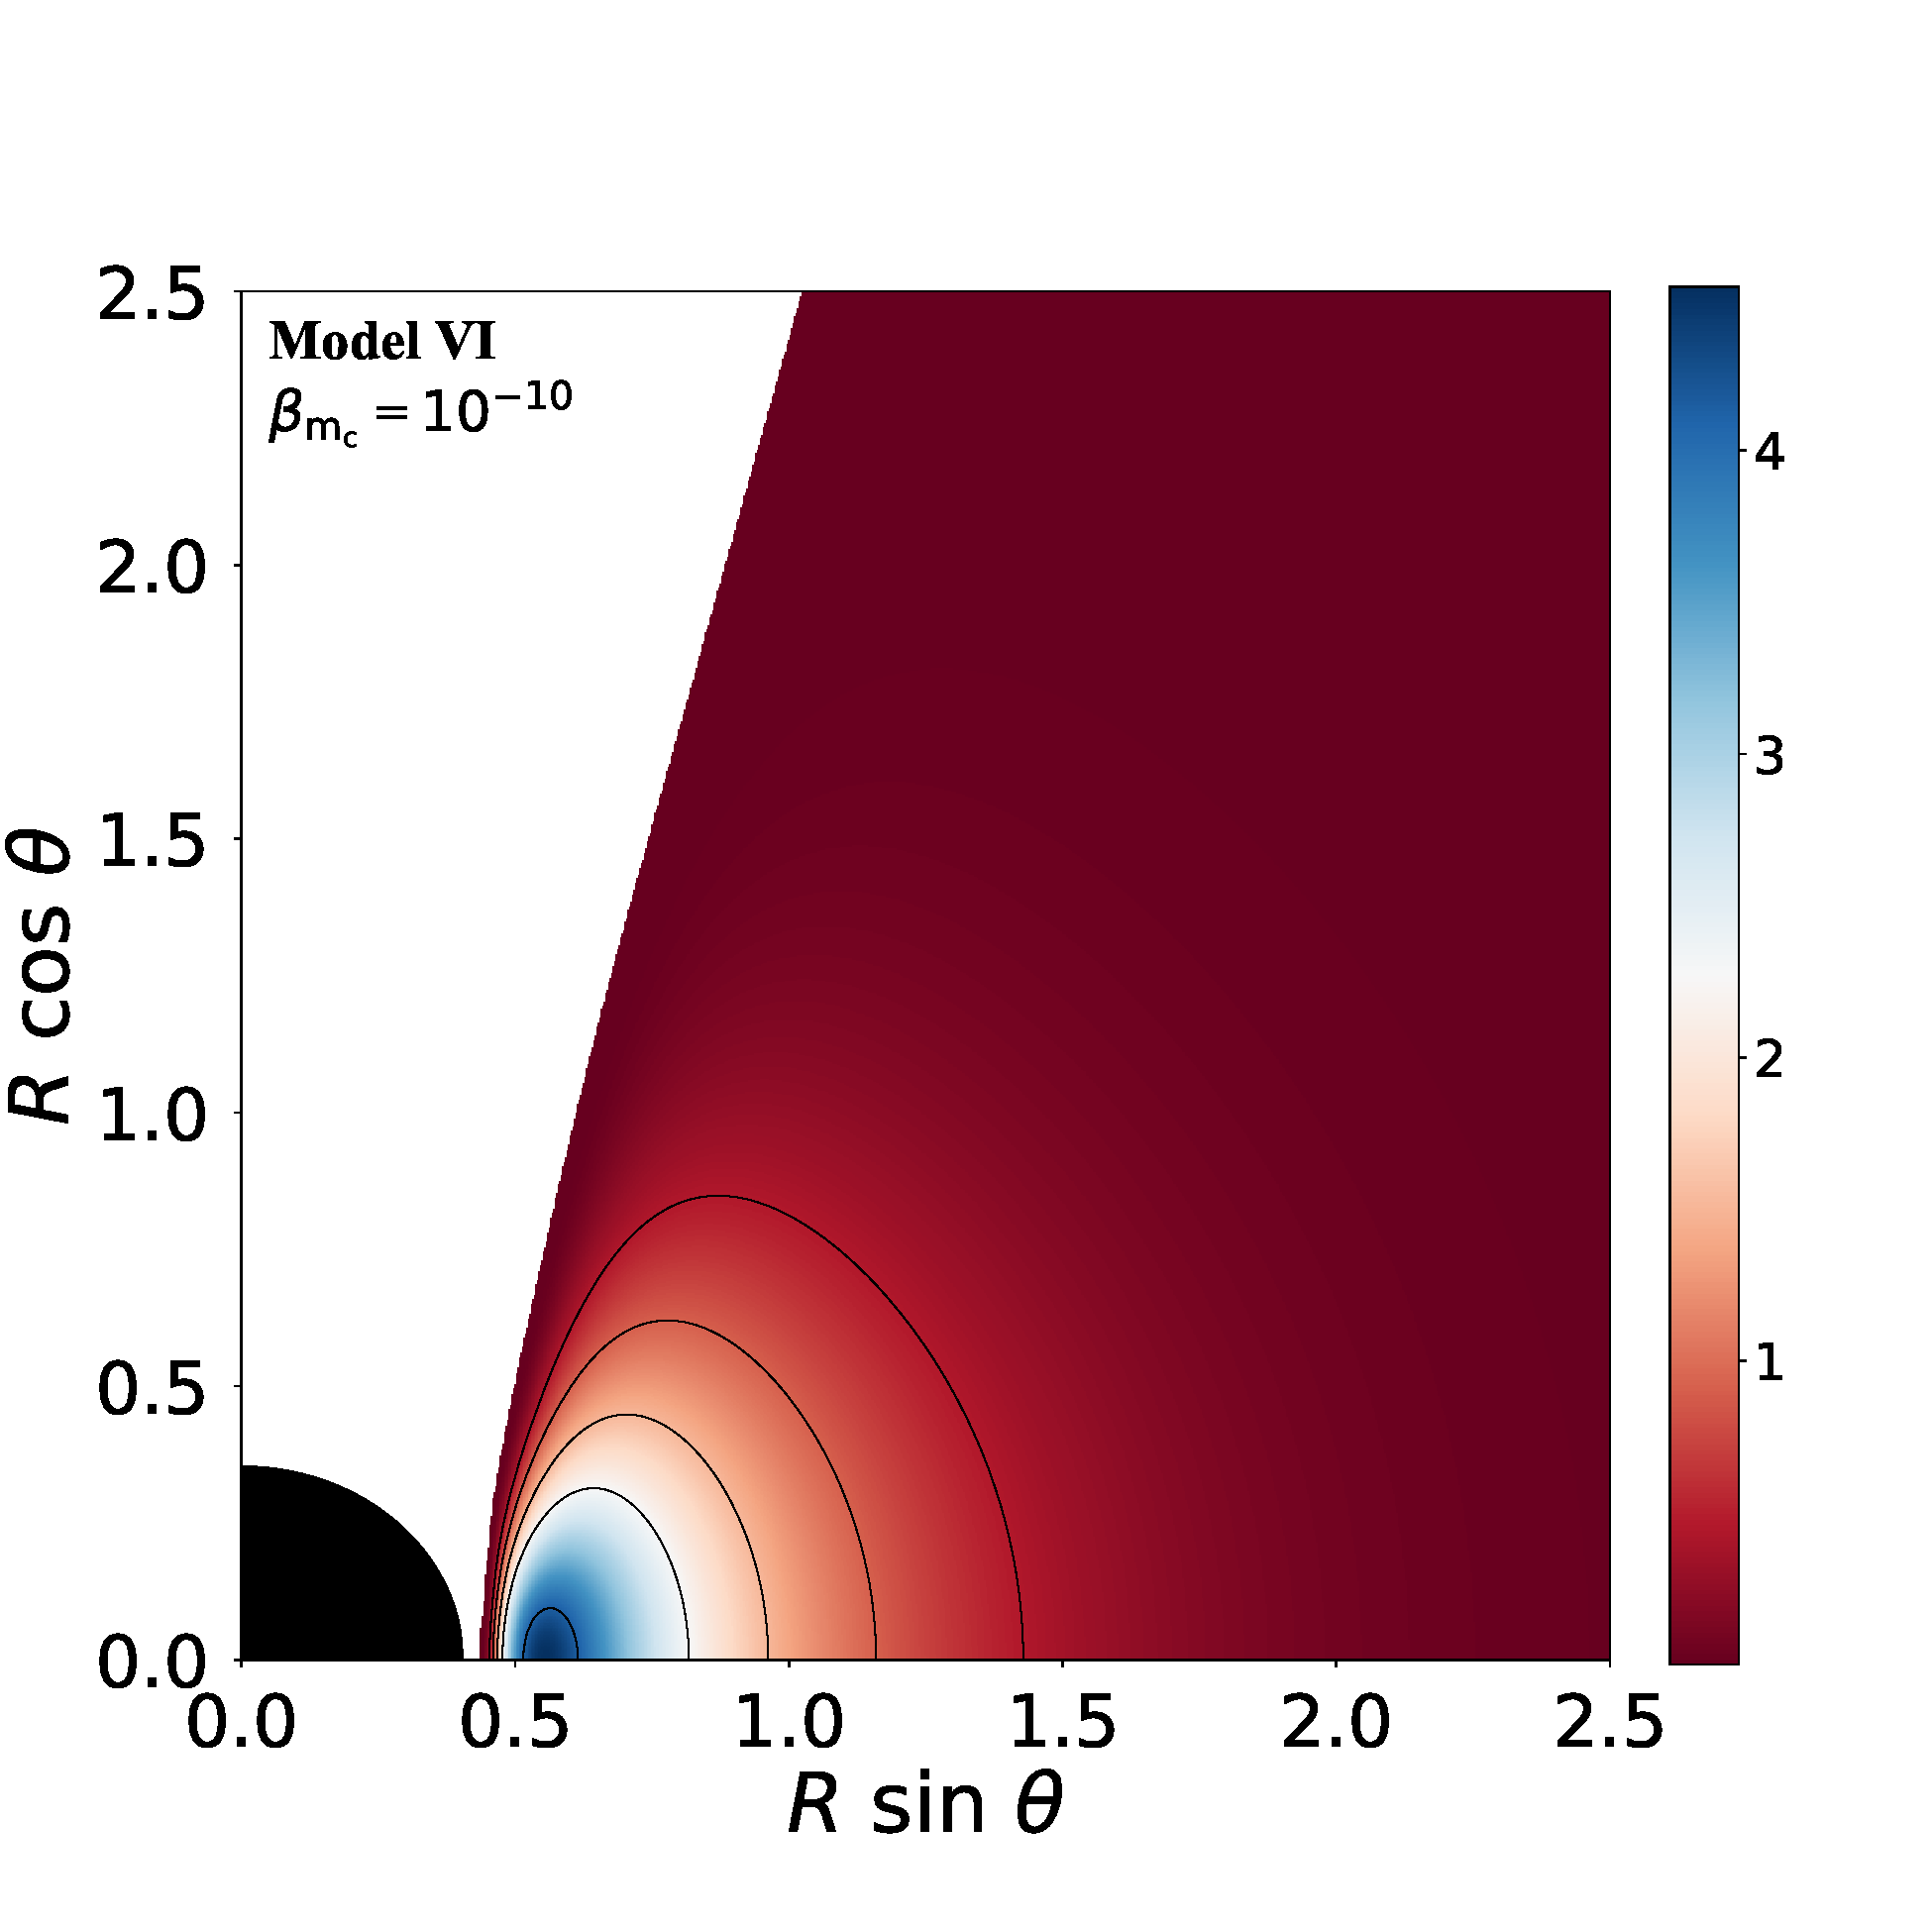
\includegraphics[scale=0.14]{figures/fig4_VI__10.pdf}
\\
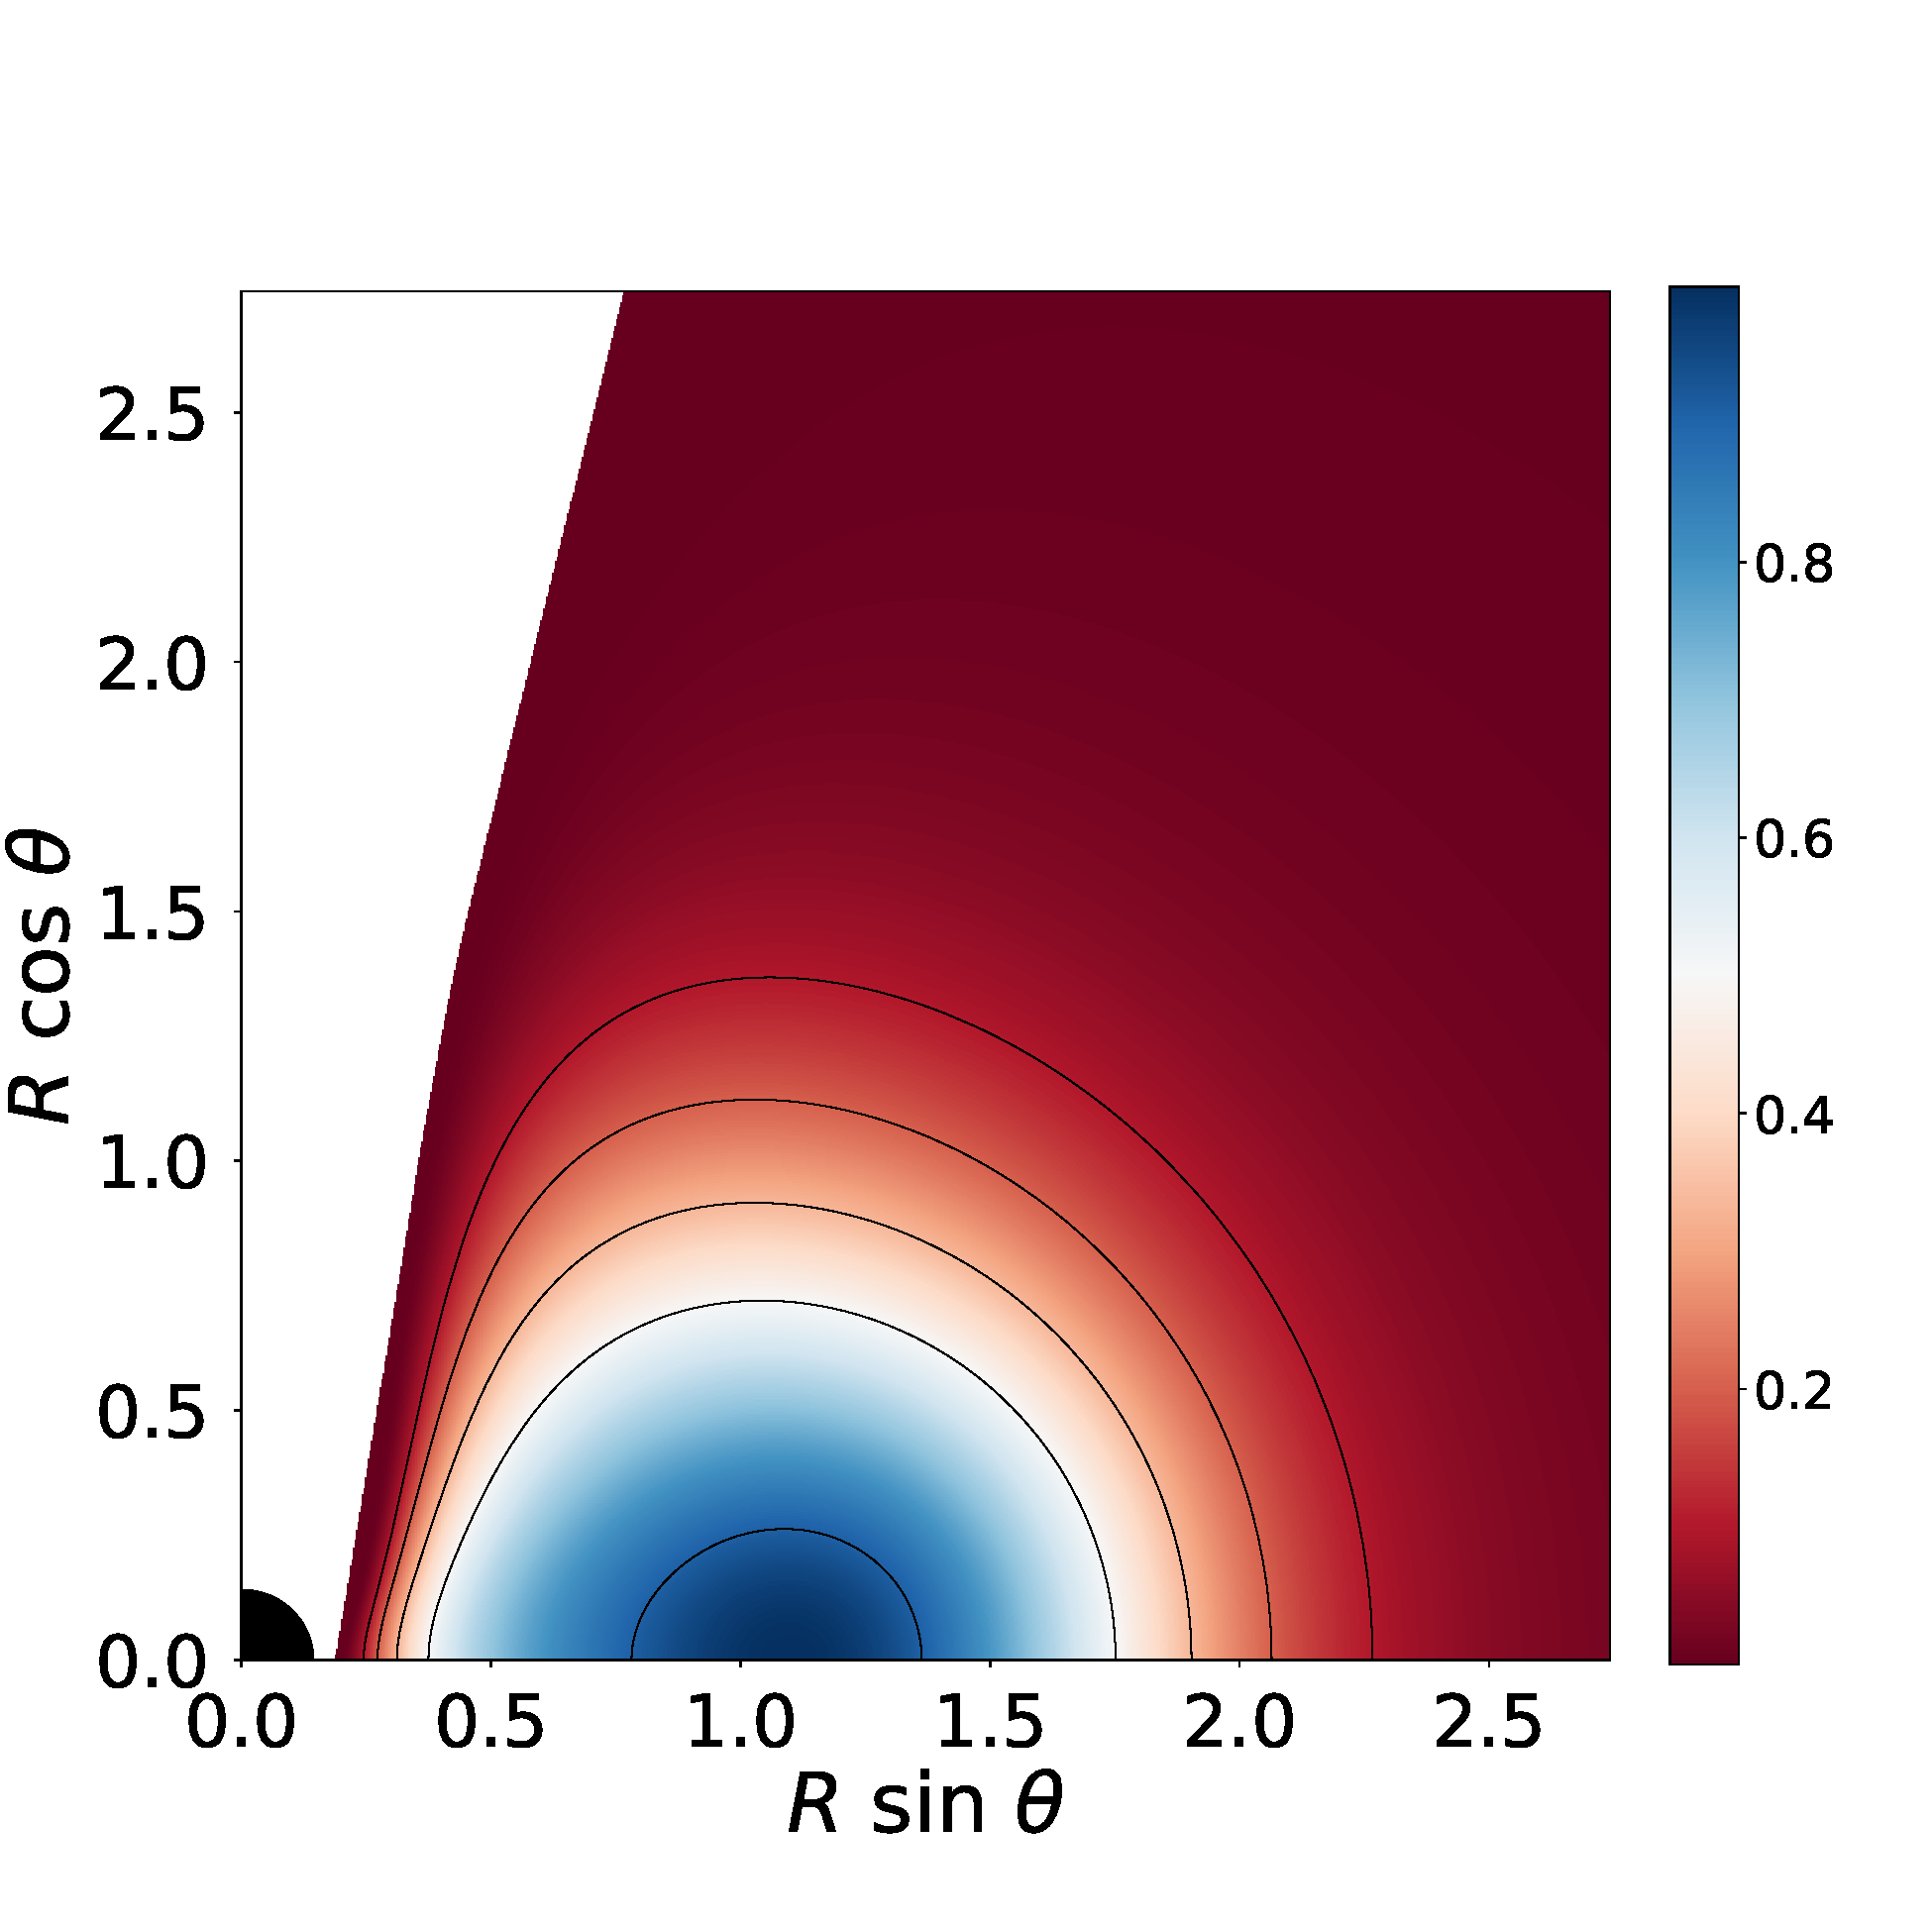
\includegraphics[scale=0.14]{figures/fig4_VII_10.pdf}
\hspace{-0.3cm}
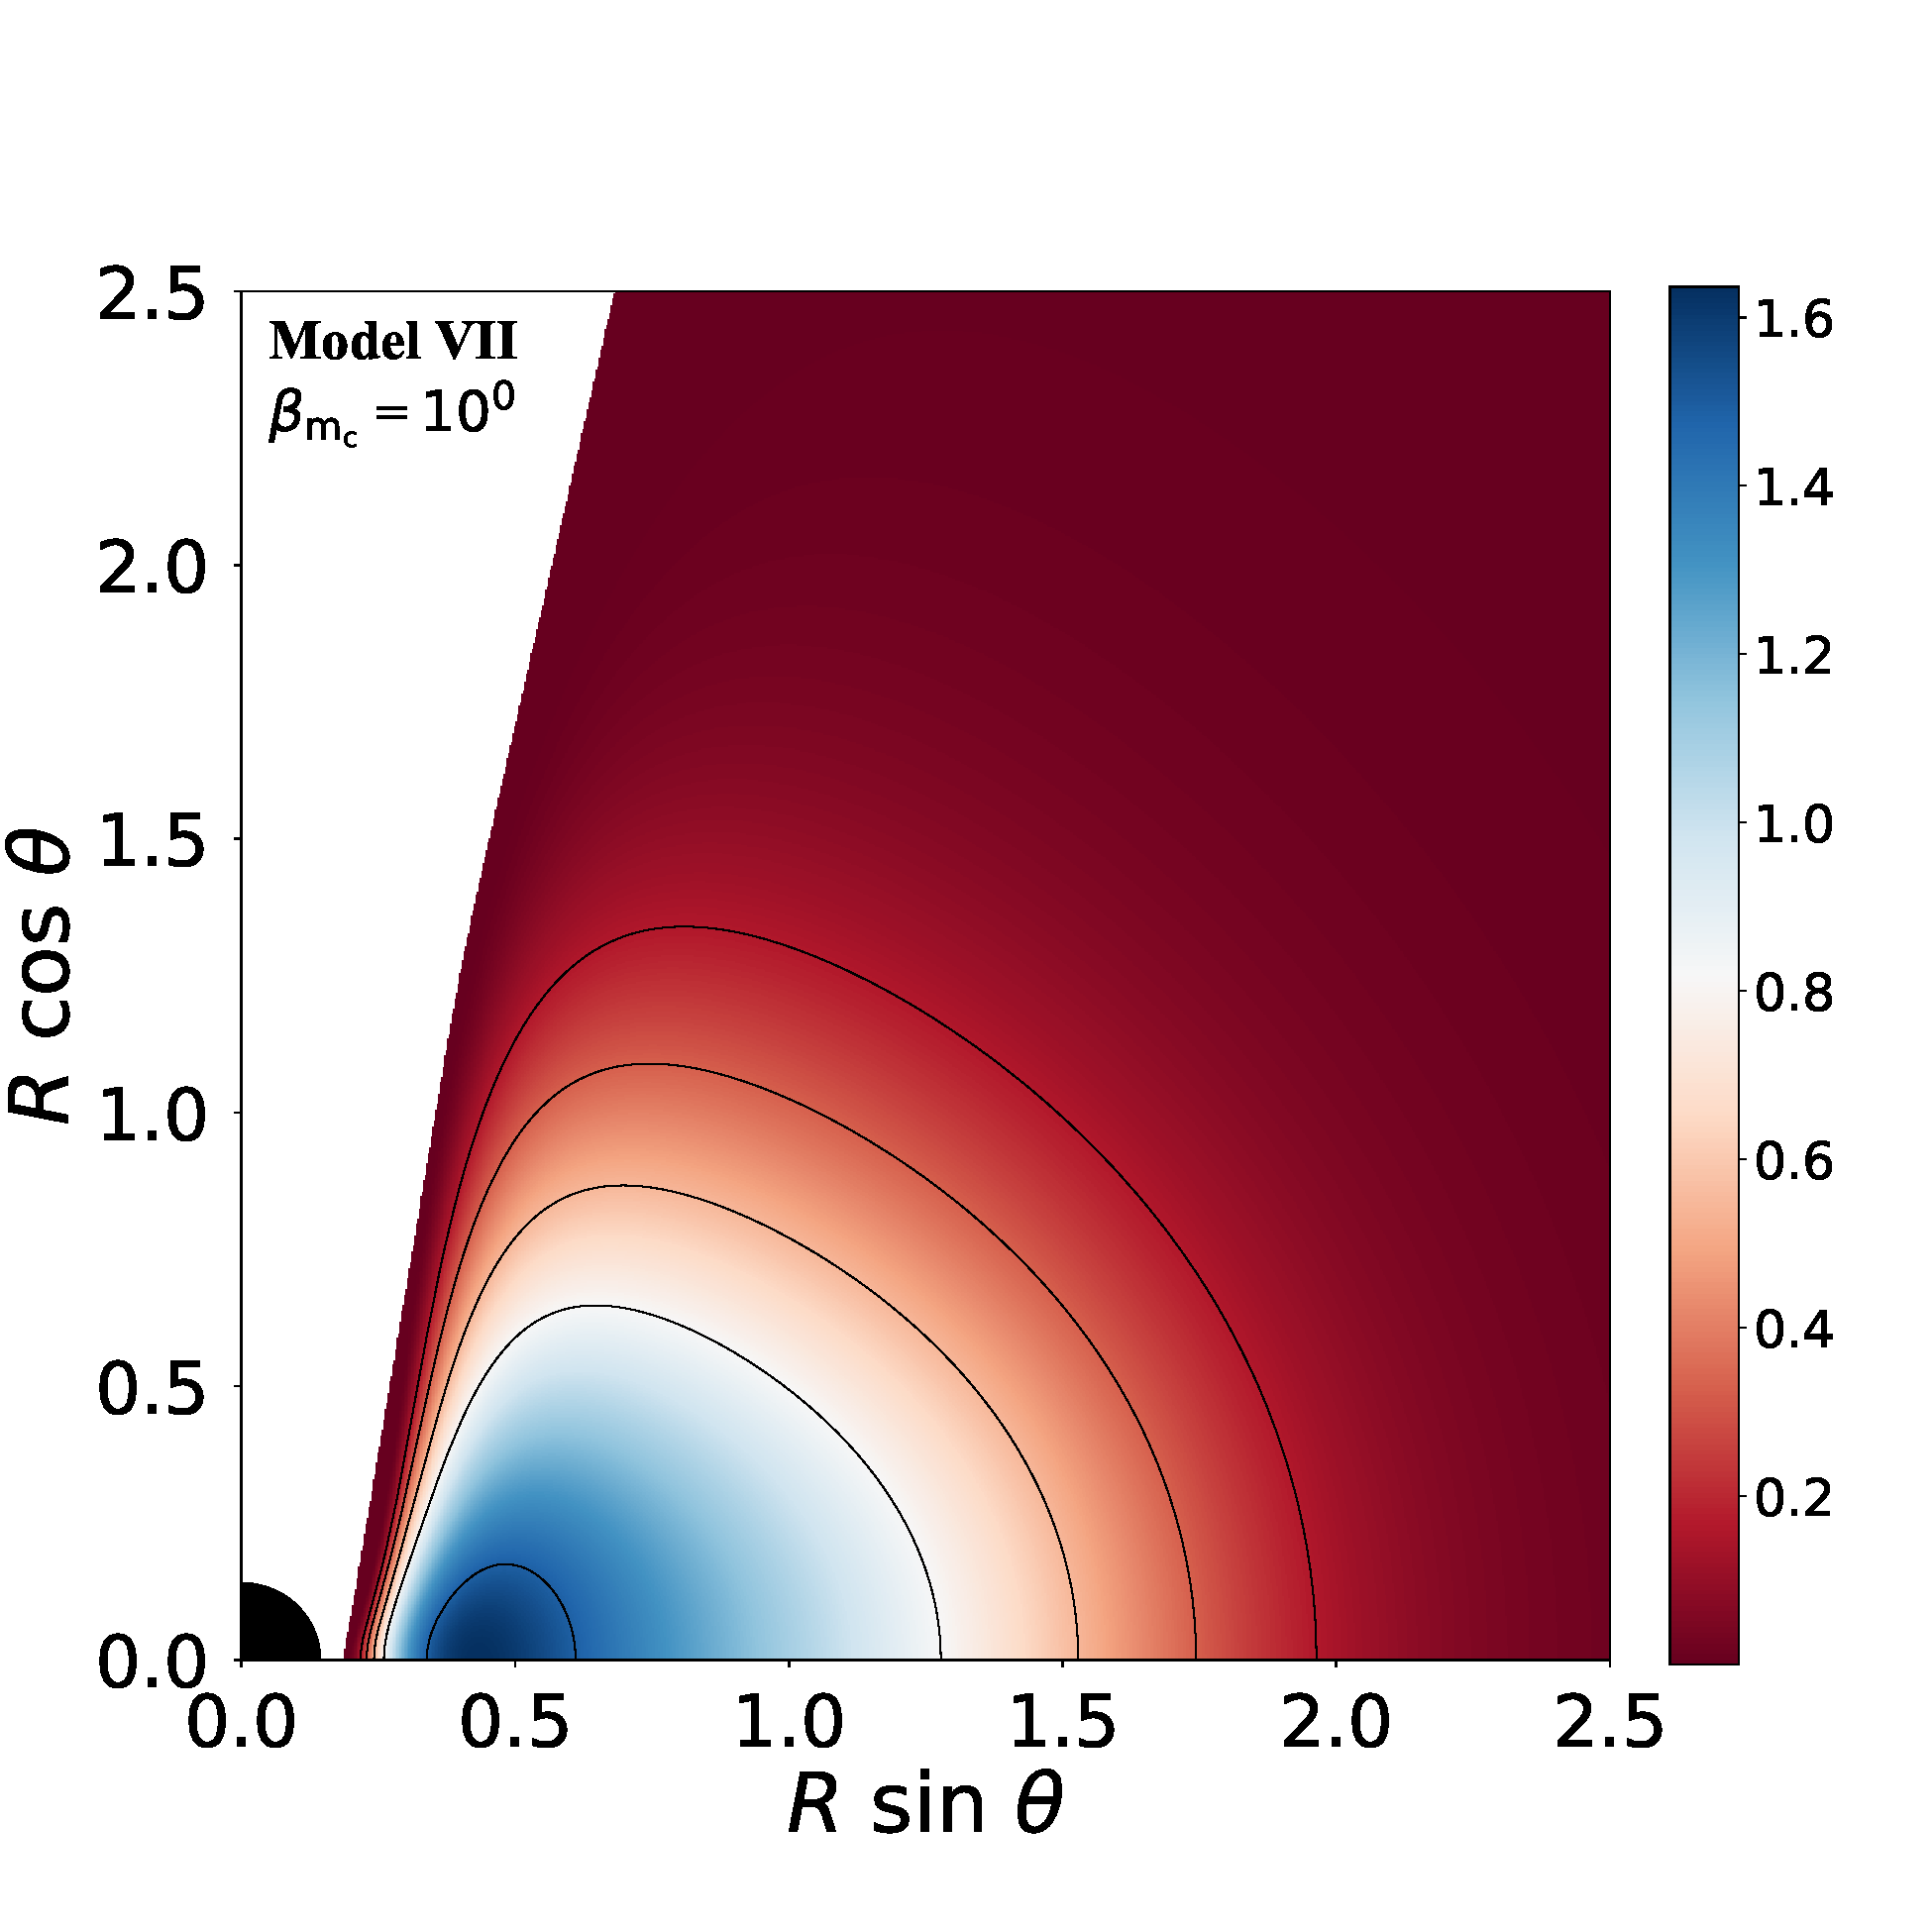
\includegraphics[scale=0.14]{figures/fig4_VII_1.pdf}
\hspace{-0.2cm}
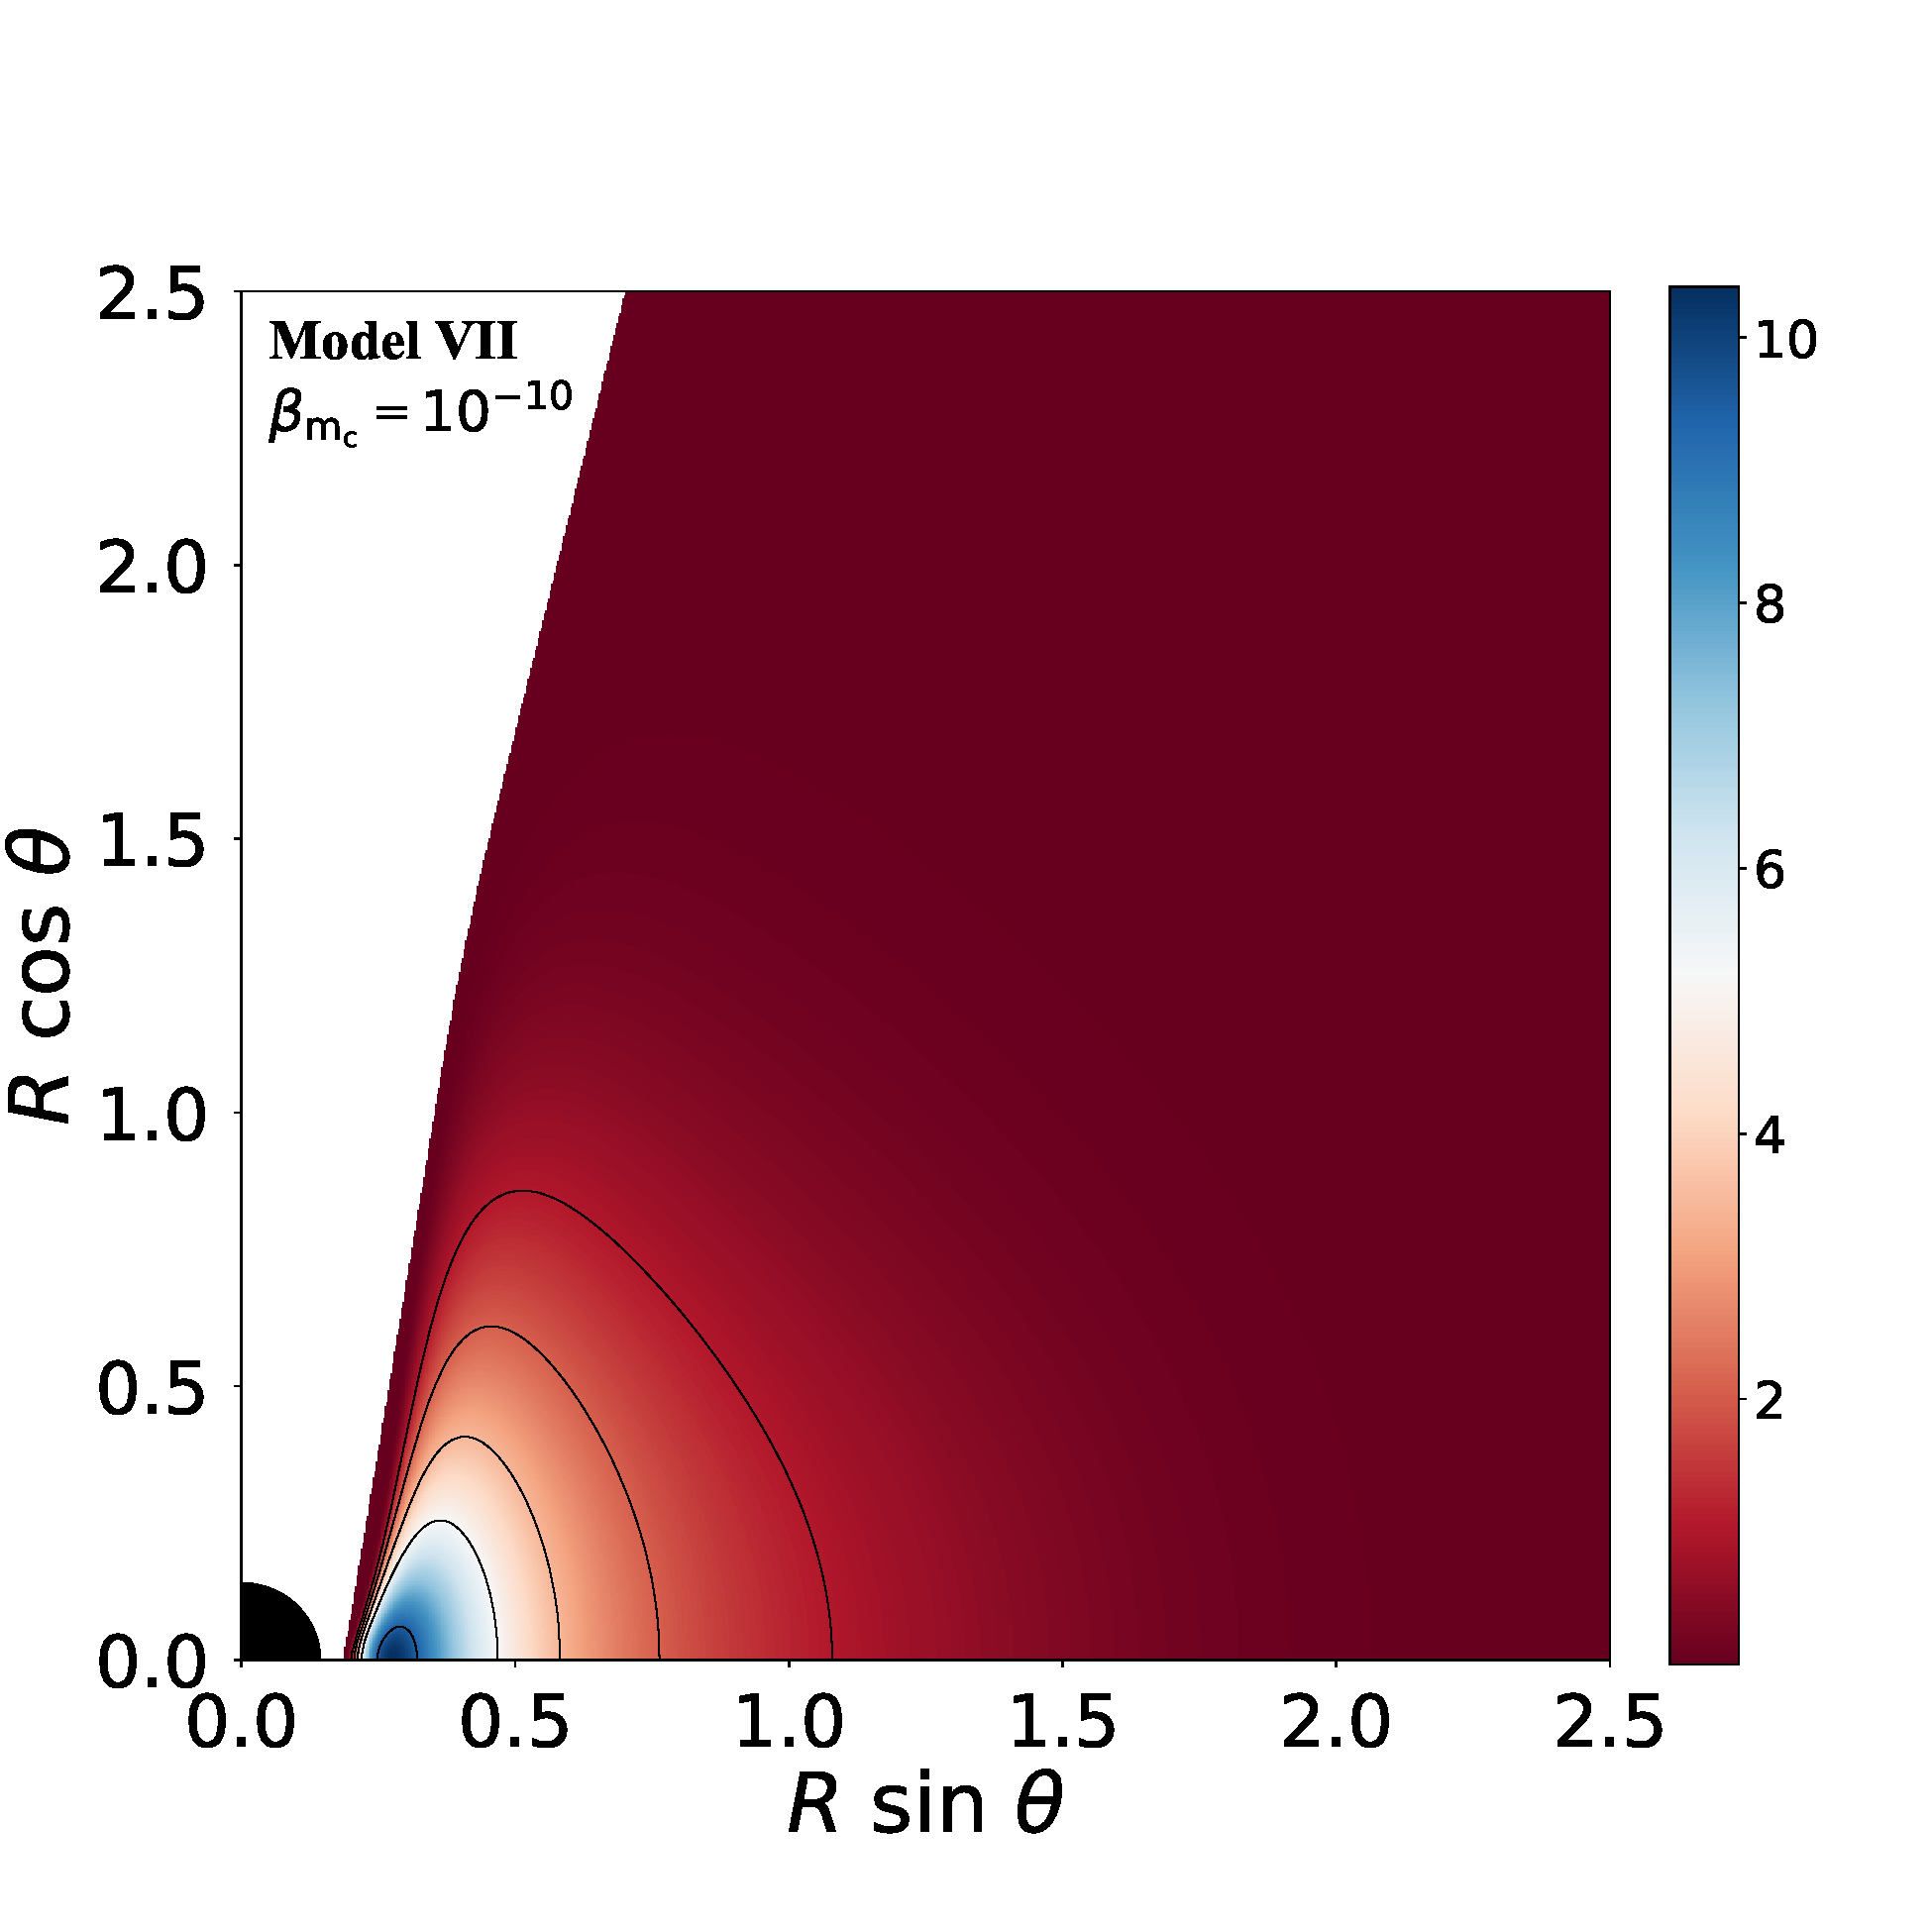
\includegraphics[scale=0.14]{figures/fig4_VII__10.pdf}
\hspace{-0.2cm}
\caption{Same as Fig.~\ref{models_II} but using the perimetral radial coordinate $R$. \tf{Same comment as in the previous figure.}}
\label{models_peri_II}
\end{figure*}



%%%%%%%%%%%%%%%%%%%%%%%%%%%%%%%%%%%%
\subsection{Distribution of angular momentum in the disk}
%%%%%%%%%%%%%%%%%%%%%%%%%%%%%%%%%%%%

Equilibrium models of thick disks around Kerr BHs are built assuming that the spacetime metric and the fluid fields are stationary and  axisymmetric (see, e.g.~\cite{Font:2002,Daigne:2004,Gimeno-Soler:2017} and references therein). For disks around KBHsSH we can follow the same approach as the metric ansatz given by Eq.~(\ref{metric}) is stationary and axisymmetric.

We start by introducing the specific angular momentum $l$ and the angular velocity $\Omega$ employing the standard definitions,
\begin{equation}
l = - \frac{u_{\phi}}{u_t}, \;\;\; \Omega = \frac{u^{\phi}}{u^t},
\end{equation}
where $u^{\mu}$ is the fluid four-velocity.
The relationship between $l$ and $\Omega$ is given by the equations
\begin{equation}
l = - \frac{\Omega g_{\phi\phi} + g_{t\phi}}{\Omega g_{t\phi} + g_{tt}}, \;\;\; \Omega = - \frac{l g_{tt} + g_{t\phi}}{l g_{t\phi} + g_{\phi\phi}},
\end{equation}
where we are assuming circular motion, i.e.~the four-velocity can be written as
\begin{equation}
u^{\mu} = (u^t, 0, 0, u^{\phi})\,.
\end{equation}

The approach we followed in~\cite{Gimeno-Soler:2017} for the angular momentum distribution of the disks was introduced by~\cite{Qian:2009}, and it is characterized by three free parameters, $\beta$, $\gamma$, and $\eta$ (see Eq.~(7) in~\cite{Gimeno-Soler:2017}). In this work, for simplicity and to reduce the ample space of parameters, we consider a constant angular momentum distribution, $l(r,\theta) = \mathrm{const}$, which corresponds to setting $\beta=\gamma=0$ in~\cite{Gimeno-Soler:2017}. This choice also allows for the presence of a cusp (and hence matter accretion onto the black hole) and a centre.  \tf{We should explain/motivate why we change our approach in this paper.}\sg{We limit this study to the constant angular momentum case to limit the parameter space, as the main aim of this paper is to study the dependence of the characteristics of magnetised discs with respect to the KBHSH spacetime.} Following~\citep{Daigne:2004}, the specific value of the angular momentum corresponding to bound fluid elements ($-u_t<1$) is computed as the minimum of the following equation
\begin{equation}\label{eq:mb_ang_mom}
l^{\pm}_{\mathrm{b}}(r, \theta) = \frac{g_{t\phi} \pm \sqrt{ (g_{t\phi}^2-g_{tt}g_{\phi\phi})  (1+g_{tt}) } }{-g_{tt}}
\end{equation}
where the plus sign corresponds to prograde orbits and the minus sign to retrograde orbits. Our convention is that the angular momentum of the BH is positive and the matter of the disk rotates in the positive (negative) direction of $\phi$ for a prograde (retrograde) disk.
Equation~(\ref{eq:mb_ang_mom}) is given by~\citep{Daigne:2004} for Kerr BHs, but it is valid for any stationary and axisymmetric spacetime. For prograde motion, the function has a minimum outside the event horizon. The location of this minimum corresponds with the marginally bound orbit $r_{\mathrm{mb}}$, and the angular momentum corresponds to the Keplerian angular momentum $l_{\mathrm{mb}}$ at that point. We show the proof of this statement in Appendix~\ref{ang_mom_appendix}. \tf{Is there an Appendix A?}.

%%%%%%%%%%%%%%%%
\subsection{Magnetized disks}
%%%%%%%%%%%%%%%%

To account for the magnetic field in the disks we use the procedure described by~\cite{Komissarov:2006,Montero:2007}. We write the equations of ideal general relativistic MHD as the following conservation laws, $\nabla_{\mu} T^{\mu\nu} = 0$, $\nabla_{\mu} \,^\ast F^{\mu\nu} = 0$, and 
$\nabla_{\mu} (\rho u^{\mu}) = 0$, 
where $\nabla_{\mu}$ is the covariant derivative and
\begin{equation}\label{eq:e-m_tensor}
T^{\mu\nu} = (\rho h + b^2)u^{\mu}u^{\nu} + (p + p_{\mathrm{m}})g^{\mu\nu} - b^{\mu}b^{\nu},
\end{equation}
is the energy-momentum tensor of a magnetized perfect fluid, $h$, $\rho$, $p$, and $p_{\mathrm{m}}$ being the fluid specific enthalpy, density, fluid pressure, and magnetic pressure, respectively, the latter defined as $p_{\mathrm{m}} = b^2/2$. The ratio of fluid pressure to magnetic pressure defines the magnetization parameter $\beta_{\mathrm{m}} = p/p_{\mathrm{m}}$.
Moreover, $^\ast F^{\mu\nu} = b^{\mu}u^{\nu} - b^{\nu}u^{\mu}$ is the (dual of the) Faraday tensor relative to an observer with 
four-velocity $u^{\mu}$, and $b^{\mu}$ is the magnetic field in that frame, with
$b^2=b^{\mu}b_{\mu}$ (see~\cite{Anton:2006} for further details). Assuming the magnetic field is purely azimuthal, i.e.~$b^r = b^{\theta} = 0$,
and taking into account that the flow is stationary and axisymmetric, the conservation of the current density and of the Faraday tensor follow. Contracting the divergence of Eq.~\eqref{eq:e-m_tensor} with the projection tensor $h^{\alpha}_{\,\,\beta} = \delta^{\alpha}_{\,\,\beta} + u^{\alpha}u_{\beta}$, we arrive at
\begin{equation}
(\rho h + b^2)u_{\nu}\partial_i u^{\nu} + \partial_i\left(p + \frac{b^2}{2}\right) - b_{\nu}\partial_i b^{\nu}=0\,,
\end{equation}
where $i = r, \theta$. This equation can be rewritten in terms of the specific angular momentum $l$ and of the angular velocity $\Omega$, 
\begin{equation}\label{eq:diff_ver}
\partial_i(\ln u_t|) - \frac{\Omega \partial_i l}{1-l\Omega} + \frac{\partial_i p}{\rho h} + \frac{\partial_i(\mathcal{L}b^2)}{2\mathcal{L}\rho h} = 0\,,
\end{equation}
where $\mathcal{L} = g_{t\phi}^2 - g_{tt}g_{\phi\phi}$.

To integrate Eq.~\eqref{eq:diff_ver} we need to assume an equation of state (EOS). We assume a polytropic EOS of the form
\begin{equation}\label{eq:eos_fluid}
p = K \rho^{\Gamma},
\end{equation}
with $K$ and $\Gamma$ constants.
 By introducing the definitions $\tilde{p}_{\mathrm{m}} = \mathcal{L} p_{\mathrm{m}}$, $w = \rho h$ and $\tilde{w} = \mathcal{L} (w)$, we can write equations equivalent to Eq.~\eqref{eq:eos_fluid} for both $\tilde{p}_{\mathrm{m}}$ and $p_{\mathrm{m}}$
\begin{eqnarray}
\label{eq:eos_mag_tilde}
\tilde{p}_{\mathrm{m}} &=& M \tilde{w}^q,
\\
p_{\mathrm{m}} &=& M \mathcal{L}^{q-1} (\rho h)^q,
\end{eqnarray}
where $M$ and $q$ are constants. Then we can integrate Eq.~\eqref{eq:diff_ver} as
\begin{equation}\label{eq:final}
W - W_{\mathrm{in}} + \ln \left(1 + \frac{\Gamma K}{\Gamma +1}\rho^{\Gamma -1}\right) + \frac{q}{q-1}M(\mathcal{L}\rho h)^{q-1}=0,
\end{equation}
where $W \equiv \ln |u_t|$ stands for the (gravitational plus centrifugal) potential and  $W_{\mathrm{in}}$ is the potential at the inner edge of the disk.

We can also define the total energy density for the torus, $\rho_{\mathrm{T}}=-T^t_t + T^i_i$, and for the scalar field, $\rho_{\mathrm{SF}}=-(T_{\mathrm{SF}})^t_t + (T_{\mathrm{SF}})^i_i$. These are given by
\begin{eqnarray}\label{eq:torus_energy_density}
\rho_{\mathrm{T}} &=&  \frac{\rho h (g_{\phi\phi} - g_{tt} l^2)}{g_{\phi\phi} + 2 g_{t\phi} l + g_{tt} l^2} + 2 (p + p_{\mathrm{m}}),
\\
\rho_{\mathrm{SF}} &=&  2 \left(\frac{2 e^{2 F_0} w (w-m W)}{N} - \mu^2\right) \phi^2.
\end{eqnarray}

%
%\begin{equation}\label{eq:torus_energy_density}
%\rho_{\mathrm{T}} = -T^t_t + T^i_i = \frac{\rho h (g_{\phi\phi} - g_{tt} l^2)}{g_{\phi\phi} + 2 g_{t\phi} l + g_{tt} l^2} + 2 (p + p_{\mathrm{m}}),
%\end{equation}
%and
%\begin{equation}\label{eq:SF_energy_density}
%\rho_{\mathrm{SF}} = -(T_{\mathrm{SF}})^t_t + (T_{\mathrm{SF}})^i_i = 2 \left(\frac{2 e^{2 F_0} w (w-m W)}{N} - \mu^2\right) \phi^2.
%\end{equation}

From the previous discussion it becomes apparent that the number of parameters defining the disk models is fairly large. In order to reduce the sample, in this work we set the mass of the scalar field $\mu = 1$, the specific angular momentum to $l = l_{\mathrm{mb}}$, the inner radius of the disk to $r_{\mathrm{in}} = r_{\mathrm{mb}}$, the exponents of the polytropic EOS to $q = \Gamma = 4/3$, and the density at the centre of the disk $\rho_{\mathrm{c}} = 1$.Thus, we leave the magnetization at the centre $\beta_{\mathrm{m_c}}$ as the only free parameter for each model of KBHsSH. With this information we can compute all relevant physical quantities.

\tf{We should discuss a bit more the reason for this choice. If $l_{\rm ms}<l<l_{\rm mb}$ and $r_{\rm mb}<r_{\rm cusp}<r_{\rm ms}$ the disk is closed and has a centre and a cusp. If $l=l_{\rm mb}$ and $r_{\rm cusp}=r_{\rm mb}$ the disk has a centre and a cusp, and it is closed at infinity. The models we have built are the latter, right? I wonder if we should have built models not completely filling their Roche lobe, so that they had a finite size. In any case, a comment must be provided here.}
\sg{We choose this value for the angular momentum and the inner radius of the disc to allow discs with a cusp and a centre that also are marginally stable (a small perturbation can trigger accretion into the black hole). Also, the thermodynamical quantities reach its maximum for this particular choice of angular momentum and inner radius of the disc (as they are related to the total potential well $|\Delta W|$). This also means that the resulting discs will be semi-infinite (they are closed at infinity), this is not a source of concern, as the external layers of the disc have extremely low density. (not sure about the relevance of the last part...)}

\tf{We also have to emphasize somewhere in the paper that we do not fix $h=1$. This is an important difference with respect to the work of~\cite{Vincent:2016}.}

%%%%%%%%%%%%
\section{Methodology}
\label{procedure}
%%%%%%%%%%%%

\tf{Probably we do not need to have two subsections in this section, but just one. The description of the methodology is very
poor now. It needs a lot of rewriting.}
\sg{I have serious doubts about this section, as I am not really certain that we need to provide an explanation for some specific parts (that are pretty obvious anyway) Perhaps I should go into detail for the numerical part? (e.g. that Eq.~\eqref{eq:final} is a trascendental equation and we are bound to solve it numerically with the bisection method for each cell of our numerical grid)}

% %%%%%%%%%%%%%%%%
% \subsection{Building the disks}
% %%%%%%%%%%%%%%%%

% To construct our models we first find the specific angular momentum $l$ and the radius of the cusp $r_{\mathrm{cusp}}$ as the minimum value of Eq.~\eqref{eq:mb_ang_mom} and the radial location of said minimum outside the event horizon, respectively. This choice of angular momentum implies $r_{\mathrm{cusp}} = r_{\mathrm{mb}}$, $l = l_{\mathrm{K}}(r_{\mathrm{mb}})$, and $W_{\mathrm{in}} = 0$. Next, we can compute the gravitational plus centrifugal potential distribution as $W(r, \theta) \equiv \ln |u_t|$. Considering this, and that we can write the magnetic pressure at the centre as
% \begin{equation}
% p_{\mathrm{m_c}} = M \mathcal{L}^{q-1} \left(1 + \frac{\Gamma K}{\Gamma +1}\right)^q = \frac{K}{\beta_{\mathrm{m_c}}},
% \end{equation}
% where we have taken into account that $\rho_{\mathrm{c}} = 1$, that the pressure at the center is $p_{\mathrm{c}} = K$ and the specific enthalpy can be written as $h = 1 + \frac{\Gamma K}{\Gamma +1}\rho^{\Gamma -1}$. \tf{The previous sentence reads a bit strange.} Replacing this into Eq.~\eqref{eq:final} we arrive at an equation for the polytropic constant $K$
% \begin{equation}\label{eq:K_eq}
% W_{\mathrm{c}} + \ln \left(1 + \frac{\Gamma K}{\Gamma +1}\right) + \frac{q}{q-1}\frac{K/\beta_{\mathrm{m_c}}}{1 + \frac{\Gamma K}{\Gamma +1}} = 0.
% \end{equation}
% Once we have $K$, it is easy to find $p_{\mathrm{m}}$, $M$ and $h_{\mathrm{c}}$ with the definition of the magnetization parameter at the center $\beta_{\mathrm{m_c}}$, the equation~\eqref{eq:eos_mag} and $h = 1 + \frac{\Gamma K}{\Gamma +1}\rho^{\Gamma -1}$. With this, we already have all we need in order to compute all the relevant physical quantities inside the disk.

% %%%%%%%%%%%%%%%%%
% \subsection{Numerical method}
% %%%%%%%%%%%%%%%%%

% We start from a uniform numerical grid $(X, \theta)$ (with $x$ being a compactified radial coordinate such as $X = x/(1+x)$ and $x = \sqrt{r^2 - r_{\mathrm{H}}^2}$) with a domain $[0, 1] \times [0, \pi/2]$ and a number of points of $N_X \times N_\theta = 251 \times 30$. Then, we transform and interpolate the grid to end with a non-uniform grid $(r, \theta)$ with a domain $[r_{\mathrm{H}}, 199.2] \times [0, \pi/2]$ and a number of points $N_r \times N_\theta = 2500 \times 300$, this is the grid we use for our computations.

%%%%%%%%%%
\section{Results}
\label{results}
%%%%%%%%%%

%In table~\ref{models_list} we show the different KBHsSH models we will use. As it can be seen, the models go from a Kerr-like model (almost all the mass and angular momentum are stored in BH) to a KBHSH with almost all the mass and angular momentum stored in the scalar field. It is also worth mentioning that, as shown in table~\ref{models_spin_vel} some of the models violate the Kerr bound (in terms of ADM or horizon quantities). This is not worrying because, as shown in~\cite{Herdeiro:2015c} the horizon linear velocity $v_{\mathrm{H}}$ never exceed $1$. For comparison, we also show the spin parameter $a_{\mathrm{H_{eq}}}$ corresponding to a Kerr BH with horizon linear velocity $v_{\mathrm{H}}$.

\begin{table*}[t]
\caption{Values of the relevant physical magnitudes of our models of magnetized, equilibrium tori around KBHsSH. For all cases,  $R_{\mathrm{in}} = R_{\mathrm{mb}}$ and $l = l_{\mathrm{mb}}$. \tf{Are we using the perimetral radial coordinate in this table?}}       
\label{HBH_disk_parameters}      
\centering          
\begin{tabular}{c c c c c  c c c c c c c}
\hline\hline       
 Model & $l$ & $W_{\mathrm{c}}$ & $R_{\mathrm{in}}$ & $R_{\mathrm{c}}$ &  $\beta_{\mathrm{m_{\mathrm{c}}}}$ & $h_{\mathrm{max}}$ & $\rho_{\mathrm{max}}$ & $p_{\mathrm{max}}$ & $p_{\mathrm{m, max}}$ & $R_{\mathrm{max}}$ & $R_{\mathrm{m, max}}$\\ 
\hline           
I & $0.934$ & $-0.188$ & $0.81$ & $1.14$ & $10^{10}$ & $1.21$ & $1.0$ & $5.16 \times 10^{-2}$ & $5.50 \times 10^{-12}$ & $1.14$ & $1.26$\\ 
 \hline 
 &  &  &  &  & $1$ & $1.10$ & $1.17$ & $3.11 \times 10^{-2}$ & $2.68 \times 10^{-2}$ & $1.01$ & $1.06$\\ 
 \hline 
 &  &  &  &  & $10^{-10}$ & $1.0$ & $1.90$ & $1.10 \times 10^{-11}$ & $7.80 \times 10^{-2}$ & $0.93$ & $0.96$\\ 
 \hline 
II & $0.933$ & $-0.205$ & $0.75$ & $1.18$ & $10^{10}$ & $1.23$ & $1.0$ & $5.69 \times 10^{-2}$ & $6.14 \times 10^{-12}$ & $1.18$ & $1.36$\\ 
 \hline 
 &  &  &  &  & $1$ & $1.12$ & $1.19$ & $3.50 \times 10^{-2}$ & $2.97 \times 10^{-2}$ & $1.00$ & $1.07$\\ 
 \hline 
 &  &  &  &  & $10^{-10}$ & $1.0$ & $2.01$ & $1.30 \times 10^{-11}$ & $8.99 \times 10^{-2}$ & $0.91$ & $0.94$ \\ 
 \hline 
III & $1.060$ & $-0.362$ & $0.84$ & $1.07$ & $10^{10}$ & $1.44$ & $1.0$ & $0.109$ & $1.21 \times 10^{-11}$ & $1.07$ & $1.22$\\ 
 \hline 
 &  &  &  &  & $1$ & $1.23$ & $1.28$ & $7.22 \times 10^{-2}$ & $5.76 \times 10^{-2}$ & $0.95$ & $0.99$ \\ 
 \hline 
 &  &  &  &  & $10^{-10}$ & $1.0$ & $2.74$ & $3.48 \times 10^{-11}$ & $0.206$ & $0.89$ & $0.91$\\ 
\hline  
IV & $1.160$ & $-0.547$ & $0.67$ & $1.06$ & $10^{10}$ & $1.723$ & $1.0$ & $0.182$ & $2.09 \times 10^{-11}$ & $1.06$ & $1.34$ \\ 
\hline 
 &  &  &  &  & $1$ & $1.38$ & $1.37$ & $0.129$ & $9.76 \times 10^{-2}$ & $0.85$ & $0.91$\\ 
\hline 
 &  &  &  &  & $10^{-10}$ & $1.0$ & $3.70$ & $7.83 \times 10^{-11}$ & $0.408$ & $0.76$ & $0.78$ \\ 
\hline   
V & $1.200$ & $-0.685$ & $0.58$ & $1.07$ & $10^{10}$ & $1.98$ & $1.0$ & $0.246$ & $2.76 \times 10^{-11}$ & $1.07$ & $1.31$\\ 
\hline 
 &  &  &  &  & $1$ & $1.51$ & $1.40$ & $0.178$ & $0.132$ & $0.78$ & $0.87$ \\ 
\hline 
 &  &  &  &  & $10^{-10}$ & $1.0$ & $4.26$ & $1.18 \times 10{-10}$ & $0.579$ & $0.67$ & $0.69$ \\ 
\hline   
VI & $1.200$ & $-0.832$ & $0.43$ & $1.12$ & $10^{10}$ & $2.30$ & $1.0$ & $0.324$ & $3.52 \times 10^{-11}$ & $1.12$ & $1.32$ \\ 
\hline 
 &  &  &  &  & $1$ & $1.66$ & $1.39$ & $0.228$ & $0.169$ & $0.72$ & $0.86$ \\ 
\hline 
 &  &  &  &  & $10^{-10}$ & $1.0$ & $4.54$ & $1.57 \times 10^{-10}$ & $0.740$ & $0.55$ & $0.59$ \\ 
\hline 
VII & $0.920$ & $-1.236$ & $0.18$ & $1.10$ & $10^{-10}$ & $3.44$ & $1.0$ & $0.610$ & $6.459 \times 10^{-11}$ & $1.10$ & $1.25$ \\ 
\hline 
 &  &  &  &  & $1$ & $2.25$ & $1.64$ & $0.510$ & $0.322$ & $0.43$ & $0.62$\\ 
\hline 
 &  &  &  &  & $10^{-10}$ & $1.0$ & $10.42$ & $7.03 \times 10^{-10}$ & $2.44$ & $0.28$ & $0.30$\\ 
\hline 
\end{tabular}
\end{table*}

\subsection{2D Morphology}

We start presenting the morphological distribution of the models in the ($r\sin\theta, r\cos\theta$) plane in figures~\ref{models_I} and~\ref{models_II}. The radial coordinate in these figures is the standard one of the spherical coordinate system.
Figures~\ref{models_I} and~\ref{models_II} show the logarithm of the rest-mass density distribution for all our KBHsSH models for 3 different values of the magnetization parameter at the centre of the disks, $\beta_{\mathrm{m_c}}$, namely $10^{10}$ (unmagnetized, left column), $1$ (mildly magnetized, middle column) and $10^{-10}$ (strongly magnetized, right column). 

The structure of the disks is similar for all values of $\beta_{\mathrm{m_c}}$ with the only quantitative differences being the location of the centre of the disk, which moves closer to the BH as the magnetization increases, and the range of variation of the isodensity contours, whose upper ends become larger with decreasing $\beta_{\mathrm{m_c}}$. This behaviour is in complete agreement with that found for KBHs in~\cite{Gimeno-Soler:2017} irrespective of the BH spin. For the particular case of Model VII, the maximum of the rest-mass density for the stronlgy magnetized case is significantly larger than for the other models and the spatial extent of the disk is significantly small. \tf{Can we use the last isodentity contour as a good measure of the size of the disk?}

In figures~\ref{models_peri_I} and~\ref{models_peri_II} we show the same models, but using a perimetral radial coordinate such as $R = e^{F_2} r$. \tf{We need to justify why we introduce this new radial coordinate. What is the benefit? Please include an explanation and also describe briefly the differences/similarities between these two figures and the first two.}

%HERE

Table~\ref{HBH_disk_parameters} reports the relevant physical quantities for our disk models around KBHsSH. First of all, it is worth to mention that KBHsSH can violate the Kerr bound for the potential $\Delta W \equiv W_{\mathrm{in}} - W_{\mathrm{c}}$. As shown in~\cite{Abramowicz:1978}, constant angular momentum disks exhibit a maximum for $|\Delta W|$ when the spin parameter $a$ approaches 1. This value is $\Delta W_{\mathrm{max}} = -\frac{1}{2} \ln 3 \simeq -0.549$. The models V, VI and VII violate that bound. This is related, as we will see, with the maximum value of the specific enthalpy, pressure and magnetic pressure.


\begin{figure*}
\centering
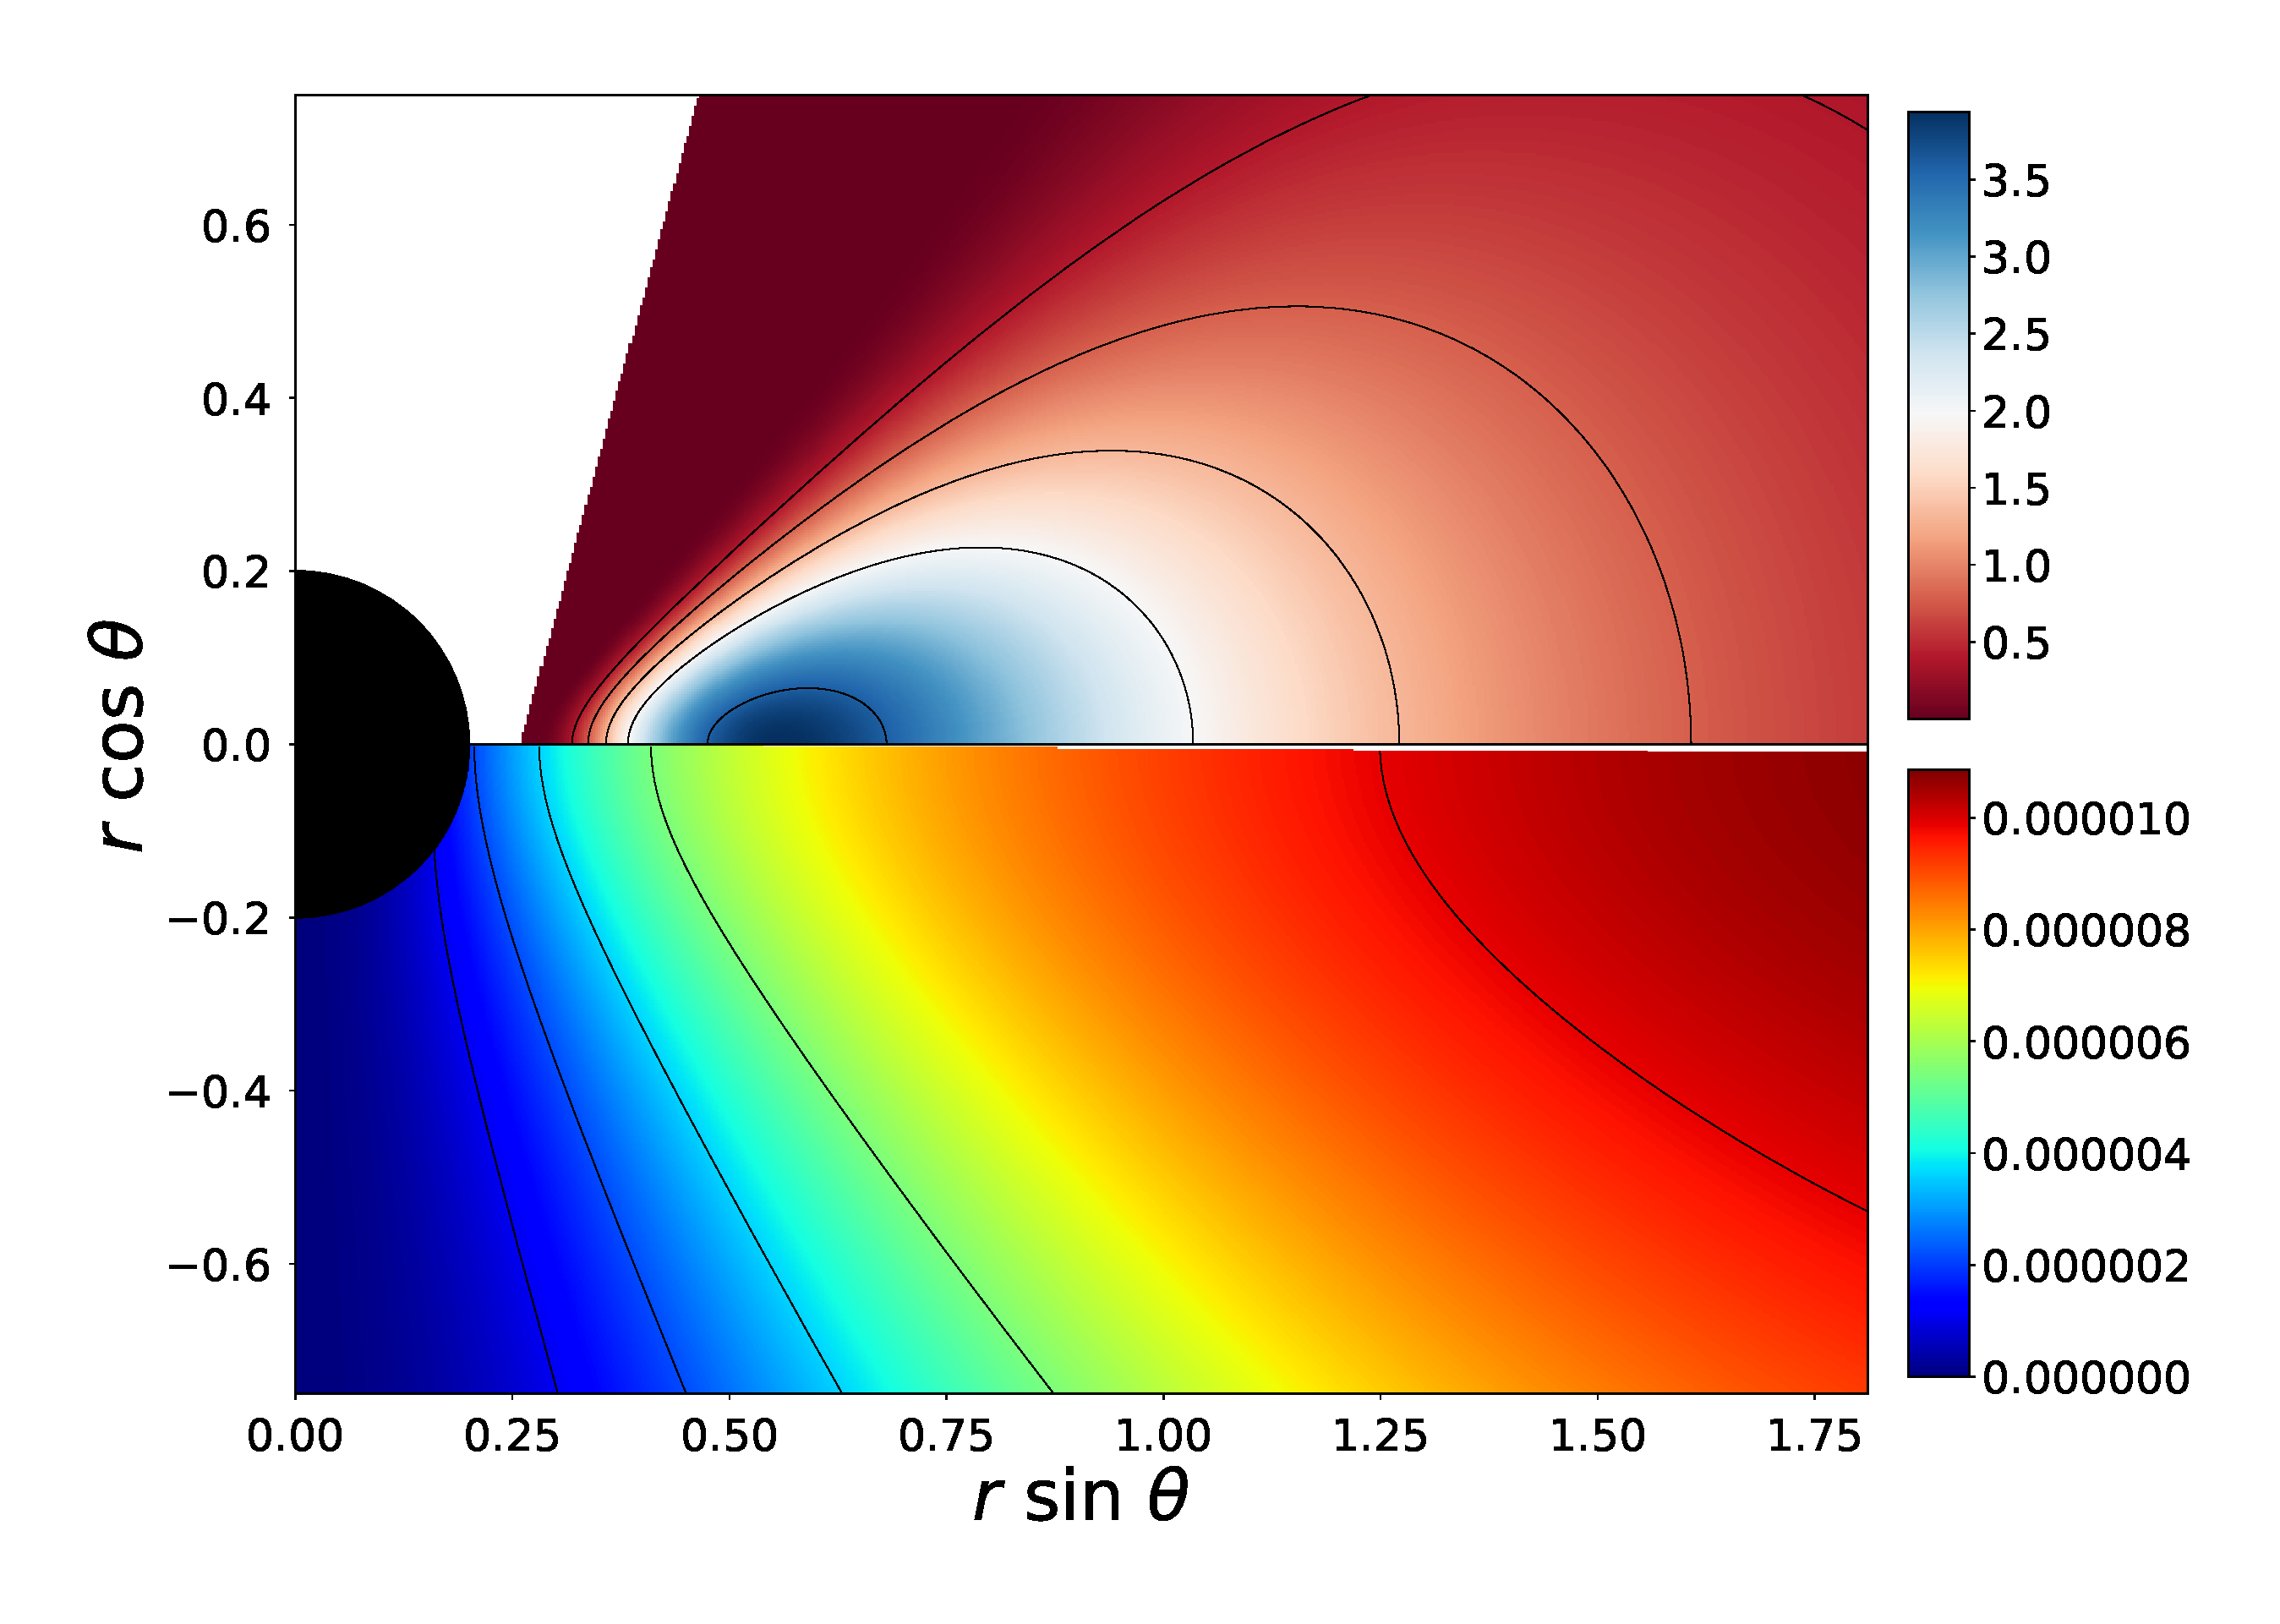
\includegraphics[scale=0.12]{figures/fig5_I_10.pdf}
\hspace{-0.3cm}
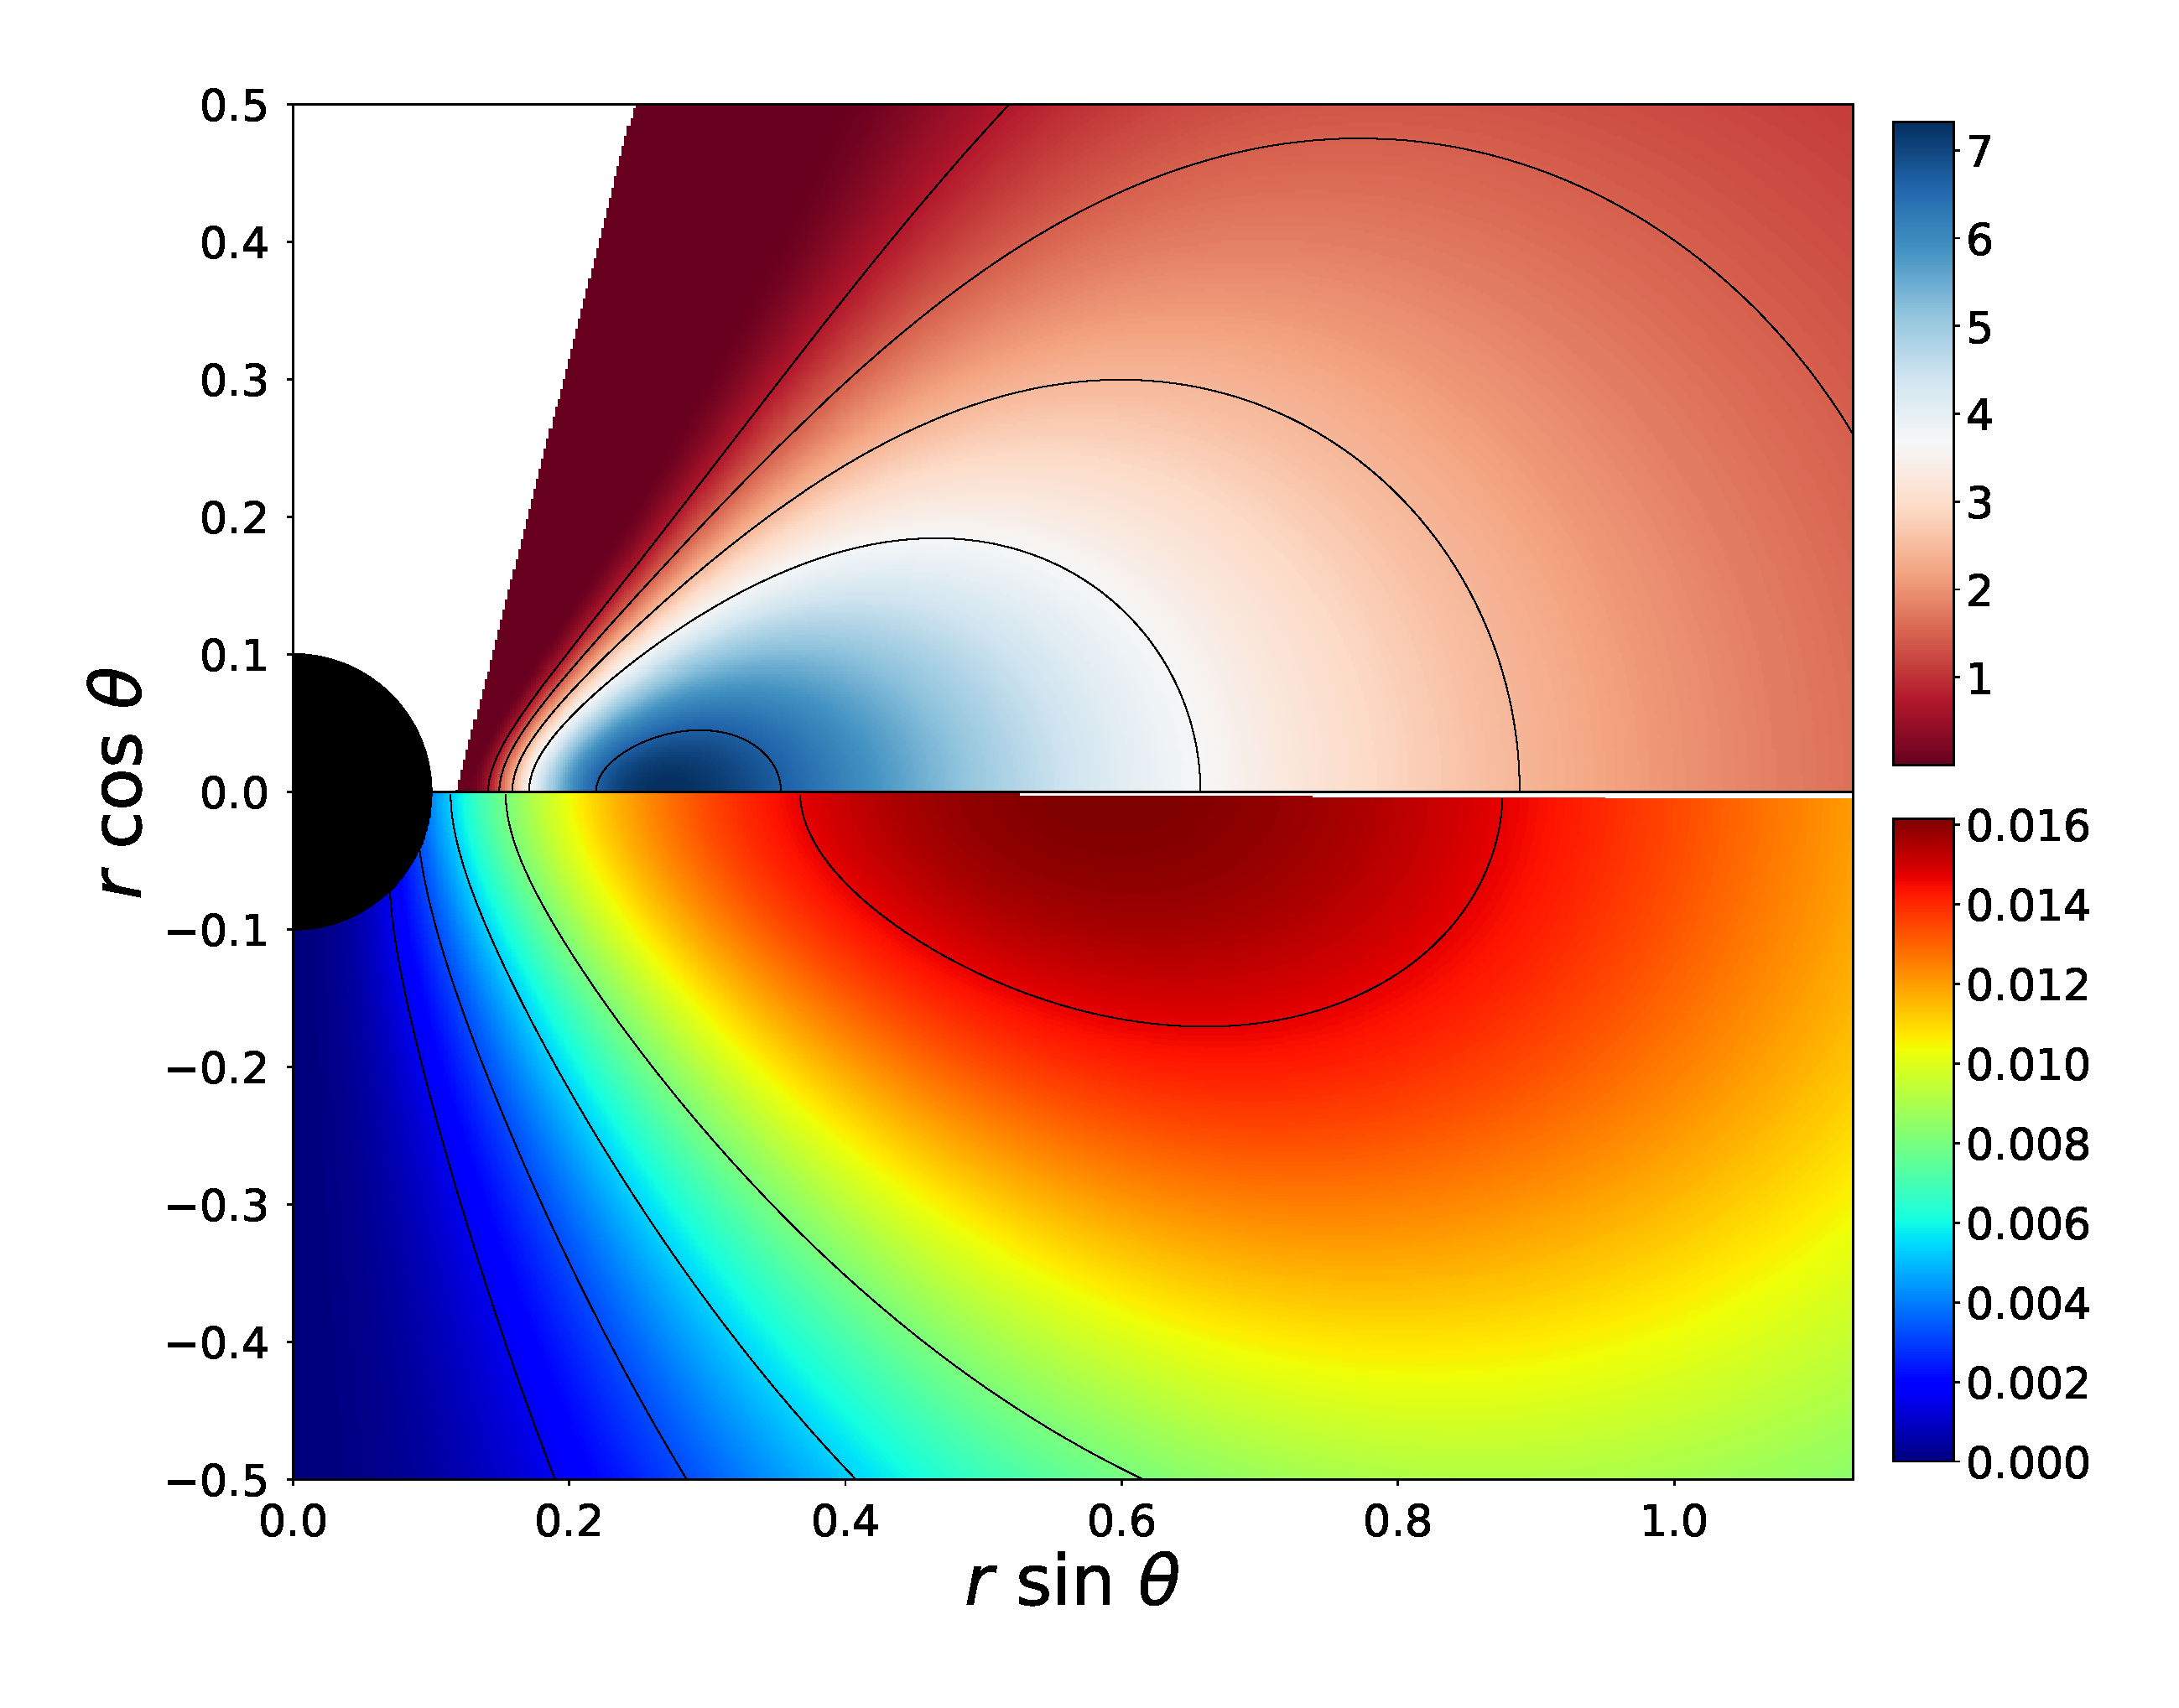
\includegraphics[scale=0.12]{figures/fig5_IV_10.pdf}
\hspace{-0.3cm}
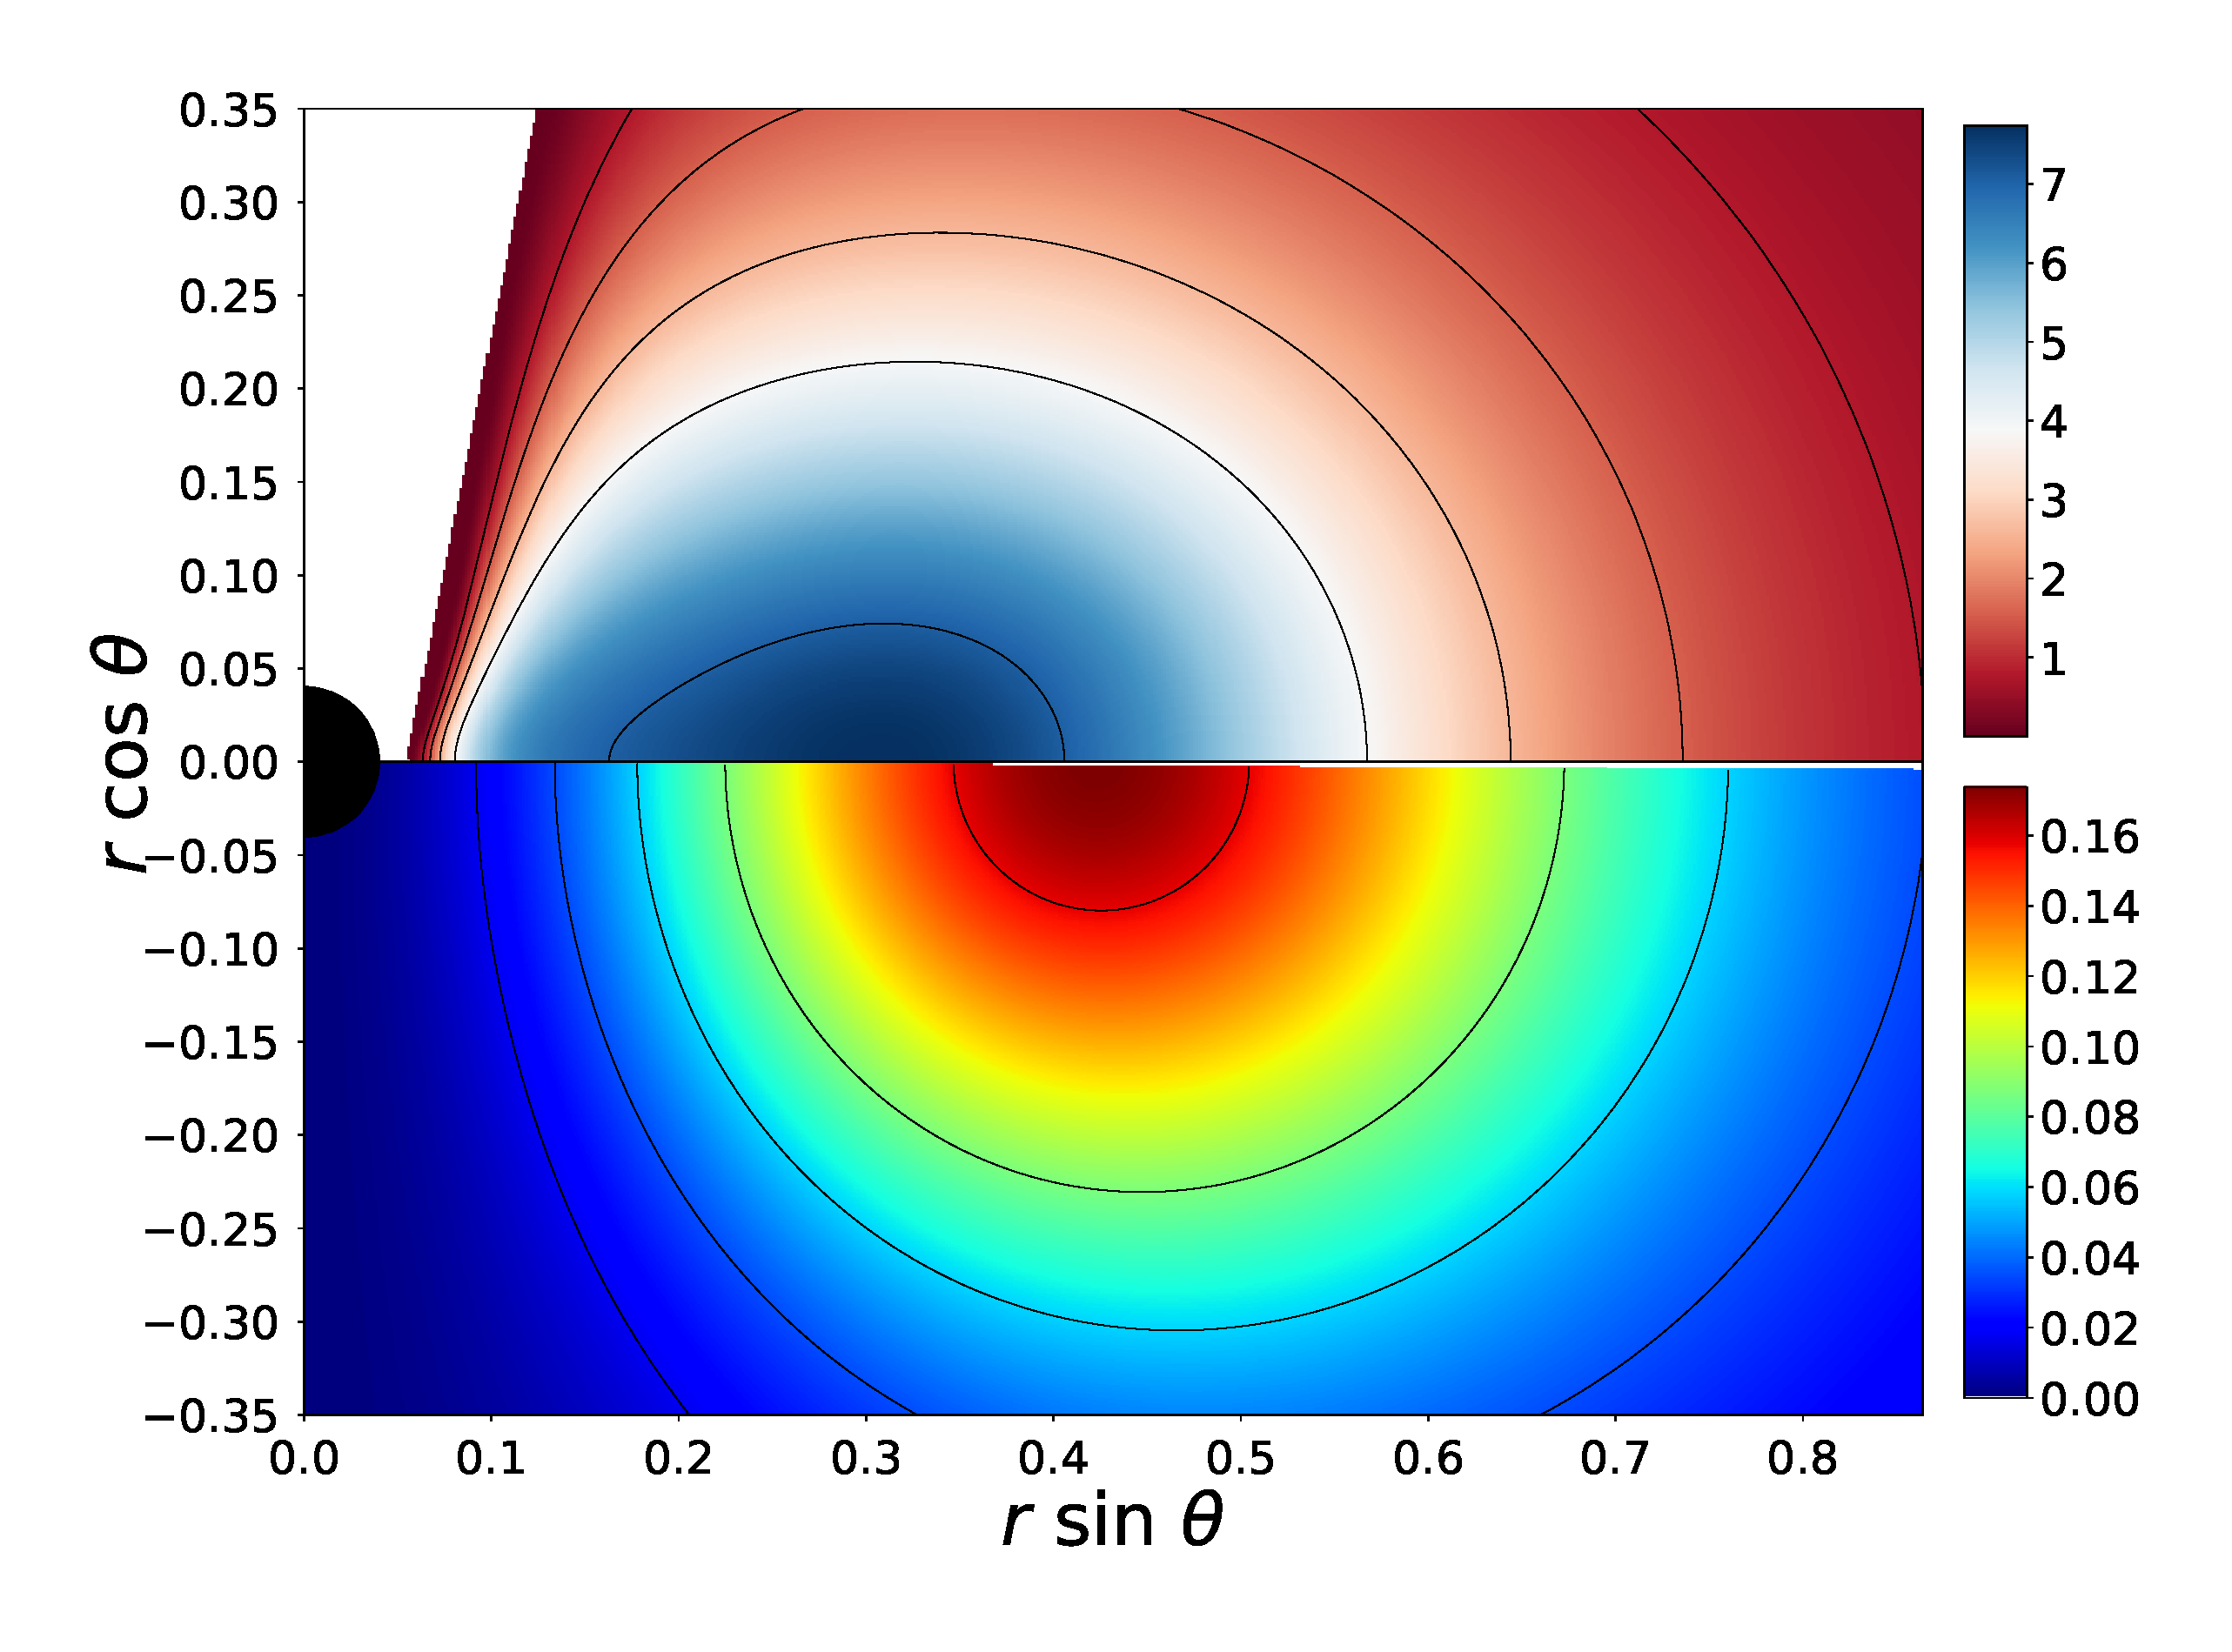
\includegraphics[scale=0.12]{figures/fig5_VII_10.pdf}
\hspace{-0.2cm}
\\
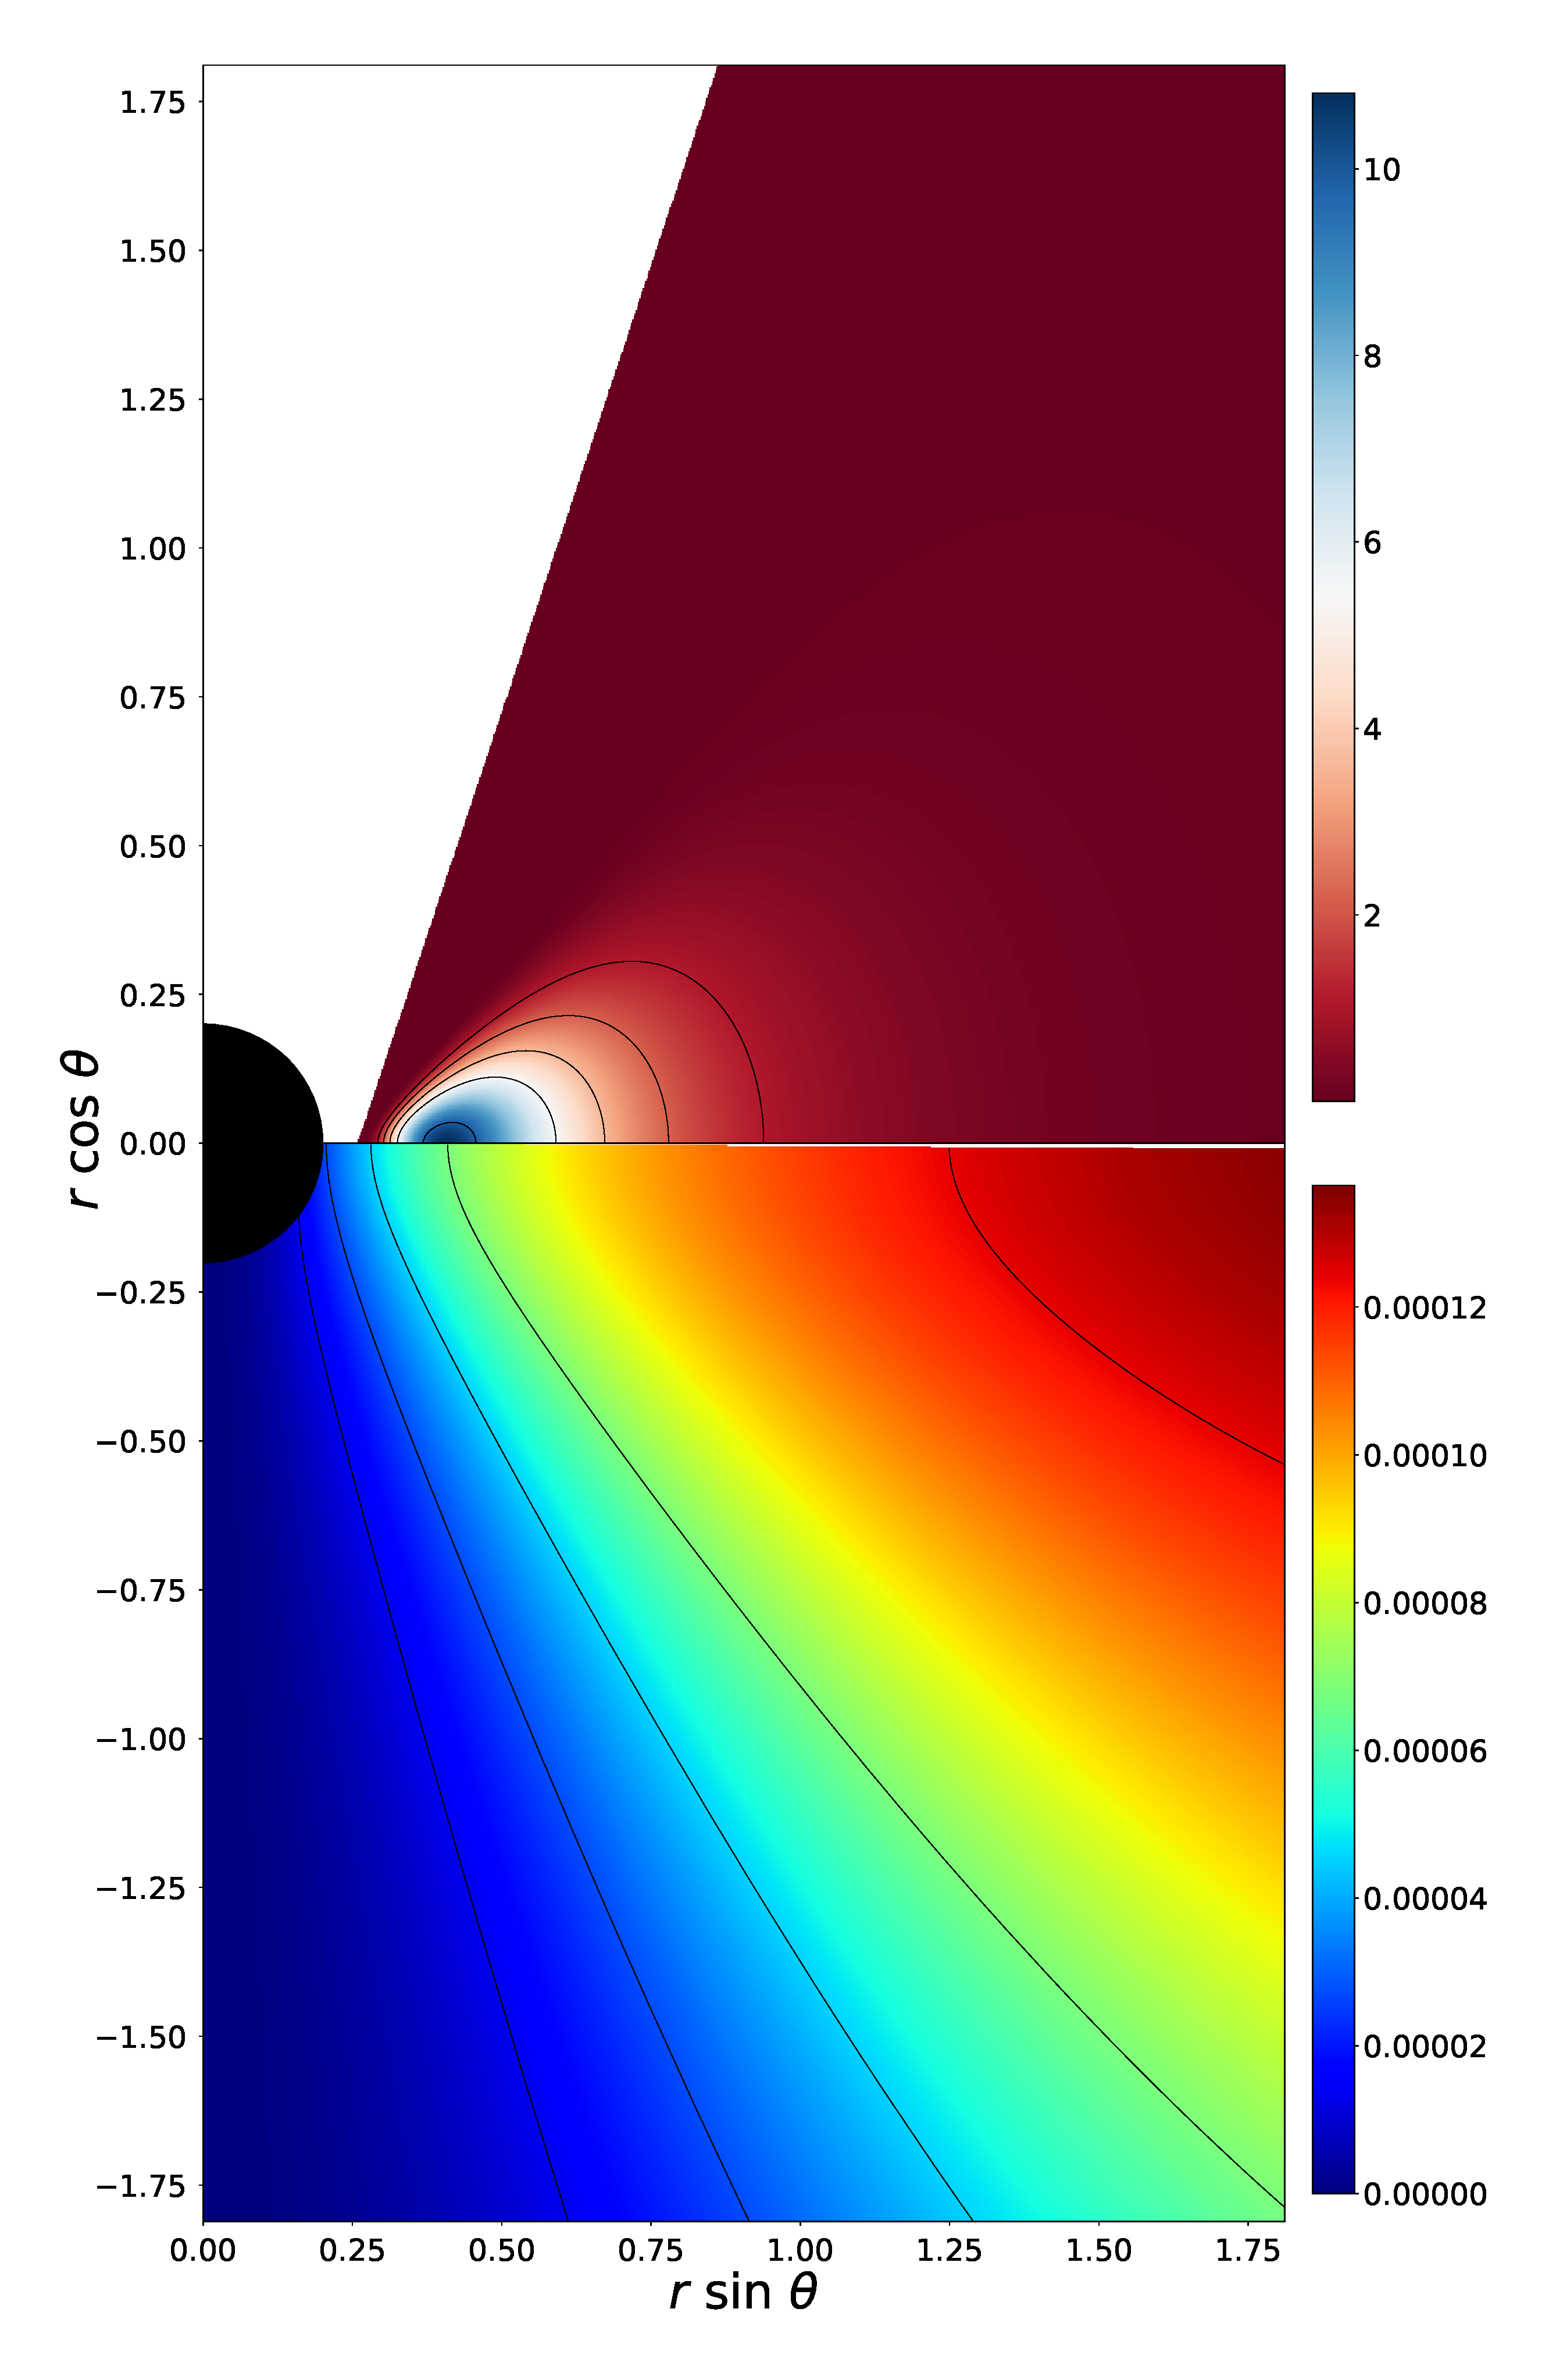
\includegraphics[scale=0.12]{figures/fig5_I__10.pdf}
\hspace{-0.3cm}
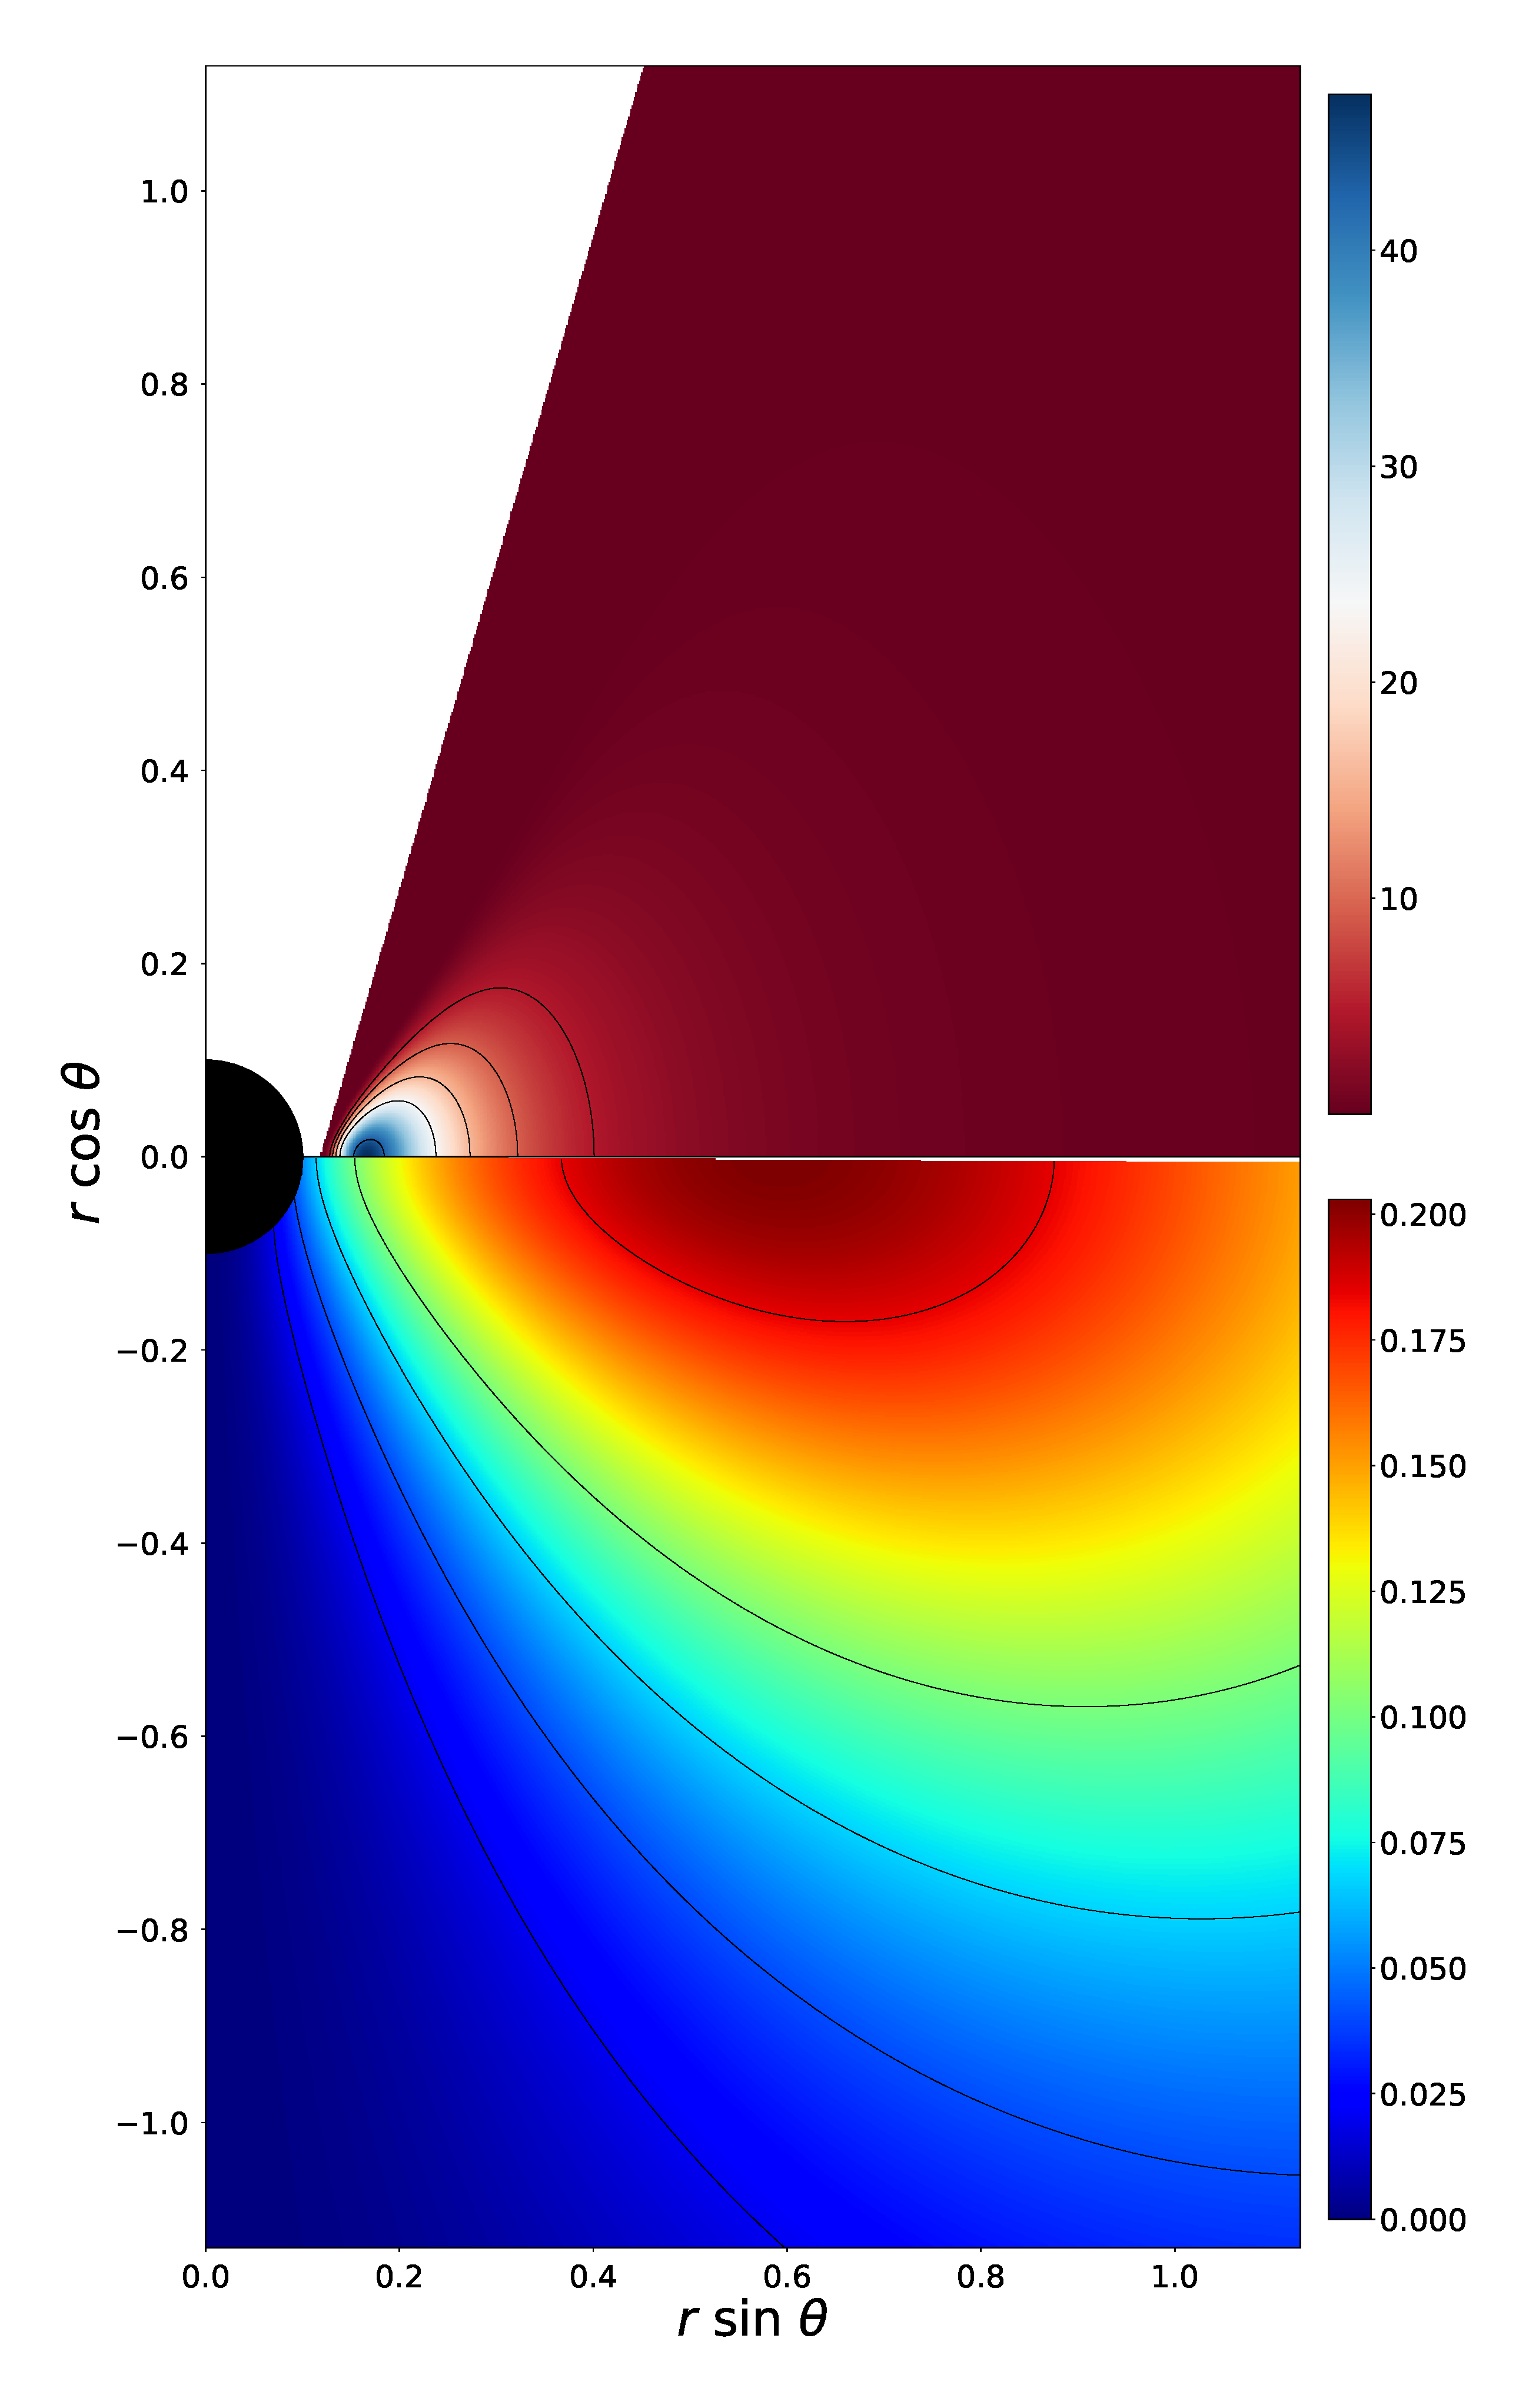
\includegraphics[scale=0.12]{figures/fig5_IV__10.pdf}
\hspace{-0.3cm}
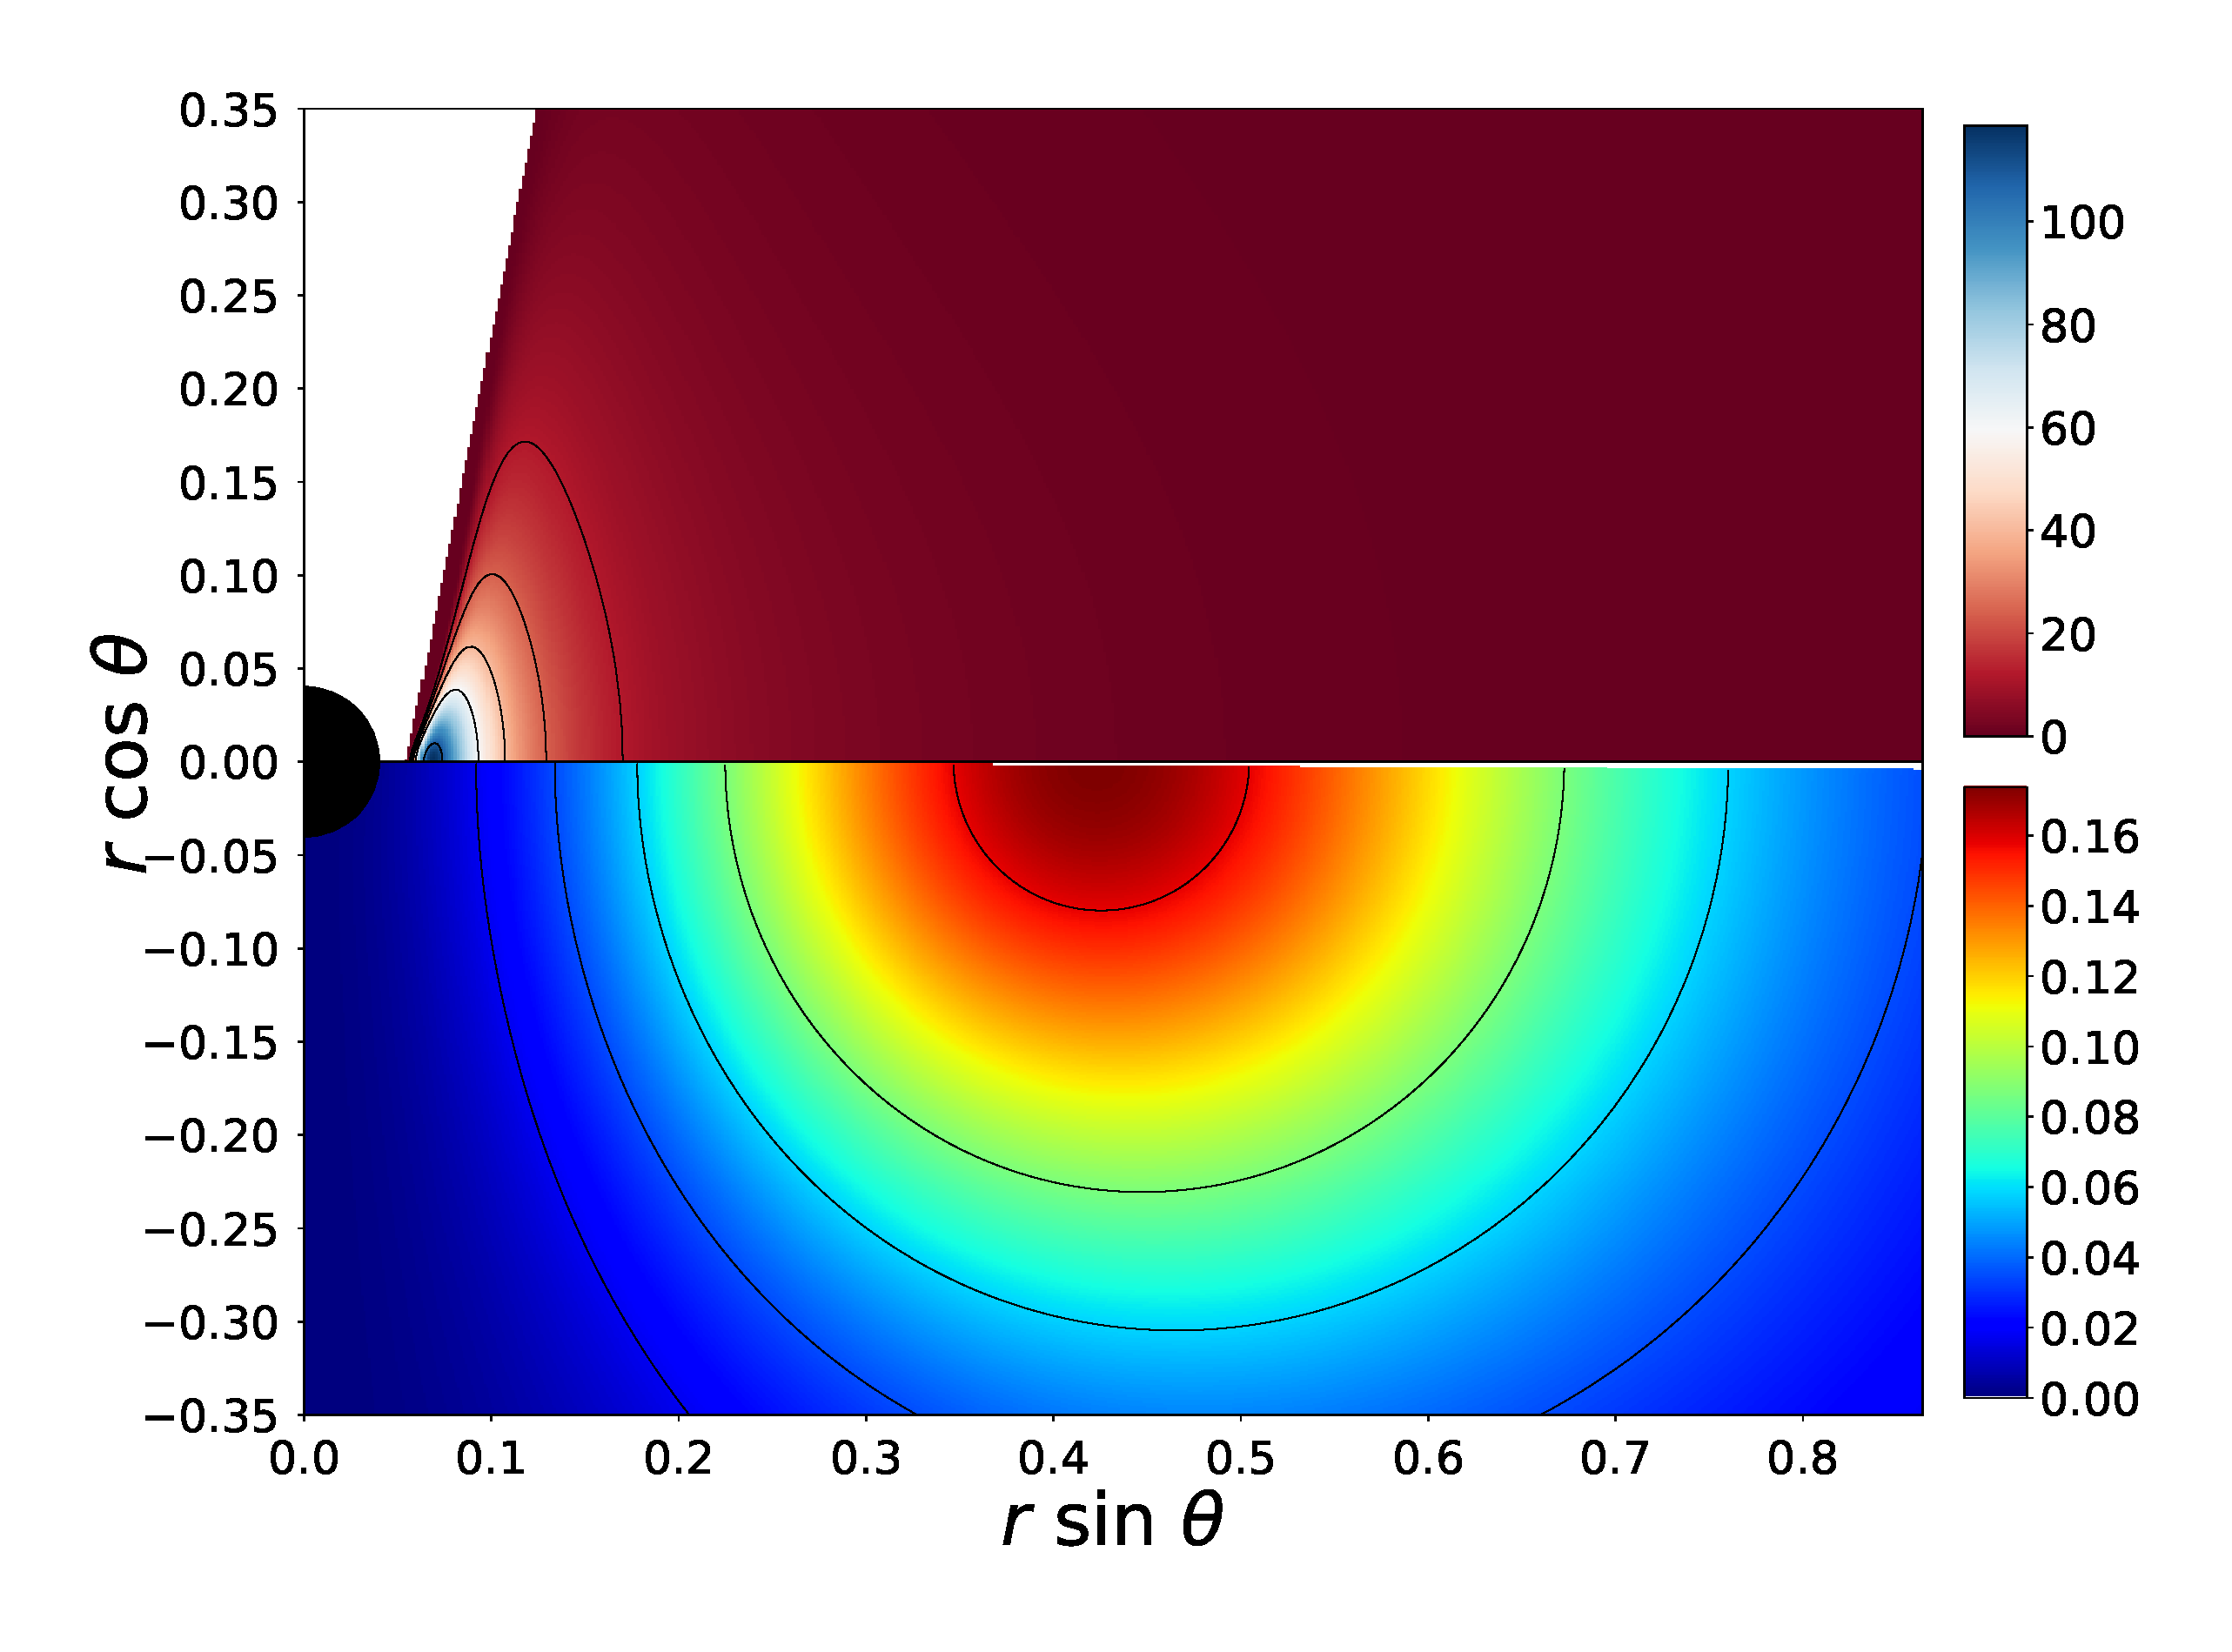
\includegraphics[scale=0.12]{figures/fig5_VII__10.pdf}
\hspace{-0.2cm}
\caption{Energy density distribution for the torus $\rho_{\mathrm{T}}$ (upper half of the images) and for the scalar field $\rho_{\mathrm{SF}}$ (lower half). From left to right the columns correspond to models I, IV, and VII. The top row corresponds to non-magnetized models ($\beta_{\mathrm{m}_{\mathrm{c}}} = 10^{10}$) and the bottom row to strongly magnetized models ($\beta_{\mathrm{m}_{\mathrm{c}}} = 10^{-10}$).
\tf{I think there is a lot of vertical space that we do not really need in these plots. To save some space, as we have many figures, I suggest to plot the vertical axis in shorter ranges, say $[-0.75,0.75]$ for model I, $[-0.5,0.5]$ for model IV, and $[-0.35,0.35]$ for model VII (and keeping the horizontal axis as it is now). I know the plot will not look squared, but that's fine.}
}
\label{comparison_mass_density}
\end{figure*}



\begin{figure*}
\centering
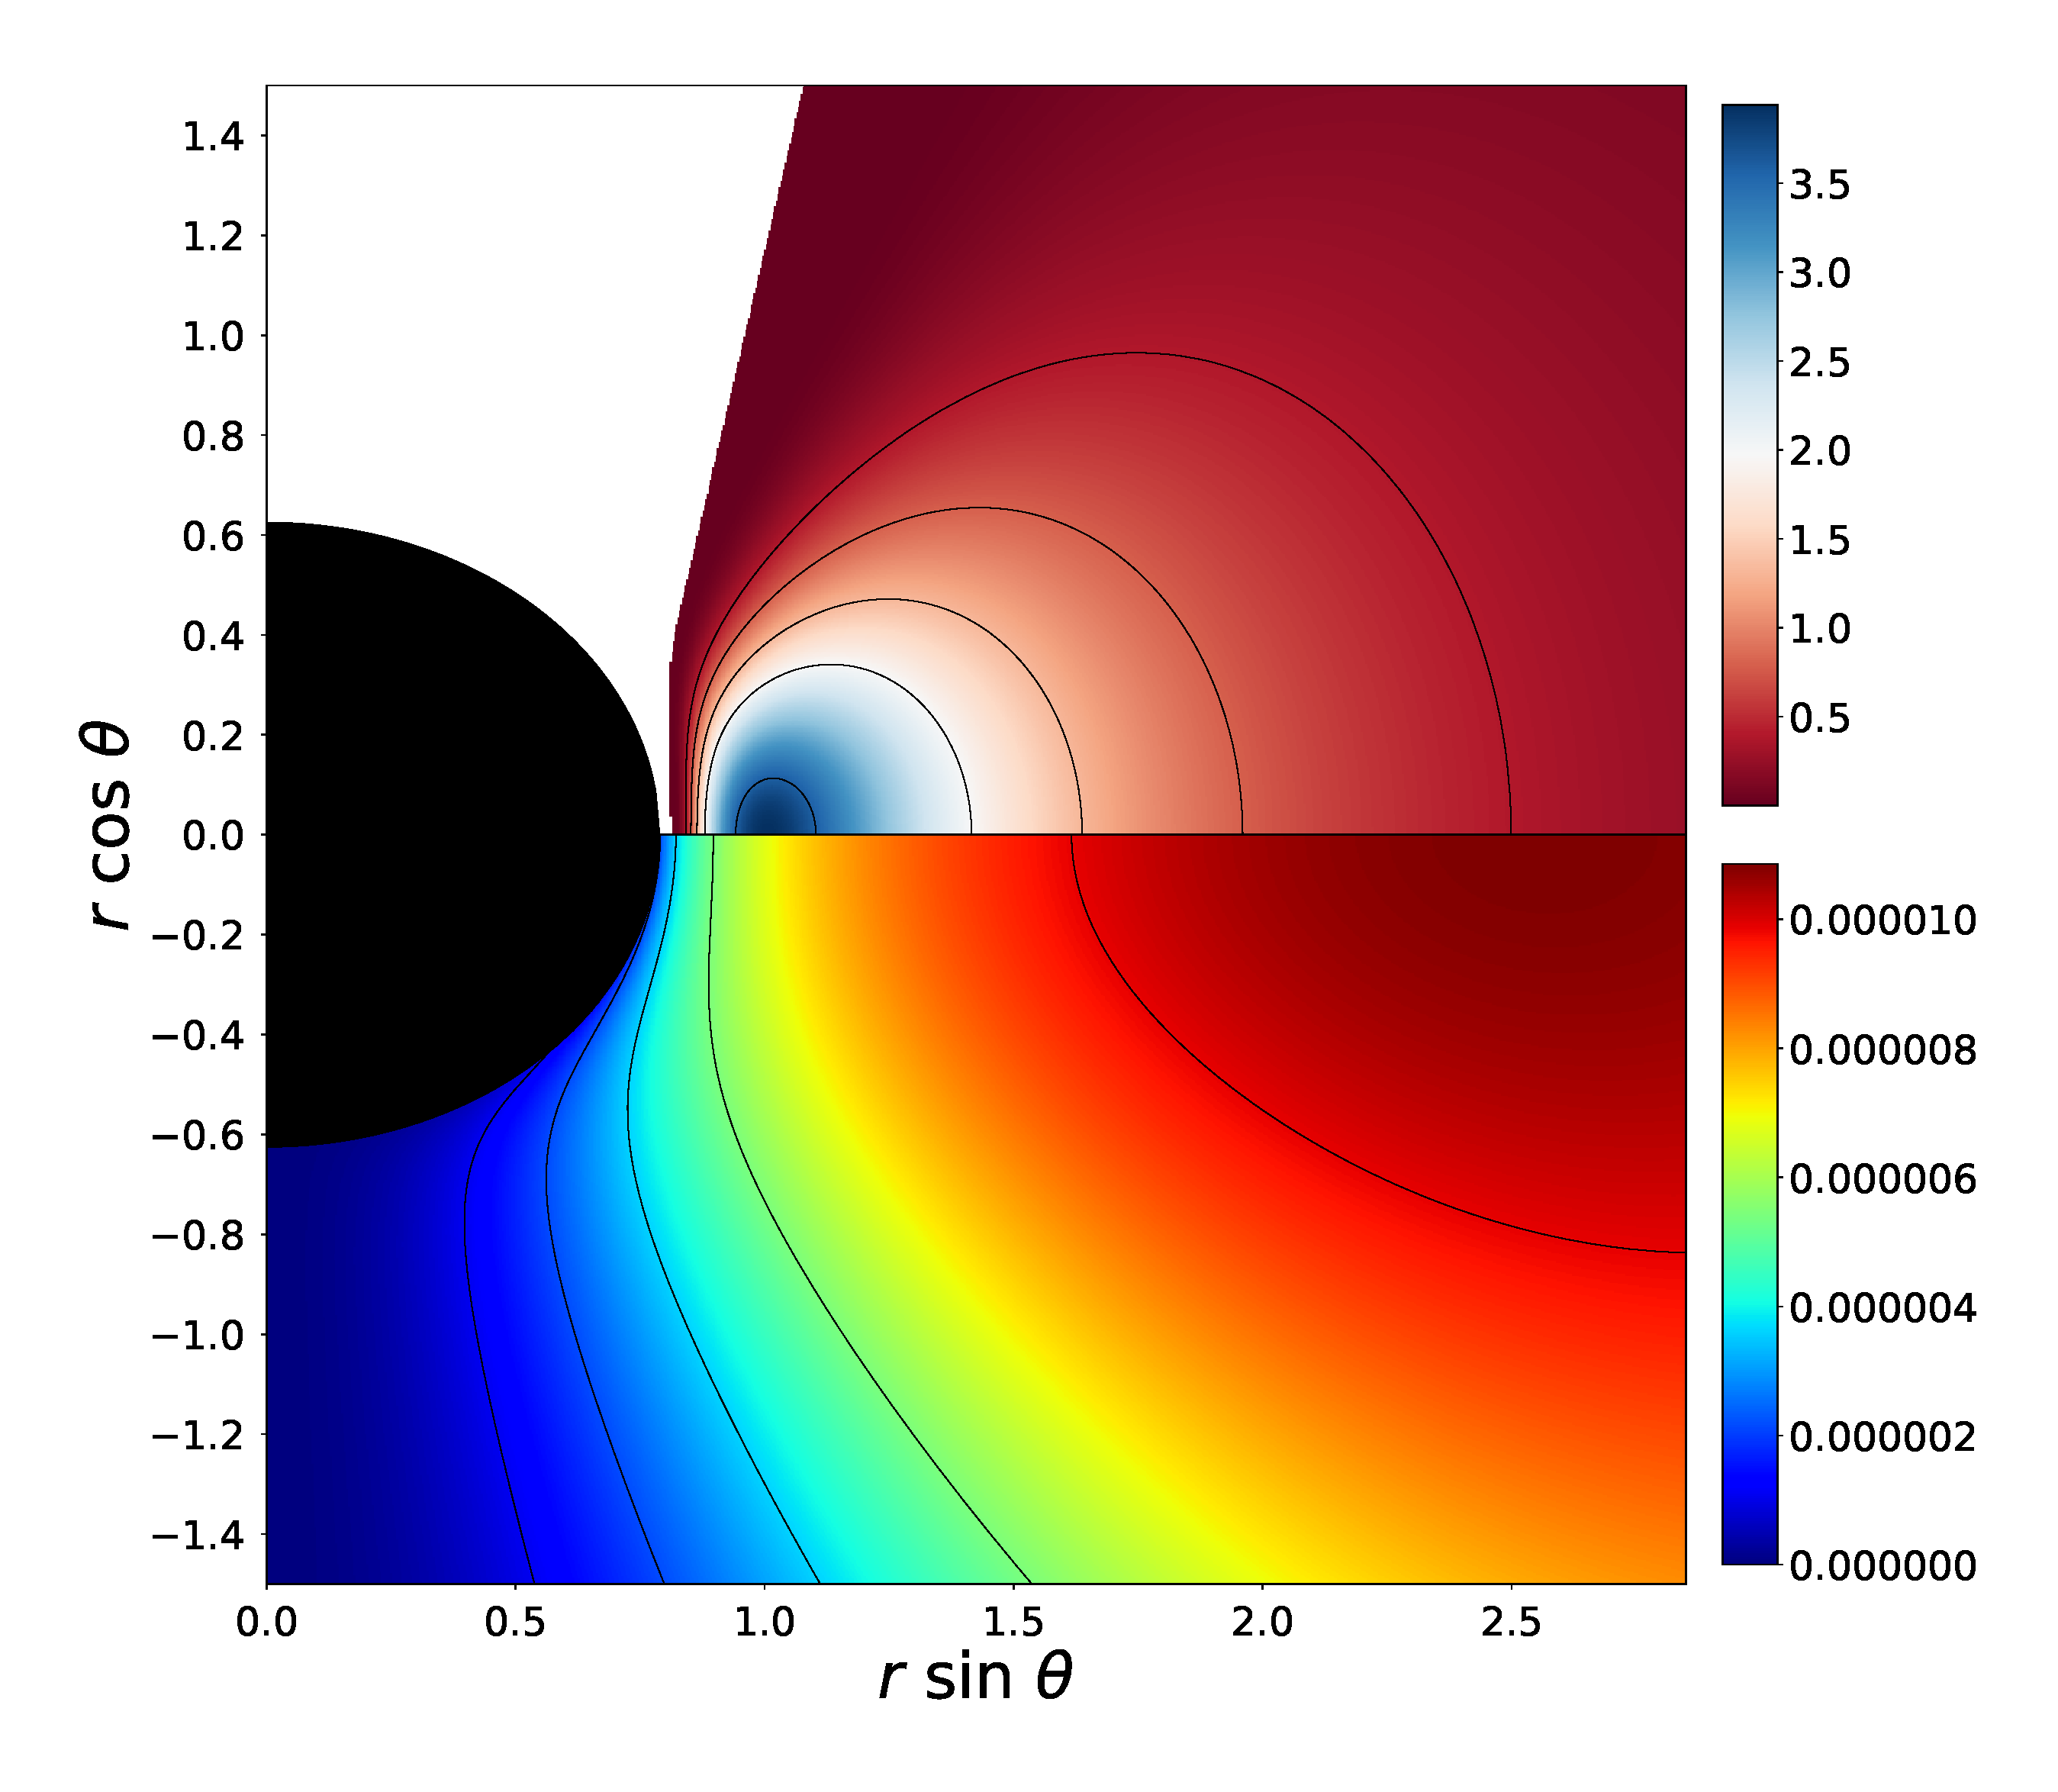
\includegraphics[scale=0.12]{figures/fig6_I_10.pdf}
\hspace{-0.4cm}
\includegraphics[scale=0.12]{figures/fig6_IV_10.pdf}
\hspace{-0.4cm}
\includegraphics[scale=0.12]{figures/fig6_VII_10.pdf}
\hspace{-0.2cm}
\\
\includegraphics[scale=0.12]{figures/fig6_I__10.pdf}
\hspace{-0.4cm}
\includegraphics[scale=0.12]{figures/fig6_IV__10.pdf}
\hspace{-0.4cm}
\includegraphics[scale=0.12]{figures/fig6_VII__10.pdf}
\hspace{-0.2cm}
\caption{Same as Fig.~\ref{comparison_mass_density} but using the perimetral radial coordinate. \tf{Same comment as in the previous figure regarding the vertical range, in this case $[-1.5,1.5]$ for all models.}}
\label{comparison_mass_density_peri}
\end{figure*}

\begin{figure*}
\centering
\includegraphics[scale=0.2]{figures/fig7_HBH_dens.eps}
\hspace{-0.cm}
\includegraphics[scale=0.2]{figures/fig7_HBH_enth.eps}
\hspace{-0.cm}
\\
\includegraphics[scale=0.2]{figures/fig7_Kerr_dens.eps}
\hspace{-0.cm}
\includegraphics[scale=0.2]{figures/fig7_Kerr_enth.eps}
\hspace{-0.cm}
\caption{Effects of the magnetization on the values for the maximum density (left) and enthalpy (right) of the disc. In the first row, we show this for all of our KBHsSH models. In the second row, we show this for a sequence of KBHs with increasing spin parameter.}
\label{comparison_HBH_Kerr_dens_enth}
\end{figure*}

\begin{figure*}
\centering
\includegraphics[scale=0.2]{figures/fig8_HBH.eps}
\hspace{0.5cm}
\includegraphics[scale=0.2]{figures/fig8_Kerr.eps}
\hspace{0.5cm}
\caption{Effects of the magnetization on the (perimeteral) location of the magnetic pressure maximum (divided by the the perimeteral radius of the centre)($R_{\mathrm{mag}, \mathrm{max}} / R_{\mathrm{c}}$). Left panel: KBHsSH models. Right panel: A sequence of KBHs with increasing spin parameter.}
\label{comparison_HBH_Kerr_r_m_max}
\end{figure*}

\begin{figure*}
\centering
\includegraphics[scale=0.14]{figures/fig9_0_10.pdf}
\hspace{-0.3cm}
\includegraphics[scale=0.14]{figures/fig9_0_1.pdf}
\hspace{-0.2cm}
\includegraphics[scale=0.14]{figures/fig9_0__10.pdf}
\\
\includegraphics[scale=0.14]{figures/fig9_05_10.pdf}
\hspace{-0.3cm}
\includegraphics[scale=0.14]{figures/fig9_05_1.pdf}
\hspace{-0.2cm}
\includegraphics[scale=0.14]{figures/fig9_05__10.pdf}
\\
\includegraphics[scale=0.14]{figures/fig9_09_10.pdf}
\hspace{-0.3cm}
\includegraphics[scale=0.14]{figures/fig9_09_1.pdf}
\hspace{-0.2cm}
\includegraphics[scale=0.14]{figures/fig9_09__10.pdf}
\\
\includegraphics[scale=0.14]{figures/fig9_09999_10.pdf}
\hspace{-0.3cm}
\includegraphics[scale=0.14]{figures/fig9_09999_1.pdf}
\hspace{-0.2cm}
\includegraphics[scale=0.14]{figures/fig9_09999__10.pdf}
\hspace{-0.2cm}
\caption{Rest-mass density distribution. From top to bottom the rows correspond to a sequence of KBHs with increasing spin parameter $a$ (0, 0.5, 0.9 and 0.9999). From left to right the columns correspond to different values of the magnetization parameter, namely non-magnetized ($\beta_{\mathrm{m}_{\mathrm{c}}} = 10^{10}$), mildly magnetized ($\beta_{\mathrm{m}_{\mathrm{c}}} = 1$) and strongly magnetized ($\beta_{\mathrm{m}_{\mathrm{c}}} = 10^{-10}$)}
\label{models_Kerr}
\end{figure*}

\begin{figure*}
\centering
\includegraphics[scale=0.14]{figures/fig10_0_10.pdf}
\hspace{-0.3cm}
\includegraphics[scale=0.14]{figures/fig10_0_1.pdf}
\hspace{-0.2cm}
\includegraphics[scale=0.14]{figures/fig10_0__10.pdf}
\\
\includegraphics[scale=0.14]{figures/fig10_05_10.pdf}
\hspace{-0.3cm}
\includegraphics[scale=0.14]{figures/fig10_05_1.pdf}
\hspace{-0.2cm}
\includegraphics[scale=0.14]{figures/fig10_05__10.pdf}
\\
\includegraphics[scale=0.14]{figures/fig10_09_10.pdf}
\hspace{-0.3cm}
\includegraphics[scale=0.14]{figures/fig10_09_1.pdf}
\hspace{-0.2cm}
\includegraphics[scale=0.14]{figures/fig10_09__10.pdf}
\\
\includegraphics[scale=0.14]{figures/fig10_09999_10.pdf}
\hspace{-0.3cm}
\includegraphics[scale=0.14]{figures/fig10_09999_1.pdf}
\hspace{-0.2cm}
\includegraphics[scale=0.14]{figures/fig10_09999__10.pdf}
\hspace{-0.2cm}
\caption{Rest-mass density distribution using perimeteral coordinates. From top to bottom the rows correspond to a sequence of KBHs with increasing spin parameter $a$ (0, 0.5, 0.9 and 0.9999). From left to right the columns correspond to different values of the magnetization parameter, namely non-magnetized ($\beta_{\mathrm{m}_{\mathrm{c}}} = 10^{10}$), mildly magnetized ($\beta_{\mathrm{m}_{\mathrm{c}}} = 1$) and strongly magnetized ($\beta_{\mathrm{m}_{\mathrm{c}}} = 10^{-10}$)}
\label{models_Kerr_peri}
\end{figure*}


\begin{table*}[t]
\caption{Disc parameters and values of their relevant physical magnitudes for the KBH case. For all the cases, we have $R_{\mathrm{in}} = R_{\mathrm{mb}}$ , $l = l_{\mathrm{mb}}$ and $M_{\mathrm{BH}} = 1$.}        
\label{KBH_disk_parameters}      
\centering          
\begin{tabular}{c c c c c  c c c c c c c}
\hline\hline       
 $a$ & $l$ & $W_{\mathrm{c}}$ & $R_{\mathrm{in}}$ & $R_{\mathrm{c}}$ &  $\beta_{\mathrm{m_{\mathrm{c}}}}$ & $h_{\mathrm{max}}$ & $\rho_{\mathrm{max}}$ & $p_{\mathrm{max}}$ & $p_{\mathrm{m, max}}$ & $R_{\mathrm{max}}$ & $R_{\mathrm{m, max}}$\\ 
\hline           
$0$ & $4.00$ & $-4.32 \times 10^{-2}$ & $4.00$ & $10.47$ & $10^{10}$ & $1.04$ & $1.0$ & $1.10 \times 10^{-2}$ & $1.15 \times 10^{-12}$ & $10.47$ & $11.86$\\ 
 \hline 
 &  &  &  &  & $1$ & $1.02$ & $1.11$ & $6.29 \times 10^{-3}$ & $5.69 \times 10^{-3}$ & $8.81$ & $9.52$\\ 
 \hline 
 &  &  &  &  & $10^{-10}$ & $1.0$ & $1.48$ & $1.83 \times 10^{-12}$ & $1.48 \times 10^{-2}$ & $7.70$ & $8.14$\\ 
 \hline 
 $0.5$ & $3.41$ & $-6.35 \times 10^{-2}$ & $2.99$ & $7.12$ & $10^{10}$ & $1.07$ & $1.0$ & $1.64 \times 10^{-2}$ & $1.72 \times 10^{-12}$ & $7.19$ & $8.14$\\ 
 \hline 
 &  &  &  &  & $1$ & $1.03$ & $1.12$ & $9.43 \times 10^{-3}$ & $8.47 \times 10^{-3}$ & $6.05$ & $6.53$ \\ 
 \hline 
 &  &  &  &  & $10^{-10}$ & $1.0$ & $1.53$ & $2.81 \times 10^{-12}$ & $2.23 \times 10^{-2}$ & $5.29$ & $5.59$\\ 
\hline  
$0.9$ & $2.63$ & $-0.129$ & $2.18$ & $3.78$ & $10^{10}$ & $1.14$ & $1.0$ & $1.64 \times 10^{-2}$ & $3.65 \times 10^{-12}$ & $3.78$ & $4.23$\\ 
 \hline 
 &  &  &  &  & $1$ & $1.07$ & $1.14$ & $2.03 \times 10^{-2}$ & $1.78 \times 10^{-2}$ & $3.25$ & $3.47$\\ 
 \hline 
 &  &  &  &  & $10^{-10}$ & $1.0$ & $1.70$ & $6.54 \times 10^{-12}$ & $4.92 \times 10^{-2}$ & $2.92$ & $3.04$ \\ 
 \hline 
$0.9999$ & $2.02$ & $-0.429$ & $2.00015$ & $2.034$ & $10^{10}$ & $1.54$ & $1.0$ & $0.134$ & $1.61 \times 10^{-11}$ & $2.034$ & $2.094$ \\ 
\hline 
 &  &  &  &  & $1$ & $1.29$ & $1.51$ & $0.110$ & $7.52 \times 10^{-2}$ & $2.0075$ & $2.014$\\ 
\hline 
 &  &  &  &  & $10^{-10}$ & $1.0$ & $6.17$ & $1.22 \times 10^{-10}$ & $0.491$ & $2.0021$ & $2.0030$ \\ 
\hline   
\end{tabular}
\end{table*}


Table~\ref{KBH_disk_parameters} reports the relevant physical quantities for the disks built around KBH. \tf{Describe.}

In figure~\ref{comparison_mass_density} we show the total energy density of the torus $\rho_{\mathrm{T}}$ (upper half of each image) and the total energy density of the scalar field $\rho_{\mathrm{SF}}$ (lower half) for models I, IV and VII and 2 values of the magnetization parameter at the center ($10^{10}$, left panel, and $10^{-10}$, right panel). \tf{Describe this figure.} 

In figure~\ref{comparison_mass_density_peri}, we show the same, but using the perimeteral coordinate we defined earlier. The plots show that the maximum of the total energy density of the disk $\rho_{\mathrm{t}}$ is closer to the maximum of the total energy density of the scalar field $\rho_{\mathrm{SF}}$ for increasing hair. \tf{This trend is only satisfied for the unmagnetized models (top row) but not for the strongly magnetized models.}

\tf{One question: in our approach we are building the disks using the stress-energy tensor of the fluid only. Is this correct? Shouldn't we consider the entire stress-energy tensor from the fluid and the scalar field? Is this a valid approximation because we are in the test-fluid regime? What did~\cite{Vincent:2016} do?}

\subsection{Comparison with KBHs}

Also, in figures~\ref{models_Kerr} and~\ref{models_Kerr_peri} we show different KBH models with the same mass $M_{\mathrm{BH}} = 1$ and different values for the spin parameter($0$, $0.5$, $0.9$, $0.9999$). 

As shown in~\cite{Delgado:2018} some \sg{(compute which ones are embeddable and which are not)} of our models are in the region of the domain of existence where the event horizon is not embeddable in $\mathbb{E}^3$ then, the shaded regions depicting the horizon that we show at several of the figures are not faithful representations of the horizon geometry. Nevertheless, we show them for the sake of clarity. Also, this led us to asking ourselves if this could also happen for the shape of the accretion tori and therefore, we should be conservative when extracting information about the morphology of the disks from 2-dimensional plots. This idea is discussed in appendix~\ref{torus_embedding}.

%%%%%%%%%%%%%%%%%%
\subsection{Magnetization profiles}
%%%%%%%%%%%%%%%%%%

The dependence of the maximum specific enthalpy $h_{\mathrm{max}}$ and the maximum rest-mass density $\rho_{\mathrm{max}}$ with the magnetization parameter is shown in figures~\ref{comparison_HBH_Kerr_dens_enth}. The upper panels correspond to the KBHsSH models (I-VII) and the lower ones to a sequence of KBHs with increasing spin parameter. \tf{Maybe there is an excessive number of cases for KBHs. Maybe it's enough to only include the four cases we have in Table III. We could always indicate in the main text the values that are reached for an extreme value of $a$ with seven 9. This will also simplify the presentation of this figure, where I don't like very much having lines and dots.} Here we can see that, for both cases, an increase in $|\Delta W|$ implies higher values for $h_{\mathrm{max}}$ (low magnetization) and also higher values for $\rho_{\mathrm{max}}$ (high magnetization). However, there are differences between the two cases. For the enthalpy, the values of $h_{\mathrm{max}}$ reached for the KBHsSH are much higher than those of the KBH case. This fact tells us that, while the $w = \rho h \simeq \rho$ approximation (see \cite{Komissarov:2006} and \cite{Gimeno-Soler:2017}) is valid for magnetized flows ($\beta_{\mathrm{m_c}} \sim 1$) for reasonable values of the spin parameter ($a \sim 0.99$ or lower), that is not the case for KBHsSH. Also, for the rest-mass density we have a different behaviour: $\rho_{\mathrm{max}}$ for KBHsSH reach values only attainable by high spin parameter KBHs (between $a = 0.9$ and $a = 0.99999$ for the seven models we present here).

Figure~\ref{comparison_HBH_Kerr_r_m_max} shows the variation of the quotient of the perimeteral radius of the magnetic pressure maximum by the perimeteral radius of the disk center $R_{\mathrm{m, max}}/R_{\mathrm{c}}$ with the decimal logarithm of the magnetization parameter at the disk center $\log_{10} \beta_{\mathrm{m_c}}$ for the same KBHsSH and KBH cases as in figure~\ref{comparison_HBH_Kerr_dens_enth}. The inset shows a region around $\beta_{\mathrm{m_c}} = 3$ and $R_{\mathrm{m, max}}/R_{\mathrm{c}} = 1$, this is because for disks with $h = 1$, $R_{\mathrm{m, max}} = R_{\mathrm{c}}$ if $\beta_{\mathrm{m_c}} = 1 / \Gamma - 1$. As we can easily see, this condition is also fulfilled for the Kerr case, even $h \neq 1$ (with a slight deviation for very high spin parameter cases), but not quite for the KBHsSH cases.



\sg{Include discussion about radial profiles.}





%\begin{table}
%\caption{List of models of KBHsSH.}        
%\label{models_list}      
%\centering          
%\begin{tabular}{c c c c  c c c c}
%\hline\hline       
% Model & $M_{\mathrm{ADM}}$ & $J_{\mathrm{ADM}}$ & $M_{\mathrm{H}}$ &  $J_{\mathrm{H}}$ & $M_{\mathrm{SF}}$ & $J_{\mathrm{SF}}$ & $r_{\mathrm{H}}$ \\ 
%\hline           
%I & $0.415$ & $0.172$ & $0.393$ &  $0.15$  & $0.022$ & $0.022$ & $0.2$\\ 
% \hline 
%II & $0.630$ & $0.403$ & $0.340$ &  $0.121$  & $0.063$ & $0.282$ & $0.221$ \\
% \hline 
%III & $0.797$ & $0.573$ & $0.365$ &  $0.172$  & $0.573$ & $0.432$ & $0.111$ \\ 
% \hline 
%IV & $0.933$ & $0.739$ & $0.234$ &  $0.114$  & $0.699$ & $0.625$ & $0.1$ \\ 
% \hline 
%V & $0.940$ & $0.757$ & $0.159$ &  $0.076$  & $0.757$ & $0.781$ & $0.091$ \\ 
% \hline 
%VI & $0.959$ & $0.795$ & $0.087$ &  $0.034$  & $0.872$ & $0.781$ & $0.088$ \\ 
% \hline 
%VII & $0.975$ & $0.85$ & $0.018$ &  $0.002$  & $0.957$ & $0.848$ & $0.04$ \\ 
%\hline      
%\end{tabular}
%\end{table}
%
%\begin{table}
%\caption{Values of the normalized spin parameter for the ADM quantities ($a_{\mathrm{ADM}}$), for the BH horizon quantities ($a_{\mathrm{H}}$), the horizon linear velocity ($v_{\mathrm{H}}$) and the spin parameter corresponding to a KBH with a linear velocity equal to $v_{\mathrm{H}}$, ($a_{\mathrm{H_{eq}}}$).}        
%\label{models_spin_vel}      
%\centering          
%\begin{tabular}{c c c c c}
%\hline\hline       
% Model & $a_{\mathrm{ADM}}$ & $a_{\mathrm{H}}$ & $v_{\mathrm{H}}$ & $a_{\mathrm{H_{eq}}}$ \\ 
%\hline           
%I & $0.9987$ & $0.9712$ & $0.7685$ & $0.9663$ \\ 
% \hline 
%II & $1.014$ & $0.3760$ & $0.6802$ & $0.9301$ \\
% \hline 
%III & $0.9032$ & $1.295$ & $0.7524$ & $0.9608$ \\ 
% \hline 
%IV & $0.8489$ & $2.082$ & $0.5635$ & $0.8554$ \\ 
% \hline 
%V & $0.8560$ & $3.017$ & $0.4438$ & $0.7415$ \\ 
% \hline 
%VI & $0.9477$ & $3.947$ & $0.2988$ & $0.5487$ \\ 
% \hline 
%VII & $0.8941$ & $6.173$ & $0.09732$ & $0.1928$ \\ 
%\hline      
%\end{tabular}
%\end{table}


%%%%%%%%%%%%
\section{Conclusions}
\label{conclusions}
%%%%%%%%%%%%

Future work: Non-constant angular momentum case, Proca hair, shadows of the system HBH+disk.

\begin{acknowledgements}

\end{acknowledgements}

\bibliographystyle{apsrev4-1}
\bibliography{references.bib}

\begin{appendix}
% \section{Embedding of the accretion torus in $\mathbb{E}^3$}\label{torus_embedding}
% Following the same reasoning as in~\cite{Delgado:2018}, we write the 2-metric for the surface of a torus as 
% \begin{equation}\label{eq:torus_prev_metric}
% \mathrm{d}\sigma^2 = \frac{e^{2 F_1}}{N}\mathrm{d}r^2+ e^{2 F_1}r^2\mathrm{d}\theta^2+e^{2 F_2} r^2 \sin^2\theta \mathrm{d}\phi^2,
% \end{equation}
% and the condition $r = r(\theta)$ for the surface of the torus. The location of the surface of the torus $r(\theta)$ can be obtained integrating $r' = \frac{\mathrm{d}r}{\mathrm{d}\theta} = -\frac{\partial_{\theta}W}{\partial_{r}W}$ (equation (24) of~\citep{Gimeno-Soler:2017}). Using this, we can write equation~\eqref{eq:torus_prev_metric} as
% \begin{equation}\label{eq:torus_metric}
% \mathrm{d}\sigma^2 = e^{2 F_1} \mathrm{d}\theta^2\left(\frac{r'^2}{N} +r^2\right)+e^{2 F_2} r^2 \sin^2\theta \mathrm{d}\phi^2,
% \end{equation}
% with the prime $'$ denoting partial differentiation with respect to $\theta$. Then, we try the embedding in $\mathbb{E}^3$ with the Cartesian metric $\mathrm{d}\sigma^2 = \mathrm{d}X^2 + \mathrm{d}Y^2 + \mathrm{d}Z^2$ and the embedding functions:
% \begin{equation}
% X + \mathrm{i}Y = f(\theta)e^{\mathrm{i}\phi},  \;\;\; Z = g(\theta),
% \end{equation}
% then
% \begin{equation}
% f = e^{2 F_2} r^2 \sin^2\theta, \;\;\; f'^2 + g'^2 = e^{2 F_1}\left(\frac{r'^2}{N} +r^2\right),
% \end{equation}
% so we can write $g'^2$ as
% \begin{equation}\label{eq:embedding_existance}
% g'^2 = e^{2 F_1}\left(\frac{r'^2}{N} +r^2\right) - e^{2 F_2} (F_2'r \sin \theta + r' \sin \theta + r \cos \theta)^2.
% \end{equation}
% This result tells us that the r.h.s. of~\eqref{eq:embedding_existance} must be $\geq 0$ in order to the embedding function to exist.

% \begin{figure*}
% \centering
% \includegraphics[scale=0.2]{figures/embedding.pdf}
% \hspace{0.5cm}
% \caption{Rest-mass density distribution for model VII with $r_{\mathrm{in}} = 0.08$ and $\beta_{\mathrm{m_c}} = 10^{10}$ (up) and the scalar field amplitude distribution $\phi$ (down). The isocontours are blue when the r.h.s. of equation~\eqref{eq:embedding_existance} is $> 0$ and red when is $\leq 0$.}
% \label{embedding_VII}
% \end{figure*}

\section{Finding $l_{\mathrm{mb}}$ and $r_{\mathrm{mb}}$}\label{ang_mom_appendix}
\sg{I figured this out, but now I am not really sure if this is interesting enough to be an appendix by itself. Maybe more like a comment in the main text.}
\end{appendix}     

\end{document}


